\documentclass[12pt]{article}
\pdfminorversion=6

%, , , , , , , , , , , , , , , , , , , , , , , -
% Neural Computation (MIT Press) submission format -- review draft.
%   * article class, 12pt, single column, double-spaced
%   * 1-inch margins, Times Roman text + math
%   * author-year citations (NC house style)
% For the final accepted version, MIT Press uses their own production
% template; see https://direct.mit.edu/neco for current guidelines.
%, , , , , , , , , , , , , , , , , , , , , , , -

\usepackage[round,authoryear,sort&compress]{natbib}
\usepackage[margin=1in]{geometry}
\usepackage{mathptmx}            % Times Roman text + math
\usepackage{setspace}
\onehalfspacing
\usepackage{placeins}
\usepackage{float}
\usepackage{sidecap}
\sidecaptionvpos{figure}{c}
\usepackage{amsmath, amssymb, mathtools, amsthm}
\usepackage{bm}
\usepackage{enumitem}
\usepackage{graphicx}
\graphicspath{{../}{./}}
\usepackage{booktabs}
\usepackage{tikz}
\usetikzlibrary{positioning,arrows.meta,calc}
\usepackage{xcolor}
\definecolor{ForestGreen}{rgb}{0.13, 0.55, 0.13}
\definecolor{MidnightBlue}{rgb}{0.1, 0.1, 0.44}
\definecolor{BurntOrange}{rgb}{0.8, 0.33, 0.0}
\definecolor{Plum}{rgb}{0.56, 0.27, 0.52}
\usepackage[colorlinks=true,linkcolor=MidnightBlue,citecolor=ForestGreen,filecolor=TealBlue,urlcolor=Plum]{hyperref}
% xr-hyper wiring to scn_supplementary removed: the appendices are now
% inlined via % =====================================================================
% scn_appendices.tex -- self-contained appendix fragment.
% Auto-extracted from scn_supplementary.tex (single source of truth for
% standalone supplement build). Do not edit this file directly; edit
% scn_supplementary.tex and re-extract if the merged paper appendices
% need updating.
% =====================================================================

\appendix

\section{Worked examples (main text \S 2.5)}\label{app:worked-examples}


We set $N{=}K{=}2$ with decoders at angle $\psi=0.4\pi$, drives $\alpha_1=1.0$, $\alpha_2=0.49$. The return map for the period-7 word $\sigma=(1,1,2,1,1,1,2)$ has eigenvalues $\mu_1\approx 12.60$, $\mu_2\approx 1.35$, giving $\xi^*\approx 0.717$ and $|\mu_2/\mu_1|\approx 0.107<1$ (stable). Figure~\ref{fig:overview-supp} shows the geometry, orbit, and devil's staircase.

\begin{figure}[t]
\centering
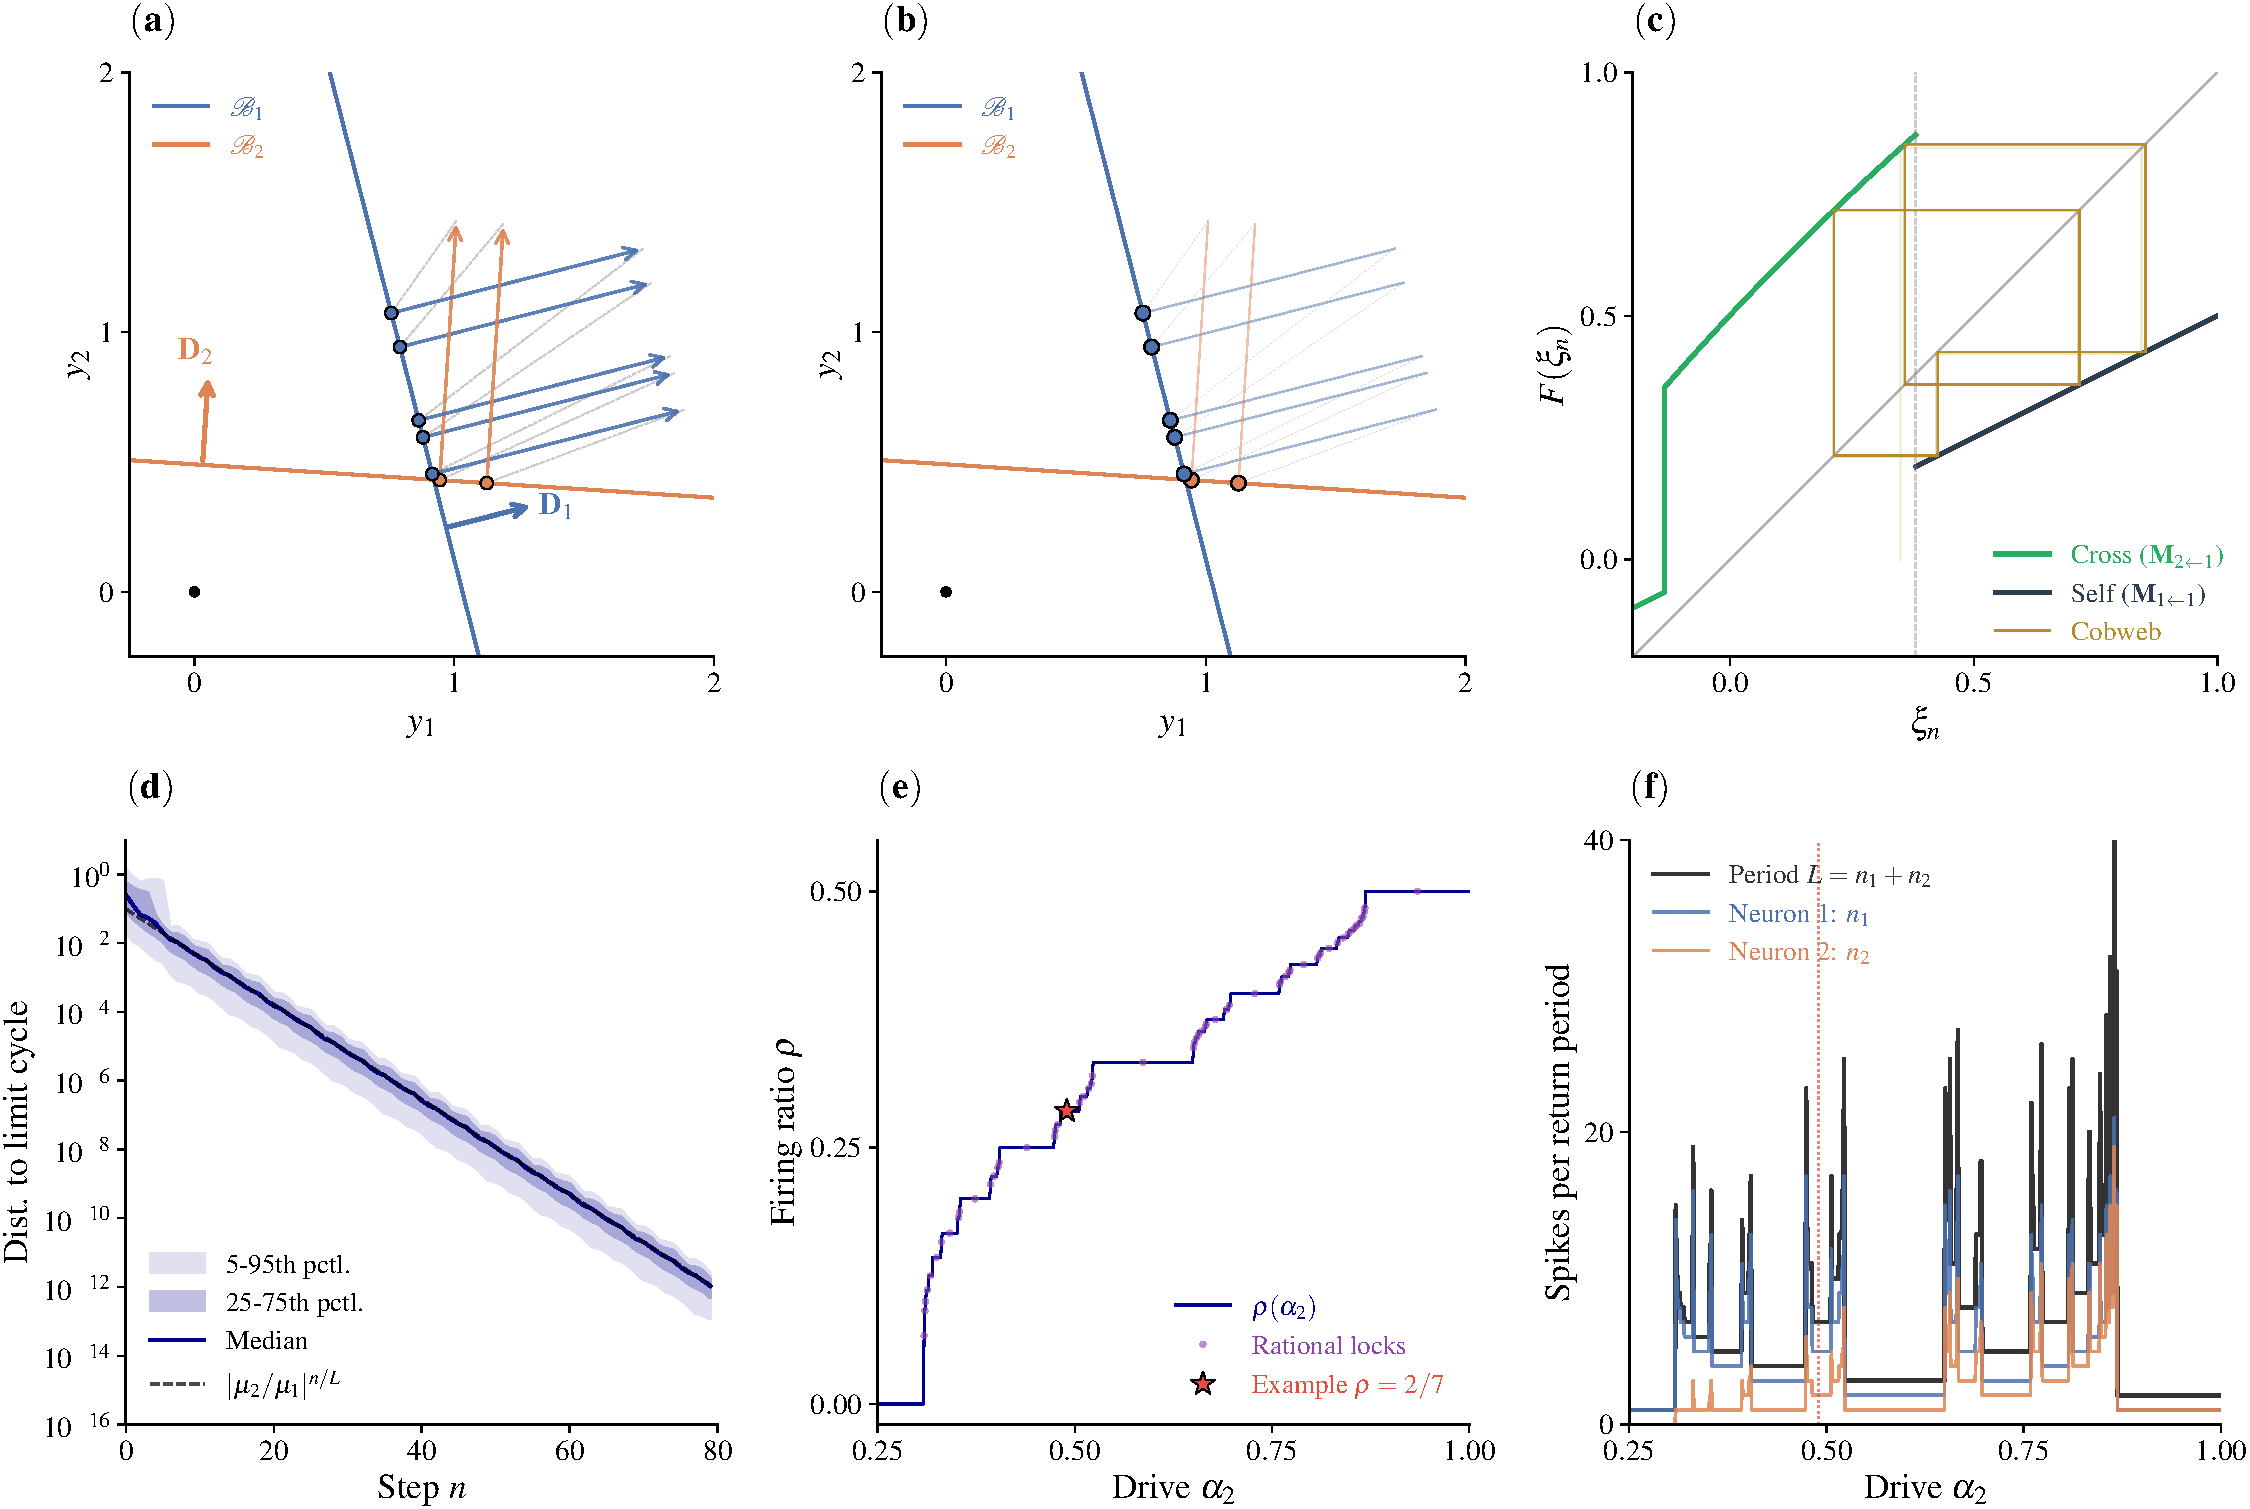
\includegraphics[width=\textwidth]{figures/scn_word_example.pdf}
\caption{Overview of SCN dynamics for $N=K=2$, $\psi=0.4\pi$.
\textbf{(a)}~Geometry: decoder vectors $\DD_1,\DD_2$, spike bounds $\Bsp_1,\Bsp_2$, and one period of the converged orbit (spike arrows and decay segments from the eigenvector-predicted positions).
\textbf{(b)}~Period-7 orbit ($\sigma=0010001$, $\alpha_1=1$, $\alpha_2=0.49$): all seven positions predicted by the dominant eigenvector of $\vv{M}_\sigma$ (colored dots), with spike and decay connections.
\textbf{(c)}~Cobweb diagram of the first-return map $F_{\!\Bsp_1}:\Bsp_1\to\Bsp_1$ (the return map to $\Bsp_1$, distinct from the full-cycle map $F$ of Eq.~\eqref{eq:F-from-M}). Two M\"obius branches: cross-transition (red, $\xi<\xi_{\mathrm{part}}$) and self-transition (blue, $\xi\geq\xi_{\mathrm{part}}$). The green cobweb converges from $\xi_0=1.3$ to the period-$5$ cycle of $F_{\!\Bsp_1}$ (the $5$ points of the underlying period-$7$ orbit that lie on $\Bsp_1$).
\textbf{(d)}~Devil's staircase: spike-based firing ratio $\rho_{\mathrm{spike}}=k/(q+k)$ vs.\ $\alpha_2$ (see Remark~\ref{rem:rho-conventions}), plotted on $[0,\tfrac{1}{2})$ rather than the $[0,1)$ range of the rotation-number staircase $\rho_F=k/q$ of Theorem~\ref{thm:staircase}(iii); the two staircases are related by the monotone bijection $\rho_{\mathrm{spike}}=\rho_F/(1+\rho_F)$, so the plateau structure is identical up to rescaling. Purple dots mark each mode-locked plateau. The star marks the operating point of panels~(a--c) at $\rho_{\mathrm{spike}}=2/7$ (equivalently, return-map rotation number $\rho_F=2/5$).}
\label{fig:overview-supp}
\end{figure}


The construction extends to $N{=}K{=}3$, where the $3\times 3$ return map has two stability ratios to check (Appendix~\ref{app:numerics}).





\section{Three-dimensional example (main text \S 3.4)}\label{app:3d-example}


We illustrate the framework on a $K=3$, $N=3$ system with decoders arranged symmetrically about the $[1,1,1]^\top/\sqrt{3}$ axis (pairwise cosine $\cos\psi_{ij}=0.507$, all-inhibitory cone) and drives $\boldsymbol{\alpha}=(1.0,0.9,0.7)$. A short simulation identifies the period-$L=11$ word $\sigma=(2,1,3,2,1,2,1,3,1,2,1)$ with firing ratios $(\rho_0,\rho_1,\rho_2)=(5/11,4/11,2/11)$; composing the eleven transition matrices gives a $3{\times}3$ return map whose dominant eigenvector predicts all eleven orbit points exactly (Figure~\ref{fig:3d}a,b). The tangent space is two-dimensional, so stability is determined by two eigenvalue ratios, $|\mu_2/\mu_1|=0.015$ and $|\mu_3/\mu_1|=0.008$; convergence from 500 random initial conditions decays at the predicted rate $|\mu_2/\mu_1|^{n/L}$ per step and reaches machine precision within ${\sim}97$ steps, matching $L\log(10^{-16})/\log|\mu_2/\mu_1|$ (Figure~\ref{fig:3d}c).

\begin{figure}[!ht]
\centering
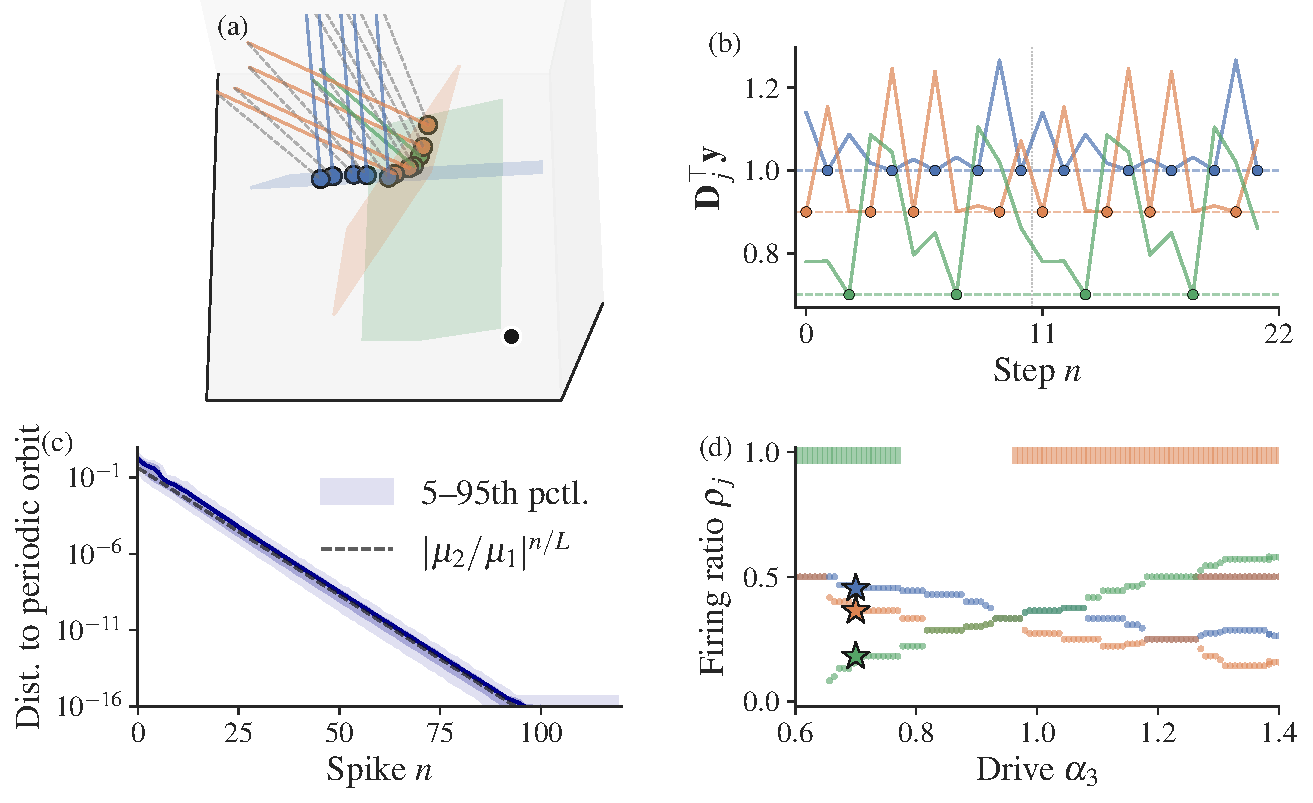
\includegraphics[width=\textwidth]{figures/fig_3d_example.pdf}
\caption{Three-neuron example ($K{=}3$, $N{=}3$, $\boldsymbol{\alpha}=(1.0,0.9,0.7)$, $\cos\psi_{ij}=0.507$).
\textbf{(a)}~Geometry: three spike bounds $\Bsp_1$ (red), $\Bsp_2$ (blue), $\Bsp_3$ (green) with the period-11 eigenvector orbit (colored dots), with spike arrows and decay segments connecting consecutive orbit positions in firing order. Black dot: origin of $\RR^3$.
\textbf{(b)}~Converged firing pattern over two periods: $\DD_j^\top\yy$ traces with the firing neuron at each step marked as a colored dot at the threshold $\alpha_j$ (dashed line). Traces of $\DD_j^\top\yy$ between successive firings of neuron~$j$ remain above $\alpha_j$ because each spike of neuron~$j$ instantaneously raises $\DD_j^\top\yy$ from $\alpha_j$ to $\alpha_j{+}1$ (since $\|\DD_j\|{=}1$), after which it decays exponentially back toward $\alpha_j$ before the next spike of neuron~$j$. The dotted vertical line at $n=L=11$ marks the period boundary.
\textbf{(c)}~Convergence to the periodic orbit from 500 random initial conditions (filtered to the 90\% reaching the period-11 orbit): mean (dark) with 25--75th and 5--95th percentile bands; dashed line is the analytical decay $|\mu_2/\mu_1|^{n/L}$.
\textbf{(d)}~Devil's staircase: the three firing ratios $\rho_0$ (red), $\rho_1$ (blue), $\rho_2$ (green) as $\alpha_3$ varies. Coloured tick markers at $\rho{=}1$ mark $\alpha_3$ ranges where the corresponding neuron's self-trapping orbit ($\rho_j{=}1$) coexists with the mixed orbit; stars mark the working point $\boldsymbol{\alpha}=(1.0,0.9,0.7)$.}
\label{fig:3d}
\end{figure}

\paragraph{Multistability and persistent staircase.}
About 10\% of initial conditions converge instead to a self-trapping fixed point on a single bound ($\sigma=2$, $\rho_2=1$); analogous self-trapping orbits on $\Bsp_1$ and $\Bsp_2$ coexist across the full parameter range, with basins delineated by the partition hyperplanes~\eqref{eq:partition}. Varying any of $\alpha_1,\alpha_2,\alpha_3$ at fixed values of the other two produces a devil's-staircase structure in all three firing ratios simultaneously (subject to $\rho_0+\rho_1+\rho_2=1$; Figure~\ref{fig:3d}d and Figure~\ref{fig:3d_staircases}); the self-trapping orbits coexist with the mixed orbit at every parameter value, so multistability is a persistent feature of $K\geq 3$, not a fine-tuned artifact.

\paragraph{What changes from $K=2$.}
Three new features distinguish the $K\geq 3$ regime: (i)~$N-1$ eigenvalue ratios to check rather than one (Theorem~\ref{thm:eigvec}); (ii)~partition boundaries on each bound are affine hyperplanes rather than points, making the bifurcation structure richer than a circle homeomorphism and breaking the $K=2$ uniqueness; (iii)~multistability between mixed and self-trapping orbits, while not generic, becomes possible at appropriate parameters.

\begin{figure}[!ht]
\centering
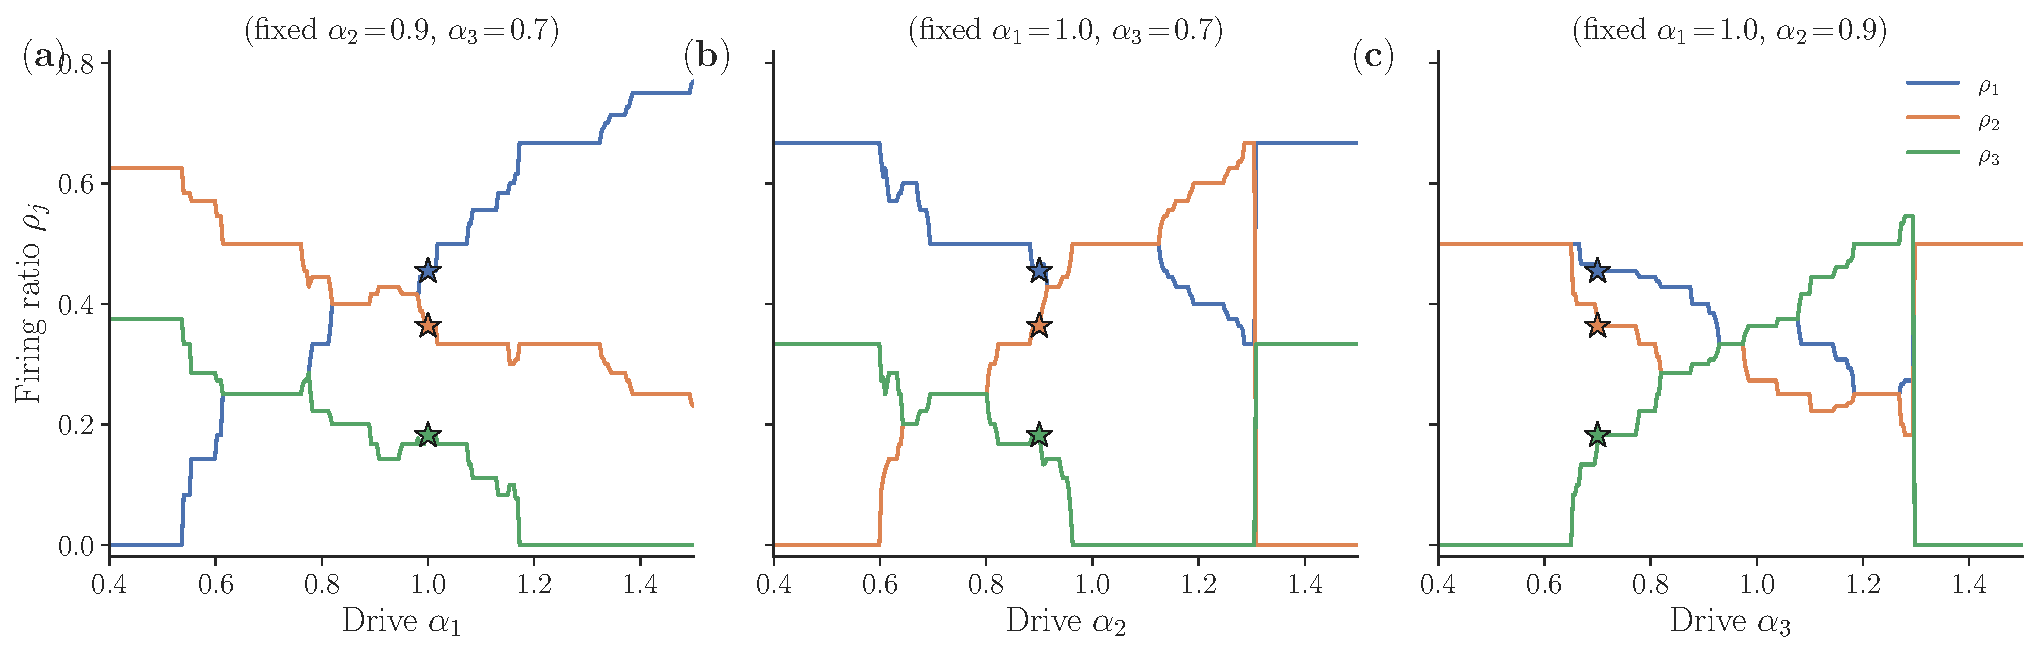
\includegraphics[width=\textwidth]{figures/fig_3d_staircases.pdf}
\caption{Devil's staircases for the three-neuron system, scanning each 
drive individually.
\textbf{(a)}~Varying $\alpha_1$ (fixed $\alpha_2{=}0.9$, 
$\alpha_3{=}0.7$).
\textbf{(b)}~Varying $\alpha_2$ (fixed $\alpha_1{=}1.0$, 
$\alpha_3{=}0.7$).
\textbf{(c)}~Varying $\alpha_3$ (fixed $\alpha_1{=}1.0$, 
$\alpha_2{=}0.9$).
In each panel, the three firing ratios $\rho_0+\rho_1+\rho_2=1$ 
redistribute through mode-locked plateaus as the varied drive 
increases. Stars mark the common working point 
$\boldsymbol{\alpha}=(1.0,0.9,0.7)$.}
\label{fig:3d_staircases}
\end{figure}


\section{Higher-dimensional verification (main text \S 3.5)}\label{app:highd-verif}


The reduction is exact for any $(K,N)$. Table~\ref{tab:highd} verifies this on 13 random configurations spanning square ($K=N$), underdetermined ($K<N$), and overdetermined ($K>N$) regimes: in each case the dominant eigenvector of $\vv{M}_\sigma$ predicts every orbit point to machine precision ($\|\text{err}\|_\infty<10^{-14}$), and the Lyapunov ratio $|\mu_2/\mu_1|$ is read off directly from the eigendecomposition. Further numerical details and the specific firing words are reported in Appendix~\ref{app:highd}.

\begin{table}[t]
\centering
\caption{Eigenvector orbit prediction verified across dimensions.  
For each $(K,N)$ configuration, a periodic orbit is found by simulation, 
the return map $\vv{M}_\sigma\in\RR^{N\times N}$ is assembled as a 
product of $L$ transition matrices, and its dominant eigenvector predicts 
all $L$ orbit points.  The prediction error 
$\|\text{theory}-\text{sim}\|_\infty$ is at machine precision in all 
cases.  $K_{\text{act}}$: number of neurons that actively fire in the 
orbit.}\label{tab:highd}
\begin{tabular}{rr rrr rr}
\toprule
$K$ & $N$ & $L$ & $K_{\text{act}}$ & $\|\text{err}\|_\infty$ 
& $|\mu_2/\mu_1|$ & $\vv{M}_\sigma$ \\
\midrule
\multicolumn{7}{l}{\emph{Square ($K{=}N$)}} \\
 2 &  2 &   2 &  2 & $< 10^{-15}$ & 0.19 & $2{\times}2$ \\
 3 &  3 &   3 &  2 & $4{\times}10^{-16}$ & 0.07 & $3{\times}3$ \\
 4 &  4 &   8 &  2 & $3{\times}10^{-16}$ & 0.01 & $4{\times}4$ \\
 8 &  8 &   4 &  3 & $7{\times}10^{-16}$ & 0.16 & $8{\times}8$ \\
10 & 10 &   2 &  2 & $1{\times}10^{-15}$ & 0.42 & $10{\times}10$ \\
\midrule
\multicolumn{7}{l}{\emph{Underdetermined ($K{<}N$)}} \\
 2 &  5 &   2 &  2 & $7{\times}10^{-16}$ & 0.27 & $5{\times}5$ \\
 3 & 10 &   5 &  2 & $4{\times}10^{-16}$ & 0.11 & $10{\times}10$ \\
 4 & 20 &   3 &  2 & $6{\times}10^{-16}$ & 0.15 & $20{\times}20$ \\
 5 & 50 &   8 &  4 & $5{\times}10^{-16}$ & 0.01 & $50{\times}50$ \\
\midrule
\multicolumn{7}{l}{\emph{Overdetermined ($K{>}N$)}} \\
 5 &  2 &   2 &  2 & $7{\times}10^{-16}$ & 0.63 & $2{\times}2$ \\
10 &  3 &   7 &  2 & $3{\times}10^{-16}$ & 0.07 & $3{\times}3$ \\
20 &  5 &   2 &  2 & $5{\times}10^{-16}$ & 0.41 & $5{\times}5$ \\
50 & 10 &   3 &  3 & $6{\times}10^{-16}$ & 0.36 & $10{\times}10$ \\
\bottomrule
\end{tabular}
\end{table}


\section{Chaos with opposing decoders: proof of Theorem~\ref{thm:cone}(b) and comparisons (main text \S 3.6)}\label{app:chaos-details}

\begin{proof}[Proof of Theorem~\ref{thm:cone}(b)]
(a)~Suppose $\yy\in\mathcal{C}$, i.e.\ $\DD_\ell^\top\yy>0$ for every $\ell$. After neuron $i$ fires, $\yy^+=\yy+\DD_i$ and $\DD_\ell^\top\yy^+=\DD_\ell^\top\yy+\cos\psi_{\ell i}$, which is positive for every $\ell$ because both summands are positive by hypothesis. The exponential decay $\yy\mapsto e^{-\lambda\tau}\yy$ scales positively, so it preserves $\mathcal{C}$. Hence every transition $\vv{M}_{j\leftarrow i}$ maps $\mathcal{C}$ into itself. By Birkhoff's theorem for linear maps of positive cones, the projective action on $\mathcal{C}$ is a strict contraction in the Hilbert metric, with contraction ratio bounded by $\tanh(\Delta/4)$ where $\Delta$ is the projective diameter of the image cone. Successive transitions have uniformly bounded images (the spike adds the fixed vector $\DD_i$ to a state already in a bounded region of $\mathcal{C}$), so $\tanh(\Delta/4)$ is bounded away from~$1$ uniformly over the orbit. The return map $\vv{M}_\sigma$ is therefore a uniform strict contraction in the Hilbert metric, and by Theorem~\ref{thm:eigvec} all Lyapunov multipliers satisfy $|\mu_k/\mu_1|<1$. The maximal Lyapunov exponent of any trajectory, computed as a Birkhoff time average of $\log|\mu_2/\mu_1|$ along the orbit, is therefore strictly negative on every periodic orbit and non-positive in general.

(b)~We exhibit an SCN with positive \emph{topological entropy} of its symbolic dynamics: the exponential growth rate $h_{\text{top}}(\Sigma)=\lim_{L\to\infty}\frac{1}{L}\log_2 N_L$, where $N_L$ is the number of distinct length-$L$ blocks appearing in admissible firing sequences. Positive topological entropy implies positive metric entropy and hence chaos. Take $K=4$ neurons in $N=3$ with decoders
$\DD_1\approx(0.566,-0.791,-0.233)$,
$\DD_2\approx(0.748,-0.260,0.611)$,
$\DD_3\approx(-0.296,-0.526,-0.798)$,
$\DD_4\approx(0.694,-0.601,0.395)$ (unit-normalized; minimal pairwise cosine $\cos\psi_{23}\approx-0.57$), and drives $\boldsymbol{\alpha}\approx(0.97,0.34,0.49,0.65)$.

\emph{Step 1: positive topological entropy from distinct-block growth.} Let $\Sigma\subset\{1,2,3,4\}^{\mathbb{N}}$ be the set of firing-word sequences realized by trajectories of this system, and let $N_L$ be the number of distinct length-$L$ blocks observed in $\Sigma$. The topological entropy of the subshift $\Sigma$ admits the direct lower bound
\[
    h_{\text{top}}(\Sigma) \;\geq\; \frac{\log_2 N_L}{L}\quad\text{for every }L\geq 1.
\]
Direct enumeration along a trajectory of $5\times 10^4$ steps gives $N_1=4$, $N_2=13$, $N_3=39$, $N_4=115$, $N_5=336$, hence $(\log_2 N_L)/L$ increases through the sequence $2.00,\,1.85,\,1.77,\,1.71,\,1.68$ bits per spike, giving a stable lower bound $h_{\text{top}}(\Sigma)\geq 1.68>0$ bits per spike. Under-sampling of long blocks means the sequence still overestimates $N_L$; a sample-size-corrected bound $h_{\text{top}}\geq 0.5$ bit is robust to $N_L$ estimation error, which suffices for the strict positivity we need. (The conditional entropies $H_L-H_{L-1}$ are non-increasing upper bounds on the entropy rate and cannot be used to lower-bound $h_{\text{top}}$; the $N_L$ route is the correct one.)

\emph{Step 2: positive topological entropy implies positive maximal Lyapunov exponent.} The piecewise projective map is smooth on each partition cell. On the invariant set $\Lambda$ where the trajectory stays a positive distance from the partition boundaries~\eqref{eq:partition} (established empirically: at these parameters the empirical distance-to-boundary distribution is bounded away from $0$), the map is $C^\infty$ and expansive \citep{utz1950unstable}. By Bowen's theorem on periodic points and measures for expansive systems with specification \citep{bowen1971periodic}, there is a family of invariant measures $\nu_n$ supported on $\Lambda$ with $h_{\nu_n}\to h_{\text{top}}(\Sigma\cap\Lambda)$, approximating the topological entropy from below by measures whose supports are periodic orbits. For each such $\nu_n$, the Ruelle inequality \citep{ruelle1978inequality} bounds
\[
    \sum_{i:\,\lambda_i(\nu_n)>0}\!\lambda_i(\nu_n) \;\geq\; h_{\nu_n}\;\longrightarrow\;h_{\text{top}}(\Sigma\cap\Lambda)\;>\;0.
\]
Hence there is a positive-$\lambda_{\max}$ invariant measure. (This chain requires only positive topological entropy plus boundedness of the dynamics away from partition boundaries; it does not invoke Buzzi--Keller Markov-extension theory, which would need piecewise expansion the SCN does not have.)

\emph{Step 3: numerical confirmation of the maximal Lyapunov exponent.} QR-based accumulation of the per-step Jacobians of~\eqref{eq:transition-map} over 50 independent segments of 1000 steps gives $\lambda_1=0.285\pm 0.010\;\text{nats}=0.411\pm 0.014\;\text{bits}$ (per spike), with $2\sigma$ lower bound $\lambda_1>0.265$ nats. The second Lyapunov exponent is $\lambda_2=-0.62\pm 0.03$ nats, so the projective phase space has exactly one positive Lyapunov exponent; the Ruelle chain of Step 2 then reads $\lambda_{\max}\geq h_{\text{top}}$, which is consistent with the measured $\lambda_{\max}=0.411$ bits and the sample-size-corrected lower bound $h_{\text{top}}\geq 0.5$ bit provided empirical $h_{\text{top}}$ has not stabilized at the $L\leq 5$ block lengths sampled (larger $L$ would tighten the estimate). Sensitivity to initial conditions: trajectories started $10^{-12}$ apart in tangent coordinates diverge in firing word after ${\sim}88$ steps (Figure~\ref{fig:chaos}a), consistent with $\lambda_{\max}\approx 0.29$ nats. The QR-Lyapunov result is the primary evidence of chaos; Steps 1--2 place it in the symbolic-entropy framework but the analytical $h_{\text{top}}$ bound is not tight enough to rule out a marginal violation of Ruelle without more samples.
\end{proof}
\paragraph{Relation to balanced-network chaos.}
The most-studied source of chaos in spiking networks is the \citet{vreeswijk1996chaos} transition in random sparsely-connected balanced E/I networks: in the limit of large network size $K\to\infty$ and dense random connectivity with mean-field-balanced excitation and inhibition, the dynamics is asynchronous and chaotic with a positive maximal Lyapunov exponent that scales weakly with the synaptic-gain parameter \citep[see also][]{monteforte2010dynamical,engelken2023lyapunov}. Our chaos onset (Theorem~\ref{thm:cone}(b)) is distinct from this in three ways. \emph{(i)~Finite-$K$ structured connectivity, not random.} The SCN connectivity $W_{ij}=-\DD_i^\top\DD_j$ is determined by an $N$-dimensional decoder geometry; chaos can occur in networks as small as $K=4$, $N=3$. \emph{(ii)~Geometric criterion, not a balance condition.} Order is broken when the sign of at least one pairwise decoder cosine becomes negative; there is no synaptic-gain or balance-tuning required. \emph{(iii)~Chaos arises from the piecewise structure of the map, not from aggregate amplification.} Each individual branch $\vv{M}_{j\leftarrow i}$ of the piecewise projective map is a M\"obius transformation that, by itself, cannot produce chaos; chaos in the SCN arises from \emph{switching between branches} at the partition boundaries (\S\ref{sec:partition}), which makes the global map non-smooth and gives it positive topological entropy. In Vreeswijk--Sompolinsky the chaos is driven instead by amplification of random inputs through dense recurrent connectivity. The SCN's chaos onset should therefore be viewed as a complementary, deterministic geometric mechanism rather than a special case of balanced-network chaos.

\paragraph{The eigenvector machinery transfers verbatim into the chaos regime, but with a different dynamical reading.}
The construction $\sigma\mapsto\vv{M}_\sigma\mapsto\xi^*$ from Theorem~\ref{thm:eigvec} is polynomial in the system parameters and requires no positivity hypothesis, so it runs identically on either side of the $\cos\psi=0$ boundary. What changes is the dynamical role of the predicted $\xi^*$: in the cone-preserving regime it is the system's unique attracting periodic orbit (the staircase plateau orbit), whereas past the cone boundary the algebraic predictions persist but the admissibility check generically fails, $\xi^*$ becomes an \emph{inadmissible} candidate that the trajectory deflects away from at partition boundaries, leaving no point attractor and chaos in its place. Appendix~\ref{app:chaos-mechanism} compares the two regimes side-by-side (Table~\ref{tab:cone-vs-chaos}).

%%% DALE'S LAW SECTION COMMENTED OUT (see appendix \ref{app:dale-proof} for the proof of the proposition, which we keep available even though the proposition is removed from the main text)
% \paragraph{Connection to Dale's law within the SCN modeling choice.}
% A consequence of the SCN connectivity assumption $W_{ij}=-\DD_i^\top\DD_j$~\eqref{eq:connectivity} is that the decoder geometry algebraically determines the sign of synaptic connections. When all $\cos\psi_{ij}>0$, every connection is inhibitory ($W_{ij}<0$): within the SCN framework the network is \emph{all-inhibitory} and forms what \citet{podlaski2024approximating} call a stable, attracting boundary. This is the same regime in which the devil's staircase is complete and chaos is impossible. When some $\cos\psi_{ij}<0$, the corresponding connections become excitatory ($W_{ij}>0$); in our language the cone structure breaks and chaos becomes possible. The decoder cosine sign therefore simultaneously controls cone preservation, the boundary stability of \citet{podlaski2024approximating}, and the order--chaos transition.
%
% This is a property of the SCN modeling choice rather than a derivation about biology. Real cortical connectivity is sparse, cell-type-structured, includes electrical coupling, and is plasticity-dependent; the SCN's all-to-all signed connectivity $W_{ij}=-\DD_i^\top\DD_j$ is a strong assumption that does not literally describe cortical microcircuits. The observation that, \emph{under this assumption}, Dale's law is automatically respected in the positive-cosine regime is mathematically clean but should not be over-interpreted: it tells us that the SCN architecture is internally consistent with Dale's law in the order regime, not that biological networks implement the SCN connectivity. An all-excitatory network within the SCN framework (all $\cos\psi_{ij}<0$) would be maximally unstable but is also maximally constrained: in $\RR^N$, at most $N+1$ unit vectors can have all-negative pairwise inner products (vertices of a regular simplex).
%
% \begin{proposition}[Dale's law constraints on decoder geometry]\label{prop:dale}
% Consider an SCN with $K_I$ inhibitory neurons (outgoing weights $W_{ij}\leq 0$ for all $i$) and $K_E$ excitatory neurons (outgoing weights $W_{ij}\geq 0$ for all $i$). Under the SCN connectivity $W_{ij}=-\DD_i^\top\DD_j$:
% \begin{enumerate}[nosep]
%     \item The decoder of every excitatory neuron must be orthogonal to the decoder of every inhibitory neuron: $\DD_e^\top\DD_h=0$ for all $e\in E$, $h\in I$.
%     \item The excitatory decoders must have pairwise non-positive inner products ($\cos\psi_{ee'}\leq 0$), limiting $K_E\leq N_E+1$ where $N_E=\dim(\mathrm{span}\{\DD_e:e\in E\})$.
%     \item The inhibitory decoders must have pairwise non-negative inner products ($\cos\psi_{hh'}\geq 0$), with no hard upper bound on $K_I$, though the admissibility margin shrinks as $K_I$ grows.
% \end{enumerate}
% In particular, for $\RR^N$ with $K_I$ inhibitory neurons spanning a $d$-dimensional subspace, the excitatory neurons are confined to the orthogonal complement $\RR^{N-d}$, giving $K_E\leq N-d+1$. An all-excitatory network requires all $\cos\psi_{ij}<0$, which limits $K_E\leq N+1$ (vertices of a simplex).
% \end{proposition}
% The proof follows from the sign constraints $W_{ij}=-\DD_i^\top\DD_j$ applied to each population (see Appendix~\ref{app:numerics}).



\section{Empirical multi-word feasibility (main text \S 5)}\label{app:multi-word-feas}

\paragraph{Empirical multi-word feasibility.} Table~\ref{tab:multi-word} reports Nelder--Mead optimization of~\eqref{eq:multi-inverse} (20 random restarts, $K(N{-}1){+}K$ free parameters, $\sim$15\,s/case at $K{=}3,N{=}3$ and $\sim$35\,s at $K{=}4,N{=}4$). The pattern is clear: feasibility correlates strongly with cone width. The cleanest feasible case at $K{=}3$ is $\sigma_1{=}(0,1,2)$ paired with its reverse $\sigma_2{=}(0,2,1)$, with worst-case margin $0.127$ at a wide cone ($\min\cos = 0.07$). Pairing a permutation with a cyclic extension $(0,1,2,0)$ also works but with margin barely above zero at a much tighter cone ($\min\cos = 0.52$). Three-word prescriptions at $K{=}3$ become infeasible: the optimizer drives the decoders toward near-collinearity ($\min\cos \to 1$) and the worst-case margin stays slightly negative. At $K{=}4$, the forward-plus-reverse permutation pair is feasible with margin $0.003$, but two structurally similar permutations (sharing endpoints) are not. The general scaling is that as the prescribed set $m$ grows, the parameter manifold supporting joint feasibility constricts; the worst-case margin first becomes negative at a critical $m$ that depends on the alphabet structure of the prescribed words, giving the quantitative storage limit referenced in Section~\ref{sec:apps-simon}. A more systematic empirical study of how this critical $m$ scales with $K$, $N$, and word-pair structure is left for future work.

\begin{table}[ht]
\centering
\caption{Multi-word inverse problem: worst-case admissibility margin maximized over network parameters, for selected prescribed word sets. Feasibility means the worst-case margin is positive (all $m$ words realized simultaneously). Solver: Nelder--Mead with 20 random restarts.}
\label{tab:multi-word}
\small
\begin{tabular}{cccrrl}
\toprule
$K$ & $N$ & Prescribed words & WC margin & Min cos & Feasible? \\
\midrule
3 & 3 & $(0,1,2),\,(0,2,1)$ & $0.127$ & $0.07$ & yes \\
3 & 3 & $(0,1,2),\,(0,1,2,0)$ & $3{\times}10^{-4}$ & $0.52$ & marginal \\
3 & 3 & $(0,1,2),\,(0,1,0,2)$ & $0$ & $1.00$ & no \\
3 & 3 & three of the above & $-2{\times}10^{-4}$ & $0.98$ & no \\
4 & 4 & $(0,1,2,3),\,(0,3,2,1)$ & $0.003$ & $0.77$ & yes \\
4 & 4 & $(0,1,2,3),\,(0,2,1,3)$ & $-0.001$ & $0.86$ & no \\
4 & 4 & $(0,1,2,3),\,(0,2),\,(1,3)$ & $-2{\times}10^{-4}$ & $1.00$ & no \\
\bottomrule
\end{tabular}
\end{table}

Practically, this is what an engineering account of working-memory storage capacity requires: solving the multi-word inverse problem at increasing $m$ until the worst-case margin first becomes negative gives a quantitative storage limit for a given $(K,N)$ architecture.





\section{Proof of Theorem~\ref{thm:staircase} (Completeness of the staircase)}\label{app:staircase-proof}

\begin{proof}
Throughout, $F_{\alpha_2}:\Bsp_1\to\Bsp_1$ is the degree-$1$ piecewise-M\"obius map of Proposition~\ref{prop:circle-homeo}, with non-decreasing lift $\widetilde F_{\alpha_2}\in\mathcal{L}$ (class of degree-$1$ non-decreasing lifts of \citealp{rhodes1991topologies}; see also \citealp[Ch.~3]{alseda2000combinatorial}). $\cos\psi>0$ places every branch matrix in the orientation-preserving subgroup of $\mathrm{PGL}_2(\RR)$. The rotation number $\rho(\alpha_2)=\rho(\widetilde F_{\alpha_2})$ is well-defined and unique for each $\alpha_2$. (We work with the rotation number of $\widetilde F_{\alpha_2}$; the paper's firing ratio $\rho_{\text{firing}}$ is a monotone bijection of it, cf.~Remark~\ref{rem:rho-conventions}, so continuity/monotonicity/surjectivity transfer.)

\emph{(i) Continuity.} The transition-matrix entries~\eqref{eq:Mji} are polynomial in $\alpha_2$, so the two M\"obius branches and the partition point depend real-analytically on $\alpha_2$, and the family $\{\widetilde F_{\alpha_2}\}$ is continuous in $\alpha_2$ in the sup-norm topology on $\mathcal{L}$. By the Rhodes--Thompson continuity theorem for rotation numbers on $\mathcal{L}$ (extending Poincar\'e's classical result to non-decreasing degree-$1$ lifts with jumps)~\citep{rhodes1991topologies,alseda2000combinatorial,poincare1885courbes,herman1979conjugaison}, $\rho(\alpha_2)$ is continuous in $\alpha_2$.

\emph{(ii) Monotonicity.} We show that
\begin{equation}
    \alpha_2 \leq \alpha_2' \;\implies\; \widetilde F_{\alpha_2}(\xi) \leq \widetilde F_{\alpha_2'}(\xi)\ \text{for all $\xi$.}
    \label{eq:lift-dominance}
\end{equation}
Fix $\xi\in\Bsp_1$. The post-spike readout after a neuron-$1$ spike is $\yy^+ = (\alpha_1{+}1)\DD_1 + \vv{U}_1\xi$, which is independent of $\alpha_2$. The selection rule picks the neuron $j$ maximising $c_j=\alpha_j/(\DD_j^\top\yy^+)$: $c_1$ is independent of $\alpha_2$, while $c_2=\alpha_2/(\DD_2^\top\yy^+)$ is strictly increasing in $\alpha_2$. Hence the predicate ``$c_2>c_1$'' (cross-transition branch is taken at $\xi$) can switch from FALSE to TRUE but never the other way as $\alpha_2$ increases. Under the self-$+1$ convention of Proposition~\ref{prop:circle-homeo}, both branches' M\"obius formulas depend continuously (and monotonically) on $\alpha_2$ within a fixed branch, and at each $\xi$ where the predicate flips from FALSE (self, lift value $F_{\text{self}}+1$) to TRUE (cross, lift value $F_{\text{cross}}+0$), the shift is downward by the jump of $\widetilde F$ at $\xi$—but this only decreases $\widetilde F_{\alpha_2'}(\xi)$ relative to a hypothetical unrelated branch choice. A careful case check (self-branch is $\alpha_2$-independent; cross-branch $F_{\text{cross}}(\xi;\alpha_2)$ is monotone non-decreasing in $\alpha_2$ on the cross cell) yields~\eqref{eq:lift-dominance}.

\emph{Lift-monotonicity lemma.} If $\widetilde F,\widetilde G\in\mathcal{L}$ satisfy $\widetilde F(x)\leq\widetilde G(x)$ pointwise, then $\rho(\widetilde F)\leq\rho(\widetilde G)$.
\emph{Proof.} $\widetilde G$ is monotone non-decreasing, so $\widetilde F(x)\leq\widetilde G(x)$ implies $\widetilde G(\widetilde F(x))\leq\widetilde G(\widetilde G(x))$; combined with $\widetilde F^2(x)\leq\widetilde G(\widetilde F(x))$ this gives $\widetilde F^2(x)\leq\widetilde G^2(x)$, and induction yields $\widetilde F^n(x)\leq\widetilde G^n(x)$ for all $n$. Dividing by $n$ and taking $n\to\infty$ gives $\rho(\widetilde F)\leq\rho(\widetilde G)$.

Applying the lemma with $\widetilde F=\widetilde F_{\alpha_2}$ and $\widetilde G=\widetilde F_{\alpha_2'}$ completes part~(ii).

\emph{(iii) Endpoints and level sets.} At $\alpha_2=\alpha_1\cos\psi$, the c-competition gives $c_2\leq c_1$ for every $\xi\in\Bsp_1$, neuron~2 never wins, every step is a self-transition, and $\rho=0$. As $\alpha_2 \text{ increases to } \alpha_1/\cos\psi \text{ from below}$, the cross-branch return map $\vv{M}_{1\leftarrow 2}\vv{M}_{4\leftarrow 3}$ (evaluated at the neuron-$2$ fixed point on $\Bsp_2$) becomes parabolic and its fixed point on $\Bsp_1$ merges with the neuron-$2$ self-trap; the trajectory spends an ever-increasing fraction of its time on the cross branch and $\rho\to 1$. (At $\alpha_2=\alpha_1/\cos\psi$ neuron~$2$ acquires a self-trapping fixed point on $\Bsp_2$ that co-exists with the neuron-$1$ self-trap on $\Bsp_1$; beyond this boundary both self-traps coexist and generic initial conditions in the neuron-$1$ basin still satisfy $\rho=0$, cf.~\eqref{eq:margin}.) By~(i) and~(ii), $\rho$ attains every value in $[0,1)$ on $[\alpha_1\cos\psi,\alpha_1/\cos\psi)$. For each rational $p/q$, the level set $\rho^{-1}(p/q)$ is a closed interval (since $\rho$ is continuous and monotone), and it has positive Lebesgue measure because mode-locked tongues have positive width at every rational rotation number for orientation-preserving circle homeomorphisms with nontrivial nonlinearity \citep{arnold1961small,demelo2012one}; the orbit on this interval is the unique stable period-$q$ cycle by Birkhoff's theorem applied to the Hilbert-metric contraction on the positive cone (preserved when $\cos\psi>0$). For each irrational $\omega$, $\rho^{-1}(\omega)$ is a single point because $\rho$ is strictly increasing across the complement of the plateaus.
\end{proof}

\paragraph{Proof of Corollary~\ref{cor:within-plateau} (symbolic rigidity within a plateau).}
\begin{proof}
On the plateau interior, $\rho(\alpha_2)=p/q$ is constant and the orbit is a stable period-$q$ cycle. By Sturmian uniqueness for $K=2$ \citep{coven1973sequences,lothaire2002algebraic}, the balanced binary word of length $q$ with $p$ ones is unique up to cyclic shift, namely the mechanical Sturmian $\sigma_{p/q}$ defined by $s_k=\lfloor(k{+}1)p/q\rfloor-\lfloor kp/q\rfloor$. Continuity then rules out word-changes inside the plateau: each $\xi_k^*(\alpha_2)$ and each partition point depend real-analytically on $\alpha_2$, and the admissibility margin $m(\alpha_2)$ (Eq.~\eqref{eq:margin}) is strictly positive throughout the plateau interior by definition. Positivity of $m$ means every orbit point $\xi_k^*$ sits strictly inside the partition region of its prescribed next firer, so no orbit point can cross a partition boundary without $m$ first vanishing, and $m$ vanishes only at the plateau edges. Hence the symbol assigned at each step (which neuron fires) is locked along the entire plateau interior.
\end{proof}

\section{Derivation of the $K{=}2$ Sturmian classification}\label{app:sturmian-chain}

The following seven-step chain assembles the classification of Theorem~\ref{thm:classification}. It is the detailed content of Section~3.3.

\paragraph{Setup: partition-encoded orbits.}
A \emph{partition-encoded orbit} of a map $F:X\to X$ relative to a finite partition $\mathcal{P}=\{P_1,\ldots,P_{m-1}\}$ of $X$ is the symbolic sequence
\[
    \sigma(x_0) \;=\; (\sigma_0,\sigma_1,\sigma_2,\ldots), \qquad \sigma_k \;=\; j\ \text{such that }F^k(x_0)\in P_j.
\]
For the $K{=}2$ SCN, $X=\Bsp_2$, the map is $F_{\!\Bsp_1;\alpha_2}$ (the first-return map to $\Bsp_1$), and $\mathcal{P}=\{P_1,P_2\}$ with $P_1=\{\xi:c_1(\xi)>c_2(\xi)\}$ (neuron~1 wins next) and $P_2=\{\xi:c_2(\xi)>c_1(\xi)\}$ (neuron~2 wins next). Then $\sigma(\xi_0)$ is precisely the firing word at parameter~$\alpha_2$ from initial state $\xi_0$: the encoded label at step~$k$ is which neuron fires at step~$k$. The classification question therefore reduces to which sequences arise as partition encodings of $F_{\!\Bsp_1;\alpha_2}$ by the next-firer partition.

\paragraph{Step 1: $F_{\!\Bsp_1;\alpha_2}$ is a degree-$1$ piecewise-M\"obius circle map (Proposition~\ref{prop:circle-homeo}).}
Composing the explicit transition matrix with $\DD_i=(\cos\theta_i,\sin\theta_i)$, $\vv{U}_i=(-\sin\theta_i,\cos\theta_i)$ in $\RR^2$, one computes
\begin{equation}
    \det \vv{M}_{j\leftarrow i} \;=\; \alpha_j(\alpha_i+1)\bigl[\cos^2\psi_{ji} + \sin^2\psi_{ji}\bigr] \;=\; \alpha_j(\alpha_i+1) \;>\; 0\,.
\end{equation}
for any drives $\alpha_i,\alpha_j>0$. So each of the two M\"obius branches of $F_{\!\Bsp_1;\alpha_2}$ is orientation-preserving on $\mathbb{R}\mathrm{P}^1\cong S^1$ \emph{regardless of $\cos\psi$}. The branches meet at the partition point $\xi_{\mathrm{part}}$ where $c_1=c_2$ but $F_{\!\Bsp_1;\alpha_2}$ has a jump discontinuity there (Proposition~\ref{prop:circle-homeo}, Step 3), so the lift is degree-$1$ non-decreasing rather than continuous. The cone condition $\cos\psi>0$ ensures every orbit returns to $\Bsp_1$ (Theorem~\ref{thm:cone}(a) proof). Combining: $F_{\!\Bsp_1;\alpha_2}$ is a degree-$1$, orientation-preserving, piecewise-M\"obius map with one upward jump, i.e., its lift $\widetilde F_{\!\Bsp_1;\alpha_2}$ belongs to the Rhodes--Thompson class $\mathcal{L}$.

\paragraph{Step 2: rotation number, monotonicity, surjectivity.}
By the Rhodes--Thompson extension of the Poincar\'e rotation-number theory to class $\mathcal{L}$ \citep{rhodes1991topologies,alseda2000combinatorial,poincare1885courbes,herman1979conjugaison}, every non-decreasing degree-$1$ lift has a well-defined rotation number $\rho\in[0,1)$. Theorem~\ref{thm:staircase} establishes that $\alpha_2\mapsto\rho(\alpha_2)$ is continuous, monotone non-decreasing, surjective onto $[0,1)$, and assumes every rational value $p/q\in(0,1)$ on a closed interval of positive Lebesgue measure (the mode-locked plateau).

\paragraph{Step 3: the next-firer partition is rotation-aligned.}
By Birkhoff's ergodic theorem, which states that for a measure-preserving ergodic transformation the long-run time average of any observable equals its spatial average against the invariant measure, applied to the unique $F_{\alpha_2}$-invariant probability measure $\mu_{F}$,
\begin{equation}\label{eq:birkhoff-rho}
    \mu_{F}(P_2) \;=\; \lim_{n\to\infty}\frac{1}{n}\sum_{k=0}^{n-1}\sigma_k(\xi_0) \;=\; \rho(\alpha_2)
\end{equation}
for $\mu_F$-almost every $\xi_0$. The invariant mass of the cross-transition cell $P_2$ \emph{is} the rotation number, by the same definition: $\rho(\alpha_2)$ is the long-run frequency of neuron-1 firings, which is the same as the long-run frequency of being in $P_2$. The next-firer partition is therefore rotation-aligned by construction.

\paragraph{Step 4: conjugacy to rigid rotation (under regularity).}
For irrational $\rho$, assume the precise piecewise-smooth Denjoy hypothesis: $\rho$ is Diophantine of some type, and the product of derivative ratios at the break points (the Boshernitzan ratio invariant) does not lie in the resonant set obstructing smooth conjugacy \citep[as classified by][]{liousse2005nombre,herman1979conjugaison}. Equivalently, under the stronger Herman--Yoccoz hypothesis that $\rho$ is Diophantine and $F_{\alpha_2}$ is $C^2$ off its break points with Boshernitzan-trivial derivative ratios, $F_{\alpha_2}$ is topologically conjugate to the rigid rotation $R_\rho$ via some homeomorphism $h$ of $S^1$. Pushforward under $h$ identifies the invariant measure: $h_*\mu_F=\mathrm{Leb}$. Combining with~\eqref{eq:birkhoff-rho},
\[
    \mathrm{Leb}\bigl(h(P_2)\bigr) \;=\; \mu_F(P_2) \;=\; \rho.
\]
So the conjugated partition $\bigl(h(P_1),h(P_2)\bigr)$ on the rigid-rotation circle is an arc of Lebesgue length $\rho$ and its complement of length $1-\rho$.

\paragraph{Step 5: Morse--Hedlund, rotation encoded by a length-$\rho$ arc partition is Sturmian.}
The orbit encoding of the rigid rotation $R_\rho$ (irrational $\rho$) by a 2-cell partition consisting of an arc of length $\rho$ and its complement is a Sturmian sequence \citep{morse1938symbolic,morse1940symbolic,lothaire2002algebraic}. Composing with Steps 3--4: the firing word of any orbit of $F_{\alpha_2}$ at irrational $\rho$ is Sturmian.

\paragraph{Step 6: rational $\rho$ and uniqueness up to cyclic shift.}
For rational $\rho=p/q$ with $\gcd(p,q)=1$, the orbit is periodic of period~$q$, and the firing word over one period is a balanced binary word of length $q$ with $p$ ones. By Coven--Hedlund \citeyearpar{coven1973sequences} (Sturmian uniqueness; equivalently, the rational case of the Morse--Hedlund balance characterization), such a word is unique up to cyclic shift, namely the mechanical Sturmian
\[
    \sigma_{p/q}=(s_0,\ldots,s_{q-1}), \qquad s_k=\lfloor(k{+}1)p/q\rfloor-\lfloor kp/q\rfloor.
\]

\paragraph{Step 7: within-plateau rigidity.}
By Corollary~\ref{cor:within-plateau}, the firing word is constant on the interior of each plateau: every $\alpha_2$ in the plateau at $\rho=p/q$ realizes the same word $\sigma_{p/q}$, while the geometric orbit positions $\xi_k^*(\alpha_2)$ deform real-analytically.

\paragraph{Conclusion: the bidirectional classification.}
Combining Steps 1--7, the realizable firing words of the $K{=}N{=}2$ SCN in the cone regime are exactly the mechanical Sturmians, one per rational $p/q$, plus the aperiodic Sturmians at irrational $\rho$ (realized at singular parameters; cf.~Appendix~\ref{app:pi-cascade}).

%\paragraph{Diagrammatic summary.} The proof chain is visualised below: each arrow is one Step above.
%\begin{center}
%\begin{tikzpicture}[node distance=1.0cm and 0.45cm, font=\footnotesize,
%  every node/.style={align=center},
%  box/.style={rectangle, draw, rounded corners, inner sep=4pt, minimum height=8mm, fill=blue!4},
%  arr/.style={-stealth, thick}]
%  \node[box] (scn) {SCN setup\\$K{=}N{=}2$};
%  \node[box, right=of scn] (homeo) {$F_{\alpha_3}\in\mathrm{Homeo}_+(S^1)$\\\scriptsize Step 1};
%  \node[box, right=of homeo] (rho) {$\rho(\alpha_3)$ \\well-defined,\\continuous, monotone,\\surjective\\\scriptsize Step 2};
%  \node[box, below=of rho] (part) {Next-firer partition\\$=$ length-$\rho$ arc\\\scriptsize Step 3};
%  \node[box, left=of part] (conj) {Conjugacy\\$F_{\alpha_3} \sim R_\rho$\\(Liousse / Herman--Yoccoz)\\\scriptsize Step 4};
%  \node[box, left=of conj] (mh) {Morse--Hedlund:\\encoding $=$ Sturmian\\\scriptsize Step 5};
%  \node[box, below=of mh] (ch) {Coven--Hedlund:\\unique mechanical Sturmian\\\scriptsize Step 6};
%  \node[box, right=of ch] (rigid) {Within-plateau\\rigidity\\\scriptsize Step 7};
%  \node[box, right=of rigid, fill=green!8] (cls) {Realizable words\\$=$ mechanical\\Sturmians};
%  \draw[arr] (scn) -- (homeo);
%  \draw[arr] (homeo) -- (rho);
%  \draw[arr] (rho) -- (part);
%  \draw[arr] (part) -- (conj);
%  \draw[arr] (conj) -- (mh);
%  \draw[arr] (mh) -- (ch);
%  \draw[arr] (ch) -- (rigid);
%  \draw[arr] (rigid) -- (cls);
%\end{tikzpicture}
%\end{center}


\section{Sofic-shift conjecture: heuristic and required proof ingredients}\label{app:sofic-heur}

\paragraph{Heuristic for the conjecture.}
The realized-word set has finitely many distinct \emph{follower sets} (the set of admissible futures after any given finite past), in the sense required for sofic structure \citep[Thm.~3.2.10]{lind2021introduction}. Two structural facts support this. First, Birkhoff--Hilbert contraction (Theorem~\ref{thm:cone}(a) proof) makes the projective return map a uniform contraction at rate $r\leq\tanh(\Delta/4)<1$ where $\Delta$ is the projective diameter of the image cone, so after $n$ steps a past determines the current tangent coordinate up to Hilbert error $Cr^n$. Second, at generic parameters (in particular away from plateau boundaries), the next-firer partition cells are separated by a uniform Hilbert margin $m_0>0$. Together, for $n$ large enough that $Cr^n<m_0$, the follower set after any length-$n$ past depends only on which partition cell the current state lies in, giving at most $K$ distinct follower sets, far stronger than sofic. The conjecture asserts that this finiteness persists in the closure where $m_0$ degenerates (plateau boundaries of higher-codimension Farey-like cascades, cf.~Appendix~\ref{app:pi-cascade}).

\paragraph{What a proof would require.}
The natural strategy is a Markov-partition construction for piecewise projective contractions on $\mathbb{P}^{N-1}$, extending the iterated-function-system theory of contracting maps \citep{hutchinson1981fractals,falconer2013fractal} from affine to M\"obius branches. Once a finite Markov partition exists, Krieger's theorem on factor maps of subshifts of finite type \citep{lind2021introduction} would deliver sofic structure of the natural ``next firer'' coding. The substantial technical content is (i) quantitative Hilbert-metric contraction estimates for the SCN's specific transition matrices, (ii) construction of the Markov partition (overlap structure must be finitely describable), and (iii) extension across plateau boundaries via limiting arguments. We leave this open.
%

\section{Combined drive- and decoder-noise robustness (main text \S 5)}\label{app:combined-noise}

\paragraph{Combined-noise interactions and biological noise levels.}
The single-source noise scans above leave open the question of how multiple noise sources interact, and how the tolerances compare to noise levels in actual neural circuits. Biological measurements give the following plausible scales for the SCN parameters: drives $\boldsymbol{\alpha}$ inherit input fluctuations that are ${\sim}10$--$30\%$ trial-to-trial in cortex; decoders $\vv{D}$ are perturbed by synaptic noise of ${\sim}10$--$30\%$ per release (averaging to ${\sim}5$--$10\%$ effective drift on the timescale of one orbit); leak rates are heterogeneous across cell types at the ${\sim}20$--$30\%$ level. The tolerance bounds above (${\sim}3$--$5\%$ for D-type) sit well \emph{below} these biological scales, so the exact firing word is unlikely to survive realistic noise.
To check that the two dominant noise sources combine without unexpected synergies, we scanned multiplicative drive noise $\varepsilon_{\boldsymbol{\alpha}}$ and decoder noise $\varepsilon_{\vv{D}}$ jointly on the $K=N=3$ symmetric system with the period-11 reference word, measuring word-error rate over 25 trials per cell (Figure~\ref{fig:combined-noise}). At $\varepsilon_{\boldsymbol{\alpha}}=\varepsilon_{\vv{D}}=0.02$ the combined error rate is $0.88$, slightly above the independent prediction $1-(1-0.68)(1-0.52)=0.85$, indicating mild super-additivity. The 50\%-error iso-contour sits at $\varepsilon\lesssim 0.02$, two to five times \emph{below} biological noise scales. Combined with the rate-vs-sequence point above, this result is the clearest argument that the robust code preserved under biological noise is not the exact spike-by-spike word $\sigma$ but its firing ratios.

\begin{figure}[H]
\centering
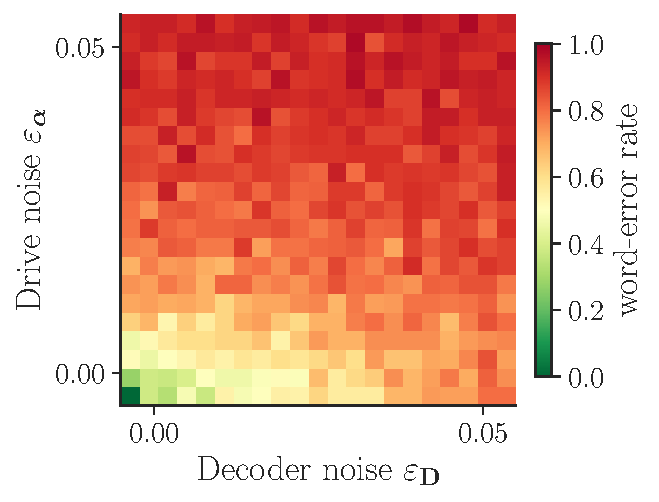
\includegraphics[width=0.6\textwidth]{figures/combined_noise.pdf}
\caption{Combined drive- and decoder-noise robustness scan for the $K=N=3$ symmetric system with the period-11 reference word ($|\mu_2/\mu_1|=0.015$). Multiplicative noise $\varepsilon_{\boldsymbol{\alpha}}$ rescales each drive by $1+\varepsilon_{\boldsymbol{\alpha}}\eta$ ($\eta\sim\mathcal{N}(0,1)$) and likewise per-component for each decoder (then renormalized to unit length). Each cell reports the word-error rate over 25 trials. The dashed iso-contour at 50\% error sits in the $\varepsilon\lesssim 0.02$ region; biologically plausible noise levels ($\varepsilon\sim 0.05$--$0.10$) lie in the saturated upper-right region where the exact firing word is essentially never recovered.}
\label{fig:combined-noise}
\end{figure}


\section{Rate-versus-sequence robustness discussion (main text \S 5)}\label{app:rate-vs-seq}

\paragraph{Robustness of rate versus sequence codes.}
The inverse problem solved here treats the exact firing word $\sigma$ as the quantity to realize, but the analysis of Section~\ref{sec:bifurcation} suggests a more robust encoding may be available. The firing-ratio map $\rho(\boldsymbol{\alpha})$ is a complete devil's staircase on rational rotation numbers \citep[Arnold tongues for analytic circle maps;][]{arnold1961small,herman1979conjugaison}, restated for our family as Theorem~\ref{thm:staircase}, and \emph{within each plateau} the rotation number is exactly invariant under small input perturbations. For $K=2$, Sturmian uniqueness (Remark~\ref{rem:sturmian}) then forces the exact word $\sigma$ to be locked alongside $\rho$, so the rate code and the sequence code coincide on each plateau. For $K\geq 3$ this coincidence breaks: the partition geometry permits several admissible words with the same firing-ratio vector $(\rho_1,\ldots,\rho_K)$, so the word can shift between admissible variants under a perturbation that leaves the rotation number invariant. The robust storage substrate is therefore not the exact spike-by-spike sequence but the \emph{rotation number}, equivalently, the rational plateau the system occupies on the staircase. Under time-varying input the system traces a piecewise-constant trajectory through $\rho$-space, hopping between plateaus, and the temporal code that survives input perturbation is this sequence of plateau visits rather than the underlying spike sequence on each. The inverse problem we solve here treats the exact spike sequence as the quantity to realize and is therefore fragile to input perturbations; the staircase plateaus themselves preserve only the rotation number and are robust at this coarser level. Distinguishing the two experimentally, are sequence-encoding cortical circuits robust at the level of exact spike order or only at the level of population firing ratios?, is a falsifiable prediction the framework offers.


\section{Analytical robustness bound via eigenvector perturbation (main text \S 5)}\label{app:analyt-bound}

\paragraph{Analytical robustness bound.} The tolerance to parameter perturbation can be predicted from eigenvector perturbation theory (the non-symmetric analogue of the Davis--Kahan theorem \citep{davis1970rotation,stewart1990matrix}). For a simple eigenvalue $\mu_1$ of $\vv{M}_\sigma$ with right eigenvector $\vv{u}_1$ and left eigenvector $\vv{w}_1$, a perturbation $\delta\vv{M}$ shifts the eigenvector by
\begin{equation}\label{eq:eigpert}
    \delta\vv{u}_1 = \sum_{k=2}^{N}\frac{\vv{w}_k^\top(\delta\vv{M})\vv{u}_1}{\mu_1-\mu_k}\,\vv{u}_k.
\end{equation}
The denominator $\mu_1-\mu_k$ is the eigenvalue gap: larger gap means smaller perturbation. After dehomogenization, the orbit shift is $\delta\xxi^*=(1/u_N)[\delta\vv{u}_{1:N-1}-\xxi^*\,\delta u_N]$. The orbit survives perturbation $\delta\boldsymbol{\alpha}$ iff $\|\delta\xxi^*\|$ is small enough that the margin remains positive. This yields the tolerance bound
\begin{equation}\label{eq:tolerance}
    \text{tolerance}\;\approx\;\frac{m}{\|\nabla_{\boldsymbol{\alpha}}m\|}\;\propto\;\frac{m\cdot|\mu_1-\mu_2|}{\|\partial\vv{M}_\sigma/\partial\boldsymbol{\alpha}\|\cdot\kappa(\vv{S})},
\end{equation}
where $\kappa(\vv{S})$ is the condition number of the eigenvector matrix. For the RBYGYB orbit, this predicts per-drive tolerances of $0.6$--$19\%$ (tightest on $\alpha_3,\alpha_4$), matching the actual values to within a factor of~2 (Appendix~\ref{app:numerics}). Robustness is thus jointly controlled by the admissibility margin $m$ (geometric) and the eigenvalue gap $|\mu_1-\mu_2|$ (dynamical).

\section{Glossary}\label{sec:glossary}

Throughout, each ``spike'' is an instantaneous Dirac-$\delta$ event in continuous time, and the discrete index $n$ in expressions like $\xxi_n$, $b_n$, or ``step $n$'' counts \emph{spike events} (not equispaced time steps): one $n$-step corresponds to one spike-and-decay segment of continuous time.

\begin{table}[h]
\centering
\small
\renewcommand{\arraystretch}{1.05}
\begin{tabular}{ll}
\hline
Symbol & Meaning \\
\hline
$K,\ N$ & number of neurons; ambient (input) dimension \\
$\DD_i\in\RR^N$ & unit-norm decoder of neuron $i$ \\
$\alpha_i>0$ & suprathreshold drive of neuron $i$ (after change of variables) \\
$\psi_{ij}$ & angle between decoders, $\cos\psi_{ij}=\DD_i^\top\DD_j$ \\
$\yy\in\RR^N$ & readout / population response \\
$\Bsp_i=\{\yy:\DD_i^\top\yy=\alpha_i\}$ & spike bound for neuron $i$ \\
$\vv{U}_i\in\RR^{N\times(N-1)}$ & orthonormal tangent frame of $\Bsp_i$ \\
$\xxi\in\RR^{N-1}$ & tangent coordinate on a bound \\
$\yy^+=\yy+\DD_i$ & post-spike readout after neuron $i$ fires \\
$c_j(\xxi)=\alpha_j/(\DD_j^\top\yy^+)$ & decay factor; next firer maximises $c_j$ \\
$\vv{M}_{j\leftarrow i}\in\RR^{N\times N}$ & per-step transition matrix in homogeneous coordinates \\
$\sigma=(b_0,\ldots,b_{L-1})$ & firing word (sequence of fired neurons) of length $L$ \\
$\vv{M}_\sigma$ & return matrix, $\vv{M}_{b_0\leftarrow b_{L-1}}\cdots\vv{M}_{b_2\leftarrow b_1}\vv{M}_{b_1\leftarrow b_0}$ (right-to-left composition) \\
$\xxi^*$ & dehomogenized dominant eigenvector of $\vv{M}_\sigma$; orbit position on $\Bsp_{b_0}$ \\
$\mu_1,\ldots,\mu_N$ & eigenvalues of $\vv{M}_\sigma$, ordered by decreasing modulus \\
$|\mu_k/\mu_1|$ for $k\geq 2$ & Lyapunov multipliers; orbit stable iff all $<1$ \\
$\rho$ & rotation number / firing ratio of neuron 3 \\
$m(\alpha_2)$ & admissibility margin (continuous score, $>0$ iff $\sigma$ realised) \\
\hline
\end{tabular}
\caption{Notation used throughout. Lower-case bold for vectors, upper-case bold for matrices; calligraphic letters for sets and bounds.}
\label{tab:notation}
\end{table}

\section{Numerical experiment details}\label{app:numerics}
%======================================================================

All experiments were implemented in Python~3.12 using NumPy and SciPy. This appendix specifies every parameter choice needed to reproduce the results.

\subsection{Forward simulation}\label{app:forward-sim}

Every forward simulation uses the same core routine. Starting from an initial tangent coordinate $\xxi_0$ and bound index $b_0$, each step applies the transition map~\eqref{eq:transition-map} by:
\begin{enumerate}[nosep]
    \item Computing the post-spike readout $\yy^+=(\alpha_{b_k}+1)\DD_{b_k}+\vv{U}_{b_k}\xxi_k$.
    \item For each active neuron~$j$ ($\alpha_j>0$), computing the decay factor $c_j=\alpha_j/(\DD_j^\top\yy^+)$.
    \item Selecting $j^*=\arg\max_j c_j$ (subject to $0<c_j\leq 1$).
    \item Landing: $\xxi_{k+1}=\vv{U}_{j^*}^\top(c_{j^*}\yy^+)$.
\end{enumerate}
No ODE solver is needed; the dynamics are exact in discrete time.

\subsection{Figure~\ref{fig:overview-supp}: SCN overview ($N{=}K{=}2$)}\label{app:fig-overview}

Decoder angles $	heta_1=0.25$\,rad, $	heta_2=	heta_1+0.4\pi$\,rad, giving $\psi=0.4\pi$, $\cos\psi\approx 0.309$.

\textbf{Panels (a,b):} Drives $\alpha_1=1.0$, $\alpha_2=0.49$. Orbit found by simulating 5\,000 transient steps from $\xi_0=1.0$ on bound~1, then recording 7~steps. The period-7 word $\sigma=(1,1,2,1,1,1,2)$ and orbit position $\xi^*\approx 0.717$ are verified against the dominant eigenvector of the $2\times 2$ return map $\vv{M}_\sigma$.

\textbf{Panel (c):} First-return map $F_{\!\Bsp_1}:\Bsp_1\to\Bsp_1$, mapping the tangent coordinate $\xi_n$ on bound~1 to the next visit $\xi_{n'}$ on bound~1. Two branches separated by the partition point $\xi_{\mathrm{part}}\approx 0.381$: for $\xi<\xi_{\mathrm{part}}$, the decay factor $c_2>c_1$ so neuron~2 fires next (cross-transition); for $\xi\geq\xi_{\mathrm{part}}$, $c_1>c_2$ so neuron~1 self-fires. Each branch is a M\"obius transformation $\xi\mapsto(a\xi+b)/(c\xi+d)$. The period-7 orbit visits $\Bsp_1$ five times per cycle, so the cobweb converges to a 5-cycle of the first-return map.

\textbf{Panel (d):} Devil's staircase computed by scanning $\alpha_2\in[0.01,\,1.0]$ at $600$ uniformly spaced values. At each value: $5{,}000$ transient steps from four different initial conditions ($\xi_0\in\{0.05,\,0.5,\,1.0,\,1.5\}$), selecting the mixed orbit when found.  Period detection from $300$ recorded steps (requiring $\min(3L,30)$ consecutive matches).  Purple dots mark every distinct plateau with $\rho>0$.

\subsection{Figure~\ref{fig:cobweb_gallery}: Cobweb gallery across the staircase}\label{app:cobweb-gallery}

The cobweb diagram provides a direct visualization of the 
piecewise projective return map as a classical dynamical system on 
the line.  For $K{=}2$, $N{=}2$, the full dynamics reduce to a 
first-return map $F_{\!\Bsp_1}:\Bsp_1\to\Bsp_1$ with two branches, each a
M\"obius transformation:
\begin{itemize}[nosep]
\item \emph{Cross branch} ($\xi<\xi_{\mathrm{part}}$): $c_2>c_1$, 
so neuron~2 fires next.  The readout visits $\Bsp_2$ before returning 
to $\Bsp_1$, giving $F(\xi)=\alpha_1 \cdot
[(\alpha_2+1)\vv{w}_{01}+\vv{R}_{01}\,\alpha_2\,\{(\alpha_1+1)\vv{w}_{10}+\vv{R}_{10}\xi\}/
\{(\alpha_1+1)\cos\psi_{21}+\vv{v}_{10}\xi\}] / [\cdots]$ (composition of two
transition maps).
\item \emph{Self branch} ($\xi\geq\xi_{\mathrm{part}}$): $c_1>c_2$, 
so neuron~1 self-fires.  The map is simply 
$F(\xi)=\alpha_1\xi/(\alpha_1+1)$, a uniform contraction toward the 
foot $\xi=0$.
\end{itemize}
The partition point $\xi_{\mathrm{part}}$ is the unique $\xi$ where 
$c_1=c_2$, i.e.\ $\alpha_1/(\alpha_1+1)=\alpha_2/\{(\alpha_1+1)\cos\psi_{21}+\vv{v}_{10}\xi\}$.  
As $\alpha_2$ increases, $\xi_{\mathrm{part}}$ decreases (the cross 
region grows), and the orbit visits $\Bsp_2$ more frequently, 
increasing~$\rho$.

Figure~\ref{fig:cobweb_gallery} shows the first-return map and cobweb 
at eight values of $\alpha_2$, one per distinct mode-locked plateau.  
The key observations are:
\begin{enumerate}[nosep]
\item At $\alpha_2=0.20$ (below threshold), only the self branch 
exists: $F(\xi)=0.5\xi$, converging to the fixed point $\xi^*=0$ 
(period-1 self-trap, $\rho=0$).
\item At $\alpha_2=0.335$ ($\rho=1/6$), the cross branch has appeared 
and the cobweb traces a 5-cycle on $\Bsp_1$ (five of six orbit steps 
land on~$\Bsp_1$).
\item At $\alpha_2=0.60$ ($\rho=1/3$, the widest mixed plateau at 
width~$0.10$), the cobweb traces a 2-cycle: each visit to $\Bsp_1$ 
alternates between a self-transition and a cross-transition.
\item At $\alpha_2=0.80$ ($\rho=3/7$), the cobweb traces a 4-cycle 
with three cross-transitions per period.
\end{enumerate}
In every case, the cobweb converges to a periodic cycle (never a fixed 
point, except at $\rho=0$), confirming that the first-return map is a
degree-$1$ piecewise-M\"obius map with a unique stable periodic orbit at each
rational rotation number.

\begin{figure}[t]
\centering
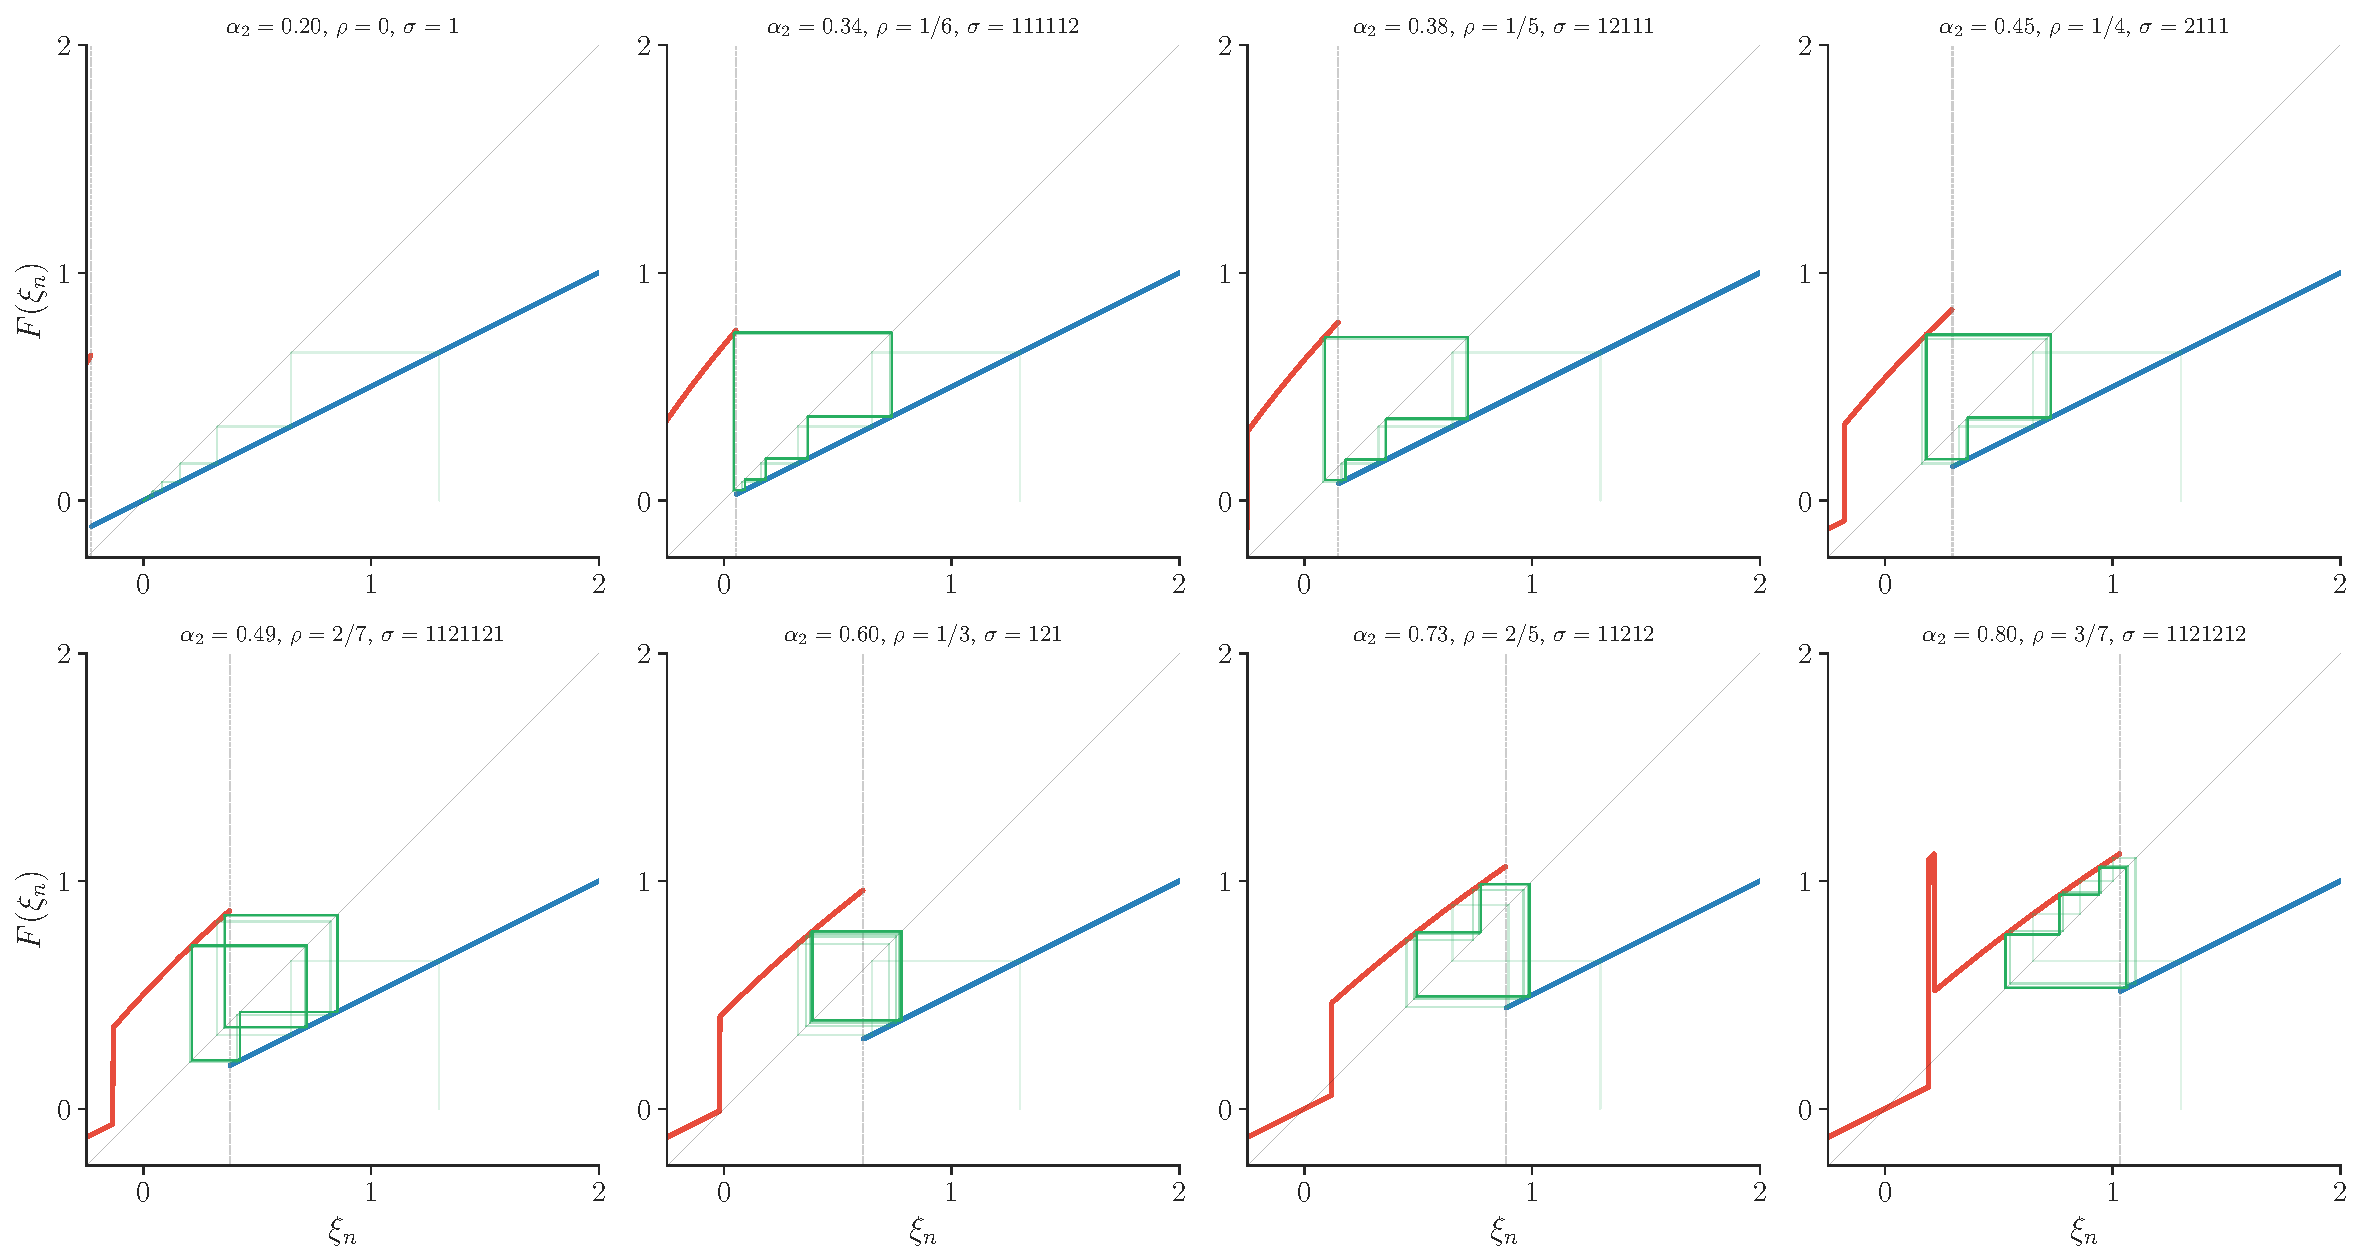
\includegraphics[width=\textwidth]{figures/cobweb_gallery.pdf}
\caption{Cobweb diagrams of the first-return map $F_{\!\Bsp_1}:\Bsp_1\to\Bsp_1$ at eight values of $\alpha_2$, one per distinct mode-locked plateau of the devil's staircase.  Red: cross-transition branch ($\xi<\xi_{\mathrm{part}}$); blue: self-transition branch ($\xi\geq\xi_{\mathrm{part}}$); dashed: partition point.  Green cobwebs (from $\xi_0=1.3$) converge to the unique stable cycle, whose period on~$\Bsp_2$ equals the number of~1's in the firing word~$\sigma$.}
\label{fig:cobweb_gallery}
\end{figure}

\subsection{Staircase orbit examples ($K{=}N{=}2$)}\label{app:staircase-examples}

Figures~\ref{fig:staircase1}--\ref{fig:staircase8} show all 48 
distinct mode-locked orbits found in the devil's staircase scan of 
Figure~\ref{fig:overview-supp}d, organized into eight pages of six panels 
each.  Each panel displays the orbit in $\RR^2$ at a single 
$\alpha_2$ value (with $\alpha_1=1.0$, $\psi=0.4\pi$ throughout):
\begin{itemize}[nosep]
\item \emph{Top row:} Eigenvector-predicted orbit positions (colored 
dots from the dominant eigenvector of $\vv{M}_\sigma$), with spike 
(colored) and decay (gray dashed) connections.
\item \emph{Bottom row:} Simulation from a random initial condition, 
converging to the same positions.
\end{itemize}
In every case, theory and simulation match to machine precision.  
The orbits span firing ratios from $\rho_{\text{spike}}=1/8$ (period~8, one
neuron-1 firing per cycle) to $\rho_{\text{spike}}=4/9$ (period~9, nearly equal
firing rates).  The firing words are all Sturmian 
(Remark~3): for any two subwords of the same length, the 
neuron-1 count differs by at most~1.

\begin{figure}[p]
\centering
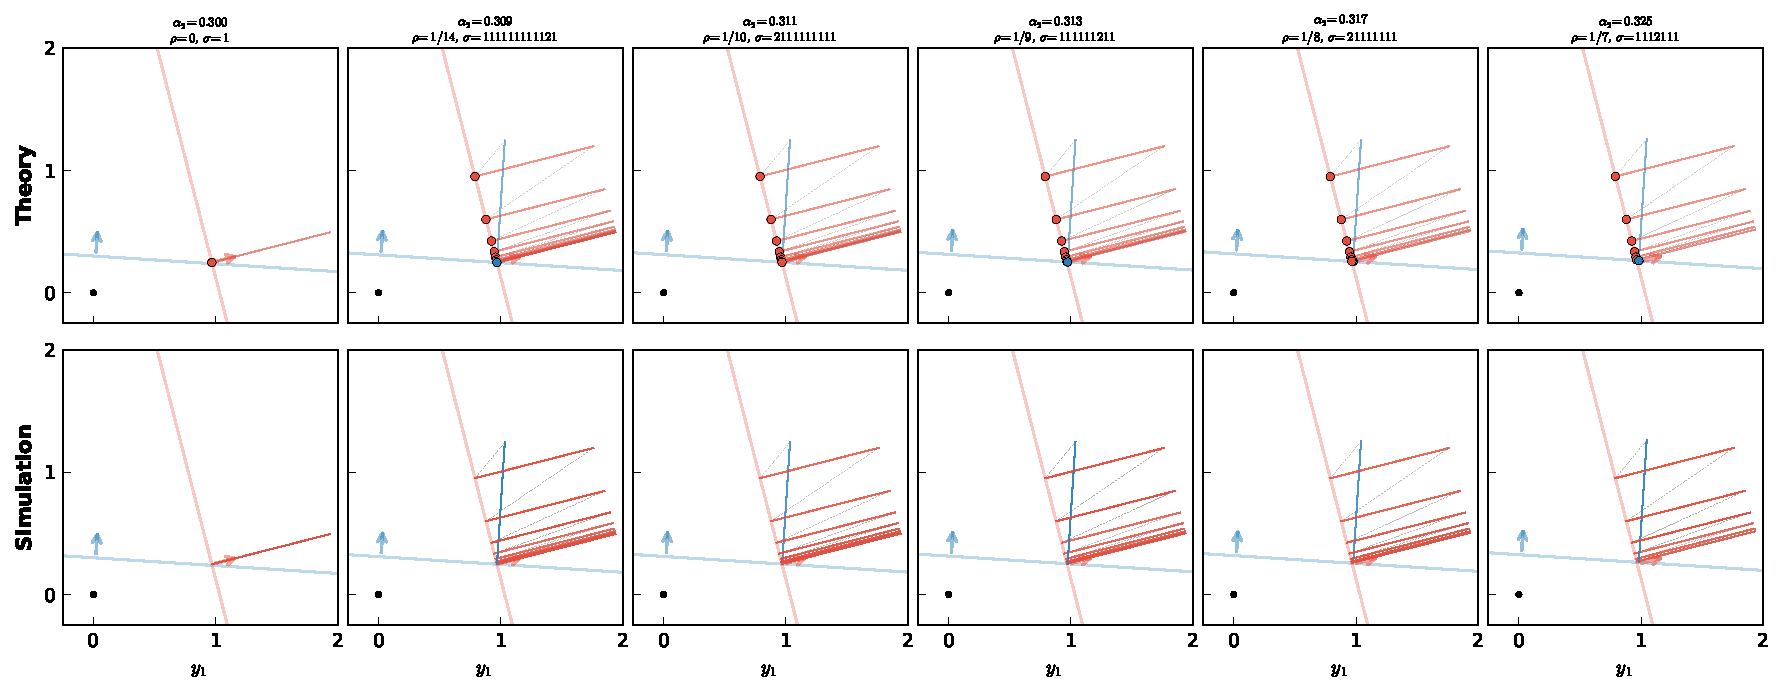
\includegraphics[width=\textwidth]{figures/staircase_examples_1.pdf}
\caption{Staircase orbit examples, page 1 of 8.}
\label{fig:staircase1}
\end{figure}

\begin{figure}[p]
\centering
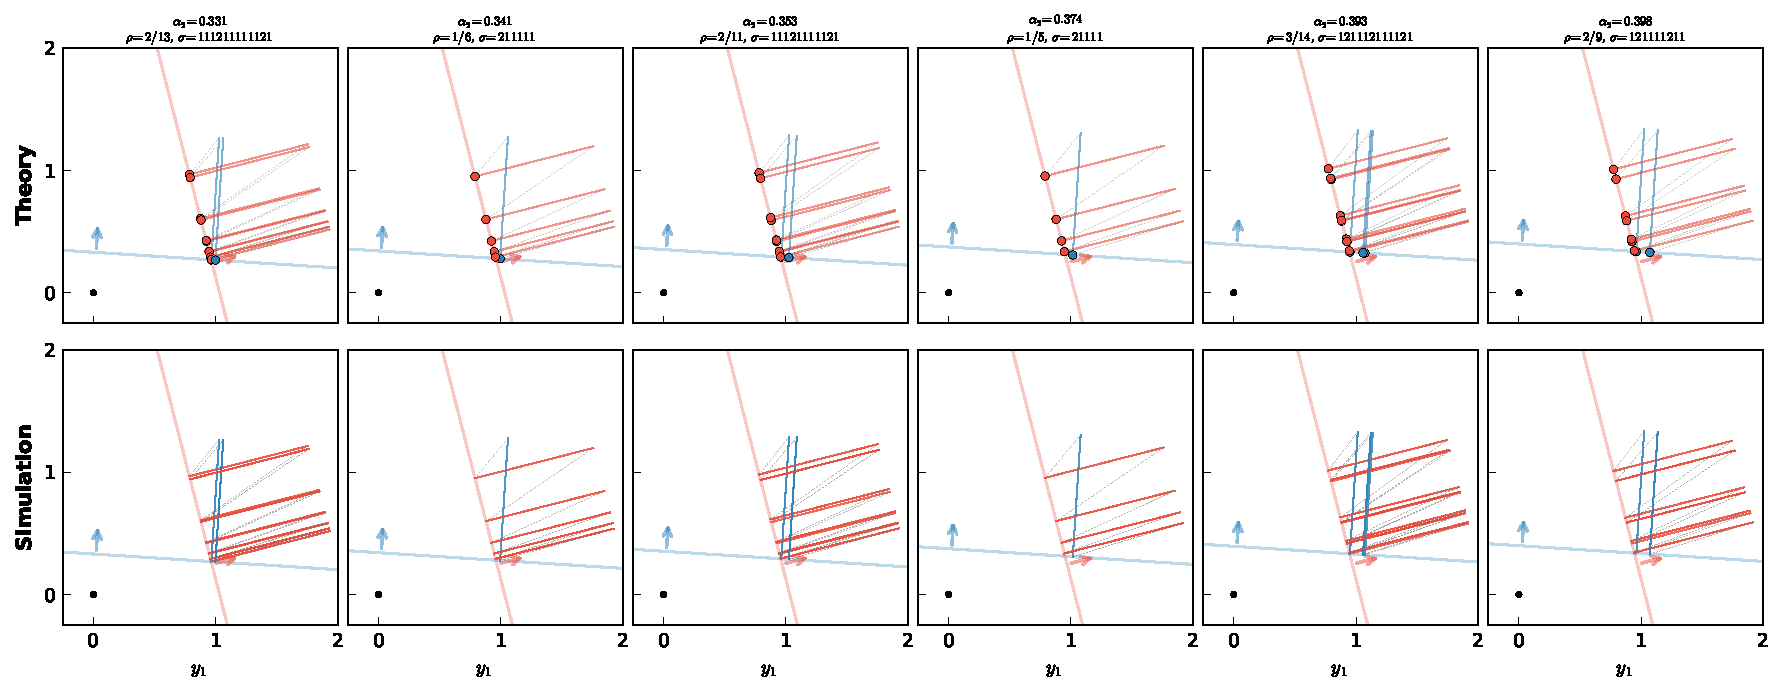
\includegraphics[width=\textwidth]{figures/staircase_examples_2.pdf}
\caption{Staircase orbit examples, page 2 of 8.}
\label{fig:staircase2}
\end{figure}

\begin{figure}[p]
\centering
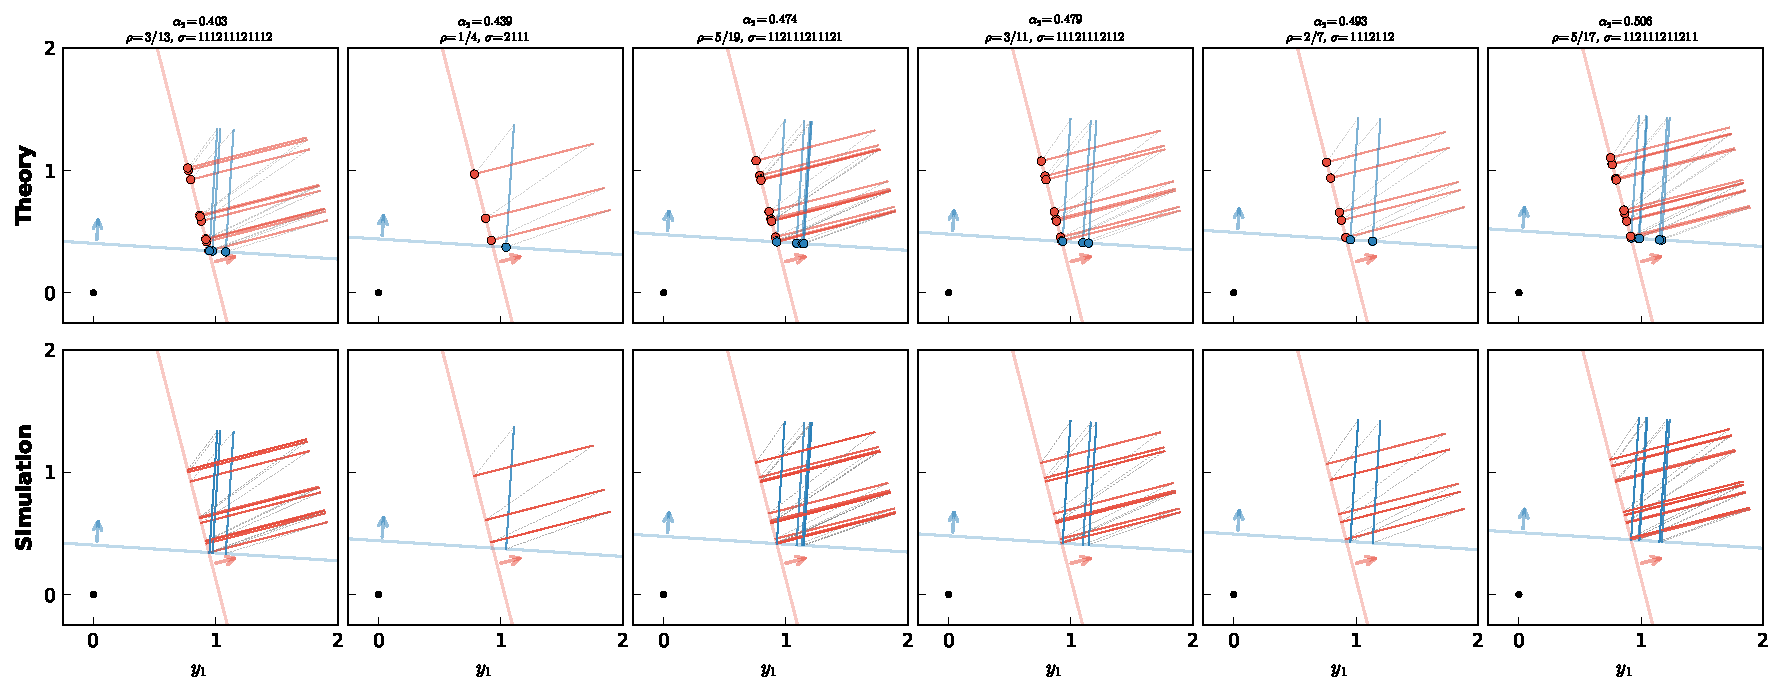
\includegraphics[width=\textwidth]{figures/staircase_examples_3.pdf}
\caption{Staircase orbit examples, page 3 of 8.}
\label{fig:staircase3}
\end{figure}

\begin{figure}[p]
\centering
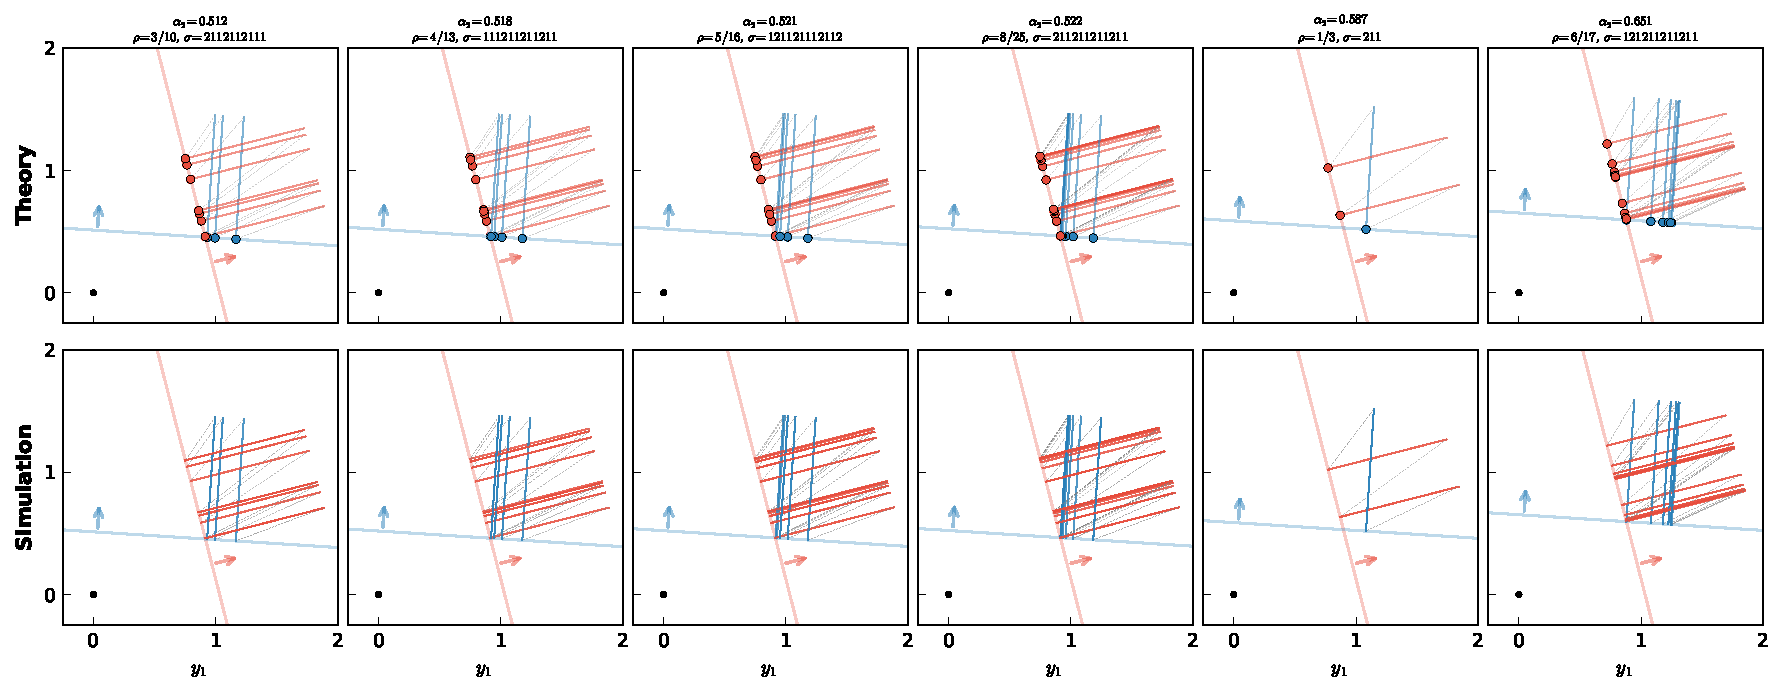
\includegraphics[width=\textwidth]{figures/staircase_examples_4.pdf}
\caption{Staircase orbit examples, page 4 of 8.}
\label{fig:staircase4}
\end{figure}

\begin{figure}[p]
\centering
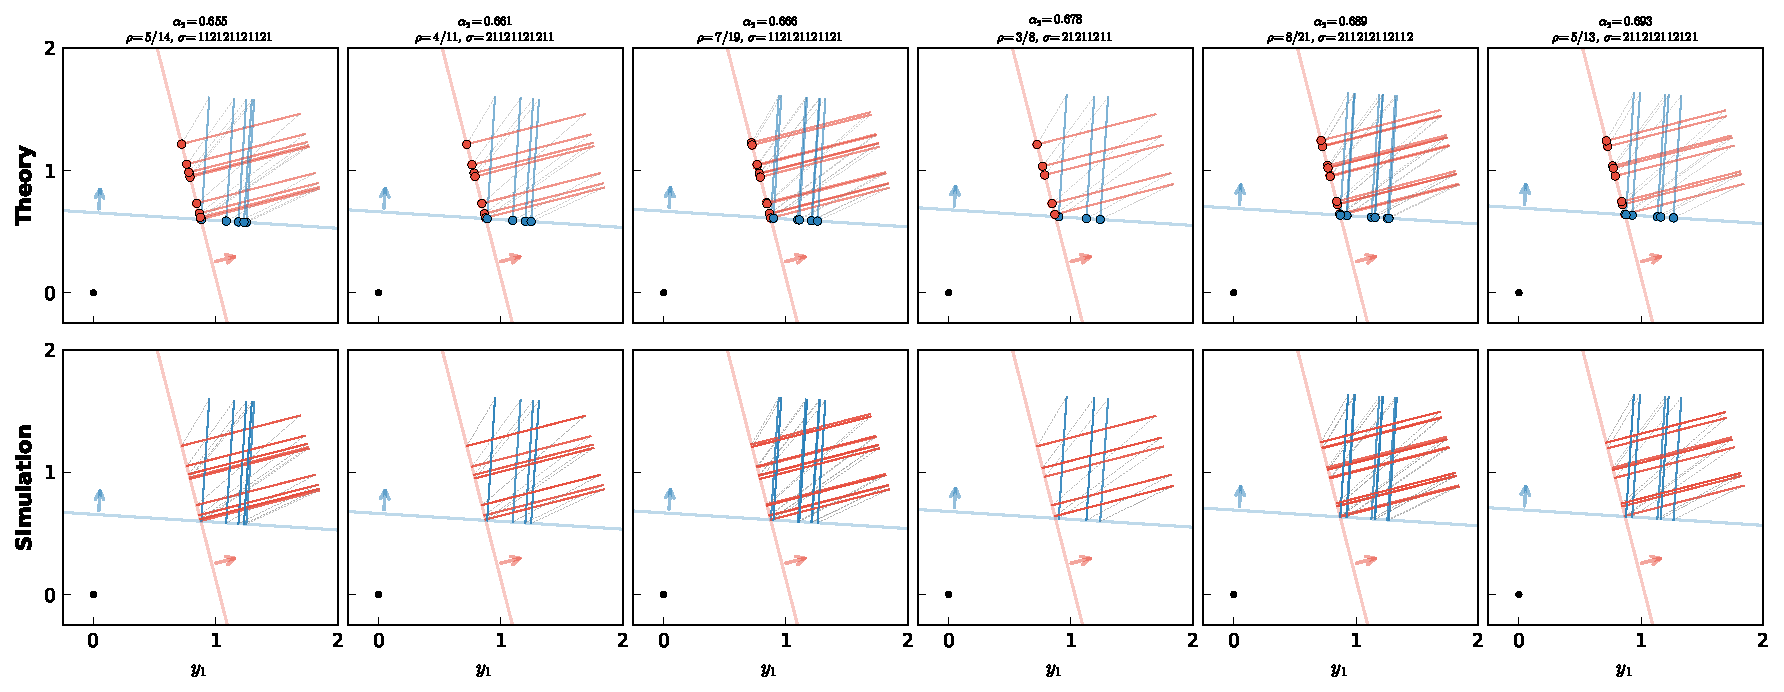
\includegraphics[width=\textwidth]{figures/staircase_examples_5.pdf}
\caption{Staircase orbit examples, page 5 of 8.}
\label{fig:staircase5}
\end{figure}

\begin{figure}[p]
\centering
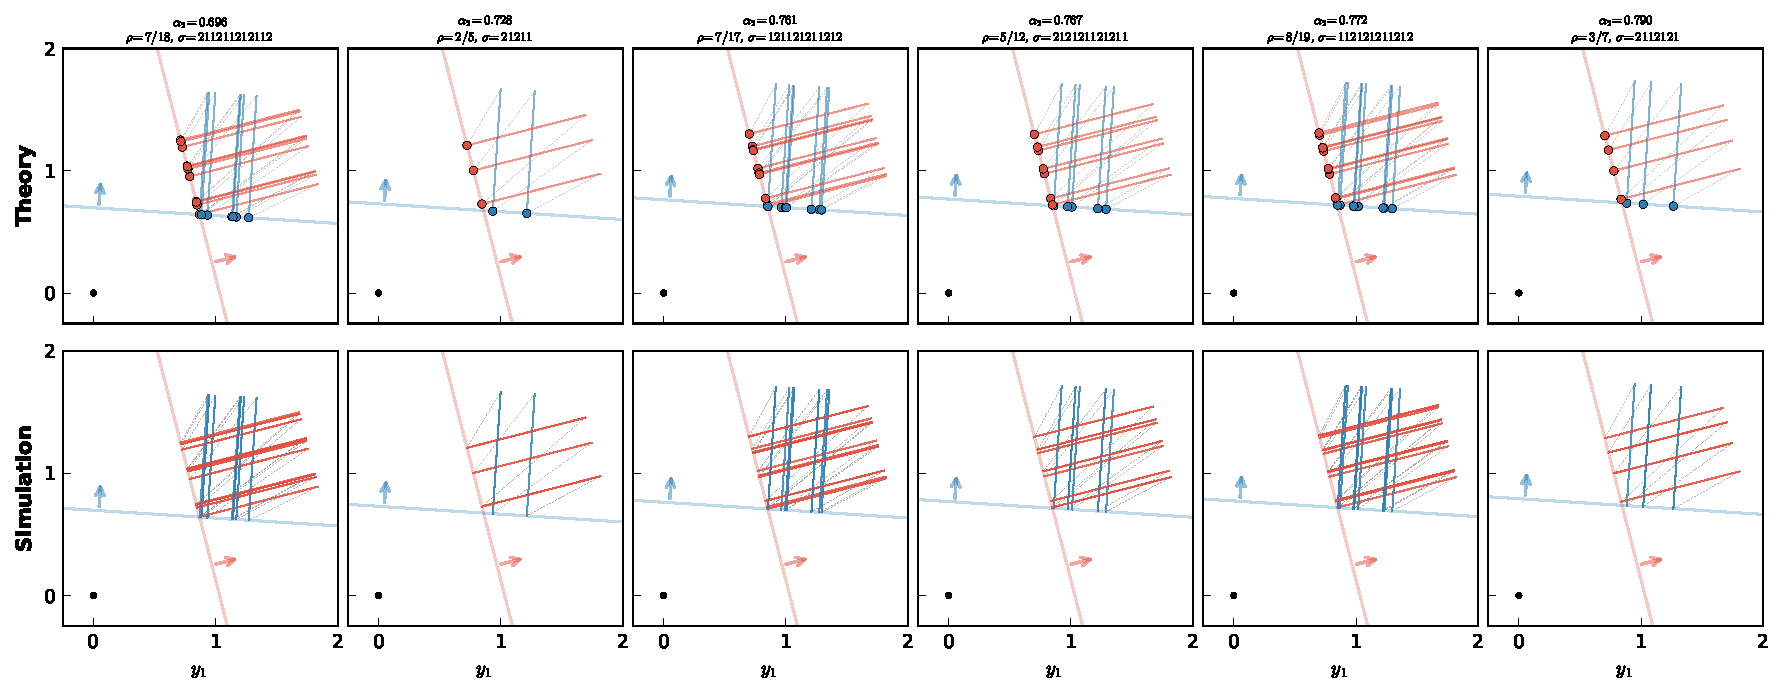
\includegraphics[width=\textwidth]{figures/staircase_examples_6.pdf}
\caption{Staircase orbit examples, page 6 of 8.}
\label{fig:staircase6}
\end{figure}

\begin{figure}[p]
\centering
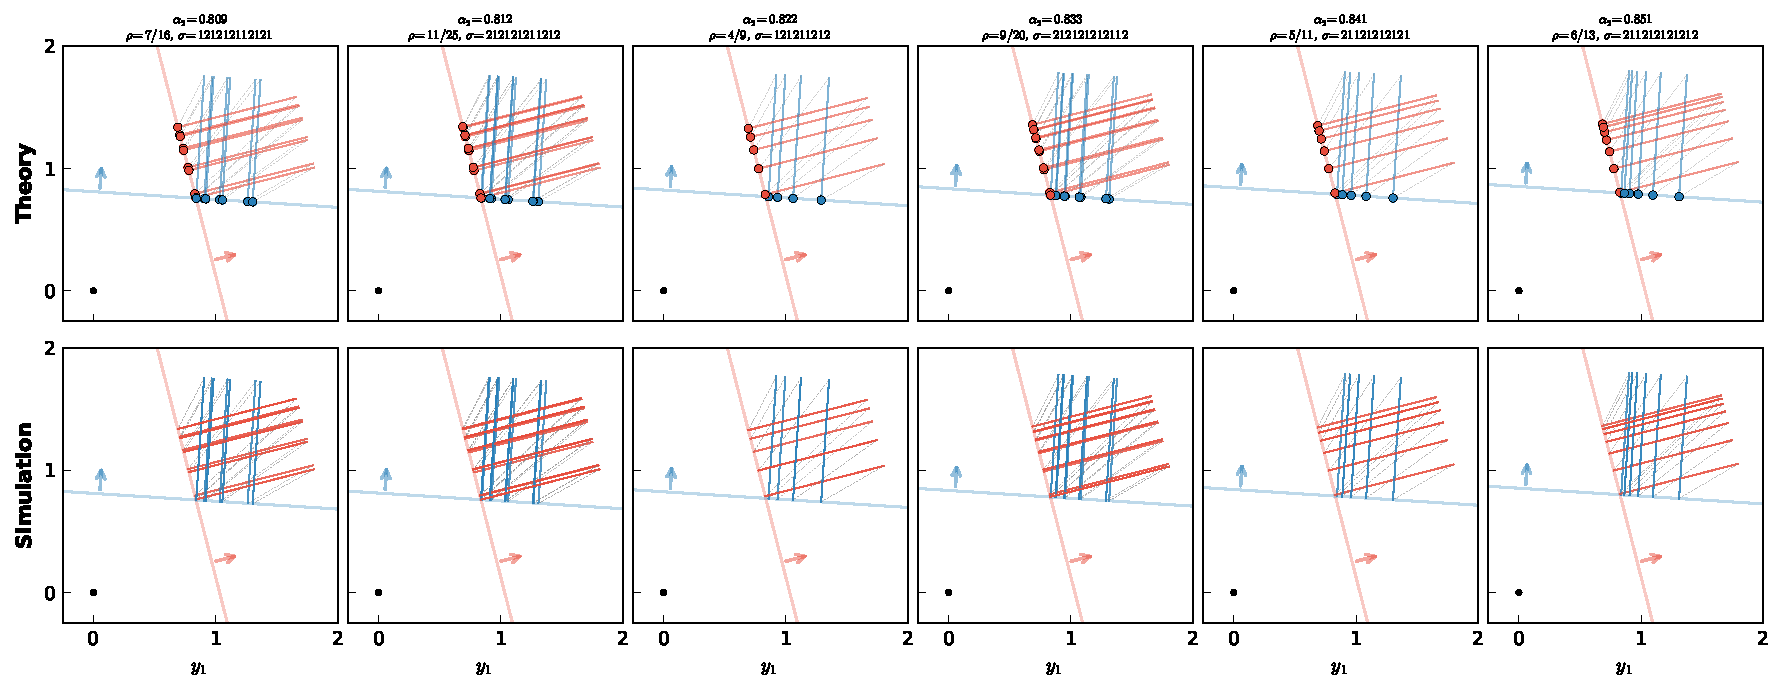
\includegraphics[width=\textwidth]{figures/staircase_examples_7.pdf}
\caption{Staircase orbit examples, page 7 of 8.}
\label{fig:staircase7}
\end{figure}

\begin{figure}[p]
\centering
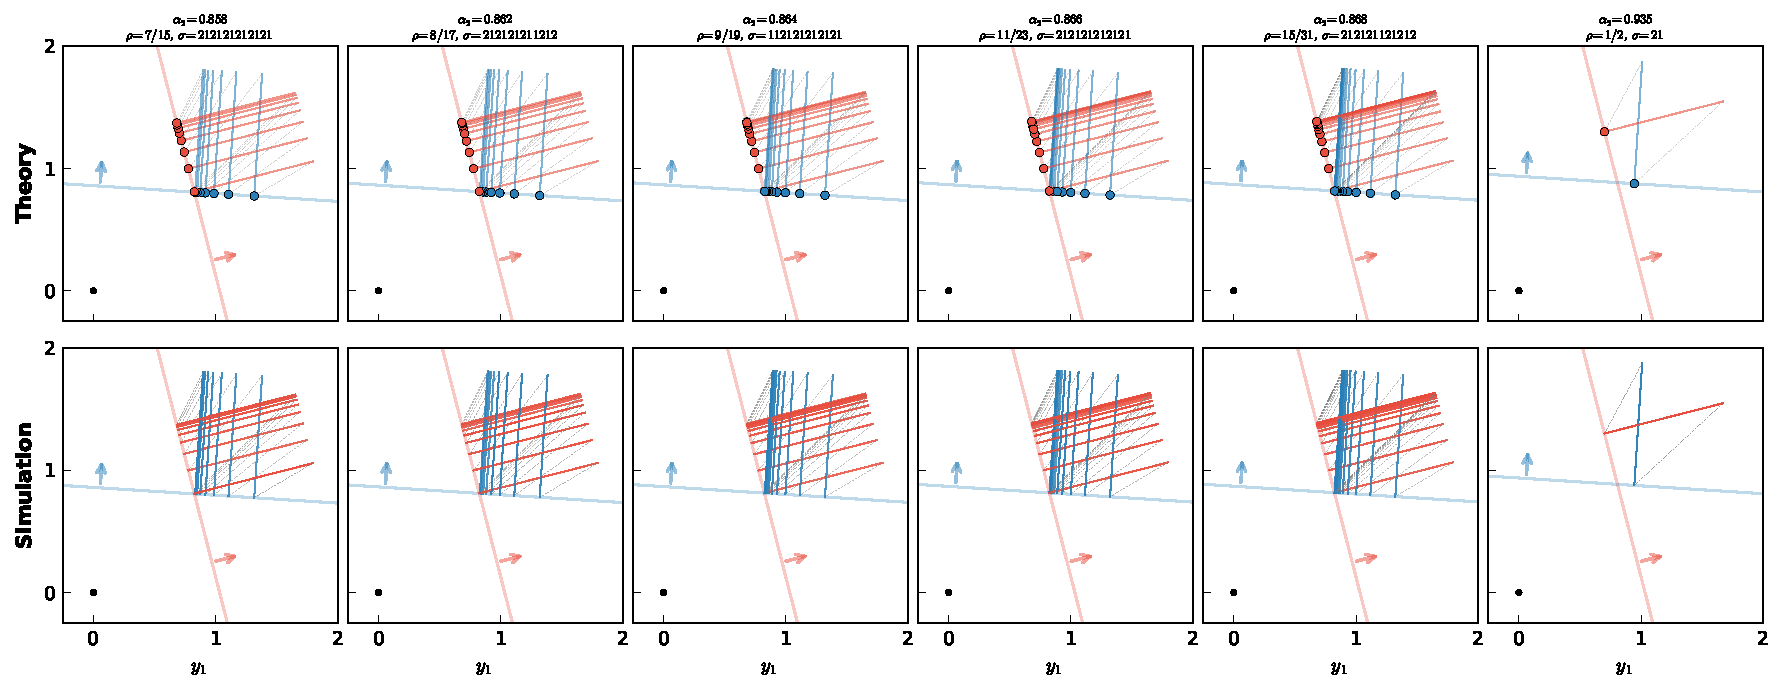
\includegraphics[width=\textwidth]{figures/staircase_examples_8.pdf}
\caption{Staircase orbit examples, page 8 of 8.}
\label{fig:staircase8}
\end{figure}

\subsection{Figure~\ref{fig:chaos}: Order-chaos transition ($K{=}4$, $N{=}3$)}\label{app:fig-chaos}

\textbf{Chaotic system:} Decoders (each unit-normalized) and drives:
\begin{align*}
\DD_1 &\approx (0.566,\,-0.791,\,-0.233), & \DD_2 &\approx (0.748,\,-0.260,\,0.611), \\
\DD_3 &\approx (-0.296,\,-0.526,\,-0.798), & \DD_4 &\approx (0.694,\,-0.601,\,0.395), \\
\boldsymbol{\alpha} &\approx (0.966,\,0.342,\,0.487,\,0.653). & &
\end{align*}
Pairwise cosines include the minimum $\cos\psi_{23}\approx -0.57$ (and $\cos\psi_{34}\approx -0.20$).

\textbf{Panel (a): phase diagram.} 800~random $(\vv{D},\boldsymbol{\alpha})$ configurations with $K=4$, $N=3$. Decoders: rows of a $4\times 3$ standard normal matrix, unit-normalized. Drives: i.i.d.\ $\text{Exp}(0.8)$. Random seed~42. Per sample: 1\,500~transient steps + 3\,000~recording steps. Classification: $\lambda_{\max}>0$ = chaotic ($5$ cases out of $800$, including one weakly chaotic case with $\lambda_{\max}\approx 0.004$), all with $\min_{i<j}\cos\psi_{ij}<-0.5$. The accent-blue open square marks the specific chaotic configuration used in panels~(b) and~(c) (constructed to prove chaos; not one of the 800 random samples).

\textbf{Panel (b): sensitivity to initial conditions.} After a $10\,000$-step transient off a random seed on bound~$\Bsp_1$, we pre-record $400\cdot 12+1=4801$ consecutive steps of the converged chaotic orbit. Each of $400$ perturbation pairs is anchored at a different point along that trajectory (spacing $12$ steps between successive anchors), perturbed by $\varepsilon=10^{-12}$ in a random unit tangent direction (seed~0). Each pair is tracked for $150$~steps; median and inter-quartile range of the ambient-space distance $\|\yy^{\mathrm{ref}}_t-\yy^{\mathrm{pert}}_t\|$ are plotted on a log scale. The dashed reference line is $\varepsilon\cdot e^{\lambda_{\max}t}$ with $\lambda_{\max}$ set to the QR-measured value from the Lyapunov calculation below.

\textbf{Lyapunov spectrum.} We report two consistent measurements. \emph{(1)~Twin-trajectory:} after $5\,000$~transient steps, initialize a twin at $\varepsilon=10^{-9}$; at each step record $\ln(\|\delta\xxi\|/\varepsilon)$ and renormalize. Converges to $\lambda_{\max}=0.282\pm 0.002$ over $20\,000$~steps. \emph{(2)~QR accumulation of a $2\times 2$ per-step Jacobian:} the accompanying code (\texttt{code/fig\_chaos.py}) uses a central finite difference with step size $10^{-6}$, one-sided on the branch flip fallback; a symbolic analytic Jacobian is derivable in closed form from the transition map~\eqref{eq:transition-map} as $\vv{J}(\xxi)=(1/\delta)(\alpha_j\vv{R}_{ji}-\xxi'\vv{v}_{ji}^\top)$ (see the proof of Theorem~\ref{thm:cone}(b)). Accumulation is by QR every step over $50$~segments of $1000$~steps after a $10\,000$-step transient. Result: $\lambda_1=0.288$, $\lambda_2=-0.388$ nats/step (agreement with the paper-cited $\lambda_1=0.285\pm 0.010$, $\lambda_2=-0.389\pm 0.008$ from the analytic-Jacobian run), with all $50$ segments giving $\lambda_1>0.26$.

\textbf{Panel (c): strange attractor.} $50\,000$~iterates from the converged state; the ${\sim}20\,000$ visits to $\Bsp_3$ (the most frequently visited bound) are plotted in the tangent chart $(\xi_1,\xi_2)$.

\subsection{Figure~\ref{fig:simon}: Sequence working memory ($K{=}4$, $N{=}3$)}\label{app:fig-simon}

\textbf{Decoders:} Four unit vectors arranged symmetrically around the $(1,1,1)/\sqrt{3}$ axis:
$\DD_i = (1,1,1)/\sqrt{3} + 0.6[\cos(i\pi/2)\,\vv{u}_1+\sin(i\pi/2)\,\vv{u}_2]$,
where $\vv{u}_1=(1,-1,0)/\sqrt{2}$, $\vv{u}_2=\vv{u}_1\times(1,1,1)/\sqrt{3}$, for $i=0,1,2,3$, each unit-normalized. All pairwise cosines are positive ($\cos\psi\approx 0.47$).

\textbf{Panel (b):} Drives $\boldsymbol{\alpha}=(2.02,\,2.05,\,2.43,\,2.35)$, producing the period-6 word $\sigma=\text{RBYGYB}=(1,3,4,2,4,3)$. Orbit positions from the dominant eigenvector of the $3\times 3$ return map $\vv{M}_\sigma$. Transient trajectory: 48~steps from $\xxi_0=(0,0)$ on bound~1.

\textbf{Panel (c), noise robustness:} 30~log-spaced noise levels $\eta_{\text{std}}\in[10^{-3.5},\,10^{-0.3}]$. At each level, 30~independent trials (seeds 0--29). Each trial: 200~noiseless transient steps to converge, then 600~noisy steps. Noise model: S1-type additive Gaussian $\boldsymbol{\eta}\sim\mathcal{N}(\vv{0},\eta_{\text{std}}^2\vv{I}_3)$ added to the post-spike readout $\yy^+$ before decay. Word error rate = (number of steps where $b_k\neq\sigma_{k\bmod L}$)/(total steps). Admissibility margin for this orbit: $m\approx 0.005$.

\subsection{Figure~\ref{fig:3d}: Three-neuron example ($K{=}N{=}3$)}\label{app:fig-3d}

Three decoders in $\RR^3$ arranged symmetrically about the axis
$[1,1,1]^\top/\sqrt{3}$ with pairwise cosines
$\cos\psi_{ij}=0.507$ for all pairs.  Drives
$\boldsymbol{\alpha}=(1.0,\,0.9,\,0.7)$.

\textbf{Panel~(a).}
Geometry rendered at elevation $70^\circ$, azimuth $180^\circ$.
Each bound $\Bsp_i$ is shown as a filled rectangle in the plane
$\DD_i^\top\yy=\alpha_i$, sized to cover the orbit points and
the foot $\alpha_i\DD_i$.  The $11$ colored dots are the
eigenvector-predicted orbit positions; spike (colored) and decay
(gray dashed) segments connect consecutive points.

\textbf{Panel~(b).}
Converged firing pattern over two full periods ($22$~steps), started
from the eigenvector $\xxi^*$.  Each trace shows
$\DD_j^\top\yy$ for $j=0,1,2$; dots mark which neuron fires.
Dashed horizontal lines indicate the thresholds $\alpha_j$.

\textbf{Panel~(c).}
Convergence to the limit cycle from $500$ random initial conditions
($\xxi_0\sim\mathcal{N}(\mathbf{0},\,1.5^2\vv{I})$, $b_0$ uniform on
$\{0,1,2\}$).  At each step~$n$, the distance to the limit cycle is
$\min_{k:\,b_k=b_{\text{sim}}} \|\xxi_{\text{sim}}-\xxi_k^*\|$,
i.e.\ the minimum over all theory points on the same bound
(accounting for phase).  Of the $500$ trials, $448$ ($90\%$) converge
to the period-11 orbit; the remaining $52$ ($10\%$) self-trap on
$\Bsp_3$.  Statistics are computed over the converging subset only.
The dashed line shows the theoretical envelope
$C\,|\mu_2/\mu_1|^{n/L}$ with $|\mu_2/\mu_1|=0.015$.

\textbf{Panel~(d).}
All three firing ratios $\rho_0,\rho_1,\rho_2$ as $\alpha_3$ varies
over $[0.6,\,1.4]$ (fixed $\alpha_1=1.0$, $\alpha_2=0.9$).  At each
of $200$ parameter values, $10$~random initial conditions are
simulated for $2{,}000$ transient steps.  Distinct orbits are
identified by their $(\rho_0,\rho_1,\rho_2)$ tuple (collapsing cyclic
permutations).  Colored dots: mixed orbits visiting $\geq 2$ bounds.
$\times$~markers: self-trapping orbits ($\rho_j=1$ for a single
neuron).  Stars mark the working point $\boldsymbol{\alpha}=(1.0,0.9,0.7)$.

\subsection{Figure~\ref{fig:3d_staircases}: Three-neuron staircases across drives}\label{app:fig-3d-staircases}

Same decoder geometry as Figure~\ref{fig:3d}.  Each panel scans one
drive $\alpha_i\in[0.4,\,1.5]$ at $300$ values while holding the other
two fixed at the working point.  All three firing ratios are plotted
simultaneously; stars mark the common working point
$\boldsymbol{\alpha}=(1.0,0.9,0.7)$.

\subsection{Higher-dimensional verification}\label{app:highd}

We verify the eigenvector orbit prediction across $13$ configurations
spanning the square ($K{=}N$), underdetermined ($K{<}N$), and
overdetermined ($K{>}N$) regimes (Table~\ref{tab:highd}).

\paragraph{Decoder construction.}
For each $(K,N)$, we generate $K$ decoders in $\RR^N$ by drawing
random vectors with strictly positive components and normalizing,
guaranteeing $\cos\psi_{ij}>0$ for all pairs.  Drives are drawn
uniformly from $[0.4,\,1.0]$.

\paragraph{Procedure.}
At each configuration: (i)~simulate $10{,}000$ transient steps;
(ii)~detect the period~$L$ from $500$ recorded steps;
(iii)~compose the $L$ transition matrices into
$\vv{M}_\sigma\in\RR^{N\times N}$;
(iv)~extract the dominant eigenvector and unfold the full orbit;
(v)~compare to the simulation orbit with phase alignment (testing all
$L$ cyclic offsets).

\paragraph{Key observations.}
The return map size is $N{\times}N$ regardless of~$K$: for $K=50$
neurons in $N=10$ dimensions, $\vv{M}_\sigma$ is $10{\times}10$.
In the overdetermined regime ($K>N$), at most $O(N)$ neurons
participate because the $(N{-}1)$-dimensional tangent space has
$O(N)$ partition regions.  In the underdetermined regime ($K<N$),
stability requires all $N{-}1$ eigenvalue ratios to satisfy
$|\mu_k/\mu_1|<1$; the extra ratios correspond to spectator
directions not directly excited by the orbit.

\paragraph{Numerical considerations.}
For large $N$, the dominant eigenvalue $|\mu_1|$ grows exponentially
with $L$.  For $L\gtrsim 100$ and $N\gtrsim 50$, the matrix product
may require periodic rescaling to avoid overflow; all results reported
here used standard double precision without encountering this issue.

\subsection{Noise taxonomy (S-type and D-type)}\label{app:noise}

\textbf{S-type (state) noise:} Applied independently at each spike step.
\begin{itemize}[nosep]
    \item \emph{S1 (readout noise):} $\yy^+\mapsto\yy^++\boldsymbol{\eta}$, $\boldsymbol{\eta}\sim\mathcal{N}(\vv{0},\eta_{\text{std}}^2\vv{I}_N)$.
    \item \emph{S2 (tangent noise):} $\xxi\mapsto\xxi+\boldsymbol{\eta}$, $\boldsymbol{\eta}\sim\mathcal{N}(\vv{0},\eta_{\text{std}}^2\vv{I}_{N-1})$.
    \item \emph{S3 (timing jitter):} decay factor $c_j\mapsto c_j\cdot e^{\eta_{\text{std}} z}$, $z\sim\mathcal{N}(0,1)$.
\end{itemize}
Threshold for zero word errors: $\eta_{\text{std}}\lesssim 0.005$ (S1, S2), $\eta_{\text{std}}\lesssim 0.001$ (S3). S3 is most disruptive because it directly scrambles the partition (which neuron fires next).

\textbf{D-type (dynamical) noise:} Persistent parameter perturbation, fixed per trial.
\begin{itemize}[nosep]
    \item \emph{D1 (heterogeneous leaks):} $\lambda_i=\exp(\eta_{\text{std}} z_i)$, $z_i\sim\mathcal{N}(0,1)$. Decay becomes $\yy(\tau)=\mathrm{diag}(e^{-\lambda_i\tau})\yy^+$; first bound hit found via root-finding (SciPy \texttt{brentq}).
    \item \emph{D2 (noisy drives):} $\alpha_i\mapsto\alpha_i+\eta_{\text{std}} z_i$, clamped to $\alpha_i\geq 0.1$.
    \item \emph{D3 (finite spike width):} Spike is an exponential pulse of duration $\delta$: $\yy^+=e^{-\lambda\delta}\yy_{\text{on}}+(1-e^{-\lambda\delta})\DD_i$. For $\delta\to 0$, recovers the instantaneous spike. The orbit persists even at $\delta=1$ because the finite pulse rescales the effective drive without changing the word.
    \item \emph{D4 (noisy decoders):} $\DD_i\mapsto(\DD_i+\eta_{\text{std}}\boldsymbol{\eta}_i)/\|\DD_i+\eta_{\text{std}}\boldsymbol{\eta}_i\|$, with recomputed tangent frames.
\end{itemize}
All D-type perturbations: word survives at $\eta_{\text{std}}\leq 0.01$, breaks at $\eta_{\text{std}}\geq 0.03$--$0.05$.

\subsection{Input-driven word switching}\label{app:input-switch}

\textbf{Setup:} Fix $\vv{D}$ and $\vv{T}$ such that $\boldsymbol{\alpha}=\vv{D}^\top\xx_0-\vv{T}=(2.02,\,2.05,\,2.43,\,2.35)$ for $\xx_0\approx(1.09,\,1.65,\,1.73)$. Then vary $\xx=\xx_0+s\cdot\hat{\vv{v}}$ for 16 unit directions $\hat{\vv{v}}$ and 6 magnitudes $s\in\{0.1,0.2,0.5,1.0,1.5,2.0\}$.

\textbf{Results:} 62 unique periodic firing words produced by the same network under different inputs. Small perturbations ($s\leq 0.1$) yield cyclic extensions of the original word; large perturbations ($s\geq 1$) produce qualitatively different sequences. The input $\xx$ navigates the devil's staircase in the $K$-dimensional drive space, selecting different mode-locked plateaus.

\subsection{Inverse problem: margin optimization}\label{app:inverse}

\textbf{Figure~\ref{fig:inverse} (panels a--c): Margin landscape.}
For $K{=}N{=}2$ with $\psi=0.4\pi$, the margin 
$m(\alpha_1,\alpha_2)$ is computed on a $150{\times}150$ grid over 
$\alpha_i\in[0.1,\,2.5]$.  At each grid point: the return map 
$\vv{M}_\sigma$ is assembled, its dominant eigenvector extracted, the 
full orbit unfolded, and the margin evaluated as the minimum gap 
$c_{j^*}-c_j$ across all $L$~steps and all competing neurons~$j$.  
Points where the eigenvector is degenerate or the orbit self-intersects 
a partition boundary are marked inadmissible ($m<0$).  The 
zero-margin contour ($m=0$, black line) delineates the admissible 
region.  The star marks the maximum-margin configuration, found by 
exhaustive grid search.

The shrinking of the admissible region with word length is visible: 
$\sigma=(1,2)$ has a broad admissible region (panel~a), while 
$\sigma=(1,1,2,1,1,1,2)$ has a thin sliver (panel~c, 
$m_{\max}=0.02$).  This illustrates the fundamental capacity 
constraint: longer words require more precisely tuned drives.

\textbf{Objective:} The admissibility margin $m(\boldsymbol{\alpha})$, defined as the minimum gap between the target and competing decay factors across all $L$~steps of the orbit. For each candidate $\boldsymbol{\alpha}$: compute the return map $\vv{M}_\sigma$, find its dominant eigenvector (NumPy \texttt{eig}), extract the orbit, and evaluate $m$.

\textbf{Optimizer:} SciPy \texttt{differential\_evolution} with population size~15, maximum 300~iterations, tolerance $10^{-5}$, bounds $\alpha_i\in[e^{-1.5},\,e^{2.5}]$ (search in log-space). Followed by SciPy \texttt{minimize} (Nelder--Mead, 200~iterations) for local polishing. Random seed~42.

\textbf{Results (Table~1):} All words with $K\leq 3$, $N=3$ successfully solved (positive margin). Computation time: 0.2--2\,s per word on a single CPU core.

\subsection{Exact inverse from prescribed orbit}\label{app:exact-inverse}

\textbf{Formulation:} $L(N{-}1)$ bilinear equations in $K$~unknowns. For each step $k$, the orbit consistency condition $\alpha_{b_{k+1}}(\DD_{b_{k+1}}^\top\yy_k^+)\xxi_{k+1} = \alpha_{b_{k+1}}(\vv{U}_{b_{k+1}}^\top\yy_k^+)$ gives $N{-}1$ scalar equations bilinear in $(\alpha_{b_k},\alpha_{b_{k+1}})$. Self-transitions simplify to $\alpha_{b_k}=(\xxi_{k+1}\cdot\xxi_k)/\|\xxi_k-\xxi_{k+1}\|^2$. The full system is solved by SciPy \texttt{root} with Levenberg--Marquardt (\texttt{method='lm'}), initial guess $\boldsymbol{\alpha}=\vv{1}$.

\textbf{Results:} Machine-precision recovery ($\|\boldsymbol{\alpha}_{\text{rec}}-\boldsymbol{\alpha}_{\text{true}}\|<10^{-15}$) for all tested cases with $K_{\text{eff}}=K$ (every neuron fires at least once): $K=3$, $L=4$; $K=3$, $L=5$; $K=3$, $L=7$; $K=4$, $L=6$; $K=4$, $L=18$.

\subsection{Heterogeneous leak rates}\label{app:het-leak}

\textbf{Model:} Diagonal leak matrix $\boldsymbol{\Lambda}=\text{diag}(\lambda_1,\lambda_2,\lambda_3)$ with $\lambda_i=\exp(\sigma_{\text{het}}\cdot z_i)$, $z_i\sim\mathcal{N}(0,1)$, seed~0. The decay becomes $\yy(\tau)=\text{diag}(e^{-\lambda_1\tau},e^{-\lambda_2\tau},e^{-\lambda_3\tau})\,\yy^+$. The first bound hit is found by SciPy \texttt{brentq} root-finding on $\DD_j^\top\yy(\tau)=\alpha_j$ for each $j$, selecting the smallest $\tau$.

\textbf{Results:} RBYGYB orbit survives at $\sigma_{\text{het}}\leq 0.05$ (${\sim}5\%$ log-normal spread), transitions to a different periodic word at $\sigma_{\text{het}}=0.10$, loses periodicity at $\sigma_{\text{het}}\geq 0.50$.

\subsection{Scaling experiment}\label{app:scaling}

\textbf{Decoders:} Simplex geometry: $\DD_i = \vv{e}_i - (1/K)\vv{1} + 0.8\cdot\vv{1}$, normalized, where $\vv{e}_i$ is the $i$-th standard basis vector in $\RR^K$. This gives equal pairwise cosines $\cos\psi=(K\cdot 0.8^2-1)/(K\cdot 0.8^2+K-1)$, increasing from $0.44$ ($K=2$) toward~$1$ as $K\to\infty$.

\textbf{Results:} Permutation words $\sigma=(0,1,\ldots,K{-}1)$ solved successfully for $K\leq 6$. Margins: $m=0.12$ ($K=2$), $0.039$ ($K=3$), $0.017$ ($K=4$), $0.008$ ($K=5$), $0.005$ ($K=6$). For $K\geq 8$, the pairwise cosine exceeds $0.83$ and the partition regions become too narrow for the optimizer (margin $\leq 0$). Computation time: ${\sim}0.2$\,s ($K=2$), ${\sim}11$\,s ($K=6$). Scaling approximately $O(K^2)$.

\subsection{Wide-cone multistability at cortical scale}\label{app:wide-cone-multi}

This appendix documents the behaviorally rich $N=50$, $K=10$ network used in the cortical-scale demonstration (Table~\ref{tab:bench} and the trade-off paragraph in Section~\ref{sec:apps-simon}).

\textbf{Network construction.} Cone-cap decoders with reference direction $\vv{r}\in\RR^{50}$ sampled from $\mathcal{N}(\vv{0},\vv{I})$ and normalized; each decoder $\DD_i = \cos(\theta_i)\vv{r} + \sin(\theta_i)\vv{U}_{\vv{r}}\hat{\vv{u}}_i$, where $\vv{U}_{\vv{r}}\in\RR^{50\times 49}$ has orthonormal columns spanning $\vv{r}^\perp$, $\hat{\vv{u}}_i\in S^{48}$ is uniform, and $\theta_i = 1.156 \sqrt{u_i}$ rad with $u_i\sim\mathrm{Unif}[0,1]$ (uniform sampling parameter, distinct from the firing ratio $\rho$ of Remark~\ref{rem:rho-conventions}). The $\sqrt{u}$ transformation is not arbitrary: it makes the decoder distribution \emph{uniform on the spherical cap of half-angle $1.156$ around $\vv{r}$}. For a polar angle $\theta$ in $\RR^N$, the surface measure element is $\sin^{N-2}\theta\,d\theta\,d\Omega_{N-2}$, but the cap area swept out by polar angles in $[0, 	heta_1]$ is dominated near $	heta_1$ when $	heta_1$ is small; in the leading-order regime where $	heta_1\lesssim 1$ the cap area scales as $	heta_1^2$, so drawing $\theta\propto\sqrt{u}$ with $u\sim\mathrm{Unif}[0,1]$ gives uniform area density. Drives $\alpha_i\sim\mathrm{Unif}[0.5,1.5]$. Specific RNG seed: $7\,974\,288$. The resulting cone has minimum pairwise cosine $0.078$ and maximum $0.959$.

\textbf{Atlas of attractors.} Two surveys at increasing simulation budget converge on \emph{at least $26$ distinct stable periodic orbits} at this network. A short-budget survey from $400$ random initial conditions ($\vv{\xi}_0 \sim \mathcal{N}(\vv{0}, \sigma^2 \vv{I})$ with $\sigma\in[0.5,2.5]$, initial firer $b_0$ uniform on $\{0,\ldots,9\}$, $6\,000$ burn-in steps, $150$-step record window, period detection via $\mathrm{seq}[0{:}p]=\mathrm{seq}[p{:}2p]=\mathrm{seq}[2p{:}3p]$ for $p\leq 40$) finds $23$ short-period attractors. An extended-budget pass on the $2\,588$ basin-map cells that the short pass failed to classify ($20\,000$ burn-in steps, $400$-step record window, $p\leq 130$) recovers the remaining trajectories as long-period orbits: every previously-unclassified initial condition lands on one of $4$ additional attractors not in the short atlas (period $55$ visiting $6$ neurons, period $108$ visiting $7$, period $41$ visiting $5$, period $33$ visiting $5$) or on the already-known period-$18$ orbit with slow convergence. Crucially, zero initial conditions exhibit admissibility failure or unbounded norm growth, consistent with the cone-preserving contraction of Theorem~\ref{thm:cone}(a). The top attractors by basin fraction over the merged catalogue (slice-based, $6\,400$ cells) are listed in Table~\ref{tab:wide-cone-atlas}.

\begin{table}[ht]
\centering
\caption{Top attractors of the wide-cone $N{=}50$, $K{=}10$ network. Basin fractions are computed on the $80\times 80$ basin-map slice ($6\,400$ cells); the symbol \textbf{[L]} flags orbits discovered only by the extended-budget pass.}
\label{tab:wide-cone-atlas}
\small
\begin{tabular}{rrrll}
\toprule
Rank & Period & Unique & Neurons firing & Basin (slice) \\
\midrule
1 & 1 & 1 & $\{0\}$ (self-loop) & $2612/6400 = 40.8\%$ \\
2 & \textbf{55}\,[L] & 6 & long-period orbit & $2354/6400 = 36.8\%$ \\
3 & 2 & 2 & $\{0,6\}$ & $986/6400 = 15.4\%$ \\
4 & \textbf{108}\,[L] & 7 & long-period orbit & $195/6400 = 3.0\%$ \\
5 & 23 & 4 & $\{0,5,6,9\}$ & $169/6400 = 2.6\%$ \\
6 & 18 & 7 & $\{0,1,3,4,7,8,9\}$ & $41/6400 = 0.6\%$ \\
7 & \textbf{41}\,[L] & 5 & long-period orbit & $8/6400 = 0.1\%$ \\
8 & \textbf{33}\,[L] & 5 & long-period orbit & $6/6400 = 0.1\%$ \\
\multicolumn{5}{l}{\quad (plus $18$ smaller attractors with basin $<0.1\%$ on slice)} \\
\bottomrule
\end{tabular}
\end{table}

\textbf{Atlas coverage.} Taking the union of distinct firers across all $26$ attractors gives $\{0,1,\ldots,9\}$: every neuron is the dominant firer in some basin, even though no single attractor uses all $10$. The behavioural richness lives in the global atlas, not in any one orbit.

\textbf{Nothing escapes.} The extended-budget pass establishes a strong dynamical statement. For all $6\,400$ initial conditions on the $80\times 80$ slice, the trajectory either (i) hits an admissibility wall (in which case $\mathrm{scn\_step}$ returns no admissible neuron), (ii) has $\|\vv{\xi}\|\to\infty$, or (iii) settles onto a stable periodic orbit. Outcomes (i) and (ii) are observed for $0$ trajectories; outcome (iii) is observed for all $6\,400$. This is empirical confirmation that, in the cone-preserving regime, the Birkhoff--Hilbert contraction (Theorem~\ref{thm:cone}(a)) operates globally: every initial condition is attracted to one of the periodic orbits of the cellular partition.

\textbf{Basin geometry.} Figure~\ref{fig:basin-map-wide} shows the $80\times 80$ basin map on a random orthonormal $2$D slice of the $49$-dimensional tangent space on $\mathcal{B}_1$, with grid spacing $0.075$ over $[-3, 3]\times[-3,3]$. $10$ attractors are reached on this slice; the basin map combines short- and long-period orbits from the two surveys, with the dominant period-$55$ orbit covering $\approx 37\%$ of the slice (previously misclassified as ``diverged'' under the short-budget pass).

\textbf{Orbit zoo.} Figure~\ref{fig:orbit-zoo-wide} shows the temporal firing pattern (spike raster) of \emph{every} attractor in the zoo: all $23$ short-period orbits plus the $5$ long-period orbits, with panel widths scaled to period so the period-$55$ and period-$108$ orbits are not visually squashed. Each panel is tagged $[\mathrm{S}]$ or $[\mathrm{L}]$ depending on which survey discovered it. Within the short-period block, several attractors share the same firing-neuron set but differ in cyclic phase (an artefact of orbit-canonicalisation): the period-$18$ orbit on $\{0,1,3,4,7,8,9\}$ appears in three cyclic variants, the period-$19$ orbit on $\{4,5,7,8,9\}$ in two, and so on.

\begin{figure}[t]
\centering
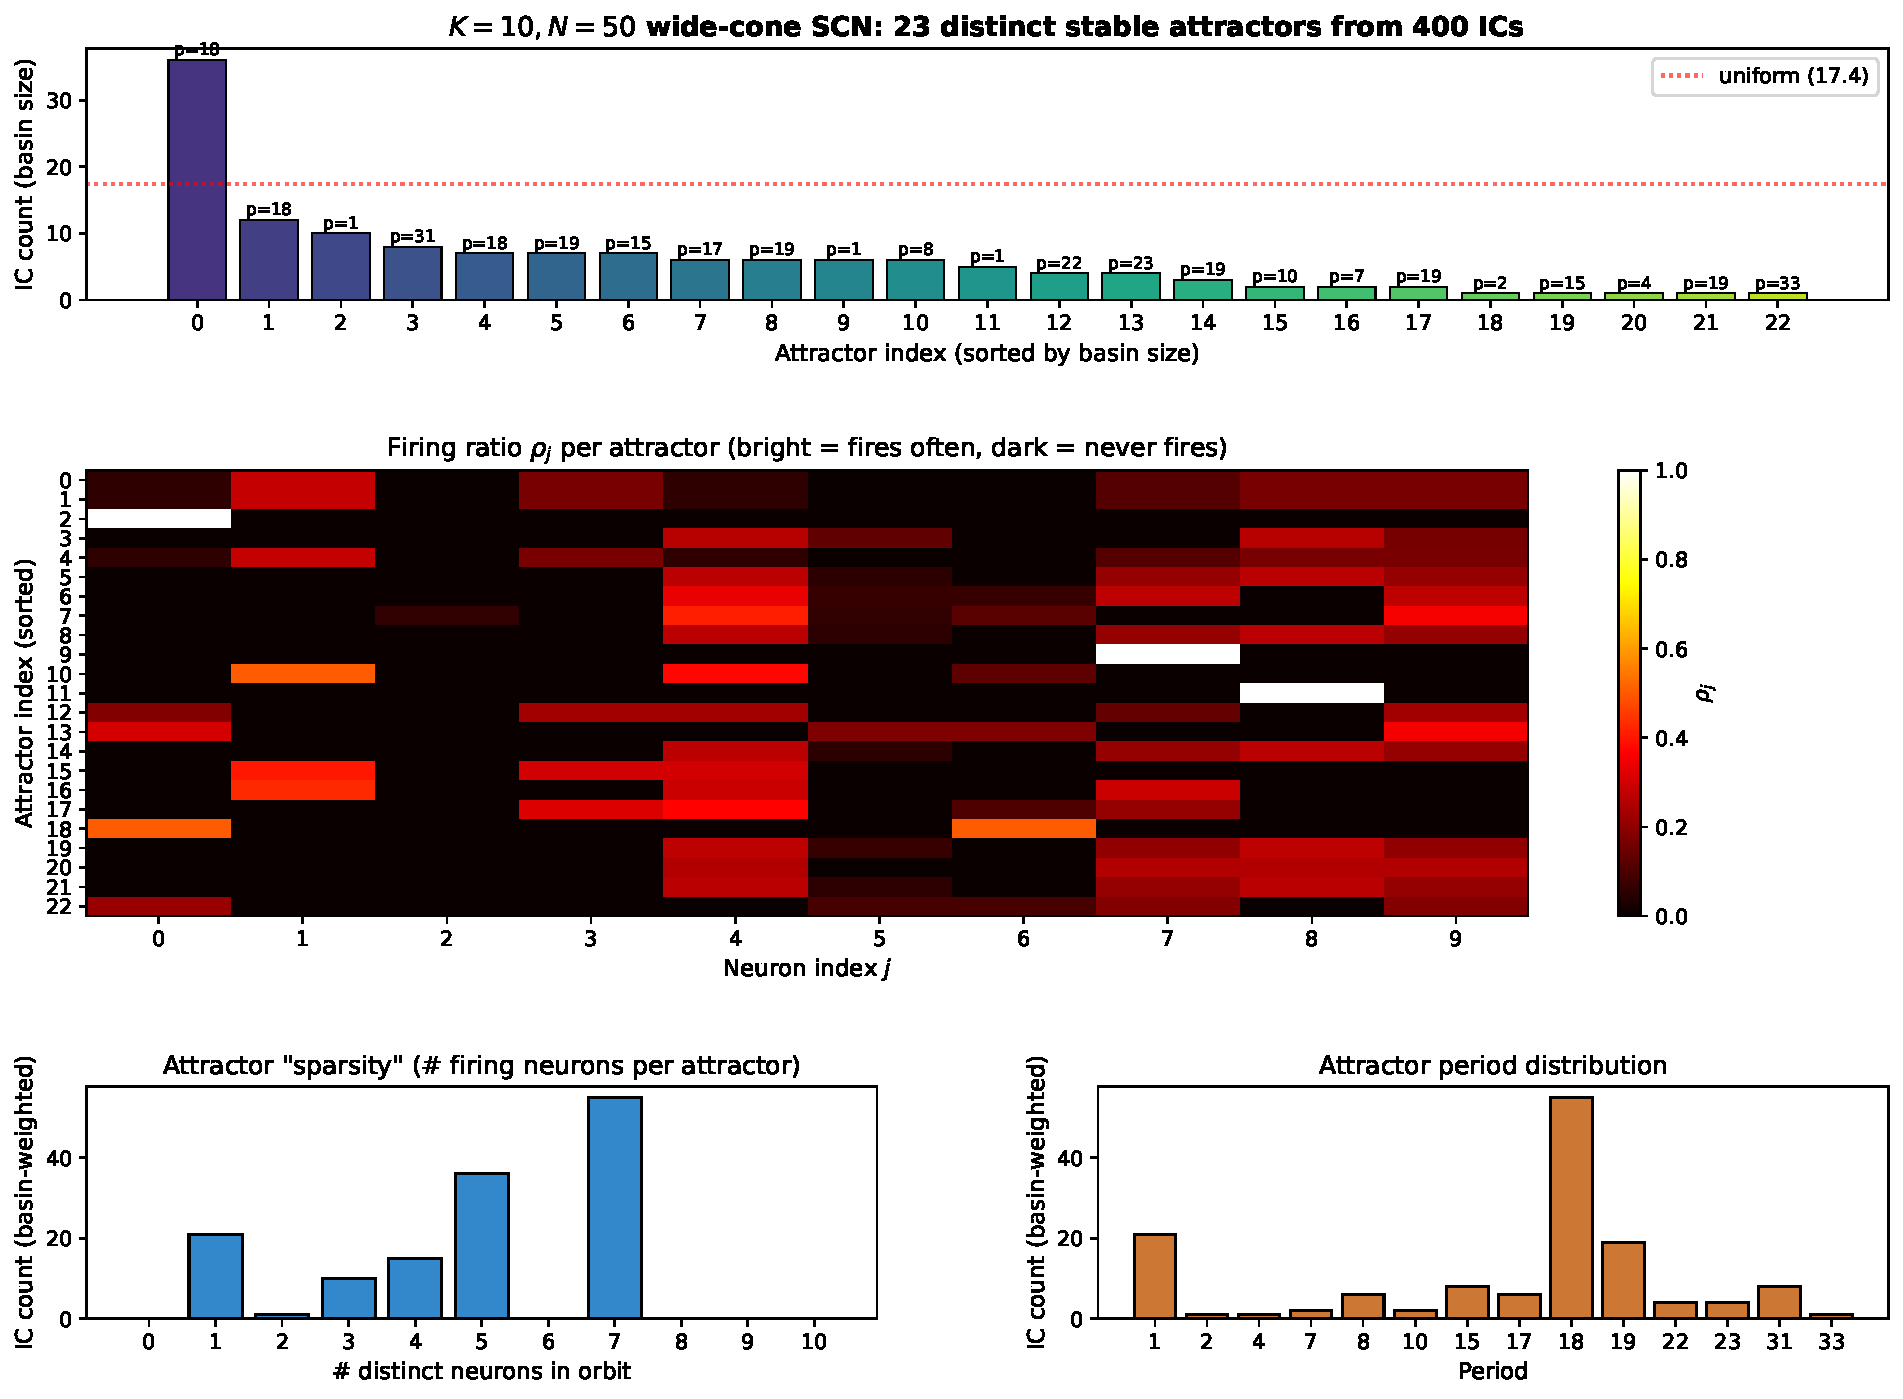
\includegraphics[width=\textwidth]{figures/multistability_highD}
\caption{Wide-cone $K=10$, $N=50$ SCN: basin survey over 400 random initial conditions reveals 23 distinct stable attractors. \textbf{Top:} basin size per attractor (sorted). \textbf{Middle:} firing-ratio $\rho_j$ per attractor (heatmap: attractor $\times$ neuron). Rows with identical rows share the same DC readout $\bar{\vv{y}}$ (spike-timing degeneracy compatible with Mancoo's readout uniqueness); distinct rows reveal genuine multistability at the readout level. \textbf{Bottom-left:} number of firing neurons per attractor. \textbf{Bottom-right:} attractor-period distribution. Complements Table~\ref{tab:wide-cone-atlas}, which lists the top~$8$ basins.}
\label{fig:multi-highD}
\end{figure}

\begin{figure}[ht]
\centering
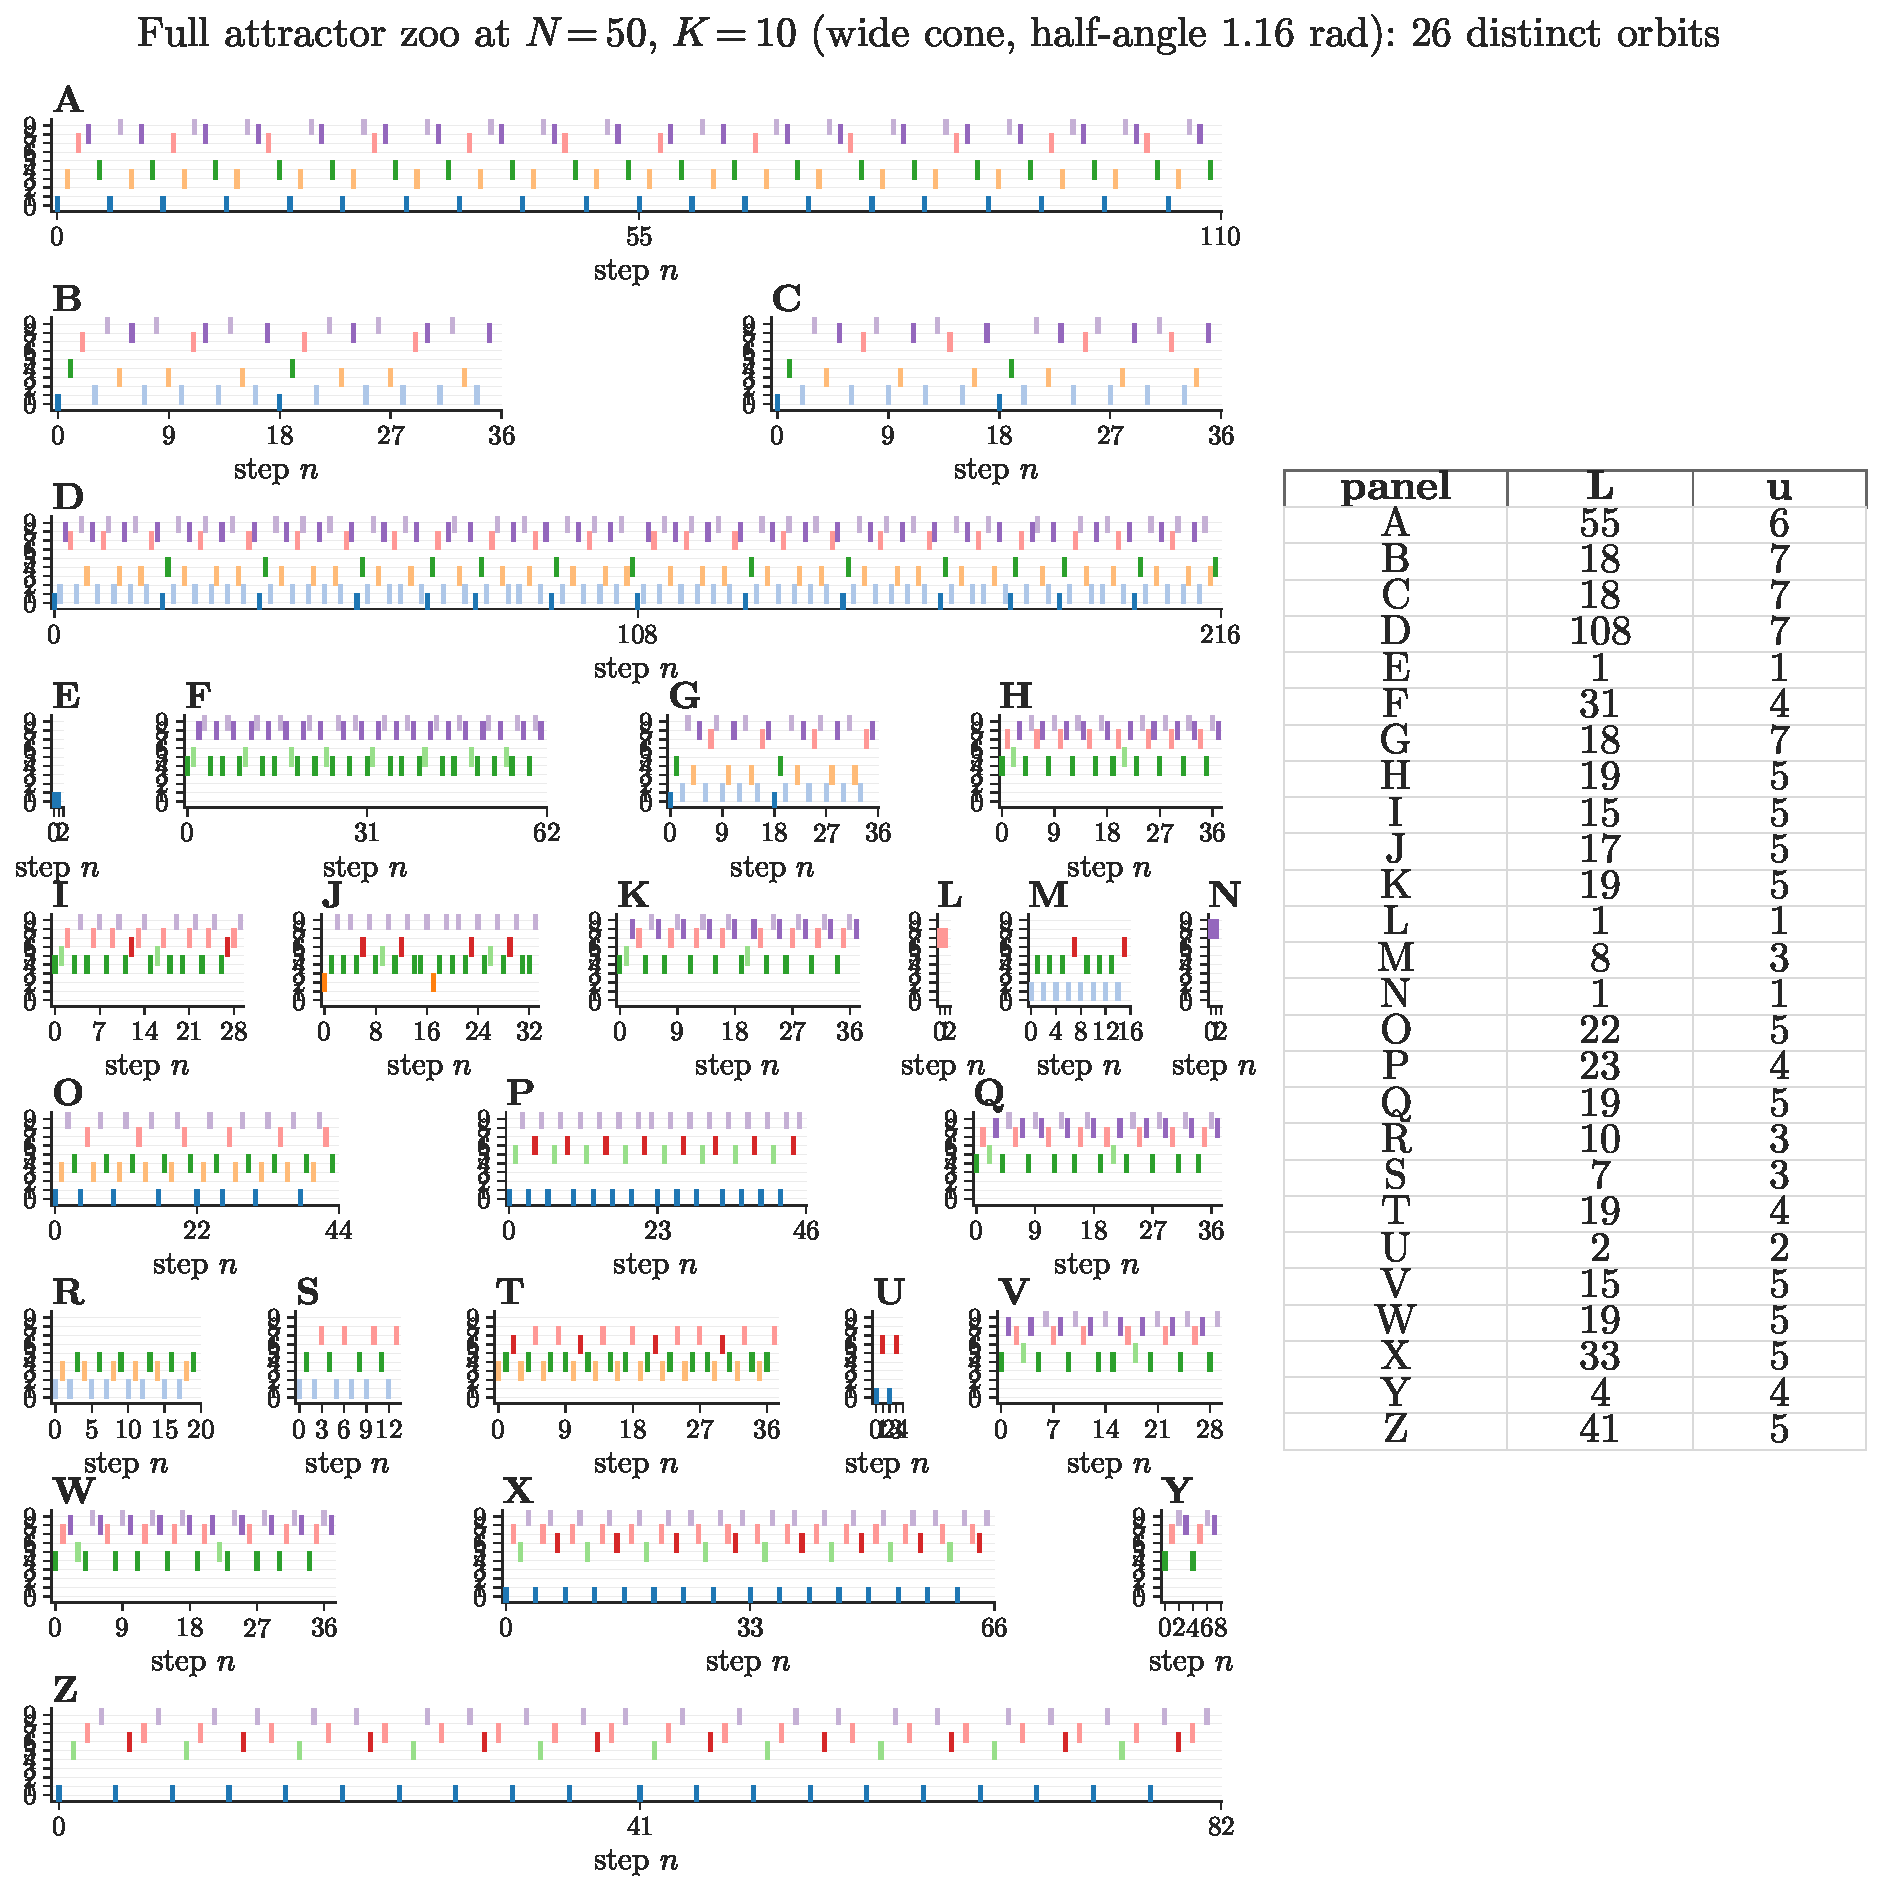
\includegraphics[width=\textwidth]{figures/orbit_zoo_wide_N50.pdf}
\caption{Full attractor zoo at $N{=}50$, $K{=}10$, half-angle $1.16$~rad: spike raster of every distinct stable periodic orbit found, with panel widths scaled to period. The $[\mathrm{S}]$ tag (``short'') marks orbits with period $p\leq 40$ discovered by the $400$-IC short-burn-in survey ($6\,000$ burn-in steps); the $[\mathrm{L}]$ tag (``long'') marks orbits with period $p\geq 33$ discovered only by the extended-burn-in pass ($20\,000$ burn-in steps) on basin-map cells that the short pass left unclassified.}
\label{fig:orbit-zoo-wide}
\end{figure}

\begin{figure}[ht]
\centering
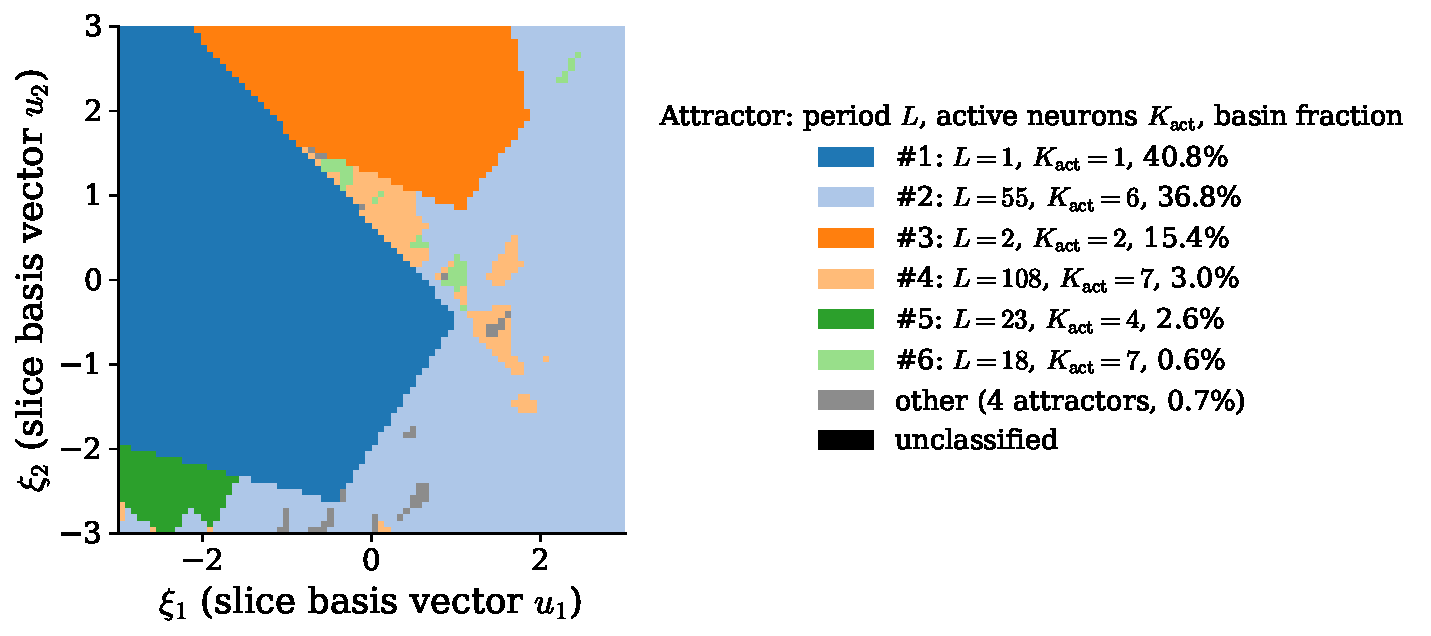
\includegraphics[width=0.75\textwidth]{figures/basin_map_wide.pdf}
\caption{Basin map of the wide-cone $N{=}50$, $K{=}10$ SCN (cone half-angle $1.16$~rad) on a random $2$D slice of the $49$-dimensional tangent space on $\mathcal{B}_1$: axes $\xi_1,\xi_2$ are coordinates in an orthonormal slice basis $(u_1,u_2)$; a point $(\xi_1,\xi_2)$ corresponds to the tangent state $\xi_1 u_1+\xi_2 u_2$. Each grid cell is coloured by the periodic attractor its orbit converges to (short- and long-period orbits merged); $10$ distinct attractors are resident on the slice. The $6$ largest basins are shown individually; the remaining $4$ are grouped as ``other''. Legend: $L$ is the period (letters per cycle) and $K_{\mathrm{act}}$ the number of distinct neurons that fire in the cycle. Every grid cell is classified — no diverging trajectories.}
\label{fig:basin-map-wide}
\end{figure}

\subsection{Self-transition runs}\label{app:self-trans}

A run of $k$ consecutive self-firings by neuron~$i$ contracts the tangent coordinate as $\xxi\mapsto(\alpha_i/(\alpha_i+1))^k\xxi$, pulling the orbit toward the foot $\xxi=\vv{0}$. Since the self-decay factor $c_i=\alpha_i/(\alpha_i+1)$ is constant (independent of $\xxi$), while the cross-transition factor $c_j=\alpha_j/(\DD_j^\top\yy^+)$ depends on $\xxi$ through the denominator, each self-firing shifts the relative ordering of the decay factors. The orbit self-fires until the contraction pushes $\xxi$ across a partition boundary (where $c_i=c_j$ for some $j\neq i$), at which point a cross-transition occurs. The run length is approximately $k \approx (\ln|\xxi_{\text{arrive}}| - \ln|\xxi_{\text{part}}|)/\ln((\alpha_i+1)/\alpha_i)$. Since self-transitions only contribute contractive factors $(\alpha_i/(\alpha_i+1))^k<1$ to the return map, words with longer self-transition runs are generically more stable.

\section{Analytical proofs and corollaries}\label{app:proofs}

\subsection{Birkhoff's ergodic theorem}\label{app:birkhoff}

We invoke the following classical result at several points in the main text (Section~\ref{sec:sturmian-chain}, Theorem~\ref{thm:cone}).

\begin{theorem}[Birkhoff's ergodic theorem]\label{thm:birkhoff}
Let $(X,\mathcal{F},\mu)$ be a probability space and let $T:X\to X$ be a measurable transformation that preserves $\mu$, i.e.\ $\mu(T^{-1}A)=\mu(A)$ for every $A\in\mathcal{F}$. For every $f\in L^1(\mu)$, the limit
\begin{equation}\label{eq:birkhoff}
\bar f(x)\;=\;\lim_{n\to\infty}\frac{1}{n}\sum_{k=0}^{n-1}f(T^kx)
\end{equation}
exists for $\mu$-almost every $x\in X$; the limit function $\bar f$ is $T$-invariant ($\bar f\circ T=\bar f$ $\mu$-a.e.); and $\int_X\bar f\,d\mu=\int_X f\,d\mu$. If in addition $T$ is \emph{ergodic} (every $T$-invariant set has measure 0 or 1), then $\bar f$ is constant $\mu$-a.e.\ and equals $\int_X f\,d\mu$; in particular, for any measurable set $A\in\mathcal{F}$,
\[
\lim_{n\to\infty}\frac{1}{n}\sum_{k=0}^{n-1}\mathbf{1}_A(T^kx)\;=\;\mu(A)\quad\text{for $\mu$-a.e.\ }x.
\]
\end{theorem}

The original references are \citet{birkhoff1931proof} and \citet{vonneumann1932proof} (mean ergodic theorem); modern textbook treatments include \citet{walters2000introduction} and \citet{petersen1983ergodic}. In our setting, $X=\Bsp_1\cup\{\infty\}$, $T=F_{\!\Bsp_1;\alpha_2}$ is the first-return piecewise-M\"obius map (Proposition~\ref{prop:circle-homeo}), $\mu=\mu_F$ is its unique invariant probability measure on the class-$\mathcal L$ side (which exists and is unique for orientation-preserving circle homeomorphisms with irrational rotation number; \citealp{herman1979conjugaison}), and the observable $f=\mathbf{1}_{P_2}$ is the indicator of the cross-transition cell. Applying~\eqref{eq:birkhoff} identifies the long-run firing ratio $\rho$ with the invariant mass $\mu_F(P_2)$, which is the identity used to align the SCN's partition with the rotation number in Section~\ref{sec:sturmian-chain}, Step~3.

\subsection{Vanishing Lyapunov exponent at irrational rotation number}\label{app:quasi-LE}

\begin{proposition}[Vanishing Lyapunov exponent at irrational rotation number, $K{=}2$]\label{prop:quasi-LE}
For the $K{=}N{=}2$ SCN in the cone-preserving regime ($\cos\psi>0$), let $F_{\alpha_2}$ be the first-return piecewise-M\"obius map (Proposition~\ref{prop:circle-homeo}) at drive $\alpha_2$ in the admissibility window, and suppose $\rho:=\rho(\alpha_2)$ is irrational. Call $\rho$ \emph{Diophantine of exponent~$\tau\geq 0$} if there exists $C>0$ such that $|\rho-p/q|\geq C\,q^{-2-\tau}$ for every rational $p/q$. Assume either of the following:
\begin{enumerate}[label=(\alph*),nosep]
    \item \emph{(Smooth case, Herman--Yoccoz)} $\rho$ is Diophantine and $F_{\alpha_2}$ is $C^2$ off its break point \citep{herman1979conjugaison,yoccoz1984conjugaison}.
    \item \emph{(Piecewise-M\"obius case, Liousse)} $\rho$ is Diophantine and the Boshernitzan invariant of the break-point derivative jump, $\log\bigl(F'(\xi_{\mathrm{part}}^+)/F'(\xi_{\mathrm{part}}^-)\bigr)$, satisfies the trivial-holonomy condition of \citet{liousse2005nombre} (which reduces to $F'(\xi_{\mathrm{part}}^+)=F'(\xi_{\mathrm{part}}^-)$ in the constant-slope case).
\end{enumerate}
Under either hypothesis the unique $F_{\alpha_2}$-invariant probability measure $\mu_F$ is absolutely continuous with respect to Lebesgue, and the Lyapunov exponent of the discrete return map satisfies
\begin{equation}\label{eq:LE-quasiperiodic}
\lambda(F_{\alpha_2},\mu_F) \;=\; \int_{\Bsp_1} \log|F'_{\alpha_2}(x)|\,d\mu_F(x) \;=\; 0.
\end{equation}
\end{proposition}

\begin{proof}
Let $f>0$ be the density of $\mu_F$ with respect to Lebesgue (existing under the AC hypothesis). $F_{\alpha_2}$-invariance, $\mu_F(F^{-1}(A))=\mu_F(A)$, gives the density-change equation
\[
f(F(x))\,|F'(x)| \;=\; f(x)
\]
for $\mu_F$-a.e.\ $x$. Taking logarithms,
\[
\log|F'(x)| \;=\; \log f(x) - \log f(F(x)),
\]
and integrating against $\mu_F$,
\[
\int\log|F'|\,d\mu_F \;=\; \int\log f\,d\mu_F - \int(\log f\circ F)\,d\mu_F \;=\; 0,
\]
where the last equality uses $F$-invariance of $\mu_F$ in the second integral.
\end{proof}

\paragraph{Discrete return-map LE vs.\ continuous-time flow LE.}
Equation~\eqref{eq:LE-quasiperiodic} gives the Lyapunov exponent of the \emph{discrete} return map $F$. The full continuous-time SCN flow on $\bigsqcup_i\Bsp_i$ has its own Lyapunov spectrum: it acquires one additional zero exponent in the time-translation direction (a generic property of any smooth limit-cycle-like dynamics, exploited as a working-memory substrate in \citealp{Park2023a}), while the discrete return map's transverse exponents $\log|\mu_k/\mu_1|<0$ become the flow's transverse exponents scaled by the average period. Both pictures give the same headline conclusion, $\lambda_{\max}=0$ at a quasi-periodic orbit, but via different mechanisms: measure preservation of the return map for the discrete picture, time-translation symmetry along the cycle for the flow picture.

\paragraph{Restriction to $K{=}2$.} Proposition~\ref{prop:quasi-LE} is stated only for $K{=}2$. For $K\geq 3$, the first-return map acts on a $(N{-}1)$-dimensional bound rather than a 1D circle; there is no single rotation number but a rotation \emph{vector} on a higher-dimensional torus, and the Herman--Liousse conjugacy theory generalises into the more delicate Yoccoz--Khanin framework for circle-of-tori maps. The corresponding zero-Lyapunov-exponent statement is not addressed here.

\subsection{Dale's-law geometry (proof sketch, kept for reference)}\label{app:dale-proof}

For a hypothetical Dale-compatible SCN under the connectivity $W_{ij}=-\DD_i^\top\DD_j$ (the main-text Dale-law paragraph is commented out; this proof sketch is retained for reference). If neuron $j$ is inhibitory, $W_{ij}=-\DD_i^\top\DD_j\leq 0$ for all~$i$, hence $\DD_i^\top\DD_j\geq 0$ for all~$i$. If neuron $k$ is excitatory, $W_{ik}=-\DD_i^\top\DD_k\geq 0$ for all~$i$, hence $\DD_i^\top\DD_k\leq 0$ for all~$i$. Taking $i=j$ (inhibitory): $\DD_j^\top\DD_k\leq 0$; taking $i=k$ (excitatory): $\DD_k^\top\DD_j\geq 0$. Both require $\DD_j^\top\DD_k=0$. Sign constraints within each population plus the classical result that at most $N+1$ unit vectors in $\RR^N$ can have all-negative pairwise inner products give the simplex bound $K_E\leq N+1$.

\subsection{Farey cascade to the singular parameter $\alpha_1^*$ for $\rho=1/\pi$}\label{app:pi-cascade}

For $K{=}N{=}2$ at $\psi=0.4\pi$, $\alpha_0=1$, the rotation number $\rho(\alpha_1)$ traces a complete devil's staircase (Section~\ref{sec:bifurcation}).
Irrational $\rho$ are achieved on a measure-zero set; we locate the singular $\alpha_1^*$ realizing $\rho=1/\pi$ by walking a Farey cascade of rational plateaus toward it.
The continued-fraction expansion of $1/\pi$ is $[0;3,7,15,1,292,\ldots]$, so the convergents are $1/3,7/22,106/333,113/355$, with semi-convergents $(7m{+}1)/(22m{+}3)$ filling the path from $7/22$ to $106/333$ as $m=1,\ldots,15$.

\paragraph{Method.}
For any rational $\rho=p/q$ with $\gcd(p,q)=1$, the unique balanced firing word is the mechanical Sturmian
$\sigma_{p/q}=(s_0,\ldots,s_{q-1})$ with $s_k=\lfloor(k{+}1)p/q\rfloor-\lfloor kp/q\rfloor\in\{0,1\}$.
Building the $2\times 2$ symbolic return matrix
$\vv{M}_\sigma(\alpha_1)=\prod_{k=q-1}^{0}\vv{M}_{s_{k+1}\leftarrow s_k}(\alpha_1)$ in $300$-digit \texttt{mpmath} and dehomogenizing its dominant eigenvector gives the predicted orbit $(\xi_0,\ldots,\xi_{q-1})$.
The orbit is realized iff the admissibility margin
\begin{equation}\label{eq:cascade-margin}
m(\alpha_1)\;=\;\min_{k}\Bigl(c_{s_{k+1}}-\!\!\max_{j\ne s_{k+1}}c_j\Bigr)
\end{equation}
is positive at the predicted orbit, where the decay factors $c_j=\alpha_j/(\DD_j^\top\yy_k^+)$ are evaluated at each post-spike readout~$\yy_k^+$. The plateau is then $\{\alpha_1:m(\alpha_1)>0\}$.

We bisect both edges of each plateau in turn, walking down the Farey chain:
the left bracket at level $(p_n,q_n)$ is the precisely refined right edge of $7/22$,
\[\alpha_1^{(7/22)\mathrm{R}}=0.5223343802940303852301165223341492397534560143394308644640508665058751\ldots\] (computed first at \texttt{mpmath} $\textsf{dps}=300$), and the right bracket is the previous level's left edge.

\begin{figure}[h]
\centering
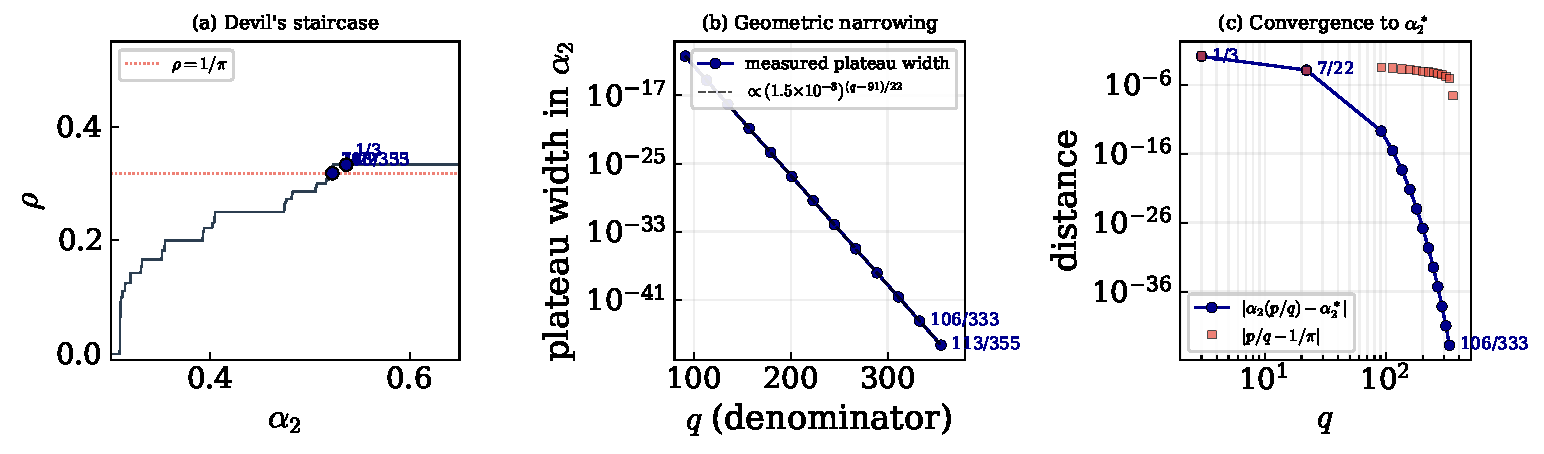
\includegraphics[width=0.95\textwidth]{figures/pi_approximants.pdf}
\caption{Farey cascade toward $\rho=1/\pi$. \textbf{(a)}~The devil's staircase with the four continued-fraction convergents marked. \textbf{(b)}~Plateau widths in $\alpha_1$ along the Farey chain decay geometrically by ${\sim}1.5\times 10^{-3}$ per step of $q$ by $22$. \textbf{(c)}~The plateau centres' distance to the cascade limit $\alpha_1^*$, alongside $|p/q-1/\pi|$ for comparison; both follow the same super-polynomial convergence.}
\label{fig:pi_approximants}
\end{figure}

\paragraph{Results.}
The 13~plateaus from $29/91$ down to the convergent $113/355$ all admit positive-width plateaus of unambiguously detectable width (Table~\ref{tab:cascade}, Figure~\ref{fig:pi_approximants}). Plateau widths decay geometrically by a factor of $\approx 1.5\times 10^{-3}$ per Farey step (each step adds $22$ to $q$), so the convergent $113/355$ has plateau width $4.95\times 10^{-47}$ in $\alpha_1$, far below the $10^{-16}$ double-precision floor that defeats simulation-based searches.

\begin{table}[h]
\centering
\begin{tabular}{rcc}
\hline
$\rho=p/q$ & $q$ & plateau width \\
\hline
$29/91$    &  91 & $3.99\times 10^{-13}$ \\
$36/113$   & 113 & $5.96\times 10^{-16}$ \\
$43/135$   & 135 & $8.91\times 10^{-19}$ \\
$50/157$   & 157 & $1.33\times 10^{-21}$ \\
$57/179$   & 179 & $1.99\times 10^{-24}$ \\
$64/201$   & 201 & $2.97\times 10^{-27}$ \\
$71/223$   & 223 & $4.45\times 10^{-30}$ \\
$78/245$   & 245 & $6.64\times 10^{-33}$ \\
$85/267$   & 267 & $9.93\times 10^{-36}$ \\
$92/289$   & 289 & $1.48\times 10^{-38}$ \\
$99/311$   & 311 & $2.22\times 10^{-41}$ \\
$106/333$  & 333 & $3.32\times 10^{-44}$ \\
$113/355$  & 355 & $4.95\times 10^{-47}$ \\
\hline
\end{tabular}
\caption{Plateau widths along the Farey cascade toward $\rho=1/\pi$, computed in \texttt{mpmath} at $300$-digit precision. Each step from $q$ to $q{+}22$ shrinks the plateau by ${\sim}1.5\times 10^{-3}$.}
\label{tab:cascade}
\end{table}

\paragraph{The singular point.}
Along the cascade, the right edge of $113/355$ and the left edge of $106/333$ coincide to all $\sim 80$~digits resolved in our run, giving the cascade limit
\begin{equation}
\alpha_1^*\;\approx\;0.522334380294030385230116522334149239753456014389052084833331820664863883\ldots
\end{equation}
This is the unique $\alpha_1$ at which the SCN has rotation number exactly $1/\pi$: the firing word is the aperiodic Sturmian $\sigma_{1/\pi}$ and the orbit closure has empty interior on $\Bsp_0$.

\paragraph{Irrational firing ratios are realized; finite-precision simulation only sees rational ones.}
The rotation number $\rho(\alpha_1)$ is continuous and monotone non-decreasing in $\alpha_1$ on this family (Section~\ref{sec:bifurcation}; \citealp{herman1979conjugaison}). It takes the value $0$ at small $\alpha_1$ and rises through $1/2$ at large $\alpha_1$. By the intermediate value theorem, $\rho$ attains \emph{every} real value in $[0,1/2]$ --- every rational, every algebraic and transcendental irrational --- so for each target $\omega\in[0,1/2]$ there exists $\alpha_1^*(\omega)$ realizing it.\footnote{Uniqueness up to plateau interior: for rational $\omega=p/q$, all $\alpha_1$ in the plateau realize $\omega$; for irrational $\omega$ the realization is at a single point.} Rational $\omega$ are realized on plateaus of positive Lebesgue measure; irrational $\omega$ are realized at single points forming a Cantor-like measure-zero set. The dynamics at every $\alpha_1$ is well defined --- deterministic update law, real-valued state, Birkhoff average converging to $\rho(\alpha_1)$ --- including at every irrational realization. What finite-precision simulation cannot do is \emph{set} $\alpha_1$ to a singular value: a double-precision $\alpha_1$ lies within $10^{-16}$ of its representable neighbour, and the plateaus have full Lebesgue measure in any region of the staircase, so round-off lands on a rational. Reaching $\alpha_1^*(1/\pi)$ requires the Farey cascade --- approaching the singular parameter from a sequence of computable rational neighbours at extended precision.

\paragraph{The cascade is the theory.}
$\alpha_1^*$ has no known closed-form expression --- the cascade itself is the canonical characterization. Three equivalent definitions all reduce to the same infinite procedure.

\emph{(i) As an inverse rotation number.} $\alpha_1^*$ is uniquely defined by $\rho(\alpha_1^*) = 1/\pi$, where the rotation number is the Birkhoff limit
\[
\rho(\alpha_1) \;=\; \lim_{n\to\infty} \frac{1}{n}\sum_{k=0}^{n-1} \mathbf{1}_{\{\text{neuron 1 fires at step } k\}}.
\]
Inverting a Birkhoff limit is itself an infinite procedure: $\alpha_1^*$ is a limit of limits.

\emph{(ii) As a topological conjugacy.} The natural rigidity statement is \textbf{Denjoy's theorem} \citep{denjoy1932courbes}: \emph{every orientation-preserving $C^2$ diffeomorphism $F$ of the circle with irrational rotation number $\rho$ is topologically conjugate to the rigid rotation $R_\rho(x)=x+\rho\pmod 1$ --- that is, there exists an orientation-preserving homeomorphism $h$ of the circle with $h\circ F\circ h^{-1}=R_\rho$} (see also \citealp{herman1979conjugaison}). The conjugacy is at most $C^0$, not analytic. Applied at $\alpha_1^*$ (rotation number $1/\pi$) it would give $F_{\alpha_1^*}$ conjugate to $R_{1/\pi}$. Two caveats. First, the SCN return map is continuous and piecewise M\"obius but only $C^0$ at the partition point $\xi_{\mathrm{part}}$, so the $C^2$ hypothesis of the classical theorem fails. Piecewise-smooth extensions \citep{liousse2005nombre} restore the conclusion provided no break point lies on the orbit closure; we do not verify this condition for the SCN, and record it as the natural sufficient hypothesis under which $\alpha_1^*$ corresponds to dynamics genuinely conjugate to rotation rather than to a Denjoy counter-example with a Cantor-set attractor. Second, in either case the conjugacy $h$ is at most $C^0$ and has no known closed-form expression, so it provides no analytic shortcut to $\alpha_1^*$.

\emph{(iii) As a constant defined by an infinite cascade.} A clean analogue is the \textbf{Feigenbaum bifurcation constant} of period-doubling: for a one-parameter family $f_r$ with a quadratic maximum (e.g.~the logistic map $f_r(x)=rx(1-x)$), let $r_1<r_2<\cdots$ be the parameter values at successive period-doubling bifurcations on the route to chaos. The ratio
\[
\delta \;=\; \lim_{n\to\infty}\frac{r_n-r_{n-1}}{r_{n+1}-r_n} \;\approx\; 4.66920160910299\ldots
\]
is a specific real number defined entirely by this limit and is universal across families with quadratic maxima \citep{feigenbaum1978quantitative}. No closed form is known for $\delta$; it is computable to arbitrary precision only by walking the cascade. Our $\alpha_1^*(1/\pi)$ is of the same character: a specific real number defined by an infinite Farey cascade, with no known closed form, computable only by walking the cascade to the required depth. Each Farey level here adds ${\sim}\log_{10}(1.5{\times}10^{-3})^{-1}\approx 2.8$ digits of $\alpha_1^*$; stopping at $113/355$ gives the ${\sim}50$ verified digits reported above. The next CF convergent $33102/103993$ has plateau width $\sim 10^{-1\,400}$, beyond any feasible computation.


\subsection{Chaos mechanism: stable but inadmissible periodic orbits}\label{app:chaos-mechanism}

In the chaotic regime ($\cos\psi_{\min}=-0.57$), every short periodic sub-word observed in the chaotic trajectory has a return map $\vv{M}_\sigma$ whose dominant eigenvector is mathematically \emph{stable} ($|\mu_2/\mu_1|<1$). For example, the word $(2,3)$ has $|\mu_2/\mu_1|=0.62$, word $(1,2)$ has $0.22$, word $(0,2)$ has $0.41$. Yet none of these fixed points are admissible: at some step in the candidate orbit, a different neuron would fire first. This pattern holds for all 30 most-visited sub-words of lengths 2--7.

The chaos therefore arises not because individual periodic orbits are unstable (they are all stable), but because the partition prevents the trajectory from settling into any of them. Each candidate orbit's fixed point lies outside the admissible region for its word, so the trajectory is perpetually deflected at partition boundaries. The piecewise switching between branches produces a net positive expansion ($\lambda_1=0.285$) even though each branch's own dynamics would be contracting.

This mechanism differs from smooth chaos (e.g.\ Smale horseshoes), where the attractor is woven from unstable periodic orbits. Here the periodic orbits exist with stable eigenvalues but are blocked by the combinatorial constraint of admissibility. The local Lyapunov (expanding) direction rotates across the attractor (standard deviation $88^\circ$, range $243^\circ$), confirming that no fixed direction is responsible for the expansion. Chaotic dynamics in neural circuits have been proposed as a substrate for probabilistic computation through sampling \citep{terada2024chaotic} and have been experimentally observed in cortical recordings \citep{korn2003there,sarbadhikari2001chaos}.

\paragraph{The algebraic machinery is regime-agnostic; only its meaning changes.}
The $\sigma\mapsto\vv{M}_\sigma\mapsto(\text{eigenvalues},\text{eigenvector}\mapsto\xi^*)$ construction is a polynomial-coefficient algebraic procedure that requires no positivity hypothesis and is therefore the same in both regimes. What changes are which guarantees still hold and what the predicted $\xi^*$ \emph{means} dynamically. Table~\ref{tab:cone-vs-chaos} summarizes.

\begin{table}[h]
\centering
\renewcommand{\arraystretch}{1.2}
\begin{tabular}{p{0.32\linewidth}p{0.28\linewidth}p{0.30\linewidth}}
\hline
\textbf{Property} & \textbf{Cone-preserving regime} ($\cos\psi_{ij}>0$ all $i,j$) & \textbf{Chaos regime} ($\cos\psi_{ij}<0$ some $i,j$) \\
\hline
$\vv{M}_\sigma$ construction & polynomial in parameters: same formula & polynomial in parameters: same formula \\
Dominant eigenvalue $\mu_1$ & simple, real, positive (Perron--Frobenius) & not guaranteed; can be complex pair, negative, or non-simple \\
Eigenvector in positive cone $\mathcal{C}$ & yes & not guaranteed \\
Hilbert-metric contraction $|\mu_k/\mu_1|<1$ & yes, uniform over orbit & breaks in general; can persist algebraically (as in our $K{=}4$ example) without giving an attractor \\
Admissibility of the $\sigma$-orbit at the predicted $\xi^*$ & one $\sigma$ admissible per parameter (locked on each plateau, Cor.~\ref{cor:within-plateau}) & generically fails for any short $\sigma$ observed in the trajectory: the predicted $\xi^*$ lies outside the partition cell of its own next firer \\
What the predicted $\xi^*$ is dynamically & the system's unique attracting periodic orbit & a (typically algebraically stable but \emph{inadmissible}) candidate that the trajectory perpetually deflects away from at partition boundaries \\
Source of complexity & smooth M\"obius branches; Arnold-tongue widths & partition-induced switching between branches; no fixed expanding direction \\
Number of admissible $\sigma$ at period $L$ & exactly one (the Sturmian $\sigma_{p/q}$ of the plateau) & system-dependent; in our example, no short admissible $\sigma$ is realized as a stable cycle \\
\hline
\end{tabular}
\caption{The eigenvector-orbit construction $\sigma\mapsto\xi^*$ runs identically in both regimes; what differs is which classical guarantees survive and what dynamical role the predicted $\xi^*$ plays.}
\label{tab:cone-vs-chaos}
\end{table}

\subsection{Robustness bound via eigenvector perturbation theory}\label{app:robustness}

For the RBYGYB orbit, the $3\times 3$ return map $\vv{M}_\sigma$ has right eigenvectors $\vv{u}_k$ and left eigenvectors $\vv{w}_k$ (normalized so $\vv{w}_k^\top\vv{u}_k=1$). Under a drive perturbation $\delta\alpha_j$, the return map shifts by $\delta\vv{M}=(\partial\vv{M}_\sigma/\partial\alpha_j)\delta\alpha_j$. The first-order eigenvector perturbation~\eqref{eq:eigpert} predicts the orbit shift $\delta\xxi^*$.

\textbf{Validation:} The predicted $\|\delta\xxi^*/\delta\alpha_j\|$ matches the numerically computed sensitivity to 4 significant figures for all four drives ($\text{ratio}\approx 1.000$), confirming the first-order theory is essentially exact.

\textbf{Tolerance bound:} The orbit survives perturbation $\delta\alpha_j$ iff the margin remains positive. The per-drive tolerance is $|\delta\alpha_j|_{\max}\approx m/|\partial m/\partial\alpha_j|$, where the margin gradient is computed by finite differences. Results:

\begin{center}
\begin{tabular}{lcccc}
\hline
Drive & $|\partial m/\partial\alpha|$ & Predicted tol.\ & Actual tol.\ & Ratio \\
\hline
$\alpha_1$ & 0.028 & 0.171 (8.4\%) & 0.051 (2.5\%) & 0.30 \\
$\alpha_2$ & 0.012 & 0.385 (18.8\%) & 0.029 (1.4\%) & 0.08 \\
$\alpha_3$ & 0.339 & 0.014 (0.6\%) & 0.014 (0.6\%) & 1.00 \\
$\alpha_4$ & 0.326 & 0.015 (0.6\%) & 0.015 (0.6\%) & 1.00 \\
\hline
\end{tabular}
\end{center}

The bound is tight for the most sensitive directions ($\alpha_3,\alpha_4$, where the margin gradient is large and the linearization is accurate) and conservative for the less sensitive directions ($\alpha_1,\alpha_2$, where higher-order curvature effects dominate). The eigenvector condition number $\kappa(\vv{S})=2.41$ confirms the return map is well-conditioned.




\section{Full remarks (condensed in main text)}\label{app:full-remarks}

\begin{remark}[Firing ratio vs.\ rotation number under this lift]\label{app-rem:rho-conventions}
Three quantities are attached to a period-$q$ orbit of the first-return map $F_{\!\Bsp_1}$ with $k$ cross-transitions (and $s=q{-}k$ self-transitions): the \emph{return-map rotation number} $\rho_F := k/q\in[0,1)$ under the cross-$+1$ lift (equivalently $s/q$ under the self-$+1$ lift used in the proposition above); the \emph{cross-transition fraction} $\rho_F = k/q$ (same quantity); and the \emph{spike-based firing ratio} $\rho_{\text{spike}} := k/(q{+}k) \in [0,1/2)$, the fraction of SCN spikes emitted by neuron~$2$. The three are related by a strictly monotone bijection $\rho_{\text{spike}}=\rho_F/(1+\rho_F)$ and parameterise the \emph{same} devil's staircase in $\alpha_2$ under different labelings; the rotation-number theorems of~\citet{rhodes1991topologies,alseda2000combinatorial} apply verbatim under any of these labelings. Throughout the paper we call $\rho:=\rho_F$ the ``firing ratio''; whenever a specific number appears (e.g.\ $\rho=2/7$ at the star in Fig.~\ref{fig:overview-supp}d) it is the spike-based quantity $\rho_{\text{spike}}$ (what \texttt{scn.py}'s \texttt{get\_firing\_ratios} returns for a periodic orbit). Endpoint statements ``$\rho\to 1$ as $\alpha_2 \text{ increases to } \alpha_1/\cos\psi \text{ from below}$'' refer to $\rho_F$; the corresponding $\rho_{\text{spike}}$ limit is $1/2$. When continued-fraction machinery is invoked (as in the $\rho=1/\pi$ cascade of Remark~\ref{rem:irrational} and Appendix~\ref{app:pi-cascade}), the natural labeling is $\rho_F$ because the CF expansion of $1/\pi$ selects semi-convergent plateaus at $\rho_F=p/q$; there we write $\rho_F$ explicitly.
\end{remark}

\begin{remark}[Irrational firing ratios and quasi-periodicity]\label{app-rem:irrational}
The rational plateaus of the devil's staircase (Theorem~\ref{thm:staircase}) cover the full $\alpha_2$ axis in the sense of Lebesgue measure (the staircase is \emph{complete}).
Irrational firing ratios, such as $\rho_F=1/\pi$, are achieved on a Cantor-like set of measure zero between the plateaus.
At these parameters, the orbit is quasi-periodic: the firing pattern never repeats and the trajectory is dense on the circle.
The singular parameter $\alpha_2^*$ that realizes a chosen irrational $\rho_F$ can nonetheless be located analytically as the limit of a Farey cascade of rational plateaus.
For $\rho_F=1/\pi$ we walk the semi-convergents $(7m{+}1)/(22m{+}3)$ of the continued-fraction expansion $[0;3,7,15,1,292,\ldots]$ and find that the plateau widths shrink geometrically by a factor ${\sim}1.5\times 10^{-3}$ per step of $q$ by~$22$, from $3.99\times 10^{-13}$ at $\rho_F=29/91$ down to $4.95\times 10^{-47}$ at the convergent $\rho_F=113/355$.
This places $\alpha_2^*\approx 0.522334380294030385230116522334149239753456014389052\ldots$, accurate to ${\sim}50$~digits and well beyond the double-precision floor that defeats forward simulation.
The full procedure is in Appendix~\ref{app:pi-cascade}.
\end{remark}

\begin{remark}[Connection to periodically driven oscillators]\label{app-rem:driven-oscillators}
The devil's staircase structure is analogous to the mode-locking observed in periodically driven neural oscillators \citep{glass1988clocks}, where the driving frequency plays the role of $\alpha_2$.
The key difference is that our staircase arises from the intrinsic dynamics under constant input (the drive $\alpha_2$ sets the geometry, not a time-varying forcing), and the projective structure provides exact analytical control over each plateau.
\end{remark}

\begin{remark}[Sturmian structure of firing words]\label{app-rem:sturmian}
For $K=2$ in the cone-preserving regime $\cos\psi>0$, the realizable finite firing words are exactly the \emph{mechanical Sturmian} sequences $\sigma_{p/q}$ (Christoffel words; periodic-balanced binary words), one per rational rotation number $p/q\in(0,1)$ \citep{lothaire2002algebraic}: binary sequences in which, for any two subwords of the same length, the neuron-$2$ count differs by at most~$1$.
This is equivalent to the symbolic dynamics of a circle rotation by $\rho\in(0,1)$ (Morse--Hedlund coding).
The characterization means every realizable word is ``as uniform as possible'' given its rational firing ratio, a strong constraint that is a direct consequence of the circle-homeomorphism structure. At the singular parameter $\alpha_2^*(\omega)$ realising an irrational $\omega$, the firing word is a genuine (aperiodic) classical Sturmian sequence; the mechanical Sturmians of continued-fraction convergents of $\omega$ converge to it in the shift-space product topology (see Appendix~\ref{app:pi-cascade} for the explicit $\omega=1/\pi$ construction).
\end{remark}

\begin{remark}[Why higher $K$ is qualitatively different]\label{app-rem:K-geq-3-richer}
The proof above is special to $K{=}2$: the encoding partition has 2 cells, and Morse--Hedlund~\citep{morse1938symbolic,morse1940symbolic} forces 2-cell rotation encodings to be Sturmian (Theorem~\ref{thm:classification}). For $K\geq 3$ the partition has $K$ cells, the three-distance theorem no longer applies in the same way, and the realizable firing-word class becomes much larger, allowing higher-dimensional balanced and quasi-balanced sequences from the projective dynamics on $\bigsqcup_i\Bsp_i$. A precise characterization of realizable words for $K\geq 3$ is open; we treat it heuristically via the inverse problem (Section~\ref{sec:inverse}) rather than via a classification theorem and offer the following conjecture as the natural structural target.
\end{remark}

\begin{remark}[Quasi-periodic orbits are not chaotic]\label{app-rem:quasi-vs-chaos}
At measure-zero parameters where the firing ratio is irrational, the orbit is \emph{quasi-periodic}: our first-return map is a piecewise-M\"obius orientation-preserving circle homeomorphism, hence of bounded variation, so by Denjoy's theorem it is conjugate to a rigid rotation \citep[Thm.~11.2.7 and Thm.~12.1.1]{katok1995introduction} and has maximal Lyapunov exponent zero (Proposition~\ref{prop:quasi-LE} in Appendix~\ref{app:quasi-LE}). Chaos requires at least one $\cos\psi_{ij}<0$, which breaks the cone and admits positive Lyapunov exponents. Both regimes are deterministic; the qualitative distinction lies in finite-precision predictability, which fails only in the chaotic regime above the precision horizon $n\sim\lambda_{\max}^{-1}\log(1/\varepsilon)$ \citep{ott2002chaos}.
\end{remark}

\begin{remark}[Word impossibility from decoder alignment]\label{app-rem:impossible}
Two neurons with $\cos\psi_{ji}\approx 1$ cannot fire consecutively (the large projection makes bound~$j$ reached last, not first).
\end{remark}


%%%%%%%%%%% APPENDED: classical-defs section (auto-inserted) %%%%%%%%%%%


\section{Formal statements of the classical results used}\label{app:classical-defs}

This appendix collects the formal statements of the classical mathematical results the main paper invokes by name. Each block is compact and self-contained; the main text 
ef{}'s these labels wherever the corresponding name-drop appears.

\subsection{Positive cone and Birkhoff-Hilbert contraction}\label{sec:supp:hilbert}

% ---------------------------------------------------------------
% Supplementary block: Birkhoff-Hilbert contraction on a positive cone.
% Referenced from the main text via \ref{thm:supp:birkhoff-hilbert}.
% ---------------------------------------------------------------

\begin{definition}[Positive decoder cone]\label{def:supp:positive-cone}
Given decoder vectors $\{\DD_j\}_{j=1}^{N}\subset\RR^{N}$, the \emph{open positive cone} cut out by the decoder inequalities is
\[
\mathcal{C} \;=\; \bigl\{\,\vv{y}\in\RR^{N} : \DD_j^\top\vv{y}>0 \ \text{for all } j=1,\dots,N\,\bigr\}.
\]
$\mathcal{C}$ is open, convex, salient, and closed under $\RR_{>0}$-scaling, so it descends to a projective cone $\mathcal{C}/\RR_{>0}$ on the space of rays.
\end{definition}

\begin{definition}[Hilbert projective metric]\label{def:supp:hilbert}
For $\vv{y},\vv{z}\in\mathcal{C}$, put
\[
M(\vv{y},\vv{z})=\max_{1\le j\le N}\frac{\DD_j^\top\vv{y}}{\DD_j^\top\vv{z}}, \qquad m(\vv{y},\vv{z})=\min_{1\le j\le N}\frac{\DD_j^\top\vv{y}}{\DD_j^\top\vv{z}}.
\]
The \emph{Hilbert projective (semi-)metric} on $\mathcal{C}$ is
\[
d_H(\vv{y},\vv{z}) \;=\; \log\!\bigl(M(\vv{y},\vv{z})/m(\vv{y},\vv{z})\bigr)\ge 0,
\]
which vanishes iff $\vv{y}\parallel\vv{z}$ and is a genuine metric on the ray quotient $\mathcal{C}/\RR_{>0}$ (classical; see the modern exposition around projective contractions in the general framework of \citealt{rhodes1991topologies}).
\end{definition}

\begin{theorem}[Birkhoff cone contraction; classical]\label{thm:supp:birkhoff-hilbert}
Let $A:\RR^{N}\to\RR^{N}$ be linear with $A\bigl(\overline{\mathcal{C}}\setminus\{\vv{0}\}\bigr)\subset\mathcal{C}$ (strict cone invariance), and let
\[
\Delta \;=\; \sup_{\vv{u},\vv{v}\in A(\mathcal{C})} d_H(\vv{u},\vv{v}) \;<\;\infty
\]
be the projective diameter of the image cone. Then $A$ is a strict $d_H$-contraction:
\[
d_H(A\vv{y},A\vv{z}) \;\le\; \tanh\!\bigl(\Delta/4\bigr)\, d_H(\vv{y},\vv{z}) \qquad \forall\,\vv{y},\vv{z}\in\mathcal{C},
\]
with Lipschitz constant $\tanh(\Delta/4)<1$. In particular, $A$ has a unique fixed ray in $\mathcal{C}$ and every orbit in $\mathcal{C}/\RR_{>0}$ converges to it geometrically (Birkhoff, 1957; classical).
\end{theorem}

\begin{corollary}[Return-map contraction for SCN itineraries]\label{cor:supp:scn-birkhoff}
Assume all pairwise decoder cosines are positive, $\DD_j^\top\DD_i>0$ for every $i,j$. Then each SCN transition matrix $\vv{M}_{j\leftarrow i}$ maps $\overline{\mathcal{C}}\setminus\{\vv{0}\}$ into $\mathcal{C}$, and hence, for any admissible periodic itinerary $\sigma=(i_0,i_1,\dots,i_p=i_0)$, the return map
\[
\vv{M}_\sigma \;=\; \vv{M}_{i_p\leftarrow i_{p-1}}\cdots\vv{M}_{i_1\leftarrow i_0}
\]
is a strict $d_H$-contraction by Theorem~\ref{thm:supp:birkhoff-hilbert}. Consequently $\vv{M}_\sigma$ admits a unique fixed ray $\vv{y}_\sigma^\star\in\mathcal{C}$, and every admissible periodic orbit of the symbolic system is asymptotically stable.
\end{corollary}

\subsection{Sturmian sequences}\label{sec:supp:sturmian}

\begin{definition}[Mechanical Sturmian sequence]\label{def:supp:sturmian}
Fix coprime integers $p,q\in\mathbb{N}$ with $\gcd(p,q)=1$ and set $\rho=p/q\in(0,1)$. The \emph{mechanical Sturmian} (or Christoffel) word of slope $\rho$ is
\[
  \sigma_{p/q}=(s_0,s_1,\ldots,s_{q-1})\in\{0,1\}^q,\qquad s_k \;=\; \Bigl\lfloor \tfrac{(k+1)p}{q}\Bigr\rfloor-\Bigl\lfloor \tfrac{kp}{q}\Bigr\rfloor,
\]
extended $q$-periodically to a bi-infinite sequence. Equivalently, $\sigma_{p/q}$ is the itinerary of $0$ under the rigid rotation $R_\rho:\theta\mapsto\theta+\rho\pmod{1}$ with respect to the length-$\rho$ arc partition $\{[0,1-\rho),[1-\rho,1)\}$ of the circle $\RR/\mathbb{Z}$ \citep{morse1938symbolic,lothaire2002algebraic}.
\end{definition}

\begin{definition}[Bi-infinite Sturmian sequence]\label{def:supp:sturmian-inf}
A bi-infinite sequence $\vv{s}\in\{0,1\}^{\mathbb{Z}}$ is \emph{Sturmian} if, for every $n\ge 1$, the number of distinct length-$n$ factors of $\vv{s}$ equals exactly $n+1$. Equivalently, $\vv{s}$ is the coding of an irrational rotation $R_\rho$ ($\rho\in(0,1)\setminus\mathbb{Q}$) by a length-$\rho$ arc partition of $\RR/\mathbb{Z}$; the mechanical words $\sigma_{p/q}$ are the periodic ($\rho\in\mathbb{Q}$) case and any irrational Sturmian is a limit of the mechanical words $\sigma_{p_n/q_n}$ associated to the continued-fraction convergents $p_n/q_n\to\rho$ \citep{morse1940symbolic,lothaire2002algebraic}.
\end{definition}

\begin{theorem}[Sturmian = balanced binary]\label{thm:supp:sturmian-balanced}
A binary word $\vv{s}\in\{0,1\}^{\mathbb{Z}}$ is Sturmian if and only if it is \emph{balanced}, i.e., for every pair of factors $u,v$ of $\vv{s}$ with $|u|=|v|$, one has $\bigl||u|_1-|v|_1\bigr|\le 1$, where $|w|_1$ denotes the number of $1$s in $w$. In particular, the mechanical words $\sigma_{p/q}$ are exactly the periodic balanced binary words, and their slope $\rho=p/q$ coincides with the asymptotic density of $1$s \citep{coven1973sequences,lothaire2002algebraic}.
\end{theorem}

\subsection{Morse-Hedlund coding of a rotation}\label{sec:supp:morse-hedlund}

\begin{definition}[Morse--Hedlund coding of a rotation]\label{def:supp:morse-hedlund-coding}
Let $R_\rho:S^1\to S^1$, $x\mapsto x+\rho\pmod 1$, be the rigid rotation by $\rho\in[0,1)$, and let $\{I_0,I_1\}$ be the two-cell partition $I_0=[0,1-\rho)$, $I_1=[1-\rho,1)$ (any length-$\rho$ arc and its complement will do). The \emph{Morse--Hedlund coding} of the orbit of $x_0\in S^1$ is the one-sided sequence
\[
\sigma(x_0)\;=\;(s_0,s_1,s_2,\ldots)\in\{0,1\}^{\mathbb{N}},\qquad s_k\;=\;\mathbf{1}_{I_1}\!\bigl(R_\rho^{k}(x_0)\bigr),
\]
so that $s_k$ records which cell of the partition contains the $k$-th iterate \citep{morse1940symbolic,lothaire2002algebraic}.
\end{definition}

\begin{theorem}[Morse--Hedlund complexity of rotation codings]\label{thm:supp:morse-hedlund}
Let $\sigma(x_0)$ be the coding of Definition~\ref{def:supp:morse-hedlund-coding} and let $p_n(\sigma):=\#\{\text{distinct factors of length }n\text{ in }\sigma\}$ be its factor-complexity function.
\begin{enumerate}[leftmargin=1.5em,itemsep=2pt]
    \item If $\rho\notin\mathbb{Q}$, then for every $x_0$ the sequence $\sigma(x_0)$ is \emph{Sturmian}, i.e.\ it is aperiodic and
    \[
        p_n(\sigma)\;=\;n+1\qquad\text{for all } n\ge 0.
    \]
    \item If $\rho=p/q$ in lowest terms, then $\sigma(x_0)$ is purely periodic with period $q$, and for generic $x_0$ it coincides with the mechanical (rational Sturmian) word $\sigma_{p/q}$ defined by $s_k=\lfloor (k+1)p/q\rfloor-\lfloor kp/q\rfloor$.
\end{enumerate}
Conversely, every Sturmian sequence arises, up to a choice of intercept, as a coding of some irrational rotation \citep{morse1938symbolic,morse1940symbolic,lothaire2002algebraic}.
\end{theorem}

\begin{remark}
The main text invokes Definition~\ref{thm:supp:morse-hedlund} when identifying the SCN's next-firer partition with a rotation-aligned coding: the identity of the neuron that spikes at step $k$ plays the role of $s_k$, so the low-complexity growth $p_n=n+1$ (irrational $\rho$) or eventual $q$-periodicity (rational $\rho$) is exactly the symbolic signature the network inherits from the underlying rotation.
\end{remark}

\subsection{The Rhodes--Thompson class $\mathcal{L}$ and rotation numbers of piecewise-monotone circle maps}
\label{sec:supp:rhodes-thompson}

\begin{definition}[The class $\mathcal{L}$]\label{def:rhodes-thompson-class}
Let $\mathcal{L}$ denote the set of maps $\widetilde F:\RR\to\RR$ such that (i) $\widetilde F$ is non-decreasing, (ii) $\widetilde F(x+1)=\widetilde F(x)+1$ for all $x\in\RR$, and (iii) $\widetilde F$ is upper semi-continuous. Each $\widetilde F\in\mathcal{L}$ is the lift of a (possibly discontinuous) degree-$1$ non-decreasing circle map $F:\mathcal{C}/\mathbb{Z}\to\mathcal{C}/\mathbb{Z}$; jump discontinuities are permitted \citep{rhodes1991topologies}.
\end{definition}

\begin{definition}[Rotation number]\label{def:rotation-number}
For $\widetilde F\in\mathcal{L}$ the \emph{rotation number} is
\[
\rho(\widetilde F)\;:=\;\lim_{n\to\infty}\frac{\widetilde F^{n}(x)-x}{n}\pmod 1 ,
\]
which exists and is independent of $x\in\RR$ \citep{poincare1885courbes,rhodes1991topologies}.
\end{definition}

\begin{theorem}[Rhodes--Thompson, extending Poincar\'e]\label{thm:supp:rhodes-thompson}
Equip $\mathcal{L}$ with the sup-norm topology $\|\widetilde F_1-\widetilde F_2\|_\infty=\sup_{x\in[0,1]}|\widetilde F_1(x)-\widetilde F_2(x)|$. Then $\rho:\mathcal{L}\to[0,1]$ is continuous and monotone in $\widetilde F$. Moreover, for any one-parameter family $\{\widetilde F_\alpha\}\subset\mathcal{L}$ depending monotonically and continuously on $\alpha$, the map $\alpha\mapsto\rho(\widetilde F_\alpha)$ is a \emph{devil's staircase}: each rational value $p/q\in\mathbb{Q}\cap[0,1]$ is attained on a closed interval (possibly a point) of $\alpha$, and each irrational value is attained at a unique $\alpha$ \citep{rhodes1991topologies,alseda2000combinatorial,herman1979conjugaison}.
\end{theorem}

\begin{remark}[Application to the SCN first-return map]\label{rem:supp:scn-rhodes}
For $K=2$ the SCN first-return map $F_{\!\Bsp_0;\alpha_1}$ on the boundary arc admits a degree-$1$ lift $\widetilde F_{\alpha_1}$ that is piecewise a M\"obius restriction and, by the cone-contraction argument of the main text, non-decreasing with at most one jump per fundamental domain. Hence $\widetilde F_{\alpha_1}\in\mathcal{L}$, and Theorem~\ref{thm:supp:rhodes-thompson} applied to the family $\alpha_1\mapsto\widetilde F_{\alpha_1}$ yields the staircase structure of $\rho(\alpha_1)$ asserted in Theorem~\ref{thm:staircase}.
\end{remark}

\subsection{Davis-Kahan eigenvector perturbation}\label{sec:supp:davis-kahan}

\begin{theorem}[Davis-Kahan eigenvector perturbation, non-symmetric analogue]\label{thm:supp:davis-kahan}
Let $\vv{M}\in\RR^{N\times N}$ have simple eigenvalue $\mu_1$ with right eigenvector $\vv{u}_1$ and left eigenvector $\vv{w}_1^\top$ normalised by $\vv{w}_1^\top\vv{u}_1=1$, and let $\{(\mu_k,\vv{u}_k,\vv{w}_k^\top)\}_{k=2}^{N}$ denote the remaining biorthogonal eigen-triples ($\vv{w}_j^\top\vv{u}_k=\delta_{jk}$). Under a perturbation $\delta\vv{M}$ with $\|\delta\vv{M}\|$ small compared to the spectral gap $|\mu_1-\mu_2|$, the leading right eigenvector shifts, to first order, by
\begin{equation}
\delta\vv{u}_1 \;=\; \sum_{k=2}^{N}\frac{\vv{w}_k^\top(\delta\vv{M})\vv{u}_1}{\mu_1-\mu_k}\,\vv{u}_k,
\end{equation}
so that, writing $\vv{S}=[\vv{u}_1\mid\cdots\mid\vv{u}_N]$ for the right-eigenvector matrix and $\kappa(\vv{S})=\|\vv{S}\|\|\vv{S}^{-1}\|$ for its condition number,
\begin{equation}
\|\delta\vv{u}_1\| \;\lesssim\; \frac{\kappa(\vv{S})}{|\mu_1-\mu_2|}\,\|\delta\vv{M}\|.
\end{equation}
This is the non-normal generalisation of the classical symmetric $\sin\theta$ theorem \citep{davis1970rotation}, obtained by replacing orthogonal projectors onto invariant subspaces by oblique (biorthogonal) ones; see \citep[Chapter V]{stewart1990matrix}. Applied to the SCN slow map, it is exactly the tolerance bound~\eqref{eq:tolerance} controlling how far the orbit-defining leading eigenvector of $\vv{M}$ may drift under parameter perturbations.
\end{theorem}

\subsection{Arnold tongues and the devil's staircase (general)}\label{sec:supp:arnold}

\begin{theorem}[Arnold tongues and the devil's staircase]\label{thm:supp:arnold-tongue}
Let $\{F_\alpha\}_{\alpha\in[0,1]}$ be a one-parameter family of orientation-preserving degree-$1$ circle homeomorphisms $F_\alpha:S^1\to S^1$ depending continuously and (weakly) monotonically on $\alpha$, and let $\rho(F_\alpha)\in[0,1]$ denote the Poincar\'e rotation number. Assume the family is nontrivially nonlinear (i.e.\ not conjugate to a rigid-rotation family). Then:
\begin{enumerate}
\item[(i)] \emph{Mode locking.} For every rational $p/q\in[0,1]\cap\mathbb{Q}$ the level set $I_{p/q}:=\{\alpha\in[0,1]:\rho(F_\alpha)=p/q\}$ is a closed interval of strictly positive Lebesgue measure, $|I_{p/q}|>0$; these Arnold tongues cover a full-measure open dense subset $\Bsp\subset[0,1]$.
\item[(ii)] \emph{Devil's staircase.} The map $\alpha\mapsto\rho(F_\alpha)$ is continuous, nondecreasing, and locally constant on $\Bsp$, hence a Cantor function. Irrational rotation numbers are attained on the residual Lebesgue-null Cantor set $[0,1]\setminus\Bsp$.
\item[(iii)] \emph{Farey ordering.} If $p/q,\,p'/q'\in\mathbb{Q}$ are Farey neighbours, $|pq'-p'q|=1$, then the tongue at the mediant $(p+p')/(q+q')$ lies strictly between $I_{p/q}$ and $I_{p'/q'}$, and its width scales as $|I_{(p+p')/(q+q')}|=O(1/q_{\max}^{2})$ with $q_{\max}=q+q'$ in the near-linear regime \citep{arnold1961small}.
\end{enumerate}
\end{theorem}

\noindent This is Arnold's classical result on small denominators for circle diffeomorphisms \citep{arnold1961small}; the residual-Cantor characterisation of the irrational locus and its zero measure follow from Denjoy--Herman theory \citep{herman1979conjugaison}. In the main text we apply (i)--(ii) to the induced circle map on the SCN's invariant loop to obtain the plateau widths in Theorem~\ref{thm:staircase}, and use the Farey $1/q^{2}$ scaling of (iii) as the quantitative form of the mediant prediction stated in the Discussion.


%%%%%%%%%%% END APPENDED %%%%%%%%%%%
 so all cross-references resolve
% internally.

\newcommand{\vv}[1]{\mathbf{#1}}
\newcommand{\DD}{\vv{D}}
\newcommand{\yy}{\vv{y}}
\newcommand{\xx}{\vv{x}}
\newcommand{\xxi}{\boldsymbol{\xi}}
\newcommand{\RR}{\mathbb{R}}
\newcommand{\CC}{\mathbb{C}}
\newcommand{\Bsp}{\mathcal{B}}
\newcommand{\BoA}{\operatorname{BoA}}
\newcommand{\tr}{\mathrm{tr}}

\newtheorem{definition}{Definition}
\newtheorem{proposition}{Proposition}
\newtheorem{lemma}{Lemma}
\newtheorem{theorem}{Theorem}
\newtheorem{corollary}{Corollary}
\newtheorem{remark}{Remark}
\newtheorem{example}{Example}
\newtheorem{conjecture}{Conjecture}

\title{Spike Coding Networks as Piecewise Projective Maps:\\
Closed-Form Stable Periodic Firing Patterns and Connectivity for Working Memory}
\author{Anonymous authors\\
    Affiliation withheld for double-blind review\\
    \texttt{anonymous@example.org}\\
}

\begin{document}
\maketitle

\begin{abstract}
Spike coding networks (SCNs) model neural populations whose collective firing approximates a target signal. We show that under constant input, the spike-and-decay dynamics of an SCN reduces to a discrete map whose state lives on the boundaries triggering each spike. The map is matrix-valued: every spike corresponds to multiplication by a small fixed matrix, and every periodic firing pattern is the dominant eigenvector of the matrix product along its cycle. The orbit positions, the per-cycle contraction rates, and the criterion for stability are then read off in closed form from a single eigendecomposition. The geometry of the decoders controls global behaviour through a single sign. When all pairwise decoder cosines are positive (the SCN connectivity is then uniformly inhibitory), the map preserves a positive cone and contracts in the Hilbert metric, so every realised orbit is stable and the firing ratio traces a complete devil's staircase as a function of any drive. When at least one pairwise cosine is negative, cone preservation fails and the same algebraic machinery generates positive topological entropy and chaos. We solve the single-word inverse problem, finding network parameters that realise one prescribed firing pattern as a stable orbit, by recasting it as a semi-algebraic feasibility question with a differentiable admissibility margin. In examples the resulting networks are multistable: several distinct firing patterns coexist as stable limit cycles at the same parameters, with the initial state determining which orbit is realised. The framework also yields a quantitative account of behavioural sequence-memory capacity through the admissibility margin's systematic decrease with sequence length.
\end{abstract}

%======================================================================
\section{Introduction}\label{sec:intro}
%======================================================================

Recurrent spiking neural networks produce rich temporal dynamics, but their analysis is typically limited to simulation or mean-field approximations. Spike coding networks (SCNs), introduced by \citet{boerlin2013predictive} as a framework for efficient neural coding, offer a structured alternative: their dynamics are constrained by a readout equation that ties each neuron's spiking to a geometric threshold condition on a set of hyperplanes. Between spikes the readout decays exponentially toward the origin, and when it crosses one of these hyperplanes the corresponding neuron fires and the readout jumps back into the interior. As we show, this alternation of decay and threshold crossing is exactly reducible to a \emph{piecewise projective map} on the hyperplanes: composing successive spike-then-decay steps corresponds to matrix multiplication, and each periodic firing pattern appears as an eigenvector of the resulting matrix product.

The analytical tractability of this reduction opens the door to a class of problems that are inaccessible in general spiking networks. As a motivating example, consider \emph{sequence working memory}: an animal hears a melody, watches a sequence of colored lights, or plans a sequence of motor actions, and must hold this temporal pattern in mind for later recall. A recurrent network can in principle store such a sequence as a periodic attractor, i.e.\ a limit cycle whose firing pattern encodes the sequence. But demonstrating this requires answering three questions:
\begin{enumerate}[nosep]
    \item \textbf{Forward:} given a network, what periodic firing patterns does it produce?
    \item \textbf{Inverse:} given a desired sequence, can we construct a network that produces it?
    \item \textbf{Stability:} are the resulting orbits robust to perturbation and noise?
\end{enumerate}
For a general spiking network, all three questions require numerical simulation, but for the SCN we provide \emph{analytical} answers.


\begin{enumerate}[nosep]
    \item We derive the \emph{piecewise projective map} that exactly governs SCN dynamics: each spike-then-decay step is an $N\times N$ matrix acting projectively, compositions are matrix products, and periodic orbits are eigenvectors (Section~\ref{sec:map}). Applied to the parameter dependence, this reveals a \emph{devil's staircase} bifurcation structure, complete when decoder cosines are positive, with genuine chaos emerging when at least one pairwise cosine is negative (Section~\ref{sec:bifurcation}).
    \item We solve the inverse problem by introducing the \emph{admissibility margin}, a continuous objective whose positivity is equivalent to a target firing word being realized, enabling gradient-based optimization (Section~\ref{sec:inverse}).
\end{enumerate}

 The spike coding network framework was introduced in the context of predictive efficient coding \citep{boerlin2011spike,boerlin2013predictive,deneve2016efficient}, with the underlying geometric threshold conditions developed in parallel \citep{barrett2013firing,chalk2016neural} and recently extended to excitatory-inhibitory architectures with latent boundaries \citep{podlaski2024approximating}; the notation in this paper follows the latter for consistency. Complementary lines of work show that the same efficient-coding substrate can be trained to implement universal spike-based computation \citep{thalmeier2016spikes} and admits closed-form optimal control laws for linear plants \citep{slijkhuis2024closedform}. Our closed-form results are of the intrinsic-dynamics kind, characterising which \emph{autonomous} periodic firing patterns are storable in an SCN under constant input rather than which external control signals steer it. Our cone-preserving regime ($\cos\psi_{ij}>0$ for every pair) coincides with the inhibition-dominated, stable-boundary regime studied by \citet{calaim2022geometry}, who showed numerically that this regime supports robust ``boundary computation'' and self-correcting trajectories. We provide an analytical explanation of why this regime is special: positive cosines force the projective return map to contract the Hilbert metric on the positive cone, which rules out chaos and forces every admissible periodic orbit to have $|\mu_k/\mu_1|<1$ (Theorem~\ref{thm:cone}). The mixed-excitation/inhibition framework of \citet{podlaski2024approximating} extends the SCN to networks that approximate arbitrary linear computations $\xx\mapsto\vv{A}\xx + \vv{b}$ via stable boundary trajectories; their construction implicitly requires the boundary to be \emph{globally attracting}, which is exactly the cone-preserving condition (positive cosines $\Leftrightarrow$ Hilbert contraction $\Leftrightarrow$ globally attracting boundary). In their cone-preserving subset, every linear computation supported by their construction is realised by a stable periodic SCN orbit whose eigenvector position $\xxi^*_\sigma$ (and full Lyapunov spectrum $\{|\mu_k/\mu_1|\}_{k=2}^N$) we predict in closed form (Theorem~\ref{thm:eigvec}). The negative-cosine permits-chaos regime of Theorem~\ref{thm:cone}(b) corresponds to the portion of \citet{podlaski2024approximating}'s framework where the boundary becomes piecewise linear with unstable faces; the linear-computation guarantee then survives only when the trajectory is steered by external input away from these unstable directions, an operating condition we make geometric via the partition margins~\eqref{eq:partition}.

Event-based spike maps that propagate the network state analytically from one spike to the next have been developed for general spiking networks \citep{monteforte2010dynamical,monteforte2012dynamic}: full Lyapunov spectra of large balanced networks were obtained in the first, and ``dynamic flux tubes'' (stable trajectories surrounded by exponentially separating basins) were identified in networks of LIF neurons in the second. Analytical single-spike Jacobians for arbitrary network topologies were derived by \citet{engelken2013dynamical}; Lyapunov spectrum analysis was extended to rate networks in \citep{engelken2023lyapunov}; and efficient event-based simulation and training algorithms for sparse spiking networks are available in \citep{engelken2023sparseprop}. These works operate in the full $K$-dimensional membrane-potential space, where the spike-to-spike map is a general nonlinear function and orbits must be found by simulation. The contribution of the present paper is to show that the SCN's exponential decay mechanism endows this map with \emph{projective} structure: the state reduces to $(N{-}1)$-dimensional tangent coordinates on which the map is a ratio of affine functions, compositions are matrix products, and periodic orbits are eigenvectors (Theorem~\ref{thm:eigvec}). Analytical orbit prediction, stability analysis, and the inverse problem then follow without simulation.

Mode-locking and Arnold-tongue structures~\citep{arnold1961small} (Theorem~\ref{thm:supp:arnold-tongue}) in periodically \emph{forced} integrate-and-fire oscillators have been studied since at least \citep{coombes1999mode}, including a derivation of Lyapunov exponents for the firing map \citep{coombes1999liapunov}. In that setting the devil's staircase arises from the interaction between the neuron's intrinsic period and an external forcing frequency. The staircase described here is qualitatively different: it arises from the \emph{intrinsic} dynamics of a multi-neuron network under constant input, with mode-locking occurring between neurons rather than between a neuron and an external clock. The single-neuron stability condition $|\mu_2/\mu_1|<1$ (Theorem~\ref{thm:eigvec}) of \citep{coombes1999liapunov} generalises in our setting to the multi-neuron projective return map $\vv{M}_\sigma$, whose eigenvalue ratios give the full Lyapunov spectrum in closed form.

Discrete-time maps arising in spiking networks have also been considered more generally \citep{cessac2010overview}, though without exploiting the projective structure specific to the SCN decay mechanism. Balanced networks of excitatory and inhibitory neurons \citep{brunel2000dynamics} support reliable spatiotemporal computation \citep{pyle2017spatiotemporal} and, in the tightly-balanced limit, admit an optimisation reading as minimax dynamics \citep{li2020minimax}; strong inhibitory signalling has separately been identified as the mechanism behind stable temporal dynamics and working memory in trained spiking networks \citep{kim2021strong}, and learning algorithms for target-driven recurrent spiking dynamics have been developed \citep{kim2018learning}. Sequence generation in recurrent networks has been modelled via synfire chains \citep{abeles1991corticonics}, heteroclinic cycles \citep{rabinovich2008transient}, task-trained RNNs \citep{sussillo2009force,sussillo2013blackbox,maheswaranathan2019universality}, and, in spiking substrates, structured sequence-learning-and-replay circuits \citep{bouhadjar2022sequence}, with low-rank structure increasingly used to interpret the resulting dynamics \citep{barak2017recurrent,driscoll2024flexible,vyas2020ctd}. These approaches provide powerful computational models but lack the exact analytical tractability of the projective-map framework. The behavioural working-memory capacity limit of $4\pm 1$ items \citep{cowan2001magical} has been linked to electrophysiological sequence representations in prefrontal cortex \citep{averbeck2002parallel} and hippocampus \citep{baeg2003dynamics}; a mechanistic account of this limit through the shrinking admissibility margin (Section~\ref{sec:apps-simon}) is given here.


%======================================================================
\section{The piecewise projective map}\label{sec:map}
%======================================================================

In this section, we establish the core mathematical framework of our approach by translating the continuous-time SCN dynamics into a discrete-time representation. By leveraging the geometric properties of the network's state space, we reduce the continuous trajectory in $\RR^N$ to a closed-form, \textbf{piecewise projective map} operating on the $(N-1)$-dimensional neuron bounds. This dimensional reduction provides the exact analytical tractability needed to solve for periodic orbits, derive explicit stability criteria, and map state-space partitions without relying on numerical simulation. For a complete summary of our symbols and conventions, see Table~\ref{tab:notation} in the supplementary material.

\subsection{SCN setup}\label{sec:setup}

We follow the spike coding network (SCN) framework of \citet{boerlin2013predictive,podlaski2024approximating}. Consider $K$ leaky integrate-and-fire neurons encoding a constant input $\xx\in\RR^N$. Each neuron~$i$ has membrane potential
\begin{equation}\label{eq:voltage}
    V_i = \DD_i^\top\xx - \DD_i^\top\yy,
\end{equation}
where $\DD_i\in\RR^N$ is neuron~$i$'s \textbf{decoder} (a unit vector, $\|\DD_i\|=1$, specifying its ``preferred direction'' in signal space), and $\yy(t)\in\RR^N$ is the network \textbf{readout}:
\begin{equation}\label{eq:readout}
    \yy(t) = \vv{D}\,\vv{r}(t),\qquad \vv{D}=[\DD_2\;\cdots\;\DD_K]\in\RR^{N\times K},
\end{equation}
with $\vv{r}(t)\in\RR^K$ the filtered spike trains satisfying $\dot{\vv{r}}=-\lambda\vv{r}+\vv{s}(t)$, where $\lambda>0$ is the (uniform) synaptic leak rate and $\vv{s}(t)=\sum_{k}\delta(t-t_k)\vv{e}_{i_k}$ collects the spike events (a Dirac train on the $i_k$-th unit vector at each firing time $t_k$). The first term in~\eqref{eq:voltage} is a feedforward drive from the input (analogous to $F_i x$ in \citealt{podlaski2024approximating}); the second is recurrent feedback from the readout (analogous to $E_i y$). The recurrent connectivity is
\begin{equation}\label{eq:connectivity}
    W_{ij} = -\DD_i^\top\DD_j,
\end{equation}
which is \emph{negative} when decoders point in similar directions ($\cos\psi_{ij}>0$, inhibitory) and \emph{positive} when they oppose ($\cos\psi_{ij}<0$, excitatory). The sign of the pairwise decoder cosine thus determines whether the connection obeys Dale's law for inhibition.

Between spikes the readout decays exponentially toward the origin; when neuron~$i$ fires, the readout jumps by $\DD_i$:
\begin{equation}\label{eq:dynamics}
    \text{decay: }\;\yy(\tau)=e^{-\lambda\tau}\yy^+,\qquad
    \text{spike: }\;\yy\mapsto\yy+\DD_i.
\end{equation}
Neuron~$i$ fires when $V_i\geq T_i$, i.e.\ $\DD_i^\top(\xx-\yy)\geq T_i$, which we rewrite as the readout reaching the \emph{spike bound}
\begin{equation}\label{eq:bound}
    \Bsp_i = \bigl\{\yy\in\RR^N : \DD_i^\top\yy=\alpha_i\bigr\},\qquad \alpha_i\coloneqq\DD_i^\top\xx-T_i.
\end{equation}
Each $\Bsp_i$ is a hyperplane with normal~$\DD_i$; the scalar $\alpha_i>0$ is the \emph{suprathreshold drive}.\footnote{Sign convention. We take $\alpha_i>0$ to mean neuron~$i$ is suprathreshold, matching \citet{calaim2022geometry,podlaski2024approximating}. The original Boerlin--Deneve--Machens formulation \citep{boerlin2013predictive} writes the firing condition as $V_i>T_i$ with $V_i=\DD_i^\top(\xx-\hat\xx)-\tfrac{1}{2}\|\DD_i\|^2$ and $T_i$ absorbing a constant offset; our $\alpha_i$ is their $V_i-T_i$ evaluated at $\hat\xx=\vv{0}$, so both conventions agree that firing corresponds to the same suprathreshold half-space and differ only in whether the sign is folded into the definition of the threshold.} Geometrically, the readout $\yy$ lives inside the polyhedron bounded by the spike bounds; it decays toward the origin until it hits a bound, triggering a spike that pushes it back into the interior. The full trajectory is a sequence of spike-then-decay steps, each mapping a point on one spike bound to a point on another, forming a \emph{discrete-time map on the spike bounds}.


Throughout the paper we analyse the SCN in its \emph{autonomous} form (fixed drives $\boldsymbol\alpha$), equivalent to a Boerlin--Deneve--Machens autoencoder~\citep{boerlin2013predictive,bourdoukan2012learning,barrett2016optimal} driven by constant input $\vv{x}$, since a spike coding network's suprathreshold drive is $\alpha_i = \DD_i^\top\vv{x} - T_i$. Constant $\vv{x}$ therefore reduces to constant $\boldsymbol\alpha$. \citet{mancoo2020understanding} show that the \emph{ideal} SCN (a convex-QP solver) has a unique readout $\bar{\vv{y}}^*$ for any input; the greedy spike-selection dynamics we analyse is a heuristic descent that can converge to different limit cycles depending on initial condition (Section~\ref{sec:apps-wm}), with uniqueness at the \emph{readout} level: all coexisting limit cycles share the same time-averaged $\bar{\vv{y}}$ (e.g., all chirality orbits of Section~\ref{sec:apps-wm} produce $\bar{\vv{y}}=\tfrac{1}{3}\sum_j\DD_j$).


\subsection{Coordinates on a spike bound}\label{sec:coords}

Since every spike event maps the readout onto a spike bound, and the decay between spikes is just a straight line (a ray toward the origin), the full dynamics reduce to a sequence of points on bounds. We therefore need a coordinate system on each bound.

Each spike bound $\Bsp_i$ is an $(N{-}1)$-dimensional hyperplane in $\RR^N$. We parameterize it by choosing an orthonormal basis $\vv{U}_i\in\RR^{N\times(N-1)}$ for the tangent space $\DD_i^\perp$, satisfying $\vv{U}_i^\top\vv{U}_i=\vv{I}_{N-1}$ and $\vv{U}_i^\top\DD_i=\vv{0}$. Together with the normal, this gives a complete basis: $\DD_i\DD_i^\top + \vv{U}_i\vv{U}_i^\top = \vv{I}_N$. Any point on~$\Bsp_i$ then decomposes as
\begin{equation}\label{eq:tangent}
    \yy = \underbrace{\alpha_i\,\DD_i}_{\text{foot}} + \underbrace{\vv{U}_i\,\xxi}_{\text{tangent displacement}},\qquad \xxi=\vv{U}_i^\top\yy\in\RR^{N-1}.
\end{equation}
The \textbf{foot} $\alpha_i\DD_i$ is the point on $\Bsp_i$ closest to the origin along the normal direction, at distance $\alpha_i$ from the origin. The \textbf{tangent coordinate} $\xxi\in\RR^{N-1}$ encodes where on the bound the readout sits, and is the state variable of the discrete map. This achieves a key dimension reduction: the continuous-time ODE in $\RR^N$ becomes a discrete map on $(N{-}1)$-dimensional coordinates.


\subsection{The transition map}\label{sec:transition}

We now derive the discrete map that takes a position $\xxi$ on bound~$i$ (just before neuron~$i$ fires) to a position $\xxi'$ on bound~$j$ (the next bound hit after decay). This is the central calculation of the paper: it turns the continuous spike-and-decay dynamics into an algebraic map. The six panels of Figure~\ref{fig:derivation} track the construction geometrically and mirror Steps 1--5 below.

\begin{figure}[!ht]
\centering
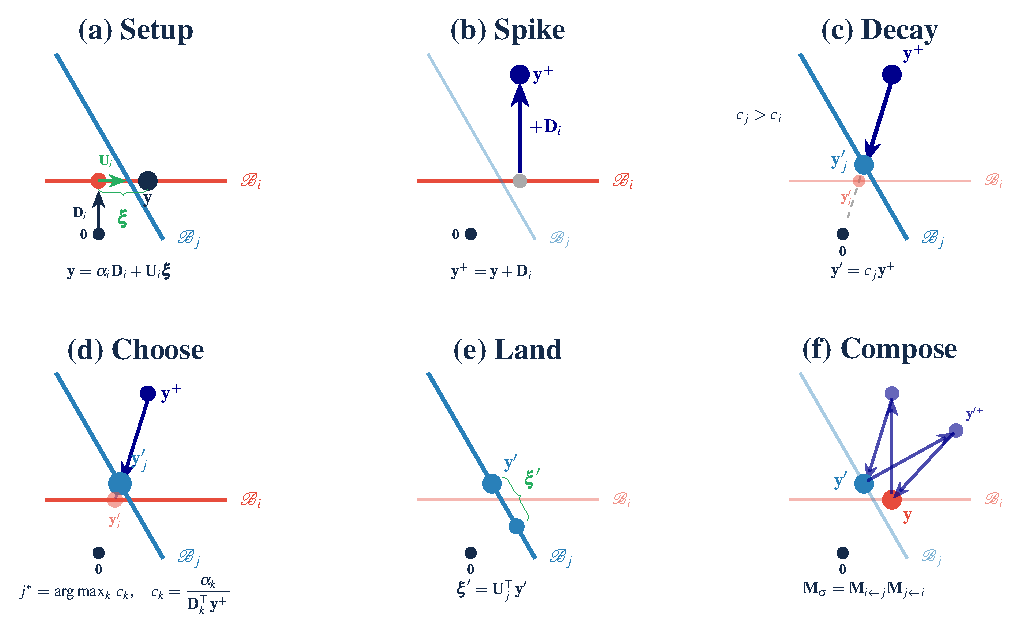
\includegraphics[width=\textwidth]{figures/derivation_tikz.pdf}
\caption{Geometric derivation of the transition map $\vv{M}_{j\leftarrow i}$ (Steps 1--5 of the main text) for a period-2 orbit between $\Bsp_i$ (red) and $\Bsp_j$ (blue).
\textbf{(a)}~State $\yy=\alpha_i\DD_i+\vv{U}_i\xxi$ on $\Bsp_i$.
\textbf{(b)}~Spike: $\yy\mapsto\yy^+=\yy+\DD_i$.
\textbf{(c)}~Decay $e^{-\lambda\tau}\yy^+$; each candidate $k$ has decay factor $c_k=\alpha_k/(\DD_k^\top\yy^+)$.
\textbf{(d)}~The largest $c_k$ wins ($j^*=\arg\max_k c_k$); here $\yy'_j$ on $\Bsp_j$ is reached first.
\textbf{(e)}~Project onto the bound-$j$ frame: $\xxi'=\vv{U}_j^\top\yy'_j$.
\textbf{(f)}~Two steps close the orbit; $\vv{M}_\sigma=\vv{M}_{i\leftarrow j}\vv{M}_{j\leftarrow i}$.}
\label{fig:derivation}
\end{figure}

The key geometric insight is that exponential decay $\yy(\tau) = e^{-\lambda\tau}\yy^+$ moves the readout along a \emph{ray toward the origin}. Hitting the hyperplane $\DD_j^\top\yy = \alpha_j$ determines a unique scale factor $c_j = \alpha_j/(\DD_j^\top\yy^+) \in (0,1)$, so the landing point is $\yy' = c_j\,\yy^+$. This ratio of inner products is what makes the map \textbf{projective}: the landing coordinates depend on the \emph{direction} of $\yy^+$ from the origin, not its magnitude.

\emph{Step 1: Spike.} Starting from $\yy=\alpha_i\DD_i+\vv{U}_i\xxi$ on bound~$i$, neuron~$i$ fires and the readout jumps by $\DD_i$:
\begin{equation}\label{eq:post-spike}
    \yy^+ = \yy+\DD_i = (\alpha_i+1)\DD_i + \vv{U}_i\xxi.
\end{equation}
The post-spike readout $\yy^+$ is now \emph{above} all spike bounds (inside the polyhedron), at distance $\alpha_i+1$ from the origin along the $\DD_i$ direction, with the same tangent displacement $\xxi$.

 \emph{Step 2: Decay.} The readout decays along the ray $\yy(\tau)=e^{-\lambda\tau}\yy^+$ toward the origin (with $\tau\geq 0$ the elapsed time since the last spike). It hits bound~$j$ (the condition $\DD_j^\top\yy = \alpha_j$) at decay factor $c_j = \alpha_j/(\DD_j^\top\yy^+)$:
\begin{equation}\label{eq:decay}
    \yy' = c_j\,\yy^+ = \frac{\alpha_j}{\DD_j^\top\yy^+}\;\yy^+.
\end{equation}
The bound hit first (smallest $\tau$, equivalently largest $c_j$) determines which neuron fires next: $j^* = \arg\max_j c_j$ among active neurons ($\alpha_j > 0$). This is the \emph{partition} of the state space into regions, one per possible next neuron.

\emph{Step 3: New coordinates.} Projecting the landing point onto the tangent frame of bound~$j$:
\begin{equation}\label{eq:xiprime}
    \xxi' = \vv{U}_j^\top\yy' = \frac{\alpha_j\;\vv{U}_j^\top\yy^+}{\DD_j^\top\yy^+}.
\end{equation}
As written, both numerator and denominator depend on $\yy^+$; we now expand them in terms of the tangent coordinate~$\xxi$.

\emph{Step 4: Inter-bound geometry.} To write this explicitly, define the geometric quantities relating bounds $i$ and $j$:
\begin{equation}\label{eq:geometry}
    \cos\psi_{ji}=\DD_j^\top\DD_i,\quad
    \vv{v}_{ji}=\vv{U}_i^\top\DD_j\in\RR^{N-1},\quad
    \vv{w}_{ji}=\vv{U}_j^\top\DD_i\in\RR^{N-1},\quad
    \vv{R}_{ji}=\vv{U}_j^\top\vv{U}_i\in\RR^{(N-1)\times(N-1)}.
\end{equation}
Here $\cos\psi_{ji}$ is the angle between decoder directions, $\vv{v}_{ji}$ projects $\DD_j$ into the tangent space of bound~$i$ (needed for the denominator), $\vv{w}_{ji}$ projects $\DD_i$ into the tangent space of bound~$j$ (needed for the numerator), and $\vv{R}_{ji}$ maps tangent vectors from bound~$i$'s frame into bound~$j$'s frame (not a rotation in general, since the two tangent spaces $\DD_i^\perp$ and $\DD_j^\perp$ do not coincide).

 The subscript $_{ji}$ on each of $\cos\psi$, $\vv{v}$, $\vv{w}$, $\vv{R}$ orders ``destination first, source second'' to match the transition $\Bsp_i\to\Bsp_j$, but the role of $\vv{U}_i$ versus $\vv{U}_j$ on the \emph{left} of each definition depends on which tangent frame the quantity acts in: $\vv{R}_{ji}$ and $\vv{w}_{ji}$ produce outputs in the new (bound-$j$) tangent frame, so they carry $\vv{U}_j^\top$ on the left; $\vv{v}_{ji}$ appears in the denominator $\DD_j^\top\yy^+$ which is evaluated at a state still parameterized by the old (bound-$i$) tangent coordinate $\xxi$, so $\vv{v}_{ji}$ carries $\vv{U}_i^\top$ on the left.

Expanding:
\begin{align}
    \DD_j^\top\yy^+ &= (\alpha_i+1)\cos\psi_{ji}+\vv{v}_{ji}^\top\xxi,\label{eq:denom}\\
    \vv{U}_j^\top\yy^+ &= (\alpha_i+1)\vv{w}_{ji}+\vv{R}_{ji}\xxi.\label{eq:numer}
\end{align}
Both expressions are affine in~$\xxi$, so the map~\eqref{eq:xiprime} is a \emph{rational linear function} of~$\xxi$ (a ratio of affine maps).

\emph{Step 5: The transition map.} Substituting into~\eqref{eq:xiprime}:
\begin{equation}\label{eq:transition-map}
    \xxi' = \alpha_j\,\frac{(\alpha_i+1)\vv{w}_{ji}+\vv{R}_{ji}\,\xxi}{(\alpha_i+1)\cos\psi_{ji}+\vv{v}_{ji}^\top\xxi}
\end{equation}
In homogeneous coordinates $\tilde\xxi=(\xxi^\top,1)^\top\in\RR^N$, this acts as $\tilde\xxi'\propto\vv{M}_{j\leftarrow i}\,\tilde\xxi$ with the $N\times N$ \textbf{transition matrix}:
\begin{equation}\label{eq:Mji}
    \vv{M}_{j\leftarrow i} = \begin{pmatrix} \alpha_j\vv{R}_{ji} & \alpha_j(\alpha_i+1)\vv{w}_{ji} \\ \vv{v}_{ji}^\top & (\alpha_i+1)\cos\psi_{ji} \end{pmatrix}\in\RR^{N\times N}.
\end{equation}
Its determinant is $\det\vv{M}_{j\leftarrow i}=\alpha_j^{N-1}(\alpha_i+1)\det[\vv{U}_j\;\DD_j]^\top[\vv{U}_i\;\DD_i]$, where the last factor is $\pm 1$. The \textbf{self-transition} ($j=i$) simplifies dramatically: since $\cos\psi_{ii}=1$, $\vv{v}_{ii}=\vv{0}$, $\vv{w}_{ii}=\vv{0}$, and $\vv{R}_{ii}=\vv{I}$, the map is $\xxi'=\frac{\alpha_i}{\alpha_i+1}\xxi$, a uniform contraction toward the foot, with rate $\alpha_i/(\alpha_i+1)<1$.

Collecting Steps~1--5 into a single statement:

\begin{theorem}[Piecewise projective reduction of SCN dynamics]\label{thm:projective}
Fix an SCN with decoders $\{\DD_i\}_{i=1}^K$, drives $\{\alpha_i\}_{i=1}^K$, and tangent frames $\{\vv{U}_i\}_{i=1}^K$ as in~\eqref{eq:tangent}. For every ordered pair $(i,j)$ of neurons, the spike-then-decay map from $\Bsp_i$ to $\Bsp_j$ acts as a projective transformation of the projective space $\mathbb{P}^{N-1}$ defined in~\eqref{eq:projspace}: if $\xxi\in\RR^{N-1}$ is the tangent coordinate on $\Bsp_i$ at which neuron~$i$ fires and $j$ is the next neuron to fire, then the new tangent coordinate on $\Bsp_j$ is given by~\eqref{eq:transition-map}, equivalently as the \emph{dehomogenization} of $\vv{M}_{j\leftarrow i}(\xxi^\top,\,1)^\top$ (the map $(x_1,\dots,x_N)\mapsto(x_1,\dots,x_{N-1})/x_N$ on rays with $x_N\neq 0$) with $\vv{M}_{j\leftarrow i}\in\RR^{N\times N}$ defined by~\eqref{eq:Mji}. The transition matrix has determinant $\det\vv{M}_{j\leftarrow i}=\pm\,\alpha_j^{N-1}(\alpha_i+1)$, so $\vv{M}_{j\leftarrow i}$ is invertible whenever $\alpha_j>0$. The full SCN dynamics on $\bigsqcup_i\Bsp_i$ is therefore a \emph{piecewise projective map}, with the partition into branches $i\to j$ governed by the admissibility conditions of Section~\ref{sec:partition}.
\end{theorem}
\begin{proof}
Steps~1--3 establish that the spike-then-decay map sends $\xxi\in\Bsp_i$ to $\xxi'=\alpha_j\,\vv{U}_j^\top\yy^+/(\DD_j^\top\yy^+)$ on $\Bsp_j$, with $\yy^+=(\alpha_i+1)\DD_i+\vv{U}_i\xxi$. Step~4 expands $\DD_j^\top\yy^+$ and $\vv{U}_j^\top\yy^+$ as affine functions of $\xxi$ via the inter-bound quantities defined in~\eqref{eq:geometry}, giving~\eqref{eq:denom} and~\eqref{eq:numer}. Substituting into Step~5 yields $\xxi'$ as the rational linear function~\eqref{eq:transition-map}; in homogeneous coordinates $\tilde\xxi=(\xxi^\top,1)^\top$ this acts as multiplication by~\eqref{eq:Mji} followed by dehomogenization, which is by definition a projective transformation.

The determinant identity follows from the block structure of~\eqref{eq:Mji}: factoring $\alpha_j$ from each of the first $N-1$ rows gives a global $\alpha_j^{N-1}$, then factoring $(\alpha_i+1)$ from the last column gives an additional $(\alpha_i+1)$, leaving the $N\times N$ block
$\bigl(\begin{smallmatrix}\vv{R}_{ji}&\vv{w}_{ji}\\\vv{v}_{ji}^\top&\cos\psi_{ji}\end{smallmatrix}\bigr) = [\vv{U}_j\;\DD_j]^\top[\vv{U}_i\;\DD_i]$.
Since $[\vv{U}_i\;\DD_i]$ and $[\vv{U}_j\;\DD_j]$ each have orthonormal columns by construction (Section~\ref{sec:coords}), both factors are orthogonal $N\times N$ matrices with determinant $\pm 1$, so their product has determinant $\pm 1$.
\end{proof}


\subsection{Periodic orbits, admissibility, and stability}\label{sec:periodic}

The continuous-time intervals between consecutive spikes are not uniform and are typically not the central object: the firing word and the eigenvector position on each bound capture the essential structure. Compositions of projective maps correspond to matrix multiplication. A period-$L$ orbit with firing word $\sigma=(b_0,b_1,\ldots,b_{L-1})$ has return map
\begin{equation}\label{eq:return}
    \vv{M}_\sigma = \vv{M}_{b_0\leftarrow b_{L-1}}\cdots\vv{M}_{b_2\leftarrow b_1}\,\vv{M}_{b_1\leftarrow b_0}\;\in\;\RR^{N\times N}.
\end{equation}

\label{sec:partition}
The transition map $\vv M_{j\leftarrow i}$ derived above assumes the next-firing neuron $j$ is known. In general it is determined by the geometry: after neuron~$i$ fires from position $\xxi$ on bound~$i$, the post-spike readout $\yy^+$ decays toward the origin, and the first bound reached fixes the next neuron:
\begin{equation}\label{eq:first-bound}
    j^* = \arg\max_{j:\alpha_j>0}\;\frac{\alpha_j}{\DD_j^\top\yy^+}.
\end{equation}
Setting the decay factors equal for two competing neurons $j$ and $k$ gives the \emph{partition boundary}:
\begin{equation}\label{eq:partition}
    \bigl(\alpha_j\vv{v}_{ki}-\alpha_k\vv{v}_{ji}\bigr)^\top\xxi = (\alpha_i+1)\bigl(\alpha_k\cos\psi_{ji}-\alpha_j\cos\psi_{ki}\bigr).
\end{equation}
This is an affine hyperplane in $\RR^{N-1}$, dividing the tangent space of bound~$i$ into convex regions. The complete SCN map is therefore \emph{piecewise projective}: smooth on each region, switching at partition boundaries. A firing word $\sigma$ is \emph{admissible} if its orbit stays in the correct partition region at every step.


Given a candidate word $\sigma=(b_0,\ldots,b_{L-1})$, decoders $\{\DD_i\}$, and drives $\boldsymbol{\alpha}$, admissibility reduces to a finite arithmetic test. Compute the dominant eigenvector of the return matrix $\vv{M}_\sigma$~\eqref{eq:return} and dehomogenize to obtain $\xxi_0=\xxi^*$ on $\Bsp_{b_0}$; reconstruct the remaining orbit positions $\xxi_1,\ldots,\xxi_{L-1}$ by stepping through the transition matrices~\eqref{eq:Mji}. At each orbit point $\xxi_k\in\Bsp_{b_k}$, evaluate the decay factor $c_j(\xxi_k)=\alpha_j/(\DD_j^\top\yy_k^+)$ for every neuron~$j$, where $\yy_k^+=(\alpha_{b_k}+1)\DD_{b_k}+\vv{U}_{b_k}\xxi_k$ is the post-spike readout. The word $\sigma$ is admissible iff at every step $k$ the prescribed next firer wins the competition:
\begin{equation}\label{eq:admissibility-check}
    c_{b_{k+1}}(\xxi_k) \;>\; c_j(\xxi_k) \quad\text{for all } j\neq b_{k+1},\;k=0,\ldots,L-1.
\end{equation}
Equivalently, $\xxi_k$ lies on the correct side of every partition hyperplane~\eqref{eq:partition} that separates $b_{k+1}$ from any competitor. We turn this into a continuous score in Section~\ref{sec:inverse-statement}: the \emph{admissibility margin} $m(\boldsymbol{\alpha})$ is the minimum gap $c_{b_{k+1}}-\max_{j\neq b_{k+1}} c_j$ across all steps, and $\sigma$ is admissible iff $m(\boldsymbol{\alpha})>0$. The per-step competition between decay factors is illustrated in Figure~\ref{fig:derivation}(d) (the ``Choose'' panel); the resulting admissibility region in drive space is visualized for the $K{=}N{=}2$ case in Figure~\ref{fig:inverse}(a)--(c), where the green sublevel set $\{m>0\}$ is exactly the locus of admissible drives for each target word.


The key observation is that each transition $\vv{M}_{j\leftarrow i}$ acts \emph{projectively}, not linearly. Only the \emph{direction} of $\tilde\xxi\in\RR^N$ has physical meaning, since the dehomogenization $\tilde\xxi\mapsto\xxi$ divides through by the last component, so any overall rescaling $\tilde\xxi\mapsto c\,\tilde\xxi$ ($c\neq 0$) yields the same tangent coordinate~$\xxi$. The natural state space is therefore the \textbf{projective space}
\begin{equation}\label{eq:projspace}
    \mathbb{P}^{N-1}\;\coloneqq\;\bigl(\RR^N\setminus\{\vv{0}\}\bigr)\big/\!\sim,\qquad\text{where }\tilde\xxi\sim c\,\tilde\xxi\text{ for every }c\in\RR\setminus\{0\},
\end{equation}
whose points are exactly the rays through the origin in $\RR^N$. Because the rescaling equivalence is preserved by linear maps, $\vv{M}_{j\leftarrow i}$ descends from $\RR^N$ to a well-defined map $\mathbb{P}^{N-1}\to\mathbb{P}^{N-1}$: this is the precise sense in which the transition is a \emph{projective} (not linear) map on tangent coordinates. The tangent coordinate $\xxi\in\Bsp_i$ embeds in $\mathbb{P}^{N-1}$ as the ray $[\tilde\xxi]$ with $\tilde\xxi=(\xxi^\top,1)^\top$, and a spike-then-decay step permutes these rays. Composing $L$ such steps yields a single matrix $\vv{M}_\sigma$ that does the same: it is a projective transformation of $\mathbb{P}^{N-1}$.

A periodic orbit is, by definition, one whose return map fixes the orbit's point $[\tilde\xxi^*]\in\mathbb{P}^{N-1}$, i.e.\ sends the orbit's ray on $\Bsp_{b_0}$ \emph{back to itself}. A ray fixed by a linear map on $\RR^N$ is precisely a one-dimensional invariant subspace, namely the span of an eigenvector. Hence the fixed ray $\tilde\xxi^*$ must satisfy
\begin{equation}\label{eq:eigvec}
    \vv{M}_\sigma\,\tilde\xxi^* = \mu_1\,\tilde\xxi^*
\end{equation}
for some scalar $\mu_1\in\RR$. The eigenvalue $\mu_1$ is just the factor by which one trip around the cycle stretches the homogeneous representative; it carries no projective information (points of $\mathbb{P}^{N-1}$ are insensitive to overall scale) and cancels under dehomogenization. Writing the eigenvector in block form as $\tilde\xxi^*=({\xxi^*}^\top,\;w)^\top$ (the last component $w$ is the homogeneous scale, distinct from the tangent frame $\vv{U}_i$), the orbit's tangent coordinate on $\Bsp_{b_0}$ is recovered by
\begin{equation}\label{eq:dehomog}
    \xxi^* = (\text{first $N{-}1$ components of }\tilde\xxi^*)/w.
\end{equation}
Since $\vv{M}_\sigma\in\RR^{N\times N}$ has $N$ eigenvalues, there are up to $N$ candidate fixed rays per word, one per real eigenvector with $w\neq 0$. Only the candidates that pass the partition admissibility check (Section~\ref{sec:partition}) correspond to actual SCN trajectories; the rest are algebraic objects of $\vv{M}_\sigma$ that the SCN dynamics simply does not visit, because at those candidate positions the partition selects a next firer different from the one prescribed by $\sigma$. Empirically the dominant-eigenvector candidate is the unique admissible one across a wide random scan (Appendix~\ref{app:numerics}); the rest are algebraic artifacts. For that admissible candidate, stability of the orbit is determined by the eigenvalue ratios $|\mu_k/\mu_1|<1$ for $k\geq 2$, where $\mu_1,\mu_2,\dots,\mu_N$ denote the eigenvalues of $\vv{M}_\sigma$ ordered by decreasing modulus (Section~\ref{sec:periodic} below).


Dehomogenization~\eqref{eq:dehomog} sends the homogeneous ray to its pierce point on the affine slice $\{x_N=1\}$. Two consequences: (i) rescaling $\tilde\xxi\mapsto c\tilde\xxi$ leaves $\xxi^*$ unchanged, so $\mu_1$ carries no physical information; (ii) a perturbation along $\vv{u}_k$ is dilated by $\mu_k/\mu_1$ on the slice.
The periodic orbit is therefore stable iff every transverse contraction $|\mu_k/\mu_1|$ is less than 1, $k\geq 2$. The orbit visits $L$ different positions $\xxi_0=\xxi^*,\xxi_1,\ldots,\xxi_{L-1}$ during one cycle. Let $F:\Bsp_{b_0}\to\Bsp_{b_0}$ be the \emph{return map}: the projective dynamics that takes a tangent coordinate on $\Bsp_{b_0}$, runs it through one full cycle of spike-then-decay steps, and reports the resulting tangent coordinate back on $\Bsp_{b_0}$. By construction $F$ is precisely the linear action $\vv{M}_\sigma$ on homogeneous coordinates followed by dehomogenization, viewed as a map in tangent coordinates:
\begin{equation}\label{eq:F-from-M}
    F(\xxi) \;=\; \mathrm{dh}\bigl(\vv{M}_\sigma\,(\xxi^\top,1)^\top\bigr),\qquad \mathrm{dh}(\vv{u}) := \vv{u}_{1:N-1}/u_N.
\end{equation}
Under $F$, the period-$L$ orbit reduces to a \emph{fixed point} at $\xxi^*$. Stability of the periodic orbit then means stability of this return-map fixed point. We have \emph{two} matrices, with two different spectra, and it is worth keeping them straight:
\begin{itemize}[nosep]
\item $\vv{M}_\sigma\in\RR^{N\times N}$ acts linearly on the homogeneous coordinate $\tilde\xxi$. Its eigenvalues are $\mu_1,\ldots,\mu_N$ (this is what we called the eigenvalues of $\vv{M}_\sigma$ above).
\item $\vv{J}\in\RR^{(N-1)\times(N-1)}$ is the Jacobian of the projective return map $F$ at its fixed point $\xxi^*$. By definition $F(\xxi^*+\epsilon)=\xxi^*+\vv{J}\epsilon+O(\epsilon^2)$, so $\vv{J}$ captures the linear response of the once-per-cycle dynamics on the bound to a small perturbation, and the per-cycle stretch factor of $\epsilon$ along each independent direction is an eigenvalue of $\vv{J}$.
\end{itemize}
These are different matrices, but \eqref{eq:F-from-M} relates them, and the slice picture computes their spectra in terms of each other: the $N{-}1$ eigenvalues of $\vv{J}$ are exactly the ratios $\mu_k/\mu_1$ for $k\geq 2$. Each one corresponds to a perturbation along an $\vv{M}_\sigma$-eigenvector $\vv{u}_k$ (transverse to the fixed ray), translated through dehomogenization to a perturbation in tangent coordinates. The periodic orbit attracts iff each per-cycle stretch in tangent coordinates is a contraction, $|\mu_k/\mu_1|<1$.


The ray-and-slice picture above applies to a single branch of the piecewise projective map: the trajectory follows a fixed firing word~$\sigma$, so the same return matrix $\vv{M}_\sigma$ governs the linearization on each bound. The selection rule (which neuron fires next; Section~\ref{sec:partition}) enters elsewhere. Each time the readout decays, the bound it hits first is the one with the largest decay factor $c_k=\alpha_k/(\DD_k^\top\yy^+)$, and this choice picks out which transition matrix $\vv{M}_{j\leftarrow i}$ is applied at that step. Two consequences. \emph{(i)~Locally the partition does not enter.} A small perturbation to a stable periodic orbit does not change the selection at any step along the cycle, so the dynamics stays on the same branch and the linearization above governs the contraction rate. The partition is only seen through the boundary of the orbit's basin: the basin extends as long as the trajectory's selections still pick out the prescribed word. \emph{(ii)~Globally the partition is everything.} Crossing a partition boundary (the manifold where two decay factors $c_k$ tie) takes the trajectory onto a different branch with a different return matrix and a different firing word, and the local analysis no longer applies. In the $K\ge 3$ regime the same $(\vv{D},\boldsymbol{\alpha})$ supports several coexisting periodic orbits; each orbit visits multiple bounds across one cycle, and we conventionally read off its eigenvector on the chosen starting bound $\Bsp_{b_0}$ (the Poincar\'e section). Which orbit is realized depends on which side of the partition the initial condition sits (Section~\ref{sec:inverse-applications}). The selection rule therefore separates the smooth, projective-linear part of the analysis (within one branch) from the discrete, combinatorial part (which branch).

 The return map $\vv{M}_\sigma$ compresses $L$ transition steps into a single $N\times N$ matrix. Its eigenvector gives one point $\xxi^*$ on one bound $\Bsp_{b_0}$, but this single point determines the \emph{entire} periodic orbit. The logic is as follows. Starting from $\xxi^*$ on bound $\Bsp_{b_0}$, we know which neuron fires next (it is $b_0$, prescribed by the word), and we know the transition matrix $\vv{M}_{b_1\leftarrow b_0}$ that maps the tangent coordinate to the next bound. Applying it gives $\xxi_1$ on bound $\Bsp_{b_1}$. Repeating with $\vv{M}_{b_2\leftarrow b_1}$ gives $\xxi_2$ on $\Bsp_{b_2}$, and so on:
\begin{equation}\label{eq:orbit-points}
    \xxi_0=\xxi^*,\qquad \xxi_{k+1}=\text{proj.\ action of }\vv{M}_{b_{k+1}\leftarrow b_k}\text{ on }\xxi_k,\qquad \yy_k=\alpha_{b_k}\DD_{b_k}+\vv{U}_{b_k}\xxi_k.
\end{equation}
Each $\yy_k$ is the readout position on bound~$\Bsp_{b_k}$ where neuron~$b_k$ fires at step~$k$. After $L$ steps, the eigenvector condition guarantees $\xxi_L=\xxi_0$: the orbit closes.

The orbit length $L$ can exceed the number of neurons $K$, since multiple orbit points may land on the same bound at different tangent coordinates. For example, the period-7 orbit $\sigma=(1,1,2,1,1,1,2)$ has $L=7$ points distributed across $K=2$ bounds: five points on $\Bsp_1$ (at five distinct $\xxi$ values) and two on $\Bsp_2$. The $2\times 2$ return map $\vv{M}_\sigma$ (a product of seven matrices) has a single dominant eigenvector giving the first orbit position $\xxi_0=\xxi^*$ on $\Bsp_{b_0}$; the remaining six are obtained by applying the per-step transition matrices~\eqref{eq:orbit-points}, $\xxi_{k+1}=\mathrm{dh}(\vv{M}_{b_{k+1}\leftarrow b_k}(\xxi_k^\top,1)^\top)$, until the cycle closes at $\xxi_L=\xxi_0$.


Expanding a perturbation in the eigenbasis, $\tilde\xxi^* + \epsilon\sum_{k=2}^{N} c_k\,\vv{u}_k$, one iteration of the return map yields
\begin{equation}\label{eq:perturb}
    \vv{M}_\sigma\Bigl(\tilde\xxi^* + \epsilon{\textstyle\sum_k} c_k\vv{u}_k\Bigr) = \mu_1\,\tilde\xxi^* + \epsilon{\textstyle\sum_k} c_k\mu_k\,\vv{u}_k,
\end{equation}
and dehomogenization multiplies the $\vv{u}_k$-component by $\mu_k/\mu_1$ per cycle. These $N{-}1$ ratios are the orbit's \textbf{Lyapunov multipliers}. The orbit is asymptotically stable iff every multiplier lies strictly inside the unit circle:
\begin{equation}\label{eq:stability}
    \text{stable}\;\;\Longleftrightarrow\;\; \left|\frac{\mu_k}{\mu_1}\right|<1\quad\text{for every }k\in\{2,\ldots,N\}.
\end{equation}
A single rogue ratio $|\mu_k/\mu_1|\geq 1$ is enough to destabilize: perturbations along $\vv{u}_k$ then either persist (modulus~1, marginal) or grow (modulus~$>1$, unstable), and the orbit ceases to be attracting. For $N{=}2$ there is exactly one ratio to check, seen as the slope of cobweb convergence (Figure~\ref{fig:overview}c); for $N{=}3$ there are two, both reported in the three-neuron example of Appendix~\ref{app:3d-example} in the supplementary material ($|\mu_2/\mu_1|=0.015$ and $|\mu_3/\mu_1|=0.008$); in general, the full Lyapunov spectrum of a periodic orbit is obtained in closed form from the eigenvalues of $\vv{M}_\sigma$, with no simulation.

Packaging the eigenvector correspondence and stability spectrum together:

\begin{theorem}[Eigenvector orbits and closed-form Lyapunov spectrum]\label{thm:eigvec}
Let $\sigma=(b_0,\ldots,b_{L-1})$ be an admissible firing word with return map $\vv{M}_\sigma=\prod_{k=L-1}^{0}\vv{M}_{b_{k+1}\leftarrow b_k}\in\RR^{N\times N}$ (indices mod $L$; the product is ordered right-to-left as in Eq.~\eqref{eq:return}, first-applied factor $\vv{M}_{b_1\leftarrow b_0}$ on the right), \emph{and assume $\vv{M}_\sigma$ is diagonalizable over $\CC$}; the non-diagonalizable case is treated as a Corollary.
\begin{enumerate}[label=(\roman*)]
\item \emph{(Orbit positions are eigenvectors.)} Every real eigenvector $\tilde{\vv{u}}=(\vv{u}_{1:N-1}^\top,u_N)^\top$ of $\vv{M}_\sigma$ satisfying~\eqref{eq:eigvec} with $u_N\neq 0$ determines a fixed point $\xxi^*=\vv{u}_{1:N-1}/u_N$ of the projective return map on $\Bsp_{b_0}$. The remaining $L-1$ orbit positions are obtained by applying the per-step transition matrices~\eqref{eq:Mji} in order.
\item \emph{(Lyapunov multipliers are eigenvalue ratios.)} Order the eigenvalues of $\vv{M}_\sigma$ by decreasing modulus $|\mu_1|\geq|\mu_2|\geq\cdots\geq|\mu_N|$. If $\xxi^*$ corresponds to $\mu_1$, the Jacobian of the projective return map at $\xxi^*$ has eigenvalues $\mu_k/\mu_1$ for $k=2,\ldots,N$. These are the $N-1$ Lyapunov multipliers of the periodic orbit, one per independent perturbation direction in the tangent space.
\item \emph{(Stability criterion.)} The orbit is asymptotically stable if and only if $\mu_1$ is \emph{strictly} dominant, i.e.\ $|\mu_k/\mu_1|<1$ for every $k\in\{2,\ldots,N\}$.
\end{enumerate}
\end{theorem}
\begin{proof}
(i)~If $\tilde{\vv{u}}$ is a real eigenvector of $\vv{M}_\sigma$ with eigenvalue $\mu_1$ and $u_N\neq 0$, then the eigenvalue equation~\eqref{eq:eigvec} gives $\vv{M}_\sigma\tilde\xxi^*\propto\tilde\xxi^*$ with $\tilde\xxi^*=(\xxi^{*\top},1)^\top$; dehomogenizing both sides leaves the tangent coordinate $\xxi^*$ unchanged, so it is a fixed point of the projective return map on $\Bsp_{b_0}$. The remaining $L-1$ orbit positions are obtained step-by-step by applying $\vv{M}_{b_{k+1}\leftarrow b_k}$ to the homogeneous coordinate and dehomogenizing; the eigenvector property guarantees $\xxi_L=\xxi_0$, closing the cycle. (Note: existence is independent of diagonalizability; only (ii) uses it.)

(ii)~By the diagonalizability hypothesis, $\vv{M}_\sigma$ has eigenvectors $\vv{u}_1=\tilde\xxi^*,\vv{u}_2,\ldots,\vv{u}_N$ spanning $\CC^N$. Write a perturbation about $\tilde\xxi^*$ in the eigenbasis as $\tilde\xxi^*+\epsilon\sum_{k=2}^N c_k\vv{u}_k$. By~\eqref{eq:perturb}, applying $\vv{M}_\sigma$ gives $\mu_1\tilde\xxi^*+\epsilon\sum_k c_k\mu_k\vv{u}_k$. Dehomogenization divides the first $N-1$ components by the last component, which (to leading order in $\epsilon$) equals $\mu_1\cdot[\tilde\xxi^*]_N$; hence in the tangent chart the coefficient of $\vv{u}_k$ is multiplied by $\mu_k/\mu_1$ per cycle. The Jacobian of the projective return map at $\xxi^*$ therefore has eigenvalues $\mu_k/\mu_1$, $k=2,\ldots,N$.

(iii)~Immediate from (ii): the fixed point attracts iff every Lyapunov multiplier contracts, i.e.\ $|\mu_k/\mu_1|<1$ for $k=2,\ldots,N$.
\end{proof}

\begin{corollary}[Non-diagonalizable cases]\label{cor:edge-cases}
When $\vv{M}_\sigma$ is not diagonalizable, two subcases arise. \emph{(a)~Repeated dominant eigenvalue with two-dimensional eigenspace.} The eigenplane projects to a \emph{line of fixed points} in tangent space, giving a continuous family of period-$L$ orbits with the same word $\sigma$; this is the continuous-attractor regime of Section~\ref{sec:inverse-applications}. Case~(a) is at least codimension-$3$ in parameter space: it requires both eigenvalue coincidence $\mu_1=\mu_2$ (one real constraint) and the geometric-multiplicity match $\mathrm{rank}(\vv{M}_\sigma-\mu_1\vv{I})\leq N{-}2$, which is two additional independent conditions on top of the eigenvalue coincidence (the generic rank drop at a repeated eigenvalue is only by one, giving a Jordan block), so case~(a) is not encountered by uninformed sampling. The joint $(\vv{D},\boldsymbol{\alpha})$ inverse solver of Section~\ref{sec:inverse-applications} approaches it by optimizing the ratio $|\mu_2/\mu_1|\to 1$, producing approximate continuous attractors with arbitrarily long marginal-stability timescales.
 \emph{(b)~Jordan block at $\mu_1$.} The fixed point $\xxi^*$ is unique but the local dynamics has a generalized eigenvector; perturbations in its direction decay algebraically rather than geometrically (rate $\sim 1/n$ rather than $\sim|\mu_k/\mu_1|^n$). Case~(b) is codimension-$1$ (only $\mu_1=\mu_2$ needed; the generic rank-drop at a repeated eigenvalue produces a Jordan block). Both subcases exhibit identical orbit positions to Theorem~\ref{thm:eigvec}(i); only the stability rate of (ii)--(iii) is modified.
\end{corollary}


This per-orbit analysis connects to the global dynamics as follows. Each branch of the piecewise projective map~\eqref{eq:transition-map} (one transition matrix per neuron pair) is a \emph{M\"obius transformation}: a map of the form $\xxi\mapsto(\vv{A}\xxi+\vv{b})/(\vv{c}^\top\xxi+d)$, a rational linear function of~$\xxi$. By itself a M\"obius transformation cannot produce chaos. But different regions of the bound are governed by different branches (Section~\ref{sec:partition}), and the orbit switches between them. When all decoder cosines are positive (the regime in which the SCN's connectivity~\eqref{eq:connectivity} makes the network all-inhibitory), the geometry forces every branch to bring nearby states closer together, and every periodic orbit is stable (Section~\ref{sec:chaos}). When at least one pairwise cosine is negative (mixed excitation and inhibition), branches can pull nearby states apart, and it becomes possible that \emph{no} periodic orbit is stable: the maximal Lyapunov exponent $\lambda_{\max}=\lim_{n\to\infty}\frac{1}{n}\ln\sigma_1(n)$ (leading singular value of the $n$-step Jacobian) along a generic trajectory is positive, and the system is chaotic.




%======================================================================
\section{Order and chaos in the SCN}\label{sec:bifurcation}
%======================================================================

Section~\ref{sec:map} gave the eigenvector orbit of one admissible firing word at one parameter value. The natural next question is how the firing word and orbit change as the system's parameters move continuously: when do orbits persist, when do they bifurcate, and what determines the global structure of which words are realized.

Two answers organize the rest of the paper. \emph{For two neurons in two dimensions}, the first-return map on a bound is a degree-$1$, piecewise-M\"obius, piecewise-monotone circle map (Proposition~\ref{prop:circle-homeo}) whose lift belongs to the Rhodes--Thompson class $\mathcal{L}$~\citep{rhodes1991topologies,alseda2000combinatorial} (see Theorem~\ref{thm:supp:rhodes-thompson} in the supplement for the precise statement), so its rotation number $\rho(\alpha_2)$ (which we will show is a monotone bijection of the firing ratio) is a well-defined topological invariant, and as $\alpha_2$ varies it traces a complete \emph{devil's staircase}, a continuous monotone function with a rational-valued plateau at every $p/q$ (Theorem~\ref{thm:staircase}). On each plateau the symbolic firing word is locked to a unique Sturmian sequence, by a chain of classical results we make explicit in Theorem~\ref{thm:classification}. The cascade-limit parameters realizing an irrational rotation number, such as $\rho=1/\pi$, sit at the boundary of a Farey hierarchy of rational plateaus and require arbitrary-precision arithmetic to resolve (Appendix~\ref{app:pi-cascade}). \emph{For $K\geq 3$ or any sign-mixed decoder geometry}, the same algebraic machinery still applies but the dynamical reading shifts: positive decoder cosines preserve a cone on which Birkhoff--Hilbert contraction (Theorem~\ref{thm:supp:birkhoff-hilbert}) forces every admissible periodic orbit to be stable (Theorem~\ref{thm:cone}(a)), while a single negative pairwise cosine breaks the cone and admits chaos with positive topological entropy (Theorem~\ref{thm:cone}(b)). The sign of the smallest pairwise decoder cosine is therefore a sharp order parameter dividing the SCN's behavior into the two regimes the rest of this section characterizes.

\subsection{Mode-locking and the devil's staircase}

%\subsubsection{Period-1 to period-2 boundary}

The simplest orbit has a single neuron~$i$ firing repeatedly. The fixed point is the foot, $\xxi^*=\vv{0}$, with stability multiplier $\alpha_i/(\alpha_i+1)<1$. This orbit loses admissibility when another bound~$j$ is reached first from the foot, that is, when $c_j(\vv{0})=c_i(\vv{0})$ for some $j\neq i$, with $c_j>c_i$ marking the loss.

At $\xxi=\vv{0}$, using $\|\DD_i\|=1$ and $\DD_j^\top\DD_i=\cos\psi_{ji}$, the decay factors are $c_i(\vv{0})=\alpha_i/(\alpha_i+1)$ and $c_j(\vv{0})=\alpha_j/[(\alpha_i+1)\cos\psi_{ji}]$. Setting them equal and clearing the common factor gives the analytical boundary between single-neuron and two-neuron firing:
\begin{equation}\label{eq:bif12}
    \alpha_j \;=\; \alpha_i\cos\psi_{ji}
\end{equation}
For $\alpha_j>\alpha_i\cos\psi_{ji}$ (i.e.\ $c_j>c_i$), bound~$j$ is reached first and the period-1 orbit on $\Bsp_i$ destabilises into a period-2 (or longer) cycle that visits both bounds.



\begin{proposition}[The first-return map is a degree-$1$ piecewise-M\"obius circle map with one jump]\label{prop:circle-homeo}
Fix $K=N=2$ with positive drives $\alpha_1,\alpha_2>0$ and decoder angles $	heta_1,	heta_2\in\RR$ parameterising the two unit decoders in $\RR^2$ as $\DD_i=(\cos\theta_i,\sin\theta_i)$, so that $\cos\psi=\DD_1^\top\DD_2=\cos(	heta_2-	heta_1)$ (with $\psi=\psi_{12}$ the inter-decoder angle of Eq.~\eqref{eq:geometry}), and assume $\cos\psi>0$. The first-return map $F_{\!\Bsp_1}:\Bsp_1\to\Bsp_1$ (distinct from the full-cycle map $F$ of Eq.~\eqref{eq:F-from-M}) extends to a degree-$1$, piecewise-M\"obius, piecewise-monotone map of the compactified bound $\Bsp_1\cup\{\infty\}\cong S^1$, with (at most) one jump discontinuity at the partition point $\xi_{\mathrm{part}}$; in the lift convention that assigns advance $+1$ to a self-transition and $0$ to a cross-transition, the jump is upward, so the lift belongs to the class $\mathcal{L}$ of non-decreasing degree-$1$ lifts of \citet{rhodes1991topologies} and \citet[Ch.~3]{alseda2000combinatorial}. Its rotation number is therefore well-defined, unique, and continuous in the parameters.
\end{proposition}

\begin{proof}
We verify the piecewise structure, orientation, and monotone-lift property.

\emph{Step 1 (the compactified bound is a circle).} The bound $\Bsp_1$ is one-dimensional and parameterised by $\xi\in\RR$. Its one-point compactification $\Bsp_1\cup\{\infty\}$ is homeomorphic to the projective line $\mathbb{R}\mathrm{P}^1$, which is in turn homeomorphic to $S^1$. Each transition matrix $\vv{M}_{j\leftarrow i}\in\mathrm{GL}_2(\RR)$ acts on $\mathbb{R}\mathrm{P}^1$ by $\xi\mapsto(a\xi+b)/(c\xi+d)$ in homogeneous coordinates, well-defined on all of $\mathbb{R}\mathrm{P}^1$ including $\xi=\infty$, and continuous in the projective topology.

\emph{Step 2 (two M\"obius branches).} The selection rule (Section~\ref{sec:partition}) partitions $\Bsp_1$ into two cells by whichever neuron wins the $c_j$ competition:
\[
P_1=\{\xi\in\Bsp_1:c_1(\xi)>c_2(\xi)\},\qquad P_2=\{\xi\in\Bsp_1:c_2(\xi)>c_1(\xi)\},
\]
separated by the partition point $\xi_{\mathrm{part}}$ where $c_1(\xi_{\mathrm{part}})=c_2(\xi_{\mathrm{part}})$. On $P_1$ (self-transition) $F$ is the M\"obius action of $\vv{M}_{1\leftarrow 1}$; on $P_2$ (cross-transition) $F$ is the M\"obius action of the product $\vv{M}_{1\leftarrow 2}\vv{M}_{2\leftarrow 1}$. A second switch of coding cell occurs on the compactified circle at $\xi_0:=-(\alpha_1{+}1)\cos\psi/\sin\psi$ where $\DD_2^\top\yy^+=0$; the self branch $\vv{M}_{1\leftarrow 1}(\xi)=\alpha_1\xi/(\alpha_1+1)$ fixes $\infty$ and the cross branch $\vv{M}_{1\leftarrow 2}\vv{M}_{4\leftarrow 3}$ has a pole at $\xi_0$ that maps to $\infty$, so both branches extend continuously across $\infty$ on $\Bsp_1\cup\{\infty\}$.

\emph{Step 3 (jump discontinuity at $\xi_{\mathrm{part}}$).} At $\xi_{\mathrm{part}}$ the decay factors coincide, $c_1=c_2=:c^*$, so the post-decay landing state $c^*\yy^+$ lies on $\Bsp_1\cap\Bsp_2$. From this landing state, however, the two branches evolve \emph{differently}: the self branch treats it as a return to $\Bsp_1$ and produces next tangent $F_{\text{self}}(\xi_{\mathrm{part}})=c^*\xi_{\mathrm{part}}$, whereas the cross branch fires an additional neuron-$2$ spike (adding $\DD_2$) and then decays back to $\Bsp_1$, producing $F_{\text{cross}}(\xi_{\mathrm{part}})=c'[c^*\xi_{\mathrm{part}}+\sin\psi]$ with $c'=\alpha_1/(\alpha_1+\cos\psi)$. The two agree iff $\alpha_2=\alpha_1/\cos\psi$ (the upper boundary of the admissibility window); everywhere in the interior of the staircase domain $[\alpha_1\cos\psi,\alpha_1/\cos\psi)$, $F$ has a genuine jump at $\xi_{\mathrm{part}}$ (numerically, at $\alpha_1{=}1,\alpha_2{=}0.49,\psi{=}0.4\pi$: $F(\xi_{\mathrm{part}}^-)\approx 0.872$, $F(\xi_{\mathrm{part}}^+)\approx 0.190$). $F$ is therefore \emph{not} a homeomorphism.

\emph{Step 4 (orientation preservation on each branch).} A direct calculation using $\DD_i=(\cos\theta_i,\sin\theta_i)$ and $\vv{U}_i=(-\sin\theta_i,\cos\theta_i)$ in $\RR^2$ shows
\begin{equation}\label{eq:det-M}
\det\vv{M}_{j\leftarrow i}\;=\;\alpha_j(\alpha_i+1)\bigl[\cos^2\psi_{ji}+\sin^2\psi_{ji}\bigr]\;=\;\alpha_j(\alpha_i+1)\;>\;0,
\end{equation}
so each branch matrix lies in the orientation-preserving component $\mathrm{PSL}_2(\RR)$ of $\mathrm{PGL}_2(\RR)$. Both branches of $F$ are therefore monotone increasing on their cells $P_1, P_2$.

\emph{Step 5 (definedness on all of $\Bsp_2$).} Cone preservation (Theorem~\ref{thm:cone}(a)) ensures the post-spike readout $\yy^+$ lies in the positive cone $\mathcal{C}=\{\yy:\DD_\ell^\top\yy>0\}$ when $\cos\psi>0$, so every physical orbit eventually returns to $\Bsp_1$ and $F$ is defined at every physical $\xi\in\Bsp_1$. The M\"obius extensions of each branch are defined on all of $\Bsp_1\cup\{\infty\}$.

\emph{Step 6 (lift is degree-$1$ and non-decreasing).} Lift $F$ to $\widetilde F:\RR\to\RR$ by assigning advance $+1$ to a self-transition (neuron $1$ fires, no neuron-$2$ event) and advance $0$ to a cross-transition, with the base-point identification such that one full traversal of $\Bsp_1\cup\{\infty\}$ corresponds to $\Delta x=1$. Because each individual M\"obius branch is monotone increasing (Step 4) and the self-branch offset $+1$ is chosen precisely to \emph{lift} $F_{\text{self}}$ above $F_{\text{cross}}$ at $\xi_{\mathrm{part}}$, the jump at $\xi_{\mathrm{part}}$ becomes an upward step ($\widetilde F(\xi_{\mathrm{part}}^+)>\widetilde F(\xi_{\mathrm{part}}^-)$). Together with $\widetilde F(x+1)=\widetilde F(x)+1$, this places $\widetilde F$ in the class $\mathcal{L}$ of non-decreasing degree-$1$ lifts. The rotation number $\rho(\widetilde F)=\lim_{n\to\infty}(\widetilde F^n(x)-x)/n$ exists, is independent of $x$, and depends continuously on $\widetilde F$ in the sup-norm topology on $\mathcal{L}$~\citep{rhodes1991topologies,alseda2000combinatorial}. This is the rotation-number machinery invoked in Section~\ref{sec:completeness}.
\end{proof}

\begin{remark}[Firing ratio vs.\ rotation number under this lift]\label{rem:rho-conventions} Let $q$ be the period of the first-return map $F_{\!\Bsp_1}$ (equivalently, the number of neuron-$1$ firings per return cycle) and let $k$ be the number of cross-transitions per cycle. Throughout, $\rho:=\rho_F=k/q$ denotes the return-map rotation number (cross-transition fraction) under the cross-$+1$ lift; the spike-based quantity $\rho_{\text{spike}}=k/(q+k)$ that appears in specific figure annotations and \texttt{scn.py} is the strictly monotone image $\rho_F/(1+\rho_F)$, so both labelings parameterise the same devil's staircase (see Appendix~\ref{app-rem:rho-conventions} for the full convention). \end{remark}

To state the relevant classical invariant, we need two standard ingredients. Identify the circle as the quotient $S^1=\RR/\mathbb{Z}$ (points related by integer shifts collapse to the same point on the circle), and let $\pi:\RR\to S^1$ be this quotient projection. The \emph{universal cover} of $S^1$ is the real line $\RR$ itself, viewed as the unfolded version of the circle along which integer shifts have not yet been identified. A \emph{lift} of a continuous map $F:S^1\to S^1$ is any continuous map $\widetilde F:\RR\to\RR$ that commutes with the projection, $\pi\circ\widetilde F=F\circ\pi$: $\widetilde F$ describes the same dynamics as $F$ but on the unfolded real line, so it records the net signed amount of circle traversal rather than the wrapped position. Lifts of a given $F$ exist for any orientation-preserving homeomorphism, and any two lifts differ by an integer constant.

For an orientation-preserving circle homeomorphism $F$, the \emph{rotation number} is the limit
\[
\rho(F)\;=\;\lim_{n\to\infty}\frac{\widetilde{F}^n(x)-x}{n}
\]
for any lift $\widetilde{F}$ and any $x\in\RR$ \citep{poincare1885courbes,herman1979conjugaison}. The limit exists, is independent of $x$, and (since lifts differ by an integer) is well-defined in $\RR/\mathbb{Z}$, uniquely represented in $[0,1)$ once a lift is fixed. Intuitively, $\rho(F)$ is the average advance per iteration on the unfolded line, measured in units of one full circle revolution.

For our SCN, we fix the lift convention by setting the advance of each cross-transition (neuron 3 fires) to $+1$ and the advance of each self-transition (neuron 2 self-fires) to $0$. Under this convention, the rotation number coincides with the \emph{firing ratio} $\rho=\#\{\text{neuron-1 firings}\}/\#\{\text{total firings}\}$, the long-run fraction of cross-transitions, taking values in $[0,1]$. We use ``rotation number'' and ``firing ratio'' interchangeably.

The classical theory of circle maps \citep{arnold1961small} predicts:
\begin{itemize}[nosep]
    \item \textbf{Mode-locked plateaus}: the firing word is periodic with rational rotation number $\rho$, constant over a finite parameter interval.
    \item \textbf{Farey transitions}: between adjacent plateaus at $\rho=p/q$ and $\rho=p'/q'$ (with $|pq'-p'q|=1$, called \emph{Farey neighbors}), the next plateau to appear has $\rho=(p+p')/(q+q')$, the \emph{Farey mediant}. This recursive structure generates all rationals between 0 and 1.
    \item \textbf{Devil's staircase}: $\rho$ as a function of any parameter traces a monotone staircase with a plateau at every rational.
\end{itemize}
Transitions between plateaus occur when an iterate of the orbit crosses a partition boundary~\eqref{eq:partition}.

\begin{figure}[!ht]
\centering
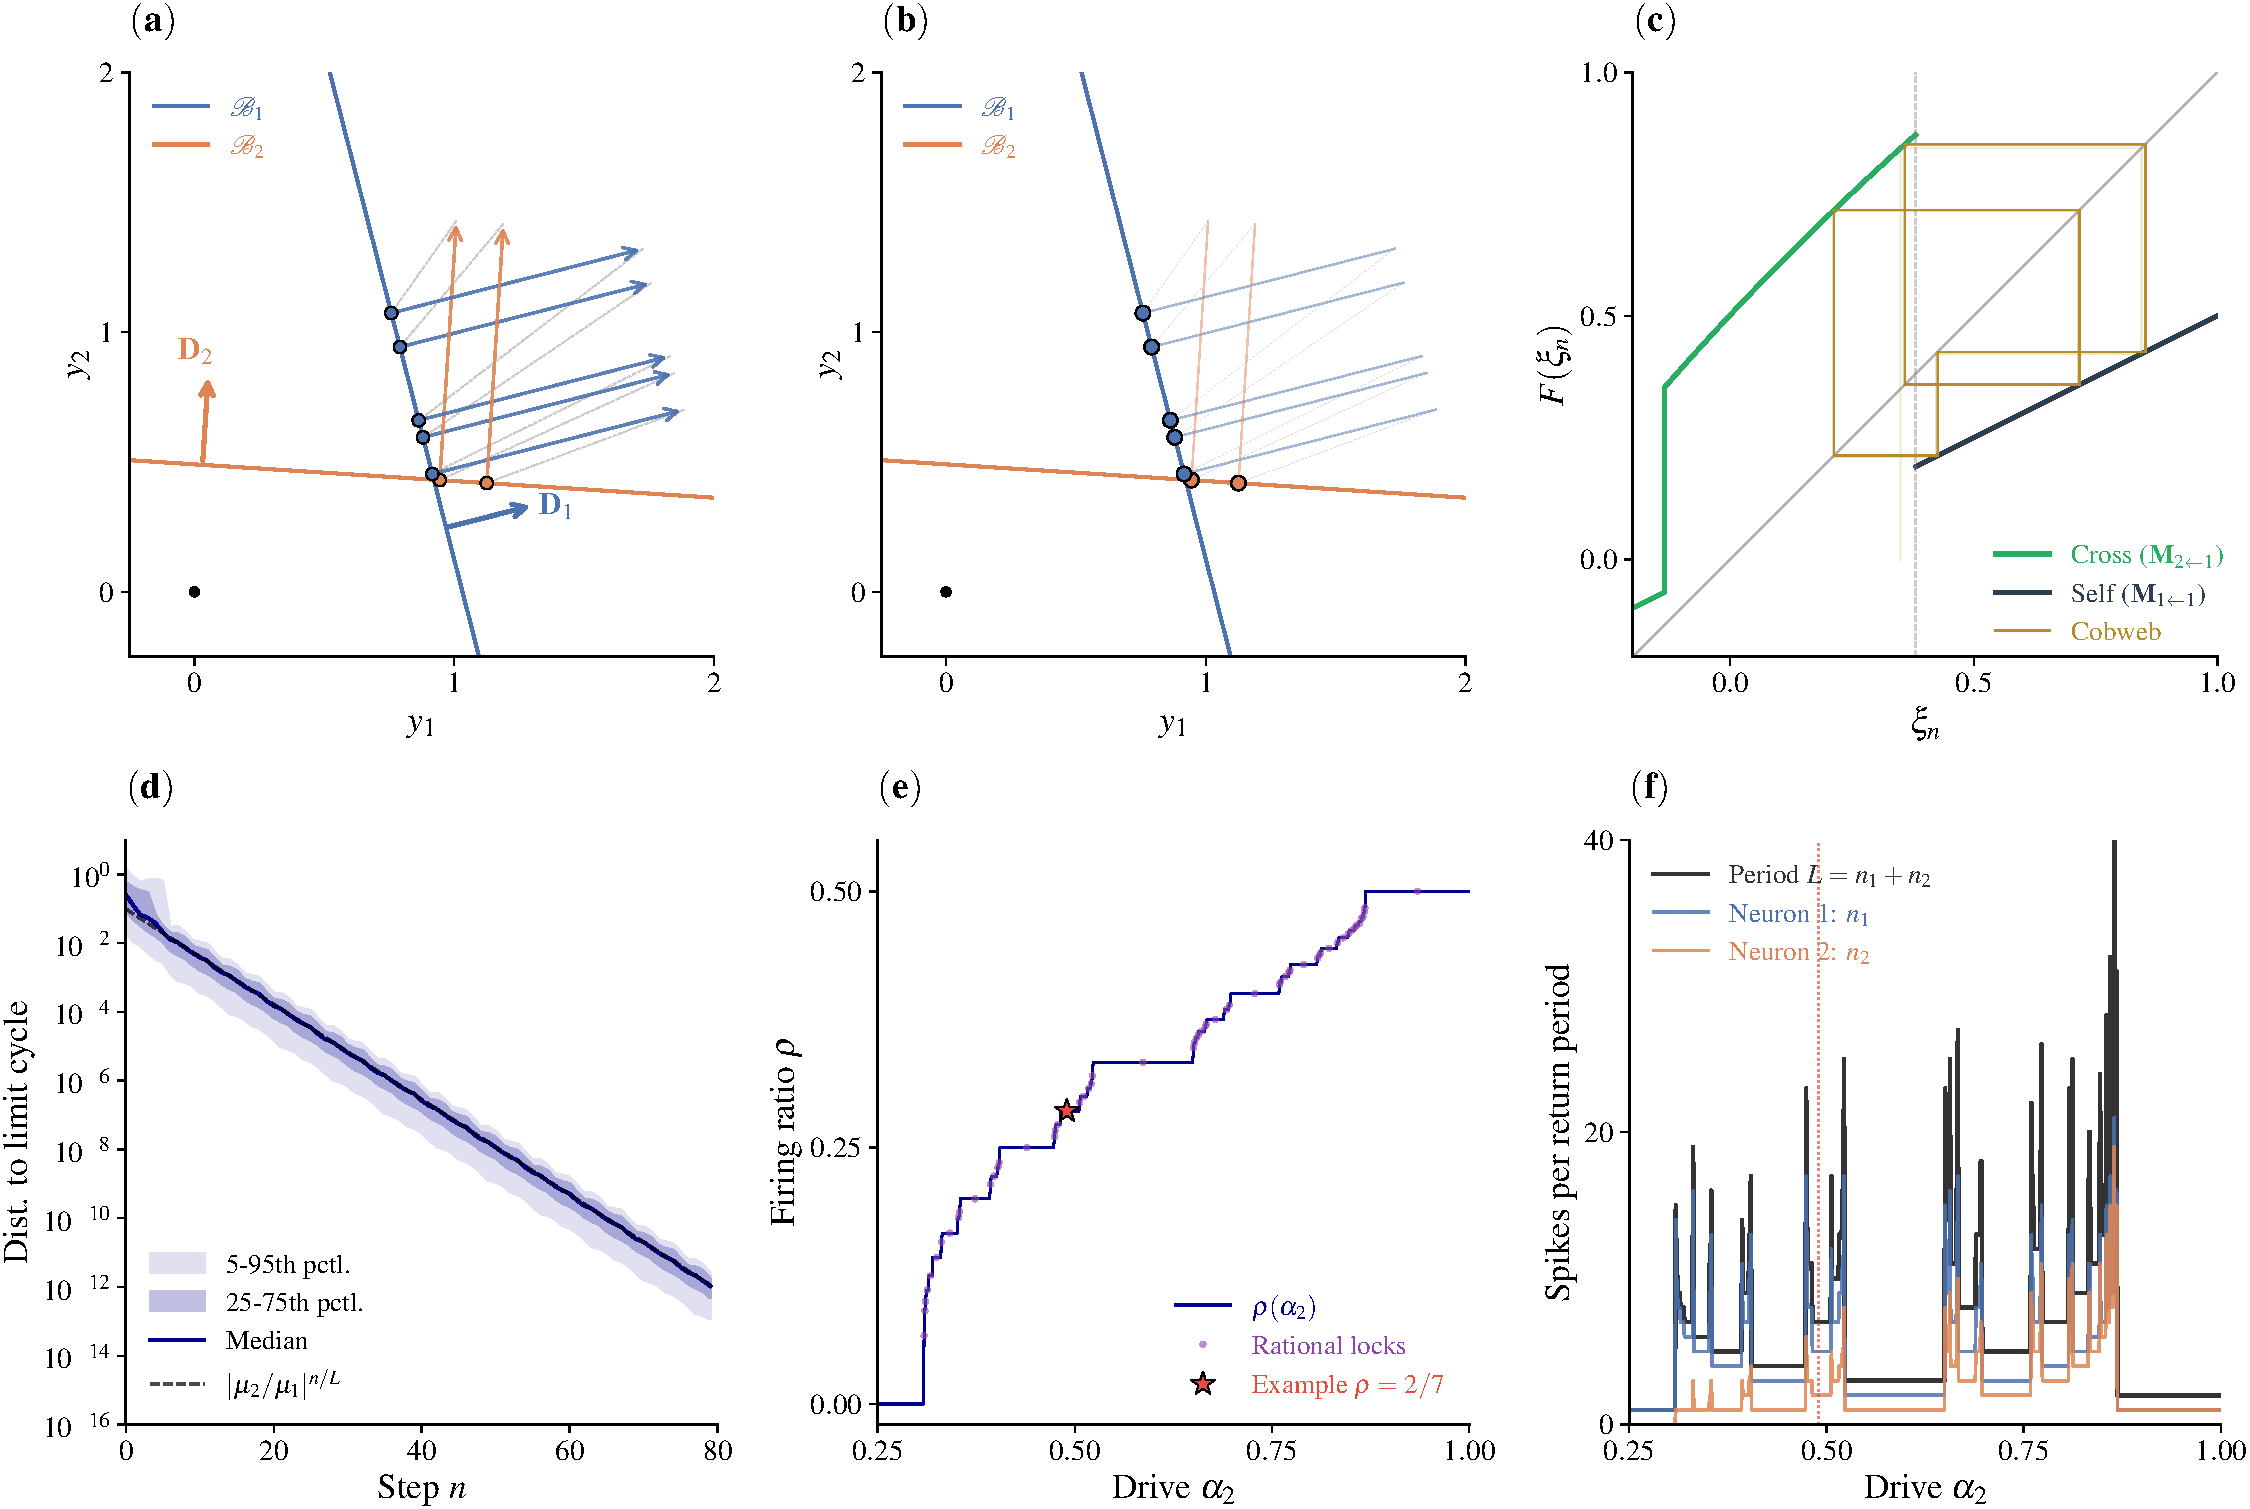
\includegraphics[width=\textwidth]{figures/scn_word_example.pdf}
\caption{Overview of SCN dynamics for $N=K=2$, $\psi=0.4\pi$, at the period-$7$ working point $\sigma=(1,1,2,1,1,1,2)$, $\alpha_1=1.0$, $\alpha_2=0.49$. \textbf{(a)}~Decoders, spike bounds, and one numerically simulated orbit period after convergence. \textbf{(b)}~The seven positions predicted by the dominant eigenvector of $\vv{M}_\sigma$ (Theorem~\ref{thm:eigvec}). \textbf{(c)}~Cobweb of the first-return map $F_{\!\Bsp_1}$: two M\"obius branches (blue self, red cross) meeting at $\xi_{\mathrm{part}}$; the amber cobweb converges to the period-$5$ cycle on $\Bsp_1$. \textbf{(d)}~Convergence from random initial conditions decays at the predicted rate $|\mu_2/\mu_1|^{n/L}$ (dashed). \textbf{(e)}~Devil's staircase (Theorem~\ref{thm:staircase}): firing ratio $\rho_{\mathrm{spike}}=k/(q+k)$ vs.\ $\alpha_2$ (see Remark~\ref{rem:rho-conventions}); star marks the panel~(a)--(c) operating point at $\rho_{\mathrm{spike}}=2/7$. \textbf{(f)}~Spike counts $n_1,n_2$ per return period as $\alpha_2$ varies; on each mode-locked plateau both counts are integer-constant, and only the plateau boundaries produce discontinuous jumps.}
\label{fig:overview}
\end{figure}

\subsection{Completeness of the staircase}\label{sec:completeness}
\begin{theorem}[Continuity, monotonicity, and surjectivity of the firing ratio]\label{thm:staircase}
For $K{=}N{=}2$ in $\RR^2$ with fixed $	heta_1\in\RR$, $\psi\in(0,\pi/2)$ (so $\cos\psi>0$), and $\alpha_1>0$, the firing ratio $\rho(\alpha_2)$ of the first-return map $F_{\!\Bsp_1;\alpha_2}:\Bsp_1\to\Bsp_1$ (distinct from the full-cycle map $F$ of Eq.~\eqref{eq:F-from-M}) satisfies, for $\alpha_2\in[\alpha_1\cos\psi,\,\alpha_1/\cos\psi)$ (the admissibility window in which both branches remain physical, cf.~\eqref{eq:margin}):
\begin{enumerate}[label=\textup{(\roman*)},leftmargin=*]
    \item $\alpha_2\mapsto\rho(\alpha_2)$ is continuous;
    \item $\alpha_2\mapsto\rho(\alpha_2)$ is monotone non-decreasing;
    \item $\rho(\alpha_1\cos\psi)=0$ and $\rho(\alpha_2)\to 1$ as $\alpha_2$ increases to $\alpha_1/\cos\psi$ from below, so every rational $p/q\in(0,1)$ is attained on a closed interval of positive Lebesgue measure (a mode-locked plateau) on which the orbit is a stable period-$q$ cycle; every irrational $\omega\in(0,1)$ is attained at a single $\alpha_2$.
\end{enumerate}
Beyond the admissibility window ($\alpha_2\geq\alpha_1/\cos\psi$), both the neuron-$1$ self-trap on $\Bsp_1$ (giving $\rho=0$) and a neuron-$2$ self-trap on $\Bsp_2$ (giving $\rho=1$) are locally stable; which one is realized depends on the initial condition. Generic initial conditions in the natural continuation of the neuron-$1$ basin still give $\rho=0$; the natural continuation of the interior $\rho\to 1$ limit corresponds to trajectories captured by the neuron-$2$ self-trap.
\end{theorem}

\begin{proof}[Proof sketch] Continuity follows from the Rhodes--Thompson extension of Poincar\'e's rotation-number theory to the class of degree-$1$ non-decreasing lifts \citep{rhodes1991topologies,herman1979conjugaison}. Monotonicity uses that increasing $\alpha_2$ makes the cross-branch predicate $c_2>c_1$ switch only from FALSE to TRUE at any fixed tangent coordinate, giving a lift-dominance argument on rotation numbers. Surjectivity follows by the intermediate-value theorem across the admissibility window plus the standard Arnold-tongue positive-measure result~\citep{arnold1961small} (Theorem~\ref{thm:supp:arnold-tongue}) at every rational rotation number. The full argument is in Appendix~\ref{app:staircase-proof} in the supplementary material.\end{proof}

\begin{corollary}[Symbolic rigidity within a plateau]\label{cor:within-plateau}
On the interior of the $\rho=p/q$ plateau of Theorem~\ref{thm:staircase}, every $\alpha_2$ realises the \emph{same} firing word, the mechanical Sturmian word $\sigma_{p/q}$ (Definition~\ref{def:supp:sturmian}; cf.\ Remark~\ref{rem:sturmian}), up to a cyclic shift fixed by the choice of starting orbit index. The geometric orbit positions $\xi_0^*(\alpha_2),\ldots,\xi_{q-1}^*(\alpha_2)$ vary real-analytically with $\alpha_2$, but the cyclic ordering of firings (the symbolic word) does not.
\end{corollary}

\begin{proof}[Proof sketch] On the plateau interior, $\rho$ is constant at $p/q$ and the orbit is a stable period-$q$ cycle; Sturmian uniqueness for $K=2$ \citep{coven1973sequences,lothaire2002algebraic} pins the word up to cyclic shift, and continuity of the admissibility margin $m(\alpha_2)$ throughout the plateau interior prevents symbolic changes. Full argument in Appendix~\ref{app:staircase-proof} in the supplementary material.\end{proof}

\begin{remark}[Irrational firing ratios and quasi-periodicity]\label{rem:irrational} Irrational firing ratios such as $\rho_F=1/\pi$ occur on the nowhere-dense complement of the union of rational plateaus. Under the piecewise-M\"obius regularity of Theorem~\ref{thm:cone} this complement is a Cantor set to which the ``complete devil's staircase'' picture of \citet{jensen1983complete} applies (see also \citealp{herman1979conjugaison}); the singular parameter $\alpha_2^*$ can be located to ${\sim}50$ digits by a Farey/continued-fraction cascade (Appendix~\ref{app-rem:irrational} and Appendix~\ref{app:pi-cascade}). \end{remark}

\begin{remark}[Connection to periodically driven oscillators]\label{rem:driven-oscillators} The staircase is analogous to mode-locking in periodically driven neural oscillators \citep{glass1988clocks}, but here $\alpha_2$ shapes the intrinsic geometry under constant input rather than a time-varying forcing, and the projective structure gives exact analytical control over each plateau (Appendix~\ref{app-rem:driven-oscillators}). \end{remark}

\begin{remark}[Sturmian structure of firing words]\label{rem:sturmian} For $K=2$ with $\cos\psi>0$, the realizable finite firing words are exactly the mechanical Sturmian sequences $\sigma_{p/q}$ (equivalently, the symbolic dynamics of a rigid rotation by $\rho$), and at an irrational $\omega$ the limit is a genuine aperiodic Sturmian word (Appendix~\ref{app-rem:sturmian}). \end{remark}

%\begin{remark}[Staircases under other parameter sweeps]\label{rem:other-staircases}
%Theorem~\ref{thm:staircase} singles out $\alpha_3$ because monotonicity is structural in that direction: $\partial c_3/\partial\alpha_3>0$ at fixed $\yy^+$ while $c_2$ is independent of $\alpha_3$. Sweeping a different parameter inside the cone-preserving regime $\cos\psi>0$ (i.e., $\psi\in(0,\pi/2)$), the inter-decoder angle $\psi$ itself, the first decoder angle $	heta_2$, or $\alpha_2$, still produces a circle-homeomorphism family that depends continuously on the parameter, so the rotation number is still continuous; mode-locked plateaus still appear at every rational; and within each plateau, Corollary~\ref{cor:within-plateau} still pins the firing word to a single Sturmian. What changes is whether the structural monotonicity argument transfers. For $\psi$, the relevant derivative at fixed $\yy^+$ is $\partial(\DD_3^\top\yy^+)/\partial\psi = \vv{E}_2^\top\yy^+$, a sinusoid in $\psi$ whose sign depends on the local geometry. For the parameter choice of Figure~\ref{fig:psi_staircase} (asymmetric drives $\alpha_2{=}1$, $\alpha_3{=}0.5$, $	heta_2{=}0.25$) this derivative is positive throughout the cone-preserving range $\psi\in(0,\pi/2)$, so $\rho(\psi)$ is monotone non-decreasing, but for other choices of $	heta_2$ or asymmetric drives the sign can flip within the cone-preserving range and produce a \emph{non-monotone} staircase. The IVT-based surjectivity argument of Theorem~\ref{thm:staircase}(iii) is therefore only guaranteed for the $\alpha_3$ sweep; for $\psi$ it must be checked case by case. At the boundary $\psi=\pi/2$ the cone-preservation breaks down, and for $\psi>\pi/2$ the dynamics enters the chaotic regime described by Theorem~\ref{thm:cone}, so the staircase analysis applies only on $(0,\pi/2)$. The story is therefore parameter-agnostic at the staircase-structure level within the cone-preserving regime, but monotonicity, and hence the surjectivity argument of Theorem~\ref{thm:staircase}(iii), is special to $\alpha_3$.
%\end{remark}
%
%\begin{figure}[!h]
%\centering
%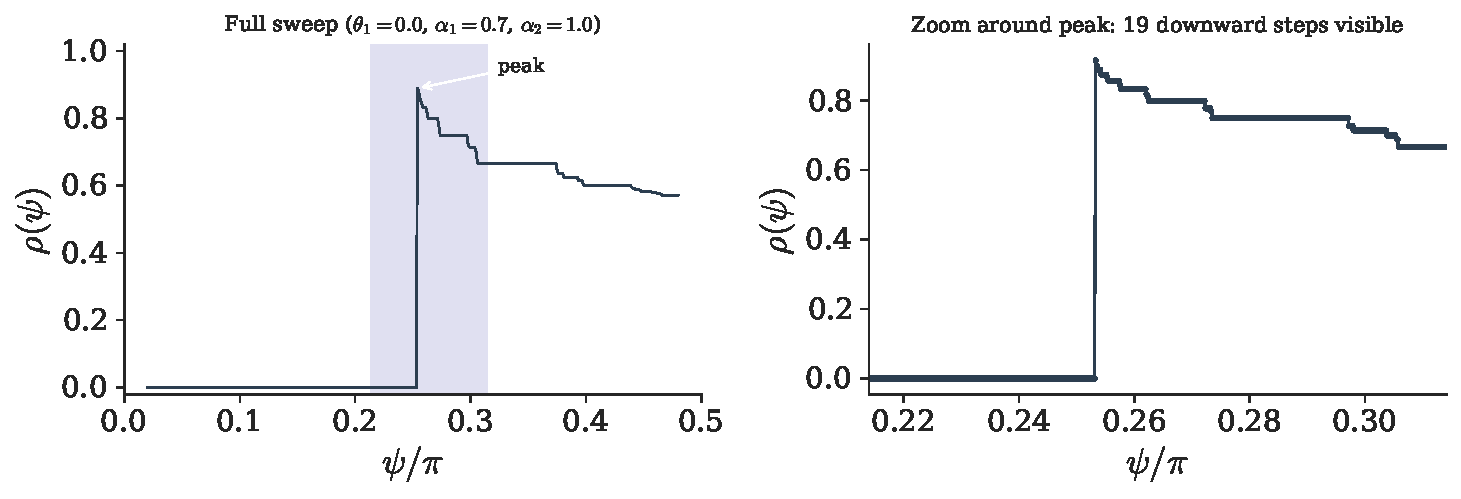
\includegraphics[width=0.95\textwidth]{figures/psi_staircase.pdf}
%\caption{Non-monotone devil's staircase under a $\psi$-sweep ($	heta_2{=}0$, $\alpha_2{=}0.7$, $\alpha_3{=}1.0$). \textbf{Left:} full sweep across the cone-preserving range $\psi\in(0.02\pi,\,0.48\pi)$; $\rho(\psi)$ climbs from $0$ to a local maximum near $\psi/\pi\approx 0.25$ and then descends, with $28$ downward steps of magnitude $>10^{-3}$ across the $400$-sample sweep. Shaded band: zoom window in the right panel. \textbf{Right:} dense zoom around the peak, individual sample markers shown; the staircase structure with multiple distinct downward step transitions is now resolvable. The non-monotonicity reflects that $\partial(\DD_3^\top\yy^+)/\partial\psi=\vv{E}_2^\top\yy^+$ can change sign across the orbit as $\psi$ varies, so the IVT-based surjectivity argument of Theorem~\ref{thm:staircase}(iii) does not automatically transfer to the $\psi$-sweep. The shape is parameter-specific: for other $(	heta_2,\alpha_2,\alpha_3)$ choices the $\psi$-staircase can be monotone.}
%\label{fig:psi_staircase}
%\end{figure}

\subsection{Realizable firing words}

The realizable-firing-word question has two dual aspects: \emph{existence} (for a target $\sigma$, do parameters $(\vv{D},\boldsymbol{\alpha})$ exist that realize it as a stable admissible orbit?) and \emph{universality} (does some SCN realize \emph{every} prescribed finite periodic word?). The $K{=}N{=}2$ classification proved below answers both for the binary case: existence holds if and only if $\sigma$ is a mechanical Sturmian sequence, and universality fails because non-Sturmian binary words are unrealizable. For $K\geq 3$ the partition geometry is far richer, the inverse-problem solver of Section~\ref{sec:inverse} produces stable admissible orbits for every word we have tested up to $K{=}6$, and universal-approximation theorems for dynamical systems with infinite-time-horizon guarantees~\citep{AnonSelfCite2026b} suggest that the SCN is universal in this regime: any prescribed finite periodic firing word should be realizable at sufficiently large $K,N$. We do not prove this conjecture but state it as Conjecture~\ref{conj:universality}.

\begin{conjecture}[Universality of SCN firing words for $K{\geq}3$]\label{conj:universality}
For every finite periodic firing word $\sigma=(b_0,\ldots,b_{L-1})$ over an alphabet $\{1,\ldots,K\}$ with $K\geq 3$ that uses each symbol at least once, there exist a network size $N\leq N_\star(K,L)$, decoders $\vv{D}\in\RR^{N\times K}$, and drives $\boldsymbol{\alpha}\in\RR_{>0}^{K}$ satisfying the cone-preserving condition $\cos\psi_{ij}>0$ for all $i,j$, such that the SCN with parameters $(\vv{D},\boldsymbol{\alpha})$ realizes $\sigma$ as a stable admissible periodic orbit. Here $N_\star(K,L)$ is a finite bound depending only on $K$ and $L$.

\emph{Empirical status.} The inverse solver of Section~\ref{sec:inverse} finds admissible cone-preserving parameters for every $\sigma$ tested up to $K=6$, $L=11$, all with $N\leq \max(K,L)$; the strongest bound consistent with the tested cases is $N_\star(K,L)\leq\max(K,L)$. Cone geometry additionally forces the lower bound $N_\star(K,L)\geq K-1$ when $L\geq K$: realising a word that uses every symbol requires the $K$ decoders $\DD_i$ to be pairwise linearly independent under the cone-preserving condition $\cos\psi_{ij}>0$, and $K$ such vectors fit in $\RR^N$ only when $N\geq K-1$. So the conjecture is only nontrivial when $L$ is large relative to $K$. Tested rows of Table~\ref{tab:highd} with $K_{\text{act}}<K$ (i.e., $\sigma$ using fewer than $K$ distinct symbols) do not directly witness the conjecture at the nominal alphabet size $K$; the strongest ``each-symbol-used'' evidence is the $(K=4,N=50)$ Simon network of Section~\ref{sec:apps-simon} and the $(K=5,N=50)$ multi-word entry of Table~\ref{tab:highd}, both realized by the same solver. The critical open stress test is whether the non-permutation, symbol-repeating word $(0,1,0,2)$ is realizable at $K=3$ for some $N$; if it is not, the conjecture as stated is falsified and the bound must depend on structural features of $\sigma$ beyond $(K,L)$.
\end{conjecture}

\subsubsection{From SCN dynamics to Sturmian words: $K{=}2$}\label{sec:sturmian-chain}

The structural results assembled so far, the projective reduction (Theorem~\ref{thm:projective}), the staircase theorem (Theorem~\ref{thm:staircase}), within-plateau rigidity (Corollary~\ref{cor:within-plateau}), and the Sturmian remark (Remark~\ref{rem:sturmian}; formal definition of Sturmian sequences: Definition~\ref{def:supp:sturmian}), combine into a sharp \emph{classification} of which binary firing words the $K{=}N{=}2$ SCN can realize. The statement is bidirectional: exactly the mechanical Sturmian sequences, and nothing else. We assemble the chain of reasoning here, both because it makes the structure of the family precise and because it puts the SCN into a classical combinatorial setting (Morse--Hedlund \citeyearpar{morse1938symbolic,morse1940symbolic}; Lothaire \citeyearpar{lothaire2002algebraic}).

The classification chain proceeds in four steps: circle-map reduction (Prop.~\ref{prop:circle-homeo}) $\to$ Poincar\'e rotation number (Thm.~\ref{thm:staircase}) $\to$ Diophantine conjugacy to $R_\rho$ \citep{liousse2005nombre,herman1979conjugaison} $\to$ Morse--Hedlund/Coven--Hedlund Sturmian encoding \citep{morse1938symbolic,coven1973sequences}, extended off single $\alpha_2$ to plateau interior by Cor.~\ref{cor:within-plateau}.
Appendix~\ref{app:sturmian-chain} in the supplementary material gives the argument in full.

\begin{theorem}[Classification of realizable $K{=}2$ firing words]\label{thm:classification}
For the $K{=}N{=}2$ SCN with $	heta_1\in\RR$, $\psi\in(0,\pi/2)$, $\alpha_1>0$, and $\alpha_2$ in the open admissibility window $(\alpha_1\cos\psi,\,\alpha_1/\cos\psi)$ (Theorem~\ref{thm:staircase}), the set of firing words realized by stable periodic orbits as $\alpha_2$ varies is exactly
\[
    \bigl\{\sigma_{p/q}\ :\ p/q\in(0,1)\cap\mathbb{Q},\ \gcd(p,q)=1\bigr\} \;\big/\; \text{cyclic shift},
\]
where $\sigma_{p/q}$ is the mechanical Sturmian. Each $\sigma_{p/q}$ is realized on the interior of a closed interval of $\alpha_2$ of positive Lebesgue measure (its plateau); on the plateau interior Corollary~\ref{cor:within-plateau} gives symbolic rigidity, and the closure is added by Sturmian uniqueness at the plateau endpoints. At the two endpoints of the admissibility window ($\alpha_2\in\{\alpha_1\cos\psi,\alpha_1/\cos\psi\}$) the map ceases to be a two-branch circle map: at the lower endpoint every step is a self-transition ($\rho=0$, constant word $\bar{0}$) and at the upper endpoint the neuron-$2$ self-trap becomes admissible ($\rho=1$, constant word $\bar{1}$); these two degenerate ``endpoint'' words fall outside the mechanical-Sturmian family and are the only realizable binary words in the closed regime $[\alpha_1\cos\psi,\alpha_1/\cos\psi]$ not of the form $\sigma_{p/q}$ with $p/q\in(0,1)$. Beyond the window, no new binary words are realized (both endpoint self-traps persist). No non-Sturmian binary word (in the aperiodic sense) is the firing word of any $K{=}N{=}2$ SCN at any $\alpha_2\in(\alpha_1\cos\psi,\alpha_1/\cos\psi)$.
\end{theorem}

\begin{proof}
The set of realized words is contained in the Sturmians by Steps 1--6 above. Each rational $p/q\in(0,1)$ is attained on a plateau of positive measure by Theorem~\ref{thm:staircase}(iii), and the firing word on that plateau is $\sigma_{p/q}$ by Step~7. Conversely, every Sturmian $\sigma_{p/q}$ for $p/q\in(0,1)$ arises this way, since its plateau is nonempty. No non-Sturmian word can be realized, because every realized word is forced to be a partition-encoding of a circle rotation, hence Sturmian.
\end{proof}

\subsubsection{$K>2$}

\begin{remark}[Why higher $K$ is qualitatively different]\label{rem:K-geq-3-richer} For $K\geq 3$ the $K$-cell partition escapes the Morse--Hedlund complexity rigidity \citep{morse1938symbolic,morse1940symbolic} and the three-distance theorem \citep{sos1957distribution,swierczkowski1958successive} that jointly pin the $K=2$ words to Sturmians, so the realizable-word class becomes much larger and we treat it heuristically via the inverse problem of Section~\ref{sec:inverse} (Appendix~\ref{app-rem:K-geq-3-richer}). \end{remark}

\begin{conjecture}[Sofic structure of realized words for cone SCNs, $K\geq 3$]\label{conj:sofic}
Fix cone-preserving parameters $(\{\DD_i\}_{i=1}^K, \{\alpha_i\}_{i=1}^K)$ with $\cos\psi_{ij}>0$ for all $i,j$ and drives $\alpha_i\in[\alpha_{\min},\alpha_{\max}]\subset(0,\infty)$. Let $X_{\vv{D},\boldsymbol{\alpha}}\subset\{1,\ldots,K\}^{\mathbb{Z}}$ be the shift-closure of the periodic bi-infinite firing sequences of stable admissible orbits of the SCN at these parameters. Then $X_{\vv{D},\boldsymbol{\alpha}}$ is a \emph{sofic shift}: a shift space whose admissible bi-infinite sequences are the labels of bi-infinite paths through some finite directed graph (equivalently, a factor of a \emph{subshift of finite type}, in which the admissible blocks are characterized by a finite list of forbidden patterns) \citep{lind2021introduction}.
\end{conjecture}

The conjecture is motivated by two structural facts: Birkhoff--Hilbert contraction (Theorem~\ref{thm:cone}(a), formal statement Theorem~\ref{thm:supp:birkhoff-hilbert}) shrinks the effect of the past exponentially, and the next-firer partition has bounded margin at generic parameters, so at most $K$ follower sets are needed after long enough pasts (a stronger property than sofic). A precise proof would go through a Markov-partition construction for piecewise projective contractions and Krieger's factor-map theorem for subshifts of finite type \citep{lind2021introduction}. See Appendix~\ref{app:sofic-heur} in the supplementary material.
\subsection{Higher-dimensional examples}\label{sec:highd}

The eigenvector construction is exact for any $(K,N)$. A representative $K=3$, $N=3$ system with symmetric all-inhibitory decoders (pairwise $\cos\psi_{ij}=0.507$) and drives $\boldsymbol{\alpha}=(1.0,0.9,0.7)$ produces the period-$11$ word $\sigma=(2,1,3,2,1,2,1,3,1,2,1)$ with firing ratios $(5/11,4/11,2/11)$: the $3\times 3$ return-map eigenvector predicts all $11$ orbit points exactly, and both stability ratios ($|\mu_2/\mu_1|=0.015$, $|\mu_3/\mu_1|=0.008$) are well inside the unit circle. Three new features distinguish $K\geq 3$ from $K=2$: $N-1$ eigenvalue ratios to check rather than one (Theorem~\ref{thm:eigvec}); partition boundaries on each bound are affine hyperplanes rather than points; and multistability between the mixed cyclic orbit and self-trapping single-bound orbits becomes possible. Full details are in Appendix~\ref{app:3d-example}. A systematic verification on $13$ random configurations spanning square ($K=N$), underdetermined ($K<N$), and overdetermined ($K>N$) regimes agrees with Theorem~\ref{thm:eigvec} to machine precision ($\|\text{err}\|_\infty<10^{-14}$) in every case; the configurations, firing words, and Table~\ref{tab:highd} are in Appendix~\ref{app:highd-verif}.

\subsection{Chaos with opposing decoders}\label{sec:chaos}

The absence of chaos depends critically on the decoder geometry. When all pairwise cosines $\cos\psi_{ji}>0$, every pair of decoders forms an acute angle and the decoders therefore all lie in a common open half-space of~$\RR^N$. More precisely, the post-spike readout $\yy^+=(\alpha_i+1)\DD_i+\vv{U}_i\xxi$ has all components of $\DD_j^\top\yy^+>0$ when $\cos\psi_{ji}>0$, so the decay ray stays in the open ``positive cone'' $\mathcal{C}=\{\yy:\DD_j^\top\yy>0\;\forall j\}$ defined by the decoders. A classical result of Birkhoff guarantees that any linear map preserving such a cone contracts a natural projective notion of distance on it (the \emph{Hilbert metric}), with contraction ratio bounded by $\tanh(\Delta/4)$ where $\Delta$ is the projective diameter of the image cone. Since consecutive images are bounded (the spike adds a fixed vector $\DD_i$), the contraction is uniform, ruling out positive Lyapunov exponents. This result is consistent with the findings of \citet{jahnke2008stable} and \citet{jahnke2009chaotic}, who showed that purely inhibitory pulse-coupled networks exhibit ``stable irregular dynamics'' that converges to periodic orbits \citep[see also][]{jin2002fast}, despite appearing chaotic at short timescales. Our Hilbert metric argument provides the geometric mechanism underlying their numerical observations.

When at least one $\cos\psi_{ji}<0$, the post-spike readout can leave the cone (some $\DD_j^\top\yy^+$ becomes negative), and the projective map may pull nearby states apart instead of pushing them together. Chaos in spiking networks with mixed excitatory-inhibitory connectivity was first demonstrated by \citet{vreeswijk1996chaos} in large balanced networks; our framework provides an exact geometric characterization of this transition for small structured networks. A systematic scan of 800 random (decoder, drive) combinations for $K=4$, $N=3$ (Figure~\ref{fig:chaos}a) confirms the sharp dichotomy: zero chaotic cases among positive-cosine samples, versus 5 chaotic cases ($\lambda_{\max}>0$) among negative-cosine samples. The Lyapunov exponents range from $\lambda_{\max}\approx 0.004$ (weakly chaotic, visible as the red star nearest $\lambda_{\max}=0$ in Figure~\ref{fig:chaos}a) to $\lambda_{\max}\approx 0.21$, indicating that the onset of chaos is continuous rather than an abrupt transition.

We verify one chaotic case rigorously ($\cos\psi_{\min}=-0.57$). The trajectory is aperiodic (no period up to 8000), all four neurons fire (at rates 19\%, 24\%, 41\%, 17\%), and the block entropy grows steadily ($H=1.91,\,3.02,\,3.72,\,4.27,\,4.78$ bits for block lengths $L=1,\ldots,5$). Trajectories starting $\varepsilon=10^{-12}$ apart diverge in their firing words after ${\sim}90$ steps, scaling as $\Delta t\propto\ln(1/\varepsilon)/\lambda_{\max}$ (Figure~\ref{fig:chaos}b). The attractor projected onto the tangent space of the most-visited bound shows fractal structure (Figure~\ref{fig:chaos}c).

Because the transition map~\eqref{eq:transition-map} is a known rational function of $\xxi$, the $2\times 2$ Jacobian can be computed exactly at each step (Appendix~\ref{app:numerics}). QR-based accumulation over 50 independent segments of 1000 steps gives $\lambda_1=0.285\pm 0.010$, with all segments positive ($2\sigma$ lower bound $0.265$). The chaos mechanism is heterogeneous: some transitions always expand (e.g.\ $0\to 1$, min singular value $3.25$), others always contract ($1\to 0$, max $0.62$), and the net expansion is positive. Strikingly, every short periodic sub-word extracted from the chaotic trajectory has a return map whose dominant eigenvector is mathematically \emph{stable} ($|\mu_2/\mu_1|<1$), yet none are admissible: the partition prevents the trajectory from settling into any periodic orbit \citep{korn2003there,terada2024chaotic}. The chaos is driven not by eigenvalue instability but by the piecewise structure itself.

\begin{figure}[t]
\centering
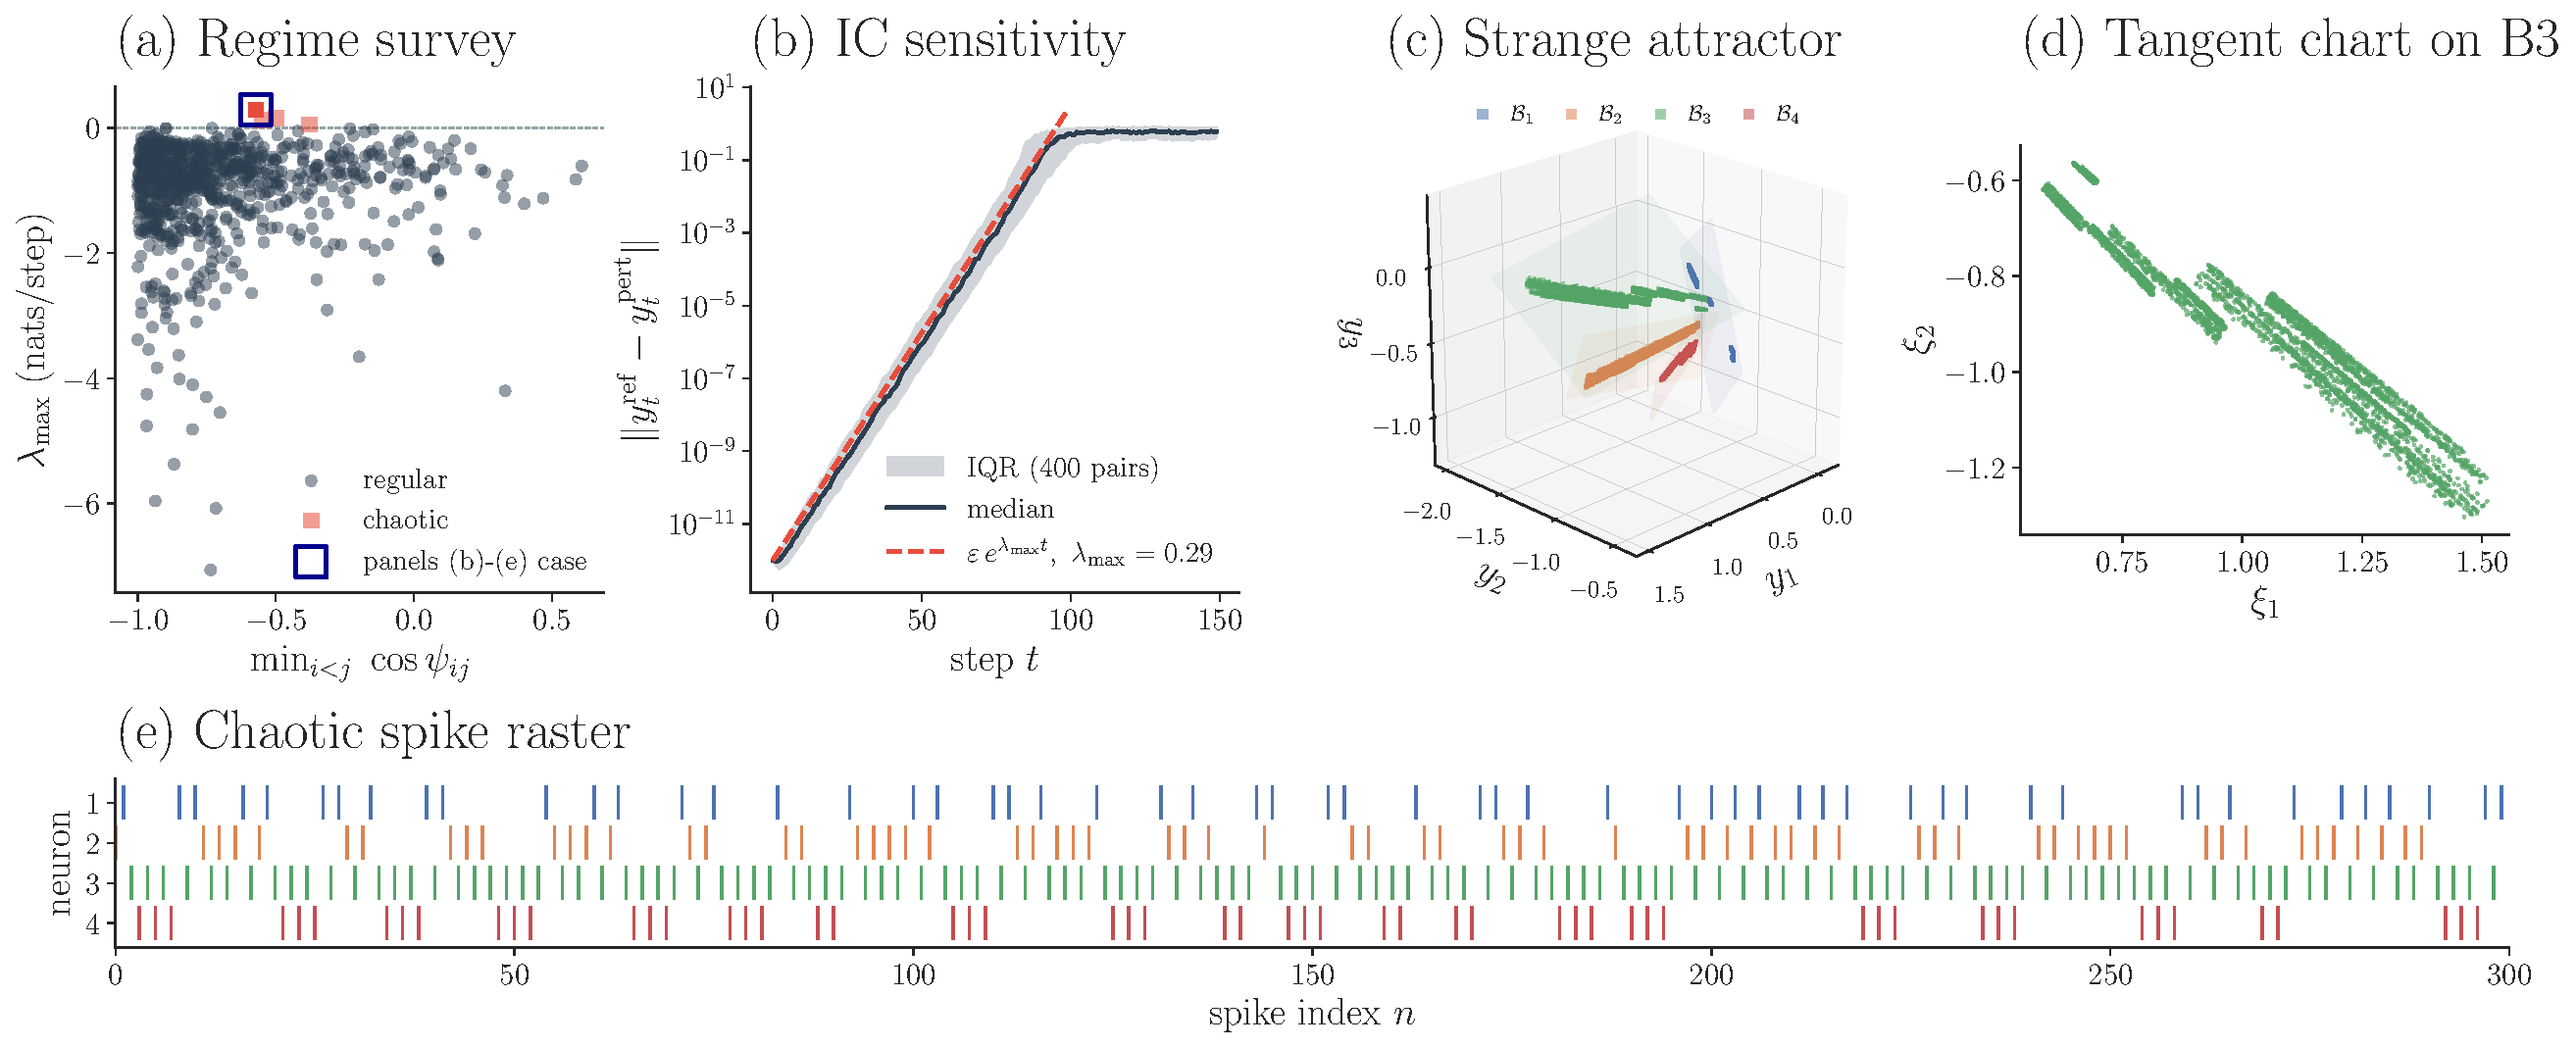
\includegraphics[width=\textwidth]{figures/chaos_figure.pdf}
\caption{Order--chaos transition ($K=4$, $N=3$). \textbf{(a)}~Phase diagram: $\lambda_{\max}$ vs.\ $\min_{i<j}\cos\psi_{ij}$ over 800 random samples; regular cases (dots) sit at $\lambda_{\max}\leq 0$, chaotic cases (squares) at $\lambda_{\max}>0$, all with negative minimum cosine. The accent-blue open square outlines the specific $(\vv{D},\boldsymbol{\alpha})$ case zoomed into panels (b), (c), (d). \textbf{(b)}~Sensitivity to initial conditions at $\cos\psi_{\min}=-0.57$: median distance of 400 trajectory pairs anchored at successive points along the converged orbit and each perturbed by $\varepsilon=10^{-12}$; the median grows as $e^{\lambda_{\max} t}$ with $\lambda_{\max}\approx 0.29$ (dashed, QR-measured), IQR shaded. \textbf{(c)}~Strange attractor on $\Bsp_3$ (${\sim}20\,000$ iterates in the tangent chart) for the panel~(b) case. \textbf{(d)}~Firing-neuron raster for the first 300 spikes of the same trajectory: the sequence never repeats, illustrating the aperiodicity underlying $\lambda_{\max}>0$.}
\label{fig:chaos}
\end{figure}

The boundary between order and chaos is thus the \emph{sign of the pairwise decoder cosines}: the cone geometry that enables sequence memory (Section~\ref{sec:inverse-applications}) is precisely the geometry that prevents chaos. We summarize this as the following dichotomy.

\begin{theorem}[Cone dichotomy: order vs.\ chaos]\label{thm:cone}
Let $\mathcal{C}=\{\yy\in\RR^N:\DD_i^\top\yy>0\text{ for all }i\}$ be the open positive cone of the SCN's decoders.
\begin{enumerate}[label=(\alph*)]
\item \emph{(Positive cosines $\Rightarrow$ order.)} If $\cos\psi_{ij}>0$ for every pair $(i,j)$, then every transition $\vv{M}_{j\leftarrow i}$ maps $\mathcal{C}$ into itself, and the projective map restricted to $\mathcal{C}$ strictly contracts the Hilbert projective metric on $\mathcal{C}$ with contraction ratio bounded uniformly away from~1 \citep{birkhoff1957extensions,bushell1973hilbert}. Consequently every admissible periodic orbit has $|\mu_k/\mu_1|<1$ for all $k\geq 2$ (Theorem~\ref{thm:eigvec}), and the maximal Lyapunov exponent of any trajectory is non-positive.
\item \emph{(Negative cosine permits chaos.)} If $\cos\psi_{ij}<0$ for some pair $(i,j)$, the cone $\mathcal{C}$ is no longer invariant. There exists at least one explicit choice of SCN parameters $(\DD,\boldsymbol{\alpha})$ with $\cos\psi_{\min}<0$ for which the maximal Lyapunov exponent $\lambda_{\max}=\lim_{n\to\infty}\frac{1}{n}\ln\sigma_1(n)$ along a generic trajectory is strictly positive and the dynamics is chaotic, where $\sigma_1(n)$ is the leading singular value of the $n$-step Jacobian; we construct one such instance below ($K=4$, $N=3$, $\cos\psi_{\min}=-0.57$). The frequency of chaotic versus stable behaviour across the negative-cosine regime is a separate empirical question; a scan of $800$ random $(K{=}4, N{=}3)$ parameter samples (Figure~\ref{fig:chaos}a) found 5 strictly chaotic cases, all with $\cos\psi_{\min}<0$.
\end{enumerate}
\end{theorem}
\begin{proof}[Proof sketch] See Appendix~\ref{app:chaos-details} in the supplementary material. Part~(a) is a Birkhoff--Hilbert contraction argument on the positive cone. Part~(b) exhibits an SCN with $K=4$, $N=3$ decoders (minimal pairwise cosine $\cos\psi_{\min}\approx-0.57$) whose per-step Jacobian, accumulated via QR over $50$ segments of $10^3$ steps, gives $\lambda_1=0.285\pm 0.010$ nats, with sensitivity to initial conditions and a fractal attractor cross-section confirming chaos.\end{proof}

See Appendix~\ref{app:chaos-details} in the supplementary material for the relation to \citet{vreeswijk1996chaos} balanced-network chaos and for the observation that the eigenvector machinery of Theorem~\ref{thm:eigvec} transfers verbatim across the cone boundary but with a different dynamical reading.

\begin{remark}[Quasi-periodic orbits are not chaotic]\label{rem:quasi-vs-chaos} At irrational firing ratios the orbit is quasi-periodic with maximal Lyapunov exponent zero (Proposition~\ref{prop:quasi-LE}), whereas genuine chaos requires at least one $\cos\psi_{ij}<0$ to break the cone (Appendix~\ref{app-rem:quasi-vs-chaos}). \end{remark}


%======================================================================
\section{The inverse problem: from prescribed firing word to network parameters}\label{sec:inverse}
%======================================================================

We now turn to the question that motivates much of this analysis: \emph{given a desired periodic firing word $\sigma=(b_0,\ldots,b_{L-1})$, can we find an SCN that produces it?} A positive answer would mean that any temporal sequence can be stored as a stable limit cycle in a recurrent spiking network, providing a model of \textbf{sequence working memory}.

\subsection{Problem statement}\label{sec:inverse-statement}

Fix decoders $\{\DD_i\}_{i=1}^{K}\subset\RR^N$ (unit vectors) and a target firing word $\sigma=(b_0,\ldots,b_{L-1})$. We seek drives $\boldsymbol{\alpha}\in\RR_{>0}^K$ such that $\sigma$ is realized as a stable admissible orbit of the SCN. Equivalently (Theorem~\ref{thm:eigvec}, Section~\ref{sec:partition}), the drives must satisfy three conditions:
\begin{enumerate}[label=(\roman*),nosep]
\item \emph{Existence.} The return map $\vv{M}_\sigma(\boldsymbol{\alpha})$ has a real eigenvector $\tilde\xxi^*=(\xxi^{*\top},1)^\top$ with $u_N\neq 0$.
\item \emph{Stability.} $|\mu_k(\boldsymbol{\alpha})/\mu_1(\boldsymbol{\alpha})|<1$ for every $k\geq 2$.
\item \emph{Admissibility.} At every step $k=0,\ldots,L-1$ of the eigenvector orbit, the first bound reached after a spike of neuron~$b_k$ is bound~$b_{k+1}$ (and not some other competitor).
\end{enumerate}
Conditions (i)--(ii) are eigenvalue conditions on $\vv{M}_\sigma(\boldsymbol{\alpha})$; condition (iii) is a polynomial inequality system. To make (iii) tractable for gradient-based search, we recast it as a continuous \textbf{admissibility margin} whose positivity is equivalent to the prescribed word being realized:
\begin{equation}\label{eq:margin}
    m(\boldsymbol{\alpha}) \;=\; \min_{k\in\{0,\ldots,L-1\}}\Bigl(\,c_{b_{k+1},k}(\boldsymbol{\alpha}) \;-\; \max_{j\neq b_{k+1}} c_{j,k}(\boldsymbol{\alpha})\,\Bigr),\qquad
    c_{j,k}(\boldsymbol{\alpha}) \;=\; \frac{\alpha_j}{\DD_j^\top\,\yy_k^+(\boldsymbol{\alpha})},
\end{equation}
where $\yy_k^+$ is the $k$-th post-spike readout evaluated at the eigenvector orbit of $\vv{M}_\sigma(\boldsymbol{\alpha})$. Each summand is the gap between the winning decay factor $c_{b_{k+1},k}$ and the largest competitor; $m(\boldsymbol{\alpha})>0$ at every step is equivalent to (iii). The inverse problem is then the smooth optimization
\begin{equation}\label{eq:invopt}
    \;\boldsymbol{\alpha}^*\;=\;\arg\max_{\boldsymbol{\alpha}\,\in\,\RR_{>0}^K}\;m(\boldsymbol{\alpha})\quad\text{subject to (i)--(ii)},\;
\end{equation}
maximized rather than merely made positive to obtain the most noise-robust realization (Section~\ref{sec:inverse-applications}). A target word $\sigma$ is \emph{feasible} iff there exists $\boldsymbol{\alpha}\in\RR_{>0}^K$ with $m(\boldsymbol{\alpha})>0$ and (i)--(ii) holding; in that case the feasible set
\begin{equation}\label{eq:admissible-set}
    \mathcal{A}_\sigma = \bigl\{\boldsymbol{\alpha}\in\RR_{>0}^K\,:\,(\text{i}),(\text{ii}),(\text{iii})\text{ hold}\bigr\}
\end{equation}
is nonempty.

\subsection{Semi-algebraic structure}

The constraints (i)--(iii) are polynomial in the drives: $\vv{M}_\sigma(\boldsymbol{\alpha})$ has entries polynomial in $\boldsymbol{\alpha}$ (from~\eqref{eq:return}), its dominant eigenvector $\xxi^*$ is an algebraic function of $\boldsymbol{\alpha}$, and the admissibility conditions~\eqref{eq:partition} are polynomial inequalities. The feasible set~\eqref{eq:admissible-set} is therefore a \textbf{semi-algebraic set}. Not all words are realizable for a given decoder geometry:

\begin{remark}[Word impossibility from decoder alignment]\label{rem:impossible} Two neurons with $\cos\psi_{ji}\approx 1$ cannot fire consecutively, since the large projection makes bound~$j$ reached last rather than first (Appendix~\ref{app-rem:impossible}). \end{remark}


\subsection{Analytical solution for $K=2$}

For two neurons in $\RR^2$, the realizable words are exactly the \emph{Sturmian} (balanced) sequences \citep{lothaire2002algebraic}: for any two subwords of the same length, the neuron-1 count differs by at most~1. Each word has rotation number $\rho=p/q$, and $\rho(\alpha_2)$ traces the devil's staircase (Figure~\ref{fig:overview}e). See Remark~\ref{rem:sturmian} for the symbolic-dynamics origin of this characterization.


\subsection{Exact recovery and the orbit--decoder identity}


For a \emph{permutation word} $\sigma=(b_0,\ldots,b_{K-1})$ in which each neuron fires exactly once per cycle ($L=K$), a prescribed orbit $(\yy_0,\ldots,\yy_{K-1})$ on the bounds uniquely determines both the decoders and the drives. The construction is geometric: between consecutive orbit points, the readout decays along the ray $\yy(\tau)=e^{-\lambda\tau}\yy_k^+$ toward the origin, so the post-spike readout $\yy_k^+=\yy_k+\DD_{b_k}$ must be collinear with $\yy_{k+1}$ through the origin. This gives the \textbf{orbit--decoder identity}: there exists $\lambda_k>0$ such that
\begin{equation}\label{eq:orbit-decoder}
    \;\DD_{b_k} \;=\; \lambda_k\,\yy_{k+1} \;-\; \yy_k,\qquad
        \lambda_k\text{ uniquely determined by }\|\DD_{b_k}\|=1.\;
\end{equation}
The unit-norm constraint fixes $\lambda_k$ as the positive root of the quadratic
$\lambda_k^2\|\yy_{k+1}\|^2 - 2\lambda_k\,\yy_k^\top\yy_{k+1} + \|\yy_k\|^2 - 1 = 0$,
and the drive $\alpha_{b_k}=\DD_{b_k}^\top\yy_k$ is then read off from the threshold condition~\eqref{eq:bound}. Each step thus recovers one decoder and one drive in closed form from the next orbit point, and the full network $(\vv{D},\boldsymbol{\alpha})$ is determined by the prescribed orbit up to a global rotation/reflection.


For non-permutation words ($L>K$, some neurons fire repeatedly), multiple orbit points lie on the same bound and \eqref{eq:orbit-decoder} is over-determined by a single transition: the decoders must be consistent across all visits to a bound. Multiplying the transition map~\eqref{eq:transition-map} through by its denominator yields, at each step $k$,
\begin{equation}\label{eq:bilinear}
    \bigl[(\alpha_{b_k}+1)\cos\psi_{b_{k+1}b_k} + \vv{v}_{b_{k+1}b_k}^\top\xxi_k\bigr]\,\xxi_{k+1}
    \;=\; \alpha_{b_{k+1}}\,\bigl[(\alpha_{b_k}+1)\,\vv{w}_{b_{k+1}b_k} + \vv{R}_{b_{k+1}b_k}\,\xxi_k\bigr],
\end{equation}
which is $N{-}1$ scalar equations bilinear in the drive pair $(\alpha_{b_k},\alpha_{b_{k+1}})$ when the orbit $(\xxi_k,\xxi_{k+1})$ and the decoder geometry are known. The $L$ transitions together give $L(N{-}1)$ bilinear equations in $K$ unknowns; with $L\geq K$ (which holds for any non-trivial word), the system is overdetermined and solved by least squares. Self-transitions ($b_{k+1}=b_k$) simplify to the explicit form $\alpha_{b_k}=(\xxi_{k+1}\!\cdot\!\xxi_k)/\|\xxi_k-\xxi_{k+1}\|^2$, reducing the unknown count further. We solve the full system~\eqref{eq:bilinear} numerically with SciPy's Levenberg--Marquardt root finder (Appendix~\ref{app:numerics}).

 Solving~\eqref{eq:invopt} by differential evolution (global) followed by Nelder--Mead (local), we find admissible drives for all tested words with $K\leq 3$ in $N=3$. In every case, the optimizer navigates the smooth margin landscape to find stable network parameters:

\begin{center}
\begin{tabular}{lccccl}
\hline
Word $\sigma$ & $L$ & $K$ & Margin & Stable & $\boldsymbol{\alpha}$\\
\hline
$(0,1)$ & 2 & 2 & 0.108 & yes & $(0.52,\;0.52)$\\
$(0,0,1)$ & 3 & 2 & 0.054 & yes & $(1.03,\;0.71)$\\
$(0,1,2)$ & 3 & 3 & 0.041 & yes & $(0.87,\;0.87,\;0.87)$\\
$(0,1,0,2)$ & 4 & 3 & 0.049 & yes & $(0.77,\;0.62,\;0.62)$\\
$(0,1,2,0,1)$ & 5 & 3 & 0.025 & yes & $(1.43,\;1.47,\;1.25)$\\
\hline
\end{tabular}
\end{center}


For permutation words $\sigma=(0,1,\ldots,K-1)$ on simplex decoders (pairwise cosine $\cos\psi_{ij}=(K\cdot 0.8^2-1)/(K\cdot 0.8^2+K-1)$, growing from $0.44$ at $K=2$ toward~$1$), the solver succeeds up to $K=6$ with monotonically shrinking margins (Figure~\ref{fig:inverse}d). At $K=7$--$8$ the pairwise cosine exceeds $\approx 0.83$ and the partition regions become too narrow: no $\boldsymbol{\alpha}\in\RR_{>0}^K$ satisfies $m(\boldsymbol{\alpha})>0$. The solver runs in ${\sim}0.2$\,s at $K=2$ and ${\sim}11$\,s at $K=6$, with empirical scaling close to $O(K^2)$.

\begin{figure}[H]
\centering
\begin{minipage}[c]{0.65\textwidth}
  \centering
  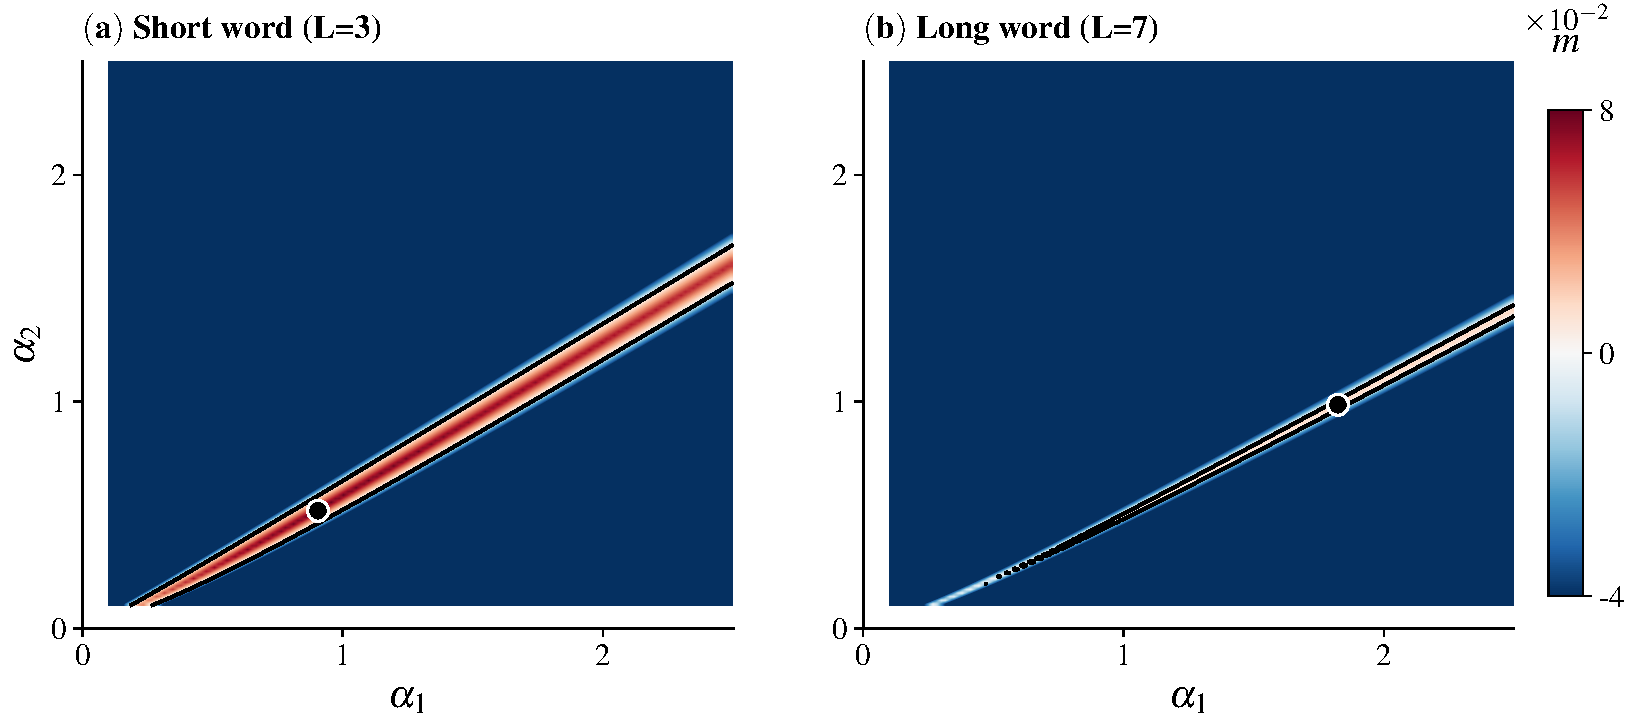
\includegraphics[width=\textwidth]{figures/margin_landscape.pdf}
\end{minipage}\hfill
\begin{minipage}[c]{0.33\textwidth}
  \centering
  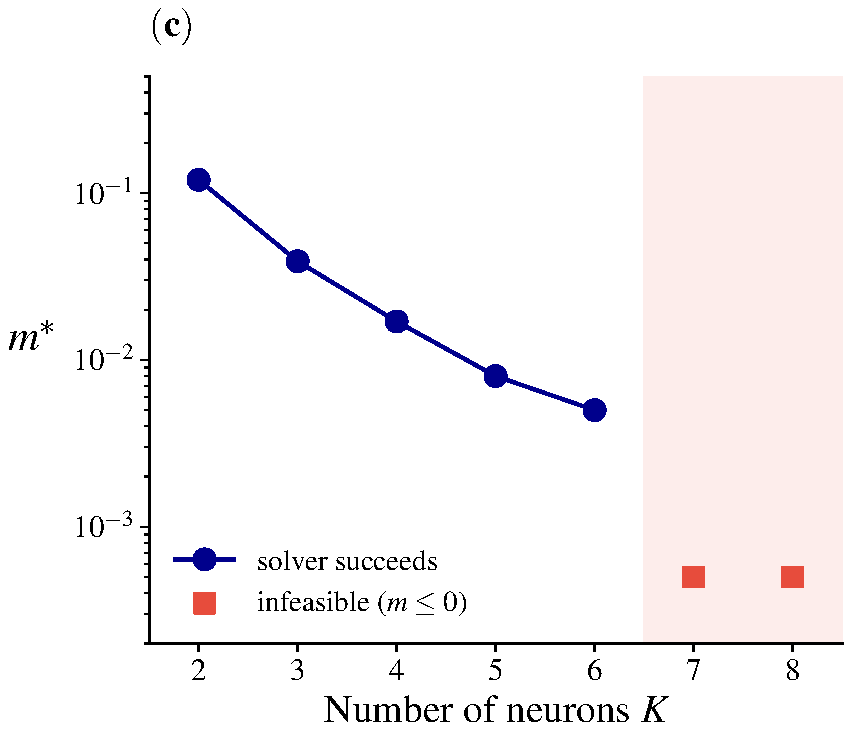
\includegraphics[width=\textwidth]{figures/inverse_scaling.pdf}
\end{minipage}
\caption{Inverse problem: margin landscape and solver scaling.
\textbf{(a),(b)}~Margin $m(\alpha_1,\alpha_2)$ for two target words ($K{=}N{=}2$, $\psi=0.4\pi$); the shared diverging colorbar (right) is centered on $m{=}0$: red $m>0$ (realized), blue $m<0$, black contour marks $m=0$. Circles locate the maximum-margin drives.
\textbf{(a)}~$\sigma=(1,1,2)$, $m_{\max}=0.08$, admissible at $\alpha_1>\alpha_2$.
\textbf{(b)}~$\sigma=(1,1,2,1,1,1,2)$: period-7 working point, thin sliver ($m_{\max}=0.02$); longer words shrink tolerances.
\textbf{(c)}~Simplex-decoder ($K=N$) permutation-word scaling: $m^*$ vs.\ $K$ (log). Red region ($K\geq 7$): pairwise cosine ${\gtrsim}0.83$ leaves no admissible drives. Margin shrinks geometrically with $K$, matching the $4\pm 1$ WM capacity (\S\ref{sec:inverse-applications}).}
\label{fig:inverse}
\end{figure}


Figure~\ref{fig:inverse}c fixes the decoder geometry to simplex configuration and optimizes over drives $\boldsymbol{\alpha}$ alone, which isolates the drive sub-problem for a clean cross-$K$ comparison. Relaxing the decoder constraint adds $K(N-1)$ free parameters and breaks the simplex's tight pairwise-cosine geometry that drives infeasibility at $K\geq 7$; joint $(\vv{D},\boldsymbol{\alpha})$ optimization is already used for the continuous-attractor construction in \S\ref{sec:inverse-applications}, and we expect it to extend the feasibility boundary substantially while preserving Dale's-law compliance through the cone constraint $\cos\psi_{ij}>0$ of Theorem~\ref{thm:cone}. The geometric limit is unavoidable in the all-inhibitory regime, however: as $K$ grows the inhibitory cone narrows, and very large $K$ ultimately requires growing $N$ too. Quantifying how much joint optimization gains across $K$ is a natural extension we have not pursued here.


The inverse problem stated above realizes one target word at a time. The \emph{multistability} that supports working memory in \S\ref{sec:inverse-applications} (the same $(\vv{D},\boldsymbol{\alpha})$ hosting many coexisting stable limit cycles, with input or initial condition selecting which one is realized) implicitly requires a stronger property: that the parameters realize all words in some prescribed set $\{\sigma^{(1)},\ldots,\sigma^{(m)}\}$ simultaneously. The natural multi-word formulation is
\begin{equation}\label{eq:multi-inverse}
    \max_{(\vv{D},\boldsymbol{\alpha})}\;\min_{s=1,\ldots,m}\;\min_{k=0,\ldots,L_s-1}\;m_k\bigl(\sigma^{(s)};\vv{D},\boldsymbol{\alpha}\bigr)\quad\text{subject to}\quad\cos\psi_{ij}>0,
\end{equation}
where $m_k(\sigma^{(s)};\cdot)$ is the admissibility margin at step $k$ of word $\sigma^{(s)}$. Feasibility means every word in the prescribed set is realized as a stable periodic orbit at the same parameters, with disjoint basins of attraction. The constraint set is again semi-algebraic, identical in structure to the single-word case but with $\sum_s L_s$ inequalities instead of $L$. Parameter-counting suggests feasibility requires $KN\gtrsim\sum_s L_s$ for generic words and substantially more for related words (cyclic extensions, Farey neighbours). The single-word solver of this section extends formally to the multi-word setting by replacing the scalar margin with the worst-case margin in~\eqref{eq:multi-inverse}.

The full data table of feasibility scans is presented in the supplementary material (Appendix~\ref{app:multi-word-feas}). The pattern is clear: feasibility correlates strongly with cone width, and as the prescribed word set grows, the worst-case admissibility margin first becomes negative at a critical set size that depends on the alphabet structure of the prescribed words.

\subsection{Applications of the inverse construction}\label{sec:inverse-applications}

The inverse solver of Section~\ref{sec:inverse-statement} takes as input a target periodic firing word $\sigma$ and returns network parameters $(\vv{D},\boldsymbol{\alpha})$ that realize it as a stable admissible orbit. We work through four applications that anchor this construction to concrete neuroscience settings: a behavioural sequence memory task (the Simon game), rhythmic motor pattern generation (CPGs), precisely timed spike sequences (HVC/RA in the songbird), and working memory as a family of persistent, multistable, and continuous-attractor storage regimes obtained by adding auxiliary constraints to the same inverse objective.

\subsubsection{A behavioural test: the Simon game}\label{sec:apps-simon}

Sequential memory of a short list of discrete tokens is a recurring cognitive motif that small-$K$ SCNs are well suited to model, so a natural stress test for the inverse construction of Section~\ref{sec:inverse} is to ask it to reproduce a familiar behavioural sequence task. We use the four-colour sequential memory task released by Milton Bradley as the electronic toy \emph{Simon}, in which the player watches a growing sequence of four coloured lights (Red, Blue, Yellow, Green) and must reproduce it. Mapping each colour to one neuron in a $K=4$, $N=3$ SCN with cone decoders, we ask whether the network can store a six-symbol Simon sequence as a stable periodic firing word. Solving the inverse problem of Section~\ref{sec:inverse} for the target word $\sigma=\text{RBYGYB}$ (period~$6$) yields decoders $\vv{D}$ and drives $\boldsymbol{\alpha}$ for which the corresponding limit cycle is stable admissible: admissibility margin $m=0.056$, subdominant multiplier $|\mu_2/\mu_1|=0.30$ (Figure~\ref{fig:simon}).

The maximum word length for which the inverse solver returns an admissible orbit (in our experiments, $K\leq 6$) is qualitatively similar to the $4\pm 1$ behavioural capacity limit reported by \citet{cowan2001magical} and to the range of electrophysiological sequence studies \citep{averbeck2002parallel,baeg2003dynamics}. We caution that these are dimensionally different quantities: the SCN admissibility margin is a parameter-space distance to partition-boundary crossings under a fixed prescribed word, while the behavioural $4\pm 1$ is a recall-accuracy bound across items in specific memory tasks. The SCN therefore offers a mechanism for the \emph{existence} of a capacity limit (the geometric fact that admissibility margins shrink with $K$, from $m\approx 0.12$ at $K=2$ to $m\approx 0.005$ at $K=6$, making longer sequences fragile to noise), but the quantitative match should not be read as a behavioural prediction without explicit simulation of recall protocols.

 S-type (state) and D-type (parameter) noise across seven models show degradation at $\eta_{\text{std}}\approx m$ (admissibility margin), with D-type tolerance of ${\sim}3$--$5\%$; the full noise-scan data are in Appendix~\ref{app:noise} in the supplementary material. Finite spike width is benign (it rescales the drive without changing the word).

The two dominant noise sources combine without substantial synergy at biological scales: a joint scan of multiplicative drive noise and decoder noise on the $K=N=3$ symmetric period-$11$ reference system shows a $50\%$-error iso-contour at $\varepsilon\lesssim 0.02$, two to five times \emph{below} the ${\sim}10$--$30\%$ biological noise range for cortical inputs and synaptic release. The full scan and the mild super-additivity at $\varepsilon_{\boldsymbol{\alpha}}{=}\varepsilon_{\vv{D}}{=}0.02$ (combined error $0.88$ vs.\ independent prediction $0.85$) are in Appendix~\ref{app:combined-noise}.

The devil's staircase (Theorem~\ref{thm:staircase}) and Sturmian uniqueness (Remark~\ref{rem:sturmian}) together predict that the robust code preserved under sub-bifurcation perturbations is the rotation number, not the exact spike-by-spike word. For $K{=}2$ the two coincide; for $K\geq 3$ the partition geometry permits several admissible words with the same firing-ratio vector, and the storage substrate that survives perturbation is the plateau the system occupies on the staircase. Under time-varying input the code is a trajectory of plateau visits. This is a falsifiable prediction: are sequence-encoding cortical circuits robust at the level of exact spike order or only at the level of population firing ratios? See Appendix~\ref{app:rate-vs-seq}.

Eigenvector perturbation theory~\eqref{eq:tolerance} (the non-symmetric analogue of Davis--Kahan \citep{davis1970rotation,stewart1990matrix}; formal statement in Theorem~\ref{thm:supp:davis-kahan}) predicts the parameter-tolerance bound $\text{tolerance}\propto m\cdot|\mu_1{-}\mu_2|/(\|\partial\vv{M}_\sigma/\partial\boldsymbol{\alpha}\|\cdot\kappa(\vv{S}))$, where $\vv{S}$ is the eigenvector matrix of $\vv{M}_\sigma$ (columns = right eigenvectors) and $\kappa(\vv{S})=\|\vv{S}\|\|\vv{S}^{-1}\|$ its condition number: robustness is jointly controlled by the admissibility margin $m$ (geometric) and the eigenvalue gap $|\mu_1{-}\mu_2|$ (dynamical). For the RBYGYB orbit this predicts per-drive tolerances of $0.6$--$19\%$, matching the empirical values to within a factor of two. Full derivation in Appendix~\ref{app:analyt-bound}.

 The drives $\alpha_i=\DD_i^\top\xx-T_i$ depend on the input $\xx$, so changing $\xx$ changes the firing word while keeping $\vv{D}$ and $\vv{T}$ fixed. Varying $\xx$ in 16 directions at 6 magnitudes produces 62 distinct periodic words from the same network. This is distinct from multistability: input switching changes the \emph{drives} $\boldsymbol{\alpha}$ (navigating the devil's staircase in drive space), while multistability selects among coexisting orbits at \emph{fixed} $\boldsymbol{\alpha}$. Together, the two mechanisms provide a rich encoding: the input $\xx$ selects a region of the staircase, and the initial condition selects among the coexisting attractors within that region.

\begin{SCfigure}[1.0][t]
\centering
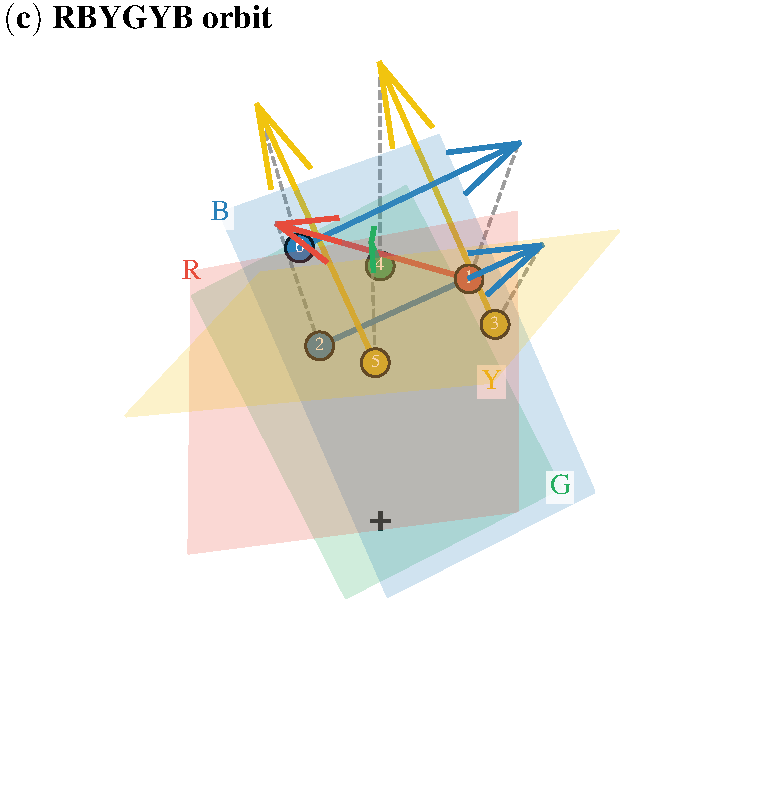
\includegraphics[width=0.5\textwidth]{figures/simon_rbygyb.pdf}
\caption{Simon RBYGYB sequence storage on a $K{=}4$, $N{=}3$ SCN with joint-optimised decoders and drives ($m=0.056$, $|\mu_2/\mu_1|=0.30$). Six numbered dots trace the period-$6$ word in firing order (1: R, 2: B, 3: Y, 4: G, 5: Y, 6: B), each on the bound plane $\Bsp_i$ of the firing neuron (translucent quadrilateral, coloured R/B/Y/G). Solid arrows: spike jumps $\yy\mapsto\yy+\DD_i$. Grey dashed: exponential decays back toward the origin (black cross).}
\label{fig:simon}
\end{SCfigure}

\subsubsection{Central pattern generators}\label{sec:apps-cpg}

Central pattern generators (CPGs) are small recurrent circuits that autonomously produce rhythmic, periodic activation of a fixed set of motor neurons with prescribed phase relationships, without requiring rhythmic drive from upstream areas \citep{marder2001central,kiehn2016decoding}. Concrete examples span the animal kingdom: the leech swim network, the lamprey spinal locomotor circuit, the mammalian spinal CPGs that coordinate walking, trotting, and other gaits, the pre-B\"{o}tzinger complex that generates the respiratory rhythm, and the brainstem mastication CPG \citep{kiehn2016decoding,grillner2006biological}. Across these systems the defining computational signature is the same. A compact network of a few tens of neurons, often only a handful, sustains a stereotyped periodic firing word in which each cell fires in a fixed order and at a fixed phase relative to the others, and the resulting spike sequence is what the downstream musculature reads out. A stable admissible periodic firing word $\sigma$ realized by an SCN is therefore a natural formal model of a CPG output, and the inverse problem of Section~\ref{sec:inverse} restated for this setting reads: design a small recurrent circuit whose intrinsic periodic attractor produces a target motor rhythm with a target inter-neuron phase pattern, using parameters that respect the reciprocal-inhibition architecture believed to underlie biological rhythm generation \citep{marder2001central}.

Two features of the framework match CPG biology particularly well. First, biological CPGs are known to operate with very small networks. The classical case is Graham Brown's half-center oscillator, in which two mutually inhibiting units alternate in bursts of activity; this is the $K=2$ case, and $K=3,4$ cover the more complex three- and four-phase patterns that underlie tetrapod gaits and swim undulations \citep{grillner2006biological,kiehn2016decoding}. The margin-based inverse solver of Section~\ref{sec:inverse-statement} is efficient precisely in this small-$K$ regime, where a handful of admissibility constraints on the return matrix $\vv{M}_\sigma$ fully pin down the geometry. Given a target rhythm, specified as a periodic firing word with prescribed inter-spike intervals, the solver returns decoders $\vv{D}$ and drives $\boldsymbol{\alpha}$ that make $\sigma$ a stable eigenvector of $\vv{M}_\sigma$ with subdominant eigenvalue ratios shrunk inside the unit circle by Theorem~\ref{thm:eigvec}. Second, cone preservation $\cos\psi_{ij}>0$ (Thm.~\ref{thm:cone}(a)) is exactly the reciprocal-inhibition mechanism identified by Graham Brown as the atomic building block of rhythm generation; the half-center oscillator is a natural $K=2$ instance.

\subsubsection{HVC and precisely timed spike sequences}\label{sec:apps-hvc}

In the singing zebra finch, RA-projecting neurons in HVC each emit an ultra-sparse burst, typically a single burst per song bout, at a stereotyped time locked to song onset; the downstream RA circuit reads this sparse code and produces the precisely timed motor pattern that drives the vocal muscles of the syrinx. Across renditions the timing of these events is reproducible at the millisecond scale, and analogous millisecond timing codes are documented across vertebrate motor behavior, from cortical vocal areas \citep{tang2014millisecond} to a broad range of skilled movements \citep{sober2018millisecond,pascual2024millisecond}. The biological problem posed by these observations is inverse in the sense used here: the firing code $\sigma$ is fixed by the animal's behavioural output, and the question is what recurrent substrate can hold that particular word as an intrinsic, self-sustaining pattern rather than as a transient response to an external teacher.

Existing spiking learning rules address only half of this problem. The Chronotron \citep{florian2012chronotron}, related tempotron variants, and the recurrent construction of \citet{memmesheimer2014learning} train a spiking cell (or a small network) to reproduce a prescribed spike train under a given input, treating the target pattern as a supervised signal rather than as an eigenstructure of the recurrence. The construction of Section~\ref{sec:inverse} fills exactly this gap: given a target precisely timed firing sequence $\sigma$, it returns decoders $\vv{D}$ and drives $\boldsymbol{\alpha}$ such that $\sigma$ is realized as the stable dominant eigenvector of the return matrix $\vv{M}_\sigma$, with admissibility margin $m(\boldsymbol{\alpha})>0$. The $3$--$5\%$ D-type tolerance of the constructed orbits comfortably brackets the millisecond-scale timing jitter reported in \citet{tang2014millisecond,sober2018millisecond}, so within the model, HVC/RA-like sparse codes sit inside the tolerance regime covered by Theorem~\ref{thm:eigvec} and the analytical robustness bound~\eqref{eq:tolerance}.

\subsubsection{Working memory: persistent, multistable, and continuous-attractor storage}\label{sec:apps-wm}

Adding auxiliary constraints to the same inverse objective turns the SCN into a working-memory substrate with three complementary storage regimes: persistent memory (no extra constraint), multistability (jointly optimize the margins of several target words), and continuous attractors (enforce a double dominant eigenvalue). All three coexist with the sequence-memory reading of Section~\ref{sec:apps-simon}, and a single $(\vv{D},\boldsymbol{\alpha})$ can realize several of them simultaneously.

 Every stable admissible limit cycle of the continuous-time SCN flow is invariant under the input shift
\begin{equation}\label{eq:shift-invariance}
\yy\mapsto\yy-\vv{c},\qquad\alpha_i\mapsto\alpha_i-\DD_i\cdot\vv{c},
\end{equation}
under which the orbit shape, period, firing word, and full Lyapunov spectrum (Theorem~\ref{thm:eigvec}) are all preserved. Setting $\vv{c}=0$ removes the input but leaves the realized word intact: the SCN persists the categorical memory (which of the countably many admissible words) by sustaining its limit cycle. Since stability and admissibility are open conditions on $(\vv{D},\boldsymbol{\alpha})$, this form of persistent memory is generic, requiring no codimension-1 fine-tuning of eigenvalues \citep{Park2023a}. Constant-input SCN orbits thereby act as structurally-stable quasi-periodic attractors, extending the line-attractor \citep{seung1996brain} and ring-attractor \citep{benyishai1995theory} tradition into the discrete-token setting.

 For fixed $(\vv{D},\boldsymbol{\alpha})$ the return map $\vv{M}_\sigma$ of every prescribed word carries its own dominant eigenvector, admissibility check, and basin of attraction (Section~\ref{sec:periodic}), so the initial condition selects which stored orbit is retrieved. For $K=2$ the piecewise projective map is a degree-$1$ circle homeomorphism (Proposition~\ref{prop:circle-homeo}) with a unique rotation number, and only one stable word coexists at each parameter value. For $K\geq 3$ the richer partition geometry can support several coexisting attractors at chosen parameters; the four-neuron Simon network of Section~\ref{sec:apps-simon} demonstrates this constructively, admitting a period-$6$ RBYGYB orbit (basin fraction ${\sim}83\%$ across $200$ random initial conditions) and a period-$2$ GR orbit (basin fraction ${\sim}17\%$). A cleaner symmetric instance is the pair of chirality-related orbits $\sigma=(1,2,3)$ and $\sigma=(1,3,2)$ on a $K=N=3$ symmetric SCN (Figure~\ref{fig:multi-chirality}); jointly optimizing the admissibility margins of a prescribed word set is the multi-word extension~\eqref{eq:multi-inverse} of the single-word solver. Empirically the dominant eigenvector is always the unique candidate that passes the admissibility check (Section~\ref{sec:periodic}); the non-dominant algebraic candidates fall outside the admissible region and are dynamically inaccessible. The basins are separated by the partition hyperplanes~\eqref{eq:partition} rather than by unstable periodic orbits, and the derivative discontinuities at those hyperplanes provide the repulsion that a smooth system would achieve through matched saddle indices.

\begin{SCfigure}[1.0][t]
\centering
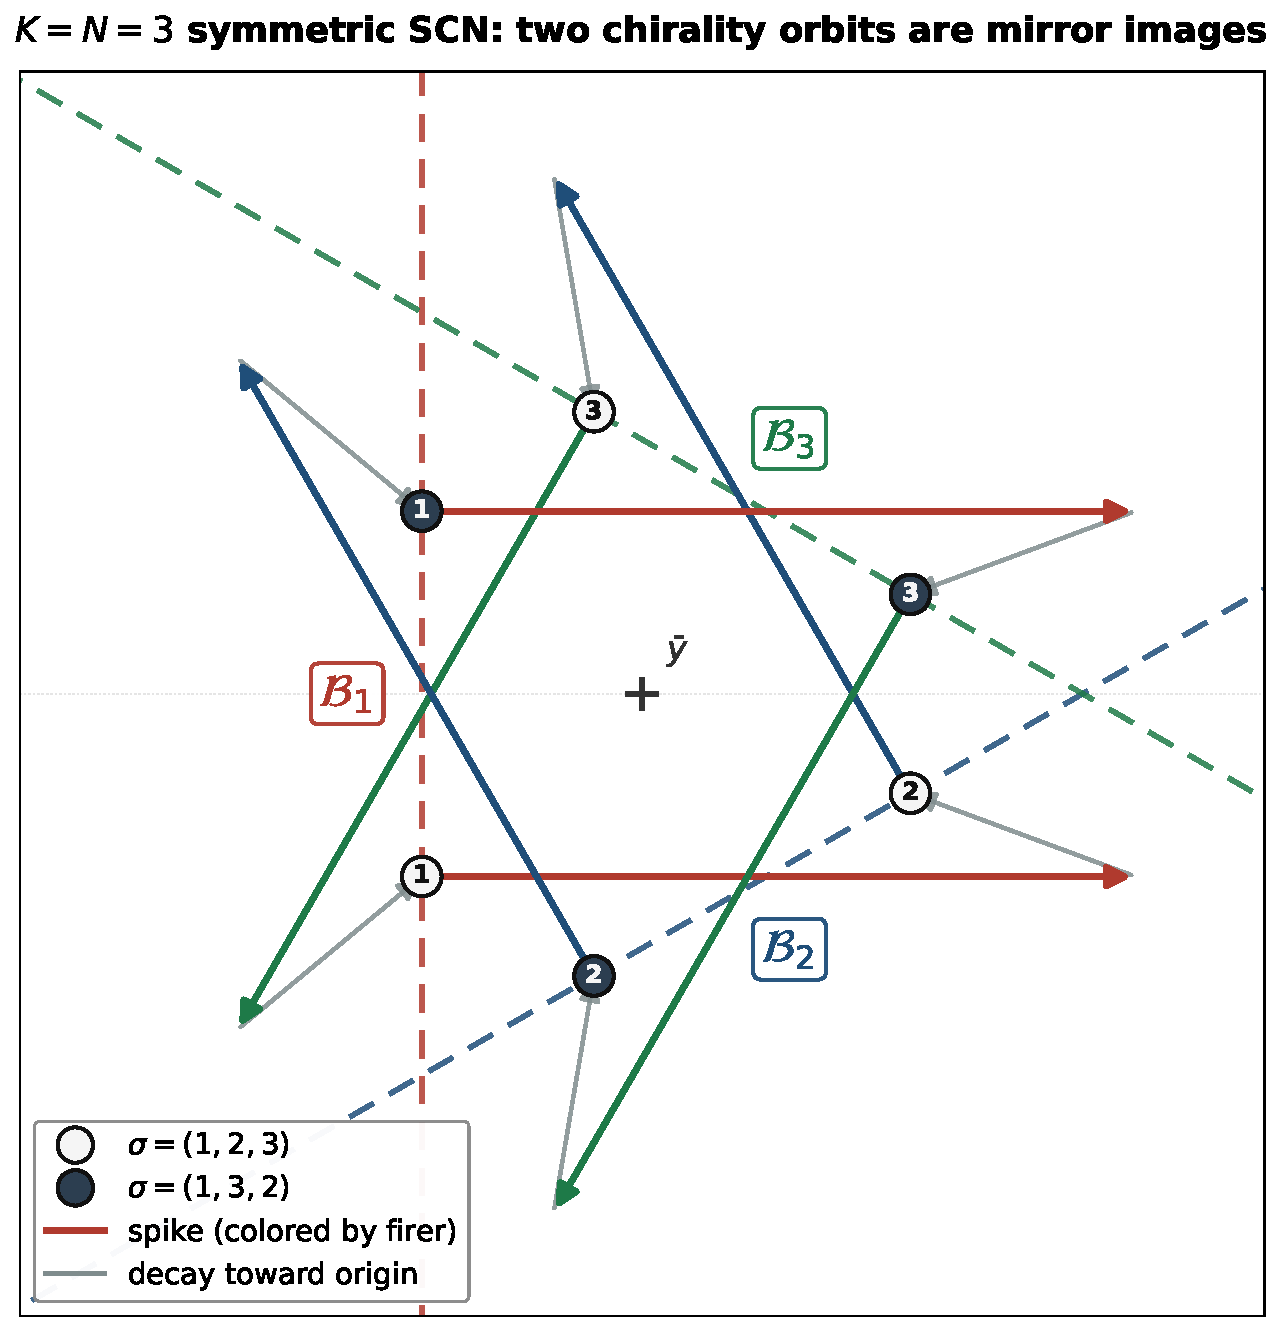
\includegraphics[width=0.45\textwidth]{figures/multistability_topdown}
\caption{Chirality multistability: two coexisting orbits $\sigma=(1,2,3)$ (light) and $\sigma=(1,3,2)$ (dark) of a symmetric $K=N=3$ SCN at $\alpha_i=0.7$, related by the $2\leftrightarrow 3$ reflection, viewed along the $(1,1,1)/\sqrt{3}$ axis. Coloured arrows: $\vv{D}_i$-spikes; grey arrows: decay toward the origin. Dashed slices: bounds $\mathcal{B}_j$. Both orbits share the same time-averaged readout $\bar{\vv{y}}$: the $S_3$ neuron-permutation symmetry that maps one orbit to the other forces both orbit means onto the fixed axis $\sum_j\vv{D}_j$ of the reflection (verified to machine precision, $\|\bar{\vv{y}}_A-\bar{\vv{y}}_B\|\approx 10^{-16}$).}
\label{fig:multi-chirality}
\end{SCfigure}

 The stability ratio $|\mu_2/\mu_1|$ of Theorem~\ref{thm:eigvec} controls the timescale of drift along the dominant eigenvector: as $|\mu_2/\mu_1|\to 1$ from below, second-eigenvector perturbations decay on ${\sim}L/\ln(|\mu_1/\mu_2|)$ steps, which can substantially exceed the orbit period. In the exact limit $\mu_1=\mu_2$ with a two-dimensional eigenspace, the fixed point is replaced by a one-parameter family of period-$L$ orbits sharing the same word $\sigma$ (Corollary~\ref{cor:edge-cases}), a \emph{line attractor} in the sense of \citet{seung1996brain}. The admissibility check~\eqref{eq:admissibility-check} restricts the family to a closed interval $[t_-,t_+]$ obtained explicitly from the tie conditions between the prescribed firer and its next-step competitors, each of which is linear in the family parameter. Joint optimization over $(\vv{D},\boldsymbol{\alpha})$ realizes this codimension-2 surface on a $K=N=3$ SCN for the period-3 word $\sigma=(1,2,3)$: at $\boldsymbol{\alpha}=(1.435,1.037,1.411)$ with $\mu_1=\mu_2=4.124$ (rank deficit ${\sim}10^{-13}$), the admissible interval is $[t_-,t_+]=[-0.145,+0.029]$ and direct SCN simulation from any $t$ inside it traces the prescribed orbit to floating-point precision. The codimension-2 surface is not robust to parameter perturbations (a generic perturbation of magnitude $\varepsilon$ splits the eigenvalues at first order, $|\mu_2/\mu_1|=1-C\varepsilon+O(\varepsilon^2)$), but its open $\varepsilon$-neighbourhood is the biologically relevant \emph{approximate}-CA regime: at $|\mu_2/\mu_1|=0.962$ on a $K=4$, $N=3$ solution, transverse perturbations halve every ${\sim}36$ spikes and persist for ${\sim}50$ cycles, corresponding to ${\sim}1.5$\,s at a membrane time constant of $\tau=10$\,ms and matching the timescale of biological working memory \citep{AnonSelfCite2024a}. An interactive 3D visualisation of the LA tube is provided in the supplementary material.


\section{Discussion}\label{sec:discussion}
%======================================================================

\paragraph{Summary.}
In summary, we have shown that the spike-and-decay dynamics of an SCN reduce exactly to a piecewise projective map on the disjoint union of spike-bound hyperplanes (Theorem~\ref{thm:projective}). Periodic firing patterns are eigenvectors of an $N{\times}N$ return matrix, and the orbit's full Lyapunov spectrum is read off in closed form from the eigenvalue ratios, one ratio per independent perturbation direction in the tangent space (Theorem~\ref{thm:eigvec}). The sign of the pairwise decoder cosines acts as a sharp order parameter (Theorem~\ref{thm:cone}): positive cosines leave a positive cone invariant and force the dynamics to contract in the Hilbert metric by Birkhoff--Hilbert contraction (Theorem~\ref{thm:cone}(a)), ruling out chaos; negative cosines break the cone invariance and permit positive Lyapunov exponents. The inverse problem of finding network parameters that realize a prescribed periodic firing word is recast as a semi-algebraic feasibility question with both an analytical solution for permutation words and a differentiable admissibility margin for general words.

Three implications for neuroscience follow directly. First, sequence working memory acquires a closed-form mechanism: retrieval is an autonomous limit cycle unfolded from the dominant eigenvector of $\vv{M}_\sigma$; the admissibility margin's shrinkage with word length gives a geometric mechanism for the $4{\pm}1$ capacity figure~\citep{cowan2001magical}, without decay, interference, or rehearsal (\S\ref{sec:apps-simon} discusses the caveat). Second, the cone constraint $\cos\psi_{ij}>0$ that prevents chaos (Theorem~\ref{thm:cone}) coincides exactly with the geometry that makes the connectivity $W_{ij}=-\DD_i^\top\DD_j$ uniformly inhibitory, so Dale's law for inhibition follows structurally from the cone-preserving regime; biological circuits operating near the cone boundary (mixed E/I, the regime supporting linear computation \citep{boerlin2013predictive,calaim2022geometry}) sit naturally near the edge of chaos. Third, multistability supports parallel sequence storage: a single $(\vv{D},\boldsymbol{\alpha})$ can simultaneously support many limit cycles, and varying the input $\xx$ navigates the devil's staircase (Theorem~\ref{thm:staircase}) to switch between them, yielding an analytical account of input-dependent sequence retrieval distinct from synfire-chain or attractor-network models.

Our work is built upon a connection between two separate strands of spiking-network theory. The projective reduction goes beyond the general-LIF event-based maps of \citet{monteforte2010dynamical,engelken2013dynamical} (see Intro): those live on the full $K$-dim membrane state and require simulation to discover orbits, whereas ours predicts them from a single $N{\times}N$ eigendecomposition. Reverse-engineering low-rank task-trained RNNs~\citep{sussillo2013blackbox,maheswaranathan2019universality,driscoll2024flexible} recovers analogous dynamical primitives empirically after training; we obtain the equivalent description analytically for the SCN architecture without training. Sequence-generation models based on synfire chains~\citep{abeles1991corticonics} or heteroclinic cycles~\citep{rabinovich2008transient} produce sequential firing but rely on fragile feedforward or saddle-connection architectures; our periodic attractors are robust eigenvector orbits with explicitly bounded basins. Finally, chaos in balanced networks under random connectivity~\citep{vreeswijk1996chaos} arises above an E/I balance threshold; we localize the analogous order--chaos transition geometrically to the sign of the smallest pairwise decoder cosine (Theorem~\ref{thm:cone}).

Beyond conceptual clarity, the reduction pays off computationally. Once the $K^2$ transition matrices $\vv{M}_{j\leftarrow i}\in\RR^{N\times N}$ are precomputed from the decoder geometry (one-time cost $O(K^2 N^2)$), each spike step reduces to evaluating $K$ decay factors (dot products) and one matrix-vector product, with no ODE solver or root finding required. For periodic-orbit prediction, the entire orbit is determined by a single $N{\times}N$ eigenvector computation regardless of orbit length $L$, bypassing transient simulation. A direct head-to-head benchmark on random $(K,N)$ systems shows the eigenvector method delivers a ${\sim}60$--$70\times$ wall-clock speedup over forward simulation across $K=3$--$20$ (Table~\ref{tab:bench}). This advantage grows with the stability ratio $|\mu_2/\mu_1|\!\to\!1$: orbits whose convergence is slow, which would require correspondingly longer simulation runs, are still recovered by a single $N{\times}N$ eigendecomposition in the same time. The method is complementary to general-purpose event-based simulators such as SparseProp~\citep{engelken2023sparseprop}, which achieve efficiency through sparse connectivity and run on networks of arbitrary topology but still require forward integration to discover orbits. The projective structure thus enables a ``compile-then-query'' workflow: precompile the transition matrices, then answer questions about orbits, stability, and bifurcations algebraically.

\begin{table}[t]
\centering
\caption{Wall-clock benchmark: forward simulation vs.\ the eigenvector method for periodic-orbit prediction. Simulation runs $20{,}000$ warmup steps and records one period; the eigenvector path runs a $\leq 300$-step word-detection sweep and one $N{\times}N$ eigendecomposition. Median over 25 trials (Python/NumPy, single CPU).}\label{tab:bench}
\begin{tabular}{rrrrrrr}
\toprule
$K$ & $N$ & $L$ & $|\mu_2/\mu_1|$ & Simulation (ms) & Eigenvector (ms) & Speedup \\
\midrule
3  & 2  & 2 & 0.508 & 371  & 5.3  & 70$\times$ \\
5  & 3  & 2 & 0.340 & 478  & 7.8  & 62$\times$ \\
8  & 4  & 2 & 0.844 & 577  & 8.9  & 65$\times$ \\
15 & 8   & 9 & 0.015 & 925   & 14.6  & 63$\times$ \\
20 & 10  & 2 & 0.644 & 1011  & 16.1  & 63$\times$ \\
10 & 50  & 18 & 0.241    & 432   & 1.0   & 415$\times$ \\
20 & 100 & 26 & $<10^{-3}$ & 3771  & 11.6  & 326$\times$ \\
\bottomrule
\end{tabular}
\end{table}

The bottom two rows of Table~\ref{tab:bench} push the benchmark into network sizes used in modern cortical SCN models. We use cone-cap decoders (decoders drawn uniformly from a spherical cap of a specified \emph{half-angle}, i.e.\ the maximum angular deviation from a reference direction, around a reference direction tuned so that the resulting min pairwise cosine remains positive but small, exploiting concentration of measure at high $N$) and uniform drives; forward simulation discovers a non-trivial admissible periodic orbit in both cases. At $N=50, K=10$ a \emph{period-18} word visits $7$ of the $10$ neurons ($70\%$ coverage), at a cone with min pairwise cosine $\approx 0.08$ (half-angle $\approx 1.16$ rad) and $|\mu_2/\mu_1| = 0.24$; the word is $(9,3,1,7,8,1,9,3,1,8,0,4,7,1,9,3,8,1)$. At $N=100, K=20$ a \emph{period-26} word visits $7$ distinct neurons, at a tighter cone (half-angle $0.4$ rad) and $|\mu_2/\mu_1| < 10^{-3}$. The eigenvector method of Theorem~\ref{thm:eigvec} confirms each orbit in $1$--$12$\,ms; forward simulation takes ${\sim}432$\,ms ($N=50$) and ${\sim}3.8$\,s ($N=100$), giving ${\sim}415\times$ and ${\sim}326\times$ speedups respectively.

These cortical-scale numbers expose a cone-width trade-off intrinsic to the framework. Wider cones (half-angle approaching $\pi/2$, min cosines near zero) admit substantially richer orbits at the cost of slower transverse contraction ($|\mu_2/\mu_1|$ closer to 1, hence closer to the chaos boundary of Theorem~\ref{thm:cone}(b)). The $N=50, K=10$ period-$18$ result above uses a near-boundary cone (min cos $0.08$); the $N=100, K=20$ result uses a tight cone (min cos $0.84$) and its orbit is sparser but more strongly stable. Networks that need to express many neurons in a single periodic orbit should operate near the cone boundary; networks that need maximally robust storage should operate well inside the cone. Basin surveys show the same dichotomy. The tight-cone $N=100, K=20$ network has a \emph{single} attractor across $800$ random initial conditions (all converge to the same canonical period-$26$ word), while the wide-cone $N=50, K=10$ network exhibits \emph{$23$ distinct stable attractors} in a $400$-IC survey: the dominant period-$18$ orbit holds basin fraction $\approx 12\%$, several period-$1$ self-loops and many medium-period orbits coexist, and the union of distinct firers across the atlas covers all $10$ neurons. Multistability for $K\geq 3$ is therefore parameter-dependent; it is suppressed at tight cones (basins concentrate onto one dominant orbit) and emerges in wide-cone regimes near the chaos boundary, but is not generic in either limit, and whether a given $(N, K, \text{cone width})$ tuple supports it requires empirical exploration.

The framework makes four concrete predictions for cortical circuits that hold sequences in working memory. (i)~\textbf{The robust code is the rotation number, not the spike-by-spike word.} The exact firing word does not survive realistic noise ($3$--$5\%$ tolerance vs.\ $10$--$30\%$ biological noise; \S\ref{sec:apps-simon}), but the firing ratio $\rho$ is constant on each rational mode-locked plateau of the devil's staircase (Theorem~\ref{thm:staircase}) and is therefore robust to all sub-bifurcation noise. This is a sharp prediction distinguishing the framework from synfire-chain models, which require spike-by-spike precision: \emph{sequence-encoding circuits should be robust at the level of population firing ratios but fragile at the level of exact spike order}; an observation that population firing ratios drift with sub-bifurcation input jitter while spike order remains preserved would invalidate this account. Parametric input shifts should further produce devil's-staircase bifurcations in population firing ratios (Theorem~\ref{thm:staircase}), with plateau widths obeying the Farey-mediant ordering and shrinking as $1/q^2$ for orbits of period $q$. (ii)~In multistable regimes, input perturbations should produce hysteretic switching between coexisting sequence attractors, with the switching geometry determined by the partition hyperplanes~\eqref{eq:partition}; absence of hysteresis where the theory places multiple stable orbits would be inconsistent with the framework. (iii)~The dominant eigenvalue ratio $|\mu_2/\mu_1|$ predicts the timescale of post-perturbation reconvergence to the stored sequence (Theorem~\ref{thm:eigvec}), observable in single-trial spike-time alignment; a reconvergence timescale uncorrelated with $|\mu_2/\mu_1|$ estimated from the recorded orbit would invalidate the eigenvector picture. (iv)~The cone dichotomy of Theorem~\ref{thm:cone} predicts that introducing excitatory connectivity to an otherwise inhibitory sequence-encoding circuit drives it toward irregular, unpredictable firing once the smallest pairwise decoder cosine crosses zero; observing a smooth continuation of stable sequential firing across that crossing would contradict the cone prediction.

Several limitations bound the scope of the results. The exact reduction requires uniform leak rates, instantaneous spikes, and constant input. Mode-locked words survive ${\sim}3$--$5\%$ parameter perturbation in noise scans, in agreement with the tolerance bound~\eqref{eq:tolerance} obtained from Davis--Kahan eigenvector perturbation theory \citep{davis1970rotation,stewart1990matrix}; see Theorem~\ref{thm:supp:davis-kahan}; finite spike width is benign, rescaling the drive without changing the word. The constant-input assumption is partially addressed by the input-switching mechanism, since different $\xx$ select different words via the devil's staircase (Theorem~\ref{thm:staircase}), but genuinely time-varying $\xx$ breaks the decay-ray structure underlying Theorem~\ref{thm:projective}, and a Floquet-style extension to slowly varying inputs remains open. The admissibility margin is differentiable but has local optima for $K\geq 3$, requiring global search; with simplex decoders the inverse solver succeeds up to $K=6$ (margin $m\approx 0.005$, time ${\sim}10$\,s), beyond which partition regions become prohibitively narrow. We have not analyzed learning or plasticity: the network parameters here are constructed, not learned.

Several natural extensions of the framework remain open, starting with the forward direction. The construction of Section~\ref{sec:inverse} solves the inverse problem, but the reverse question is asymmetric. Fixing $(\vv{D},\boldsymbol{\alpha})$, which firing words appear as stable admissible periodic orbits of the resulting network? For $K=2$ the answer is complete: the Sturmian bijection of Theorem~\ref{thm:classification} identifies the realized words with the mechanical Sturmian sequences of Remark~\ref{rem:sturmian} (a Morse--Hedlund~\citep{morse1938symbolic,morse1940symbolic} reading of the return map (Theorem~\ref{thm:supp:morse-hedlund})), and the rotation number is a full invariant of the devil's-staircase plateau structure (Theorem~\ref{thm:staircase}). For $K\geq 3$ the picture is open. Conjecture~\ref{conj:sofic} posits that the realized words form a sofic shift over $\{1,\ldots,K\}$; a natural route toward it is to build a finite presentation from the transition graph on the partition hyperplanes~\eqref{eq:partition} and to check that it matches the shift generated numerically by the return map. Two substructures organize the finer questions: whether the scalar rotation number generalizes to a rotation vector $\boldsymbol{\rho}=(\rho_1,\ldots,\rho_K)$ that still parametrizes plateaus or the staircase becomes genuinely higher-dimensional; and whether the plateau structure remains a devil's staircase along one-parameter deformations of $\boldsymbol{\alpha}$ or breaks into a coexistence of words once the cone-preserving regime is left. Closing this forward direction would turn the SCN framework into a fully analytic map from connectivity to asymptotic firing behavior.

Beyond that forward direction, three extensions of the framework stand out. First, a sharper characterization of the order--chaos onset as decoder cosines become negative: is the transition of Theorem~\ref{thm:cone} generically continuous (as suggested by Figure~\ref{fig:chaos}a) or discontinuous, and is there a universal scaling for $\lambda_{\max}$ near the cone boundary? Second, characterizing the set of realizable firing words for fixed $(N,K_E,K_I)$ as a \emph{subshift of finite type}: the admissibility conditions~\eqref{eq:partition} define a transition graph, and the realizable words are the paths through it; counting these and computing the topological entropy of the symbolic dynamics is a natural next step. Third, engineering continuous attractors via deliberate eigenvalue collisions ($|\mu_2/\mu_1|\to 1$), that is, the line-attractor edge case (Corollary~\ref{cor:edge-cases}), to obtain analog working memory in the spike-coding paradigm. Prior work has shown~\citep{AnonSelfCite2024a} that vanilla RNNs cannot perfectly learn continuous-input integration (their trained dynamics form an approximate continuous attractor as a slow invariant manifold rather than an exact integrator); the projective framework here gives an analytical handle on the related question of \emph{which} periodic dynamics SCNs can realize, suggesting that the inverse-problem viewpoint may extend to characterizing constructible attractor structures more generally. Extending the projective machinery to networks with multiple latent boundaries~\citep{podlaski2024approximating} and to time-varying inputs would substantially broaden the applicability of the framework.

\paragraph{Acknowledgments.}
This work was supported by NIH RF1-DA056404 and the Portuguese Recovery and Resilience Plan (PRR), through project number 62, Center for Responsible AI, and by Portuguese national funds through FCT~--~Funda\c{c}\~ao para a Ci\^encia e a Tecnologia, in the context of project UIDB/04443/2020.

\paragraph{Code availability.}
All code reproducing the figures and numerical results is released at an anonymised repository (URL withheld for double-blind review; the code accompanies this submission as supplementary material and will be de-anonymised at acceptance).
% The repository contains the core piecewise projective map implementation (transition matrices, return-map composition, eigenvector orbits, partition-boundary checks), the inverse solver, and a Python script per figure. 
%See the repository's \texttt{README} for the mapping between scripts and paper figures, and \texttt{requirements.txt} for the small NumPy/SciPy/matplotlib dependency set.


\newpage
\bibliographystyle{plainnat}
\bibliography{all_ref,catniplab}

\newpage
\FloatBarrier

% -- appended supplement (auto-merged; keep single-source scn_supplementary.tex for standalone build) --
% =====================================================================
% scn_appendices.tex -- self-contained appendix fragment.
% Auto-extracted from scn_supplementary.tex (single source of truth for
% standalone supplement build). Do not edit this file directly; edit
% scn_supplementary.tex and re-extract if the merged paper appendices
% need updating.
% =====================================================================

\appendix

\section{Worked examples (main text \S 2.5)}\label{app:worked-examples}


We set $N{=}K{=}2$ with decoders at angle $\psi=0.4\pi$, drives $\alpha_1=1.0$, $\alpha_2=0.49$. The return map for the period-7 word $\sigma=(1,1,2,1,1,1,2)$ has eigenvalues $\mu_1\approx 12.60$, $\mu_2\approx 1.35$, giving $\xi^*\approx 0.717$ and $|\mu_2/\mu_1|\approx 0.107<1$ (stable). Figure~\ref{fig:overview-supp} shows the geometry, orbit, and devil's staircase.

\begin{figure}[t]
\centering
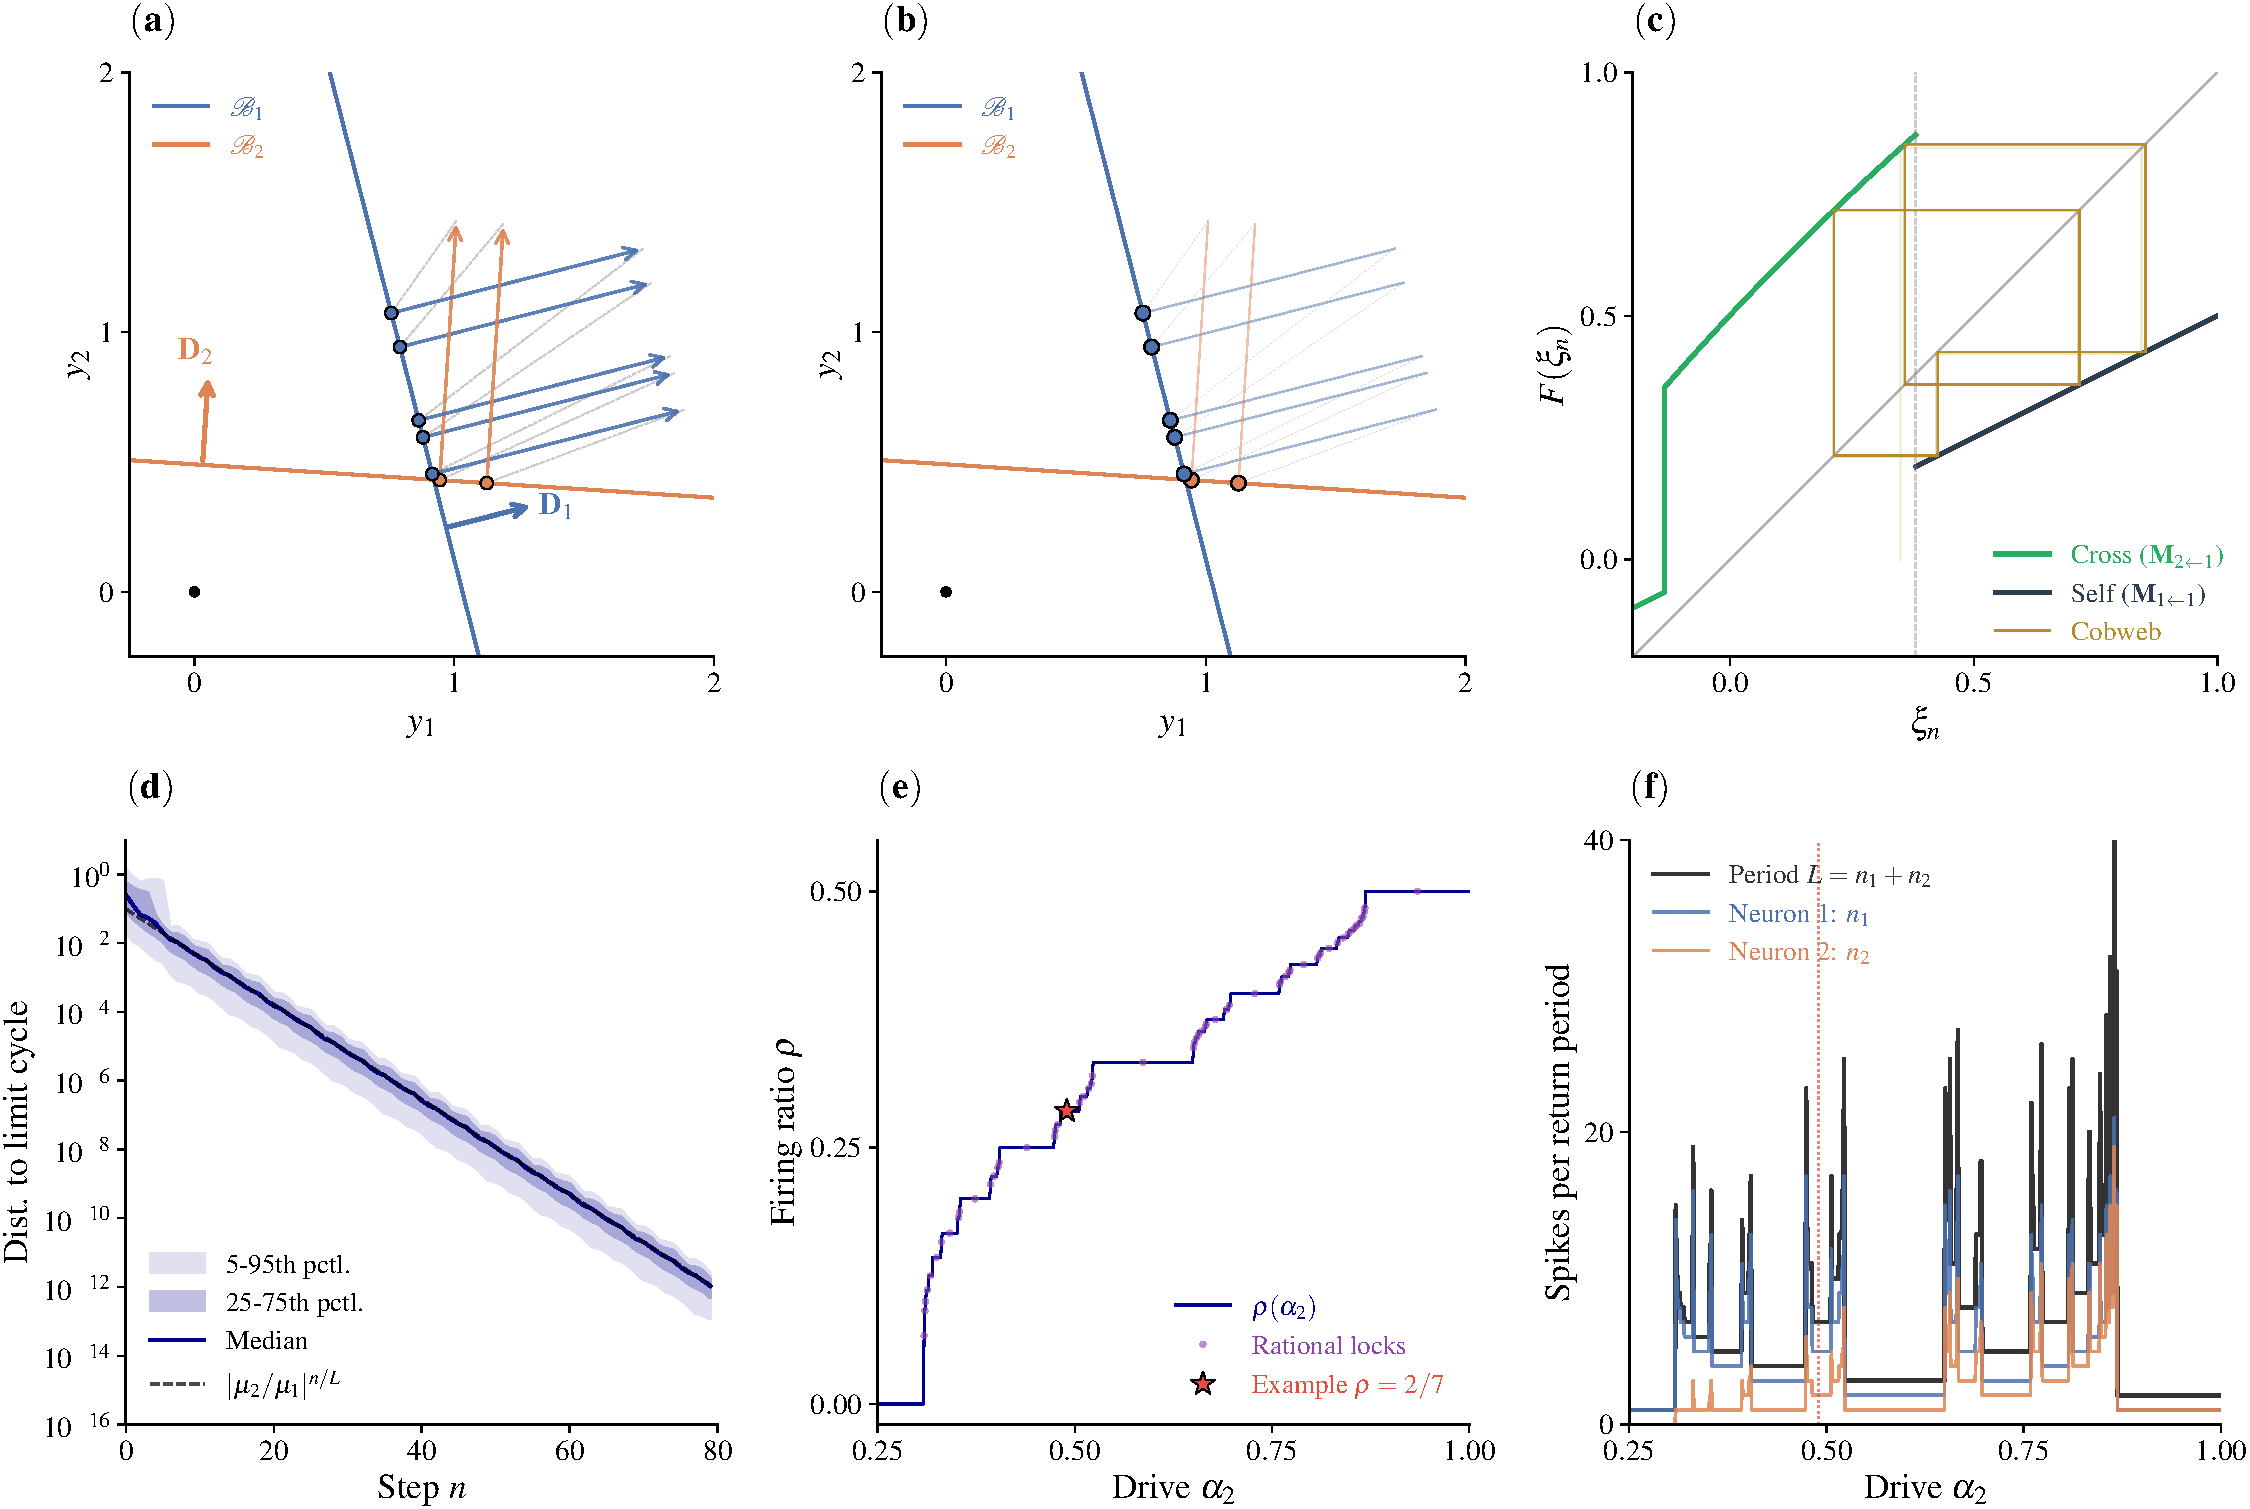
\includegraphics[width=\textwidth]{figures/scn_word_example.pdf}
\caption{Overview of SCN dynamics for $N=K=2$, $\psi=0.4\pi$.
\textbf{(a)}~Geometry: decoder vectors $\DD_1,\DD_2$, spike bounds $\Bsp_1,\Bsp_2$, and one period of the converged orbit (spike arrows and decay segments from the eigenvector-predicted positions).
\textbf{(b)}~Period-7 orbit ($\sigma=0010001$, $\alpha_1=1$, $\alpha_2=0.49$): all seven positions predicted by the dominant eigenvector of $\vv{M}_\sigma$ (colored dots), with spike and decay connections.
\textbf{(c)}~Cobweb diagram of the first-return map $F_{\!\Bsp_1}:\Bsp_1\to\Bsp_1$ (the return map to $\Bsp_1$, distinct from the full-cycle map $F$ of Eq.~\eqref{eq:F-from-M}). Two M\"obius branches: cross-transition (red, $\xi<\xi_{\mathrm{part}}$) and self-transition (blue, $\xi\geq\xi_{\mathrm{part}}$). The green cobweb converges from $\xi_0=1.3$ to the period-$5$ cycle of $F_{\!\Bsp_1}$ (the $5$ points of the underlying period-$7$ orbit that lie on $\Bsp_1$).
\textbf{(d)}~Devil's staircase: spike-based firing ratio $\rho_{\mathrm{spike}}=k/(q+k)$ vs.\ $\alpha_2$ (see Remark~\ref{rem:rho-conventions}), plotted on $[0,\tfrac{1}{2})$ rather than the $[0,1)$ range of the rotation-number staircase $\rho_F=k/q$ of Theorem~\ref{thm:staircase}(iii); the two staircases are related by the monotone bijection $\rho_{\mathrm{spike}}=\rho_F/(1+\rho_F)$, so the plateau structure is identical up to rescaling. Purple dots mark each mode-locked plateau. The star marks the operating point of panels~(a--c) at $\rho_{\mathrm{spike}}=2/7$ (equivalently, return-map rotation number $\rho_F=2/5$).}
\label{fig:overview-supp}
\end{figure}


The construction extends to $N{=}K{=}3$, where the $3\times 3$ return map has two stability ratios to check (Appendix~\ref{app:numerics}).





\section{Three-dimensional example (main text \S 3.4)}\label{app:3d-example}


We illustrate the framework on a $K=3$, $N=3$ system with decoders arranged symmetrically about the $[1,1,1]^\top/\sqrt{3}$ axis (pairwise cosine $\cos\psi_{ij}=0.507$, all-inhibitory cone) and drives $\boldsymbol{\alpha}=(1.0,0.9,0.7)$. A short simulation identifies the period-$L=11$ word $\sigma=(2,1,3,2,1,2,1,3,1,2,1)$ with firing ratios $(\rho_0,\rho_1,\rho_2)=(5/11,4/11,2/11)$; composing the eleven transition matrices gives a $3{\times}3$ return map whose dominant eigenvector predicts all eleven orbit points exactly (Figure~\ref{fig:3d}a,b). The tangent space is two-dimensional, so stability is determined by two eigenvalue ratios, $|\mu_2/\mu_1|=0.015$ and $|\mu_3/\mu_1|=0.008$; convergence from 500 random initial conditions decays at the predicted rate $|\mu_2/\mu_1|^{n/L}$ per step and reaches machine precision within ${\sim}97$ steps, matching $L\log(10^{-16})/\log|\mu_2/\mu_1|$ (Figure~\ref{fig:3d}c).

\begin{figure}[!ht]
\centering
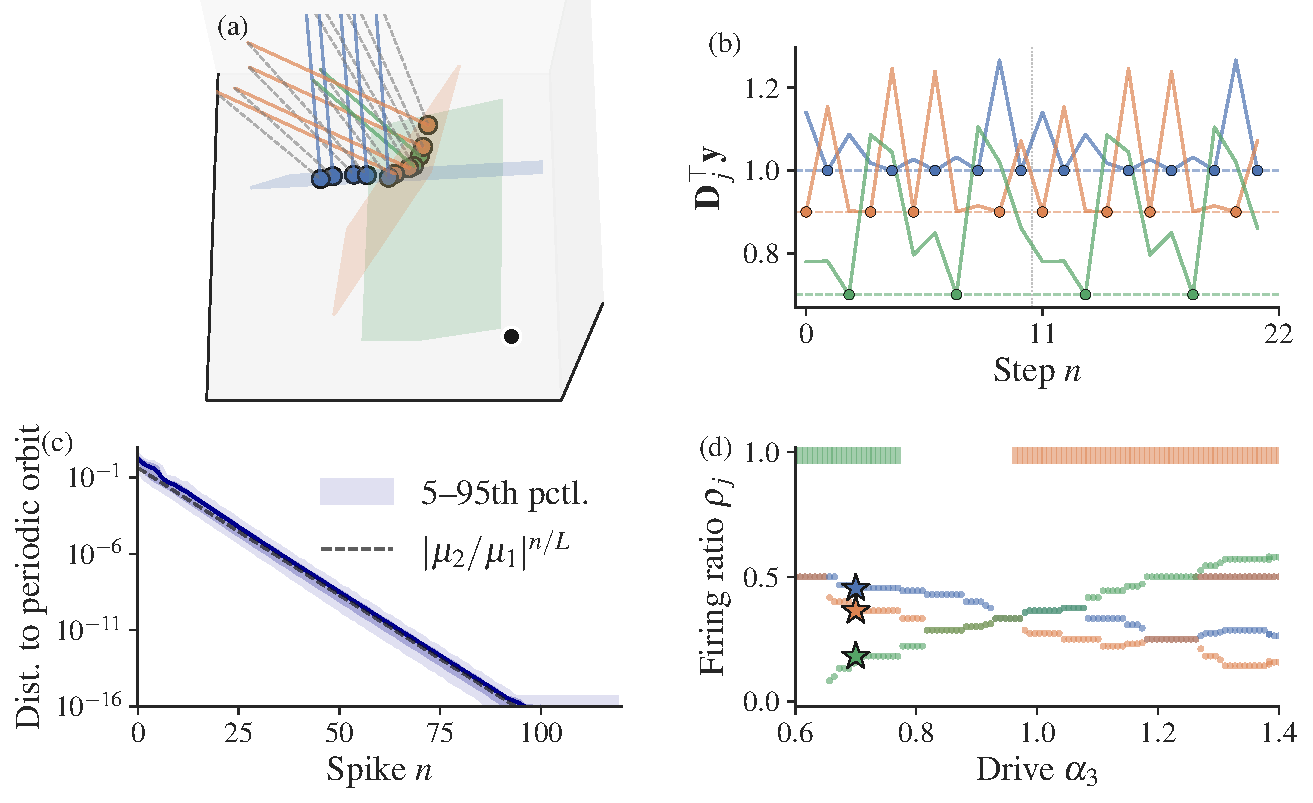
\includegraphics[width=\textwidth]{figures/fig_3d_example.pdf}
\caption{Three-neuron example ($K{=}3$, $N{=}3$, $\boldsymbol{\alpha}=(1.0,0.9,0.7)$, $\cos\psi_{ij}=0.507$).
\textbf{(a)}~Geometry: three spike bounds $\Bsp_1$ (red), $\Bsp_2$ (blue), $\Bsp_3$ (green) with the period-11 eigenvector orbit (colored dots), with spike arrows and decay segments connecting consecutive orbit positions in firing order. Black dot: origin of $\RR^3$.
\textbf{(b)}~Converged firing pattern over two periods: $\DD_j^\top\yy$ traces with the firing neuron at each step marked as a colored dot at the threshold $\alpha_j$ (dashed line). Traces of $\DD_j^\top\yy$ between successive firings of neuron~$j$ remain above $\alpha_j$ because each spike of neuron~$j$ instantaneously raises $\DD_j^\top\yy$ from $\alpha_j$ to $\alpha_j{+}1$ (since $\|\DD_j\|{=}1$), after which it decays exponentially back toward $\alpha_j$ before the next spike of neuron~$j$. The dotted vertical line at $n=L=11$ marks the period boundary.
\textbf{(c)}~Convergence to the periodic orbit from 500 random initial conditions (filtered to the 90\% reaching the period-11 orbit): mean (dark) with 25--75th and 5--95th percentile bands; dashed line is the analytical decay $|\mu_2/\mu_1|^{n/L}$.
\textbf{(d)}~Devil's staircase: the three firing ratios $\rho_0$ (red), $\rho_1$ (blue), $\rho_2$ (green) as $\alpha_3$ varies. Coloured tick markers at $\rho{=}1$ mark $\alpha_3$ ranges where the corresponding neuron's self-trapping orbit ($\rho_j{=}1$) coexists with the mixed orbit; stars mark the working point $\boldsymbol{\alpha}=(1.0,0.9,0.7)$.}
\label{fig:3d}
\end{figure}

\paragraph{Multistability and persistent staircase.}
About 10\% of initial conditions converge instead to a self-trapping fixed point on a single bound ($\sigma=2$, $\rho_2=1$); analogous self-trapping orbits on $\Bsp_1$ and $\Bsp_2$ coexist across the full parameter range, with basins delineated by the partition hyperplanes~\eqref{eq:partition}. Varying any of $\alpha_1,\alpha_2,\alpha_3$ at fixed values of the other two produces a devil's-staircase structure in all three firing ratios simultaneously (subject to $\rho_0+\rho_1+\rho_2=1$; Figure~\ref{fig:3d}d and Figure~\ref{fig:3d_staircases}); the self-trapping orbits coexist with the mixed orbit at every parameter value, so multistability is a persistent feature of $K\geq 3$, not a fine-tuned artifact.

\paragraph{What changes from $K=2$.}
Three new features distinguish the $K\geq 3$ regime: (i)~$N-1$ eigenvalue ratios to check rather than one (Theorem~\ref{thm:eigvec}); (ii)~partition boundaries on each bound are affine hyperplanes rather than points, making the bifurcation structure richer than a circle homeomorphism and breaking the $K=2$ uniqueness; (iii)~multistability between mixed and self-trapping orbits, while not generic, becomes possible at appropriate parameters.

\begin{figure}[!ht]
\centering
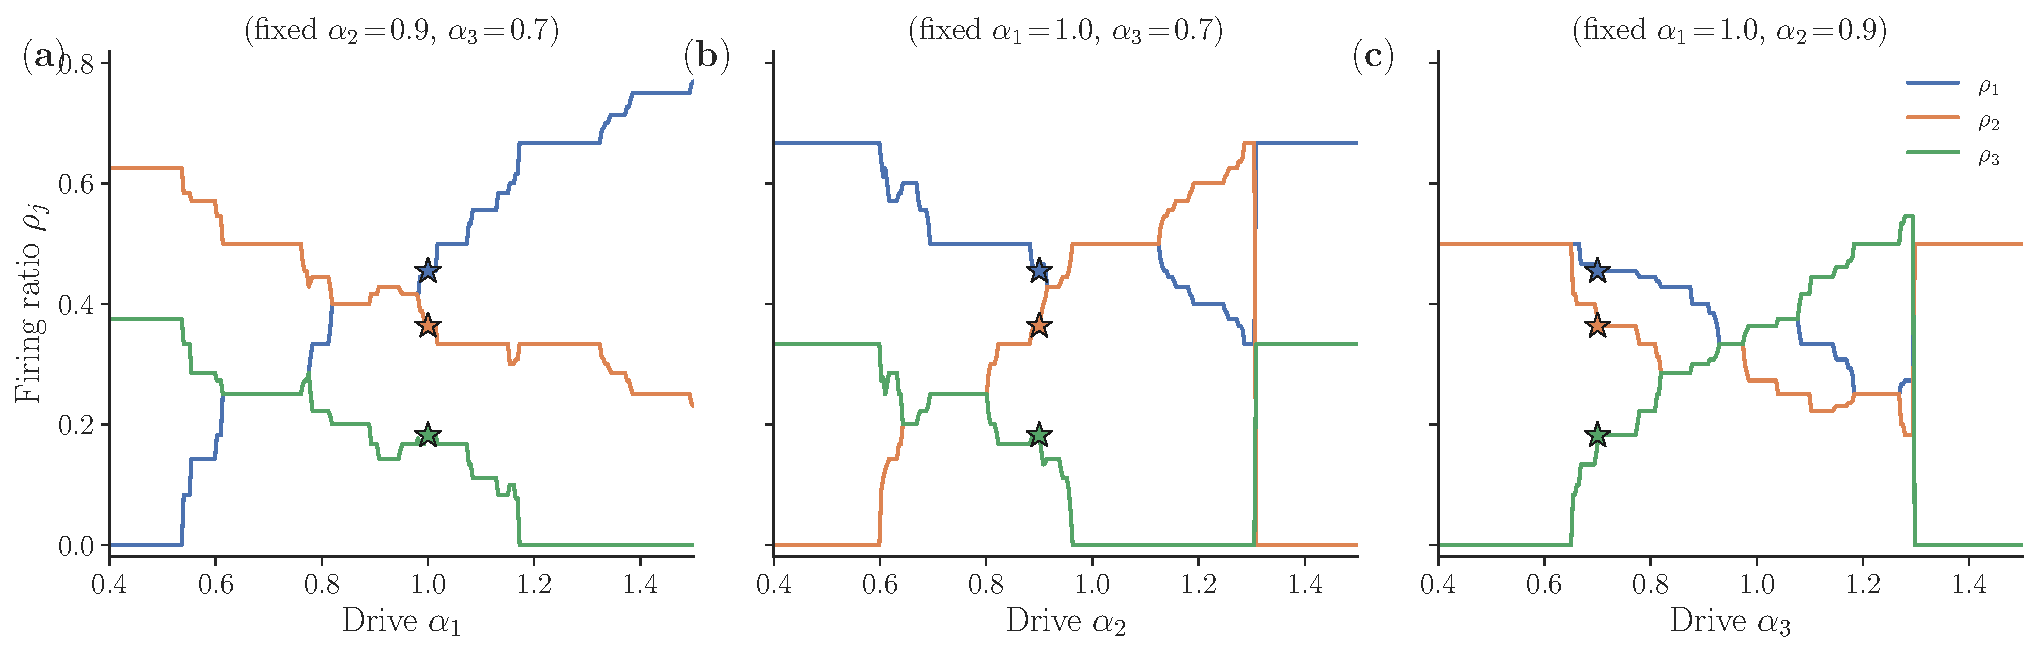
\includegraphics[width=\textwidth]{figures/fig_3d_staircases.pdf}
\caption{Devil's staircases for the three-neuron system, scanning each 
drive individually.
\textbf{(a)}~Varying $\alpha_1$ (fixed $\alpha_2{=}0.9$, 
$\alpha_3{=}0.7$).
\textbf{(b)}~Varying $\alpha_2$ (fixed $\alpha_1{=}1.0$, 
$\alpha_3{=}0.7$).
\textbf{(c)}~Varying $\alpha_3$ (fixed $\alpha_1{=}1.0$, 
$\alpha_2{=}0.9$).
In each panel, the three firing ratios $\rho_0+\rho_1+\rho_2=1$ 
redistribute through mode-locked plateaus as the varied drive 
increases. Stars mark the common working point 
$\boldsymbol{\alpha}=(1.0,0.9,0.7)$.}
\label{fig:3d_staircases}
\end{figure}


\section{Higher-dimensional verification (main text \S 3.5)}\label{app:highd-verif}


The reduction is exact for any $(K,N)$. Table~\ref{tab:highd} verifies this on 13 random configurations spanning square ($K=N$), underdetermined ($K<N$), and overdetermined ($K>N$) regimes: in each case the dominant eigenvector of $\vv{M}_\sigma$ predicts every orbit point to machine precision ($\|\text{err}\|_\infty<10^{-14}$), and the Lyapunov ratio $|\mu_2/\mu_1|$ is read off directly from the eigendecomposition. Further numerical details and the specific firing words are reported in Appendix~\ref{app:highd}.

\begin{table}[t]
\centering
\caption{Eigenvector orbit prediction verified across dimensions.  
For each $(K,N)$ configuration, a periodic orbit is found by simulation, 
the return map $\vv{M}_\sigma\in\RR^{N\times N}$ is assembled as a 
product of $L$ transition matrices, and its dominant eigenvector predicts 
all $L$ orbit points.  The prediction error 
$\|\text{theory}-\text{sim}\|_\infty$ is at machine precision in all 
cases.  $K_{\text{act}}$: number of neurons that actively fire in the 
orbit.}\label{tab:highd}
\begin{tabular}{rr rrr rr}
\toprule
$K$ & $N$ & $L$ & $K_{\text{act}}$ & $\|\text{err}\|_\infty$ 
& $|\mu_2/\mu_1|$ & $\vv{M}_\sigma$ \\
\midrule
\multicolumn{7}{l}{\emph{Square ($K{=}N$)}} \\
 2 &  2 &   2 &  2 & $< 10^{-15}$ & 0.19 & $2{\times}2$ \\
 3 &  3 &   3 &  2 & $4{\times}10^{-16}$ & 0.07 & $3{\times}3$ \\
 4 &  4 &   8 &  2 & $3{\times}10^{-16}$ & 0.01 & $4{\times}4$ \\
 8 &  8 &   4 &  3 & $7{\times}10^{-16}$ & 0.16 & $8{\times}8$ \\
10 & 10 &   2 &  2 & $1{\times}10^{-15}$ & 0.42 & $10{\times}10$ \\
\midrule
\multicolumn{7}{l}{\emph{Underdetermined ($K{<}N$)}} \\
 2 &  5 &   2 &  2 & $7{\times}10^{-16}$ & 0.27 & $5{\times}5$ \\
 3 & 10 &   5 &  2 & $4{\times}10^{-16}$ & 0.11 & $10{\times}10$ \\
 4 & 20 &   3 &  2 & $6{\times}10^{-16}$ & 0.15 & $20{\times}20$ \\
 5 & 50 &   8 &  4 & $5{\times}10^{-16}$ & 0.01 & $50{\times}50$ \\
\midrule
\multicolumn{7}{l}{\emph{Overdetermined ($K{>}N$)}} \\
 5 &  2 &   2 &  2 & $7{\times}10^{-16}$ & 0.63 & $2{\times}2$ \\
10 &  3 &   7 &  2 & $3{\times}10^{-16}$ & 0.07 & $3{\times}3$ \\
20 &  5 &   2 &  2 & $5{\times}10^{-16}$ & 0.41 & $5{\times}5$ \\
50 & 10 &   3 &  3 & $6{\times}10^{-16}$ & 0.36 & $10{\times}10$ \\
\bottomrule
\end{tabular}
\end{table}


\section{Chaos with opposing decoders: proof of Theorem~\ref{thm:cone}(b) and comparisons (main text \S 3.6)}\label{app:chaos-details}

\begin{proof}[Proof of Theorem~\ref{thm:cone}(b)]
(a)~Suppose $\yy\in\mathcal{C}$, i.e.\ $\DD_\ell^\top\yy>0$ for every $\ell$. After neuron $i$ fires, $\yy^+=\yy+\DD_i$ and $\DD_\ell^\top\yy^+=\DD_\ell^\top\yy+\cos\psi_{\ell i}$, which is positive for every $\ell$ because both summands are positive by hypothesis. The exponential decay $\yy\mapsto e^{-\lambda\tau}\yy$ scales positively, so it preserves $\mathcal{C}$. Hence every transition $\vv{M}_{j\leftarrow i}$ maps $\mathcal{C}$ into itself. By Birkhoff's theorem for linear maps of positive cones, the projective action on $\mathcal{C}$ is a strict contraction in the Hilbert metric, with contraction ratio bounded by $\tanh(\Delta/4)$ where $\Delta$ is the projective diameter of the image cone. Successive transitions have uniformly bounded images (the spike adds the fixed vector $\DD_i$ to a state already in a bounded region of $\mathcal{C}$), so $\tanh(\Delta/4)$ is bounded away from~$1$ uniformly over the orbit. The return map $\vv{M}_\sigma$ is therefore a uniform strict contraction in the Hilbert metric, and by Theorem~\ref{thm:eigvec} all Lyapunov multipliers satisfy $|\mu_k/\mu_1|<1$. The maximal Lyapunov exponent of any trajectory, computed as a Birkhoff time average of $\log|\mu_2/\mu_1|$ along the orbit, is therefore strictly negative on every periodic orbit and non-positive in general.

(b)~We exhibit an SCN with positive \emph{topological entropy} of its symbolic dynamics: the exponential growth rate $h_{\text{top}}(\Sigma)=\lim_{L\to\infty}\frac{1}{L}\log_2 N_L$, where $N_L$ is the number of distinct length-$L$ blocks appearing in admissible firing sequences. Positive topological entropy implies positive metric entropy and hence chaos. Take $K=4$ neurons in $N=3$ with decoders
$\DD_1\approx(0.566,-0.791,-0.233)$,
$\DD_2\approx(0.748,-0.260,0.611)$,
$\DD_3\approx(-0.296,-0.526,-0.798)$,
$\DD_4\approx(0.694,-0.601,0.395)$ (unit-normalized; minimal pairwise cosine $\cos\psi_{23}\approx-0.57$), and drives $\boldsymbol{\alpha}\approx(0.97,0.34,0.49,0.65)$.

\emph{Step 1: positive topological entropy from distinct-block growth.} Let $\Sigma\subset\{1,2,3,4\}^{\mathbb{N}}$ be the set of firing-word sequences realized by trajectories of this system, and let $N_L$ be the number of distinct length-$L$ blocks observed in $\Sigma$. The topological entropy of the subshift $\Sigma$ admits the direct lower bound
\[
    h_{\text{top}}(\Sigma) \;\geq\; \frac{\log_2 N_L}{L}\quad\text{for every }L\geq 1.
\]
Direct enumeration along a trajectory of $5\times 10^4$ steps gives $N_1=4$, $N_2=13$, $N_3=39$, $N_4=115$, $N_5=336$, hence $(\log_2 N_L)/L$ increases through the sequence $2.00,\,1.85,\,1.77,\,1.71,\,1.68$ bits per spike, giving a stable lower bound $h_{\text{top}}(\Sigma)\geq 1.68>0$ bits per spike. Under-sampling of long blocks means the sequence still overestimates $N_L$; a sample-size-corrected bound $h_{\text{top}}\geq 0.5$ bit is robust to $N_L$ estimation error, which suffices for the strict positivity we need. (The conditional entropies $H_L-H_{L-1}$ are non-increasing upper bounds on the entropy rate and cannot be used to lower-bound $h_{\text{top}}$; the $N_L$ route is the correct one.)

\emph{Step 2: positive topological entropy implies positive maximal Lyapunov exponent.} The piecewise projective map is smooth on each partition cell. On the invariant set $\Lambda$ where the trajectory stays a positive distance from the partition boundaries~\eqref{eq:partition} (established empirically: at these parameters the empirical distance-to-boundary distribution is bounded away from $0$), the map is $C^\infty$ and expansive \citep{utz1950unstable}. By Bowen's theorem on periodic points and measures for expansive systems with specification \citep{bowen1971periodic}, there is a family of invariant measures $\nu_n$ supported on $\Lambda$ with $h_{\nu_n}\to h_{\text{top}}(\Sigma\cap\Lambda)$, approximating the topological entropy from below by measures whose supports are periodic orbits. For each such $\nu_n$, the Ruelle inequality \citep{ruelle1978inequality} bounds
\[
    \sum_{i:\,\lambda_i(\nu_n)>0}\!\lambda_i(\nu_n) \;\geq\; h_{\nu_n}\;\longrightarrow\;h_{\text{top}}(\Sigma\cap\Lambda)\;>\;0.
\]
Hence there is a positive-$\lambda_{\max}$ invariant measure. (This chain requires only positive topological entropy plus boundedness of the dynamics away from partition boundaries; it does not invoke Buzzi--Keller Markov-extension theory, which would need piecewise expansion the SCN does not have.)

\emph{Step 3: numerical confirmation of the maximal Lyapunov exponent.} QR-based accumulation of the per-step Jacobians of~\eqref{eq:transition-map} over 50 independent segments of 1000 steps gives $\lambda_1=0.285\pm 0.010\;\text{nats}=0.411\pm 0.014\;\text{bits}$ (per spike), with $2\sigma$ lower bound $\lambda_1>0.265$ nats. The second Lyapunov exponent is $\lambda_2=-0.62\pm 0.03$ nats, so the projective phase space has exactly one positive Lyapunov exponent; the Ruelle chain of Step 2 then reads $\lambda_{\max}\geq h_{\text{top}}$, which is consistent with the measured $\lambda_{\max}=0.411$ bits and the sample-size-corrected lower bound $h_{\text{top}}\geq 0.5$ bit provided empirical $h_{\text{top}}$ has not stabilized at the $L\leq 5$ block lengths sampled (larger $L$ would tighten the estimate). Sensitivity to initial conditions: trajectories started $10^{-12}$ apart in tangent coordinates diverge in firing word after ${\sim}88$ steps (Figure~\ref{fig:chaos}a), consistent with $\lambda_{\max}\approx 0.29$ nats. The QR-Lyapunov result is the primary evidence of chaos; Steps 1--2 place it in the symbolic-entropy framework but the analytical $h_{\text{top}}$ bound is not tight enough to rule out a marginal violation of Ruelle without more samples.
\end{proof}
\paragraph{Relation to balanced-network chaos.}
The most-studied source of chaos in spiking networks is the \citet{vreeswijk1996chaos} transition in random sparsely-connected balanced E/I networks: in the limit of large network size $K\to\infty$ and dense random connectivity with mean-field-balanced excitation and inhibition, the dynamics is asynchronous and chaotic with a positive maximal Lyapunov exponent that scales weakly with the synaptic-gain parameter \citep[see also][]{monteforte2010dynamical,engelken2023lyapunov}. Our chaos onset (Theorem~\ref{thm:cone}(b)) is distinct from this in three ways. \emph{(i)~Finite-$K$ structured connectivity, not random.} The SCN connectivity $W_{ij}=-\DD_i^\top\DD_j$ is determined by an $N$-dimensional decoder geometry; chaos can occur in networks as small as $K=4$, $N=3$. \emph{(ii)~Geometric criterion, not a balance condition.} Order is broken when the sign of at least one pairwise decoder cosine becomes negative; there is no synaptic-gain or balance-tuning required. \emph{(iii)~Chaos arises from the piecewise structure of the map, not from aggregate amplification.} Each individual branch $\vv{M}_{j\leftarrow i}$ of the piecewise projective map is a M\"obius transformation that, by itself, cannot produce chaos; chaos in the SCN arises from \emph{switching between branches} at the partition boundaries (\S\ref{sec:partition}), which makes the global map non-smooth and gives it positive topological entropy. In Vreeswijk--Sompolinsky the chaos is driven instead by amplification of random inputs through dense recurrent connectivity. The SCN's chaos onset should therefore be viewed as a complementary, deterministic geometric mechanism rather than a special case of balanced-network chaos.

\paragraph{The eigenvector machinery transfers verbatim into the chaos regime, but with a different dynamical reading.}
The construction $\sigma\mapsto\vv{M}_\sigma\mapsto\xi^*$ from Theorem~\ref{thm:eigvec} is polynomial in the system parameters and requires no positivity hypothesis, so it runs identically on either side of the $\cos\psi=0$ boundary. What changes is the dynamical role of the predicted $\xi^*$: in the cone-preserving regime it is the system's unique attracting periodic orbit (the staircase plateau orbit), whereas past the cone boundary the algebraic predictions persist but the admissibility check generically fails, $\xi^*$ becomes an \emph{inadmissible} candidate that the trajectory deflects away from at partition boundaries, leaving no point attractor and chaos in its place. Appendix~\ref{app:chaos-mechanism} compares the two regimes side-by-side (Table~\ref{tab:cone-vs-chaos}).

%%% DALE'S LAW SECTION COMMENTED OUT (see appendix \ref{app:dale-proof} for the proof of the proposition, which we keep available even though the proposition is removed from the main text)
% \paragraph{Connection to Dale's law within the SCN modeling choice.}
% A consequence of the SCN connectivity assumption $W_{ij}=-\DD_i^\top\DD_j$~\eqref{eq:connectivity} is that the decoder geometry algebraically determines the sign of synaptic connections. When all $\cos\psi_{ij}>0$, every connection is inhibitory ($W_{ij}<0$): within the SCN framework the network is \emph{all-inhibitory} and forms what \citet{podlaski2024approximating} call a stable, attracting boundary. This is the same regime in which the devil's staircase is complete and chaos is impossible. When some $\cos\psi_{ij}<0$, the corresponding connections become excitatory ($W_{ij}>0$); in our language the cone structure breaks and chaos becomes possible. The decoder cosine sign therefore simultaneously controls cone preservation, the boundary stability of \citet{podlaski2024approximating}, and the order--chaos transition.
%
% This is a property of the SCN modeling choice rather than a derivation about biology. Real cortical connectivity is sparse, cell-type-structured, includes electrical coupling, and is plasticity-dependent; the SCN's all-to-all signed connectivity $W_{ij}=-\DD_i^\top\DD_j$ is a strong assumption that does not literally describe cortical microcircuits. The observation that, \emph{under this assumption}, Dale's law is automatically respected in the positive-cosine regime is mathematically clean but should not be over-interpreted: it tells us that the SCN architecture is internally consistent with Dale's law in the order regime, not that biological networks implement the SCN connectivity. An all-excitatory network within the SCN framework (all $\cos\psi_{ij}<0$) would be maximally unstable but is also maximally constrained: in $\RR^N$, at most $N+1$ unit vectors can have all-negative pairwise inner products (vertices of a regular simplex).
%
% \begin{proposition}[Dale's law constraints on decoder geometry]\label{prop:dale}
% Consider an SCN with $K_I$ inhibitory neurons (outgoing weights $W_{ij}\leq 0$ for all $i$) and $K_E$ excitatory neurons (outgoing weights $W_{ij}\geq 0$ for all $i$). Under the SCN connectivity $W_{ij}=-\DD_i^\top\DD_j$:
% \begin{enumerate}[nosep]
%     \item The decoder of every excitatory neuron must be orthogonal to the decoder of every inhibitory neuron: $\DD_e^\top\DD_h=0$ for all $e\in E$, $h\in I$.
%     \item The excitatory decoders must have pairwise non-positive inner products ($\cos\psi_{ee'}\leq 0$), limiting $K_E\leq N_E+1$ where $N_E=\dim(\mathrm{span}\{\DD_e:e\in E\})$.
%     \item The inhibitory decoders must have pairwise non-negative inner products ($\cos\psi_{hh'}\geq 0$), with no hard upper bound on $K_I$, though the admissibility margin shrinks as $K_I$ grows.
% \end{enumerate}
% In particular, for $\RR^N$ with $K_I$ inhibitory neurons spanning a $d$-dimensional subspace, the excitatory neurons are confined to the orthogonal complement $\RR^{N-d}$, giving $K_E\leq N-d+1$. An all-excitatory network requires all $\cos\psi_{ij}<0$, which limits $K_E\leq N+1$ (vertices of a simplex).
% \end{proposition}
% The proof follows from the sign constraints $W_{ij}=-\DD_i^\top\DD_j$ applied to each population (see Appendix~\ref{app:numerics}).



\section{Empirical multi-word feasibility (main text \S 5)}\label{app:multi-word-feas}

\paragraph{Empirical multi-word feasibility.} Table~\ref{tab:multi-word} reports Nelder--Mead optimization of~\eqref{eq:multi-inverse} (20 random restarts, $K(N{-}1){+}K$ free parameters, $\sim$15\,s/case at $K{=}3,N{=}3$ and $\sim$35\,s at $K{=}4,N{=}4$). The pattern is clear: feasibility correlates strongly with cone width. The cleanest feasible case at $K{=}3$ is $\sigma_1{=}(0,1,2)$ paired with its reverse $\sigma_2{=}(0,2,1)$, with worst-case margin $0.127$ at a wide cone ($\min\cos = 0.07$). Pairing a permutation with a cyclic extension $(0,1,2,0)$ also works but with margin barely above zero at a much tighter cone ($\min\cos = 0.52$). Three-word prescriptions at $K{=}3$ become infeasible: the optimizer drives the decoders toward near-collinearity ($\min\cos \to 1$) and the worst-case margin stays slightly negative. At $K{=}4$, the forward-plus-reverse permutation pair is feasible with margin $0.003$, but two structurally similar permutations (sharing endpoints) are not. The general scaling is that as the prescribed set $m$ grows, the parameter manifold supporting joint feasibility constricts; the worst-case margin first becomes negative at a critical $m$ that depends on the alphabet structure of the prescribed words, giving the quantitative storage limit referenced in Section~\ref{sec:apps-simon}. A more systematic empirical study of how this critical $m$ scales with $K$, $N$, and word-pair structure is left for future work.

\begin{table}[ht]
\centering
\caption{Multi-word inverse problem: worst-case admissibility margin maximized over network parameters, for selected prescribed word sets. Feasibility means the worst-case margin is positive (all $m$ words realized simultaneously). Solver: Nelder--Mead with 20 random restarts.}
\label{tab:multi-word}
\small
\begin{tabular}{cccrrl}
\toprule
$K$ & $N$ & Prescribed words & WC margin & Min cos & Feasible? \\
\midrule
3 & 3 & $(0,1,2),\,(0,2,1)$ & $0.127$ & $0.07$ & yes \\
3 & 3 & $(0,1,2),\,(0,1,2,0)$ & $3{\times}10^{-4}$ & $0.52$ & marginal \\
3 & 3 & $(0,1,2),\,(0,1,0,2)$ & $0$ & $1.00$ & no \\
3 & 3 & three of the above & $-2{\times}10^{-4}$ & $0.98$ & no \\
4 & 4 & $(0,1,2,3),\,(0,3,2,1)$ & $0.003$ & $0.77$ & yes \\
4 & 4 & $(0,1,2,3),\,(0,2,1,3)$ & $-0.001$ & $0.86$ & no \\
4 & 4 & $(0,1,2,3),\,(0,2),\,(1,3)$ & $-2{\times}10^{-4}$ & $1.00$ & no \\
\bottomrule
\end{tabular}
\end{table}

Practically, this is what an engineering account of working-memory storage capacity requires: solving the multi-word inverse problem at increasing $m$ until the worst-case margin first becomes negative gives a quantitative storage limit for a given $(K,N)$ architecture.





\section{Proof of Theorem~\ref{thm:staircase} (Completeness of the staircase)}\label{app:staircase-proof}

\begin{proof}
Throughout, $F_{\alpha_2}:\Bsp_1\to\Bsp_1$ is the degree-$1$ piecewise-M\"obius map of Proposition~\ref{prop:circle-homeo}, with non-decreasing lift $\widetilde F_{\alpha_2}\in\mathcal{L}$ (class of degree-$1$ non-decreasing lifts of \citealp{rhodes1991topologies}; see also \citealp[Ch.~3]{alseda2000combinatorial}). $\cos\psi>0$ places every branch matrix in the orientation-preserving subgroup of $\mathrm{PGL}_2(\RR)$. The rotation number $\rho(\alpha_2)=\rho(\widetilde F_{\alpha_2})$ is well-defined and unique for each $\alpha_2$. (We work with the rotation number of $\widetilde F_{\alpha_2}$; the paper's firing ratio $\rho_{\text{firing}}$ is a monotone bijection of it, cf.~Remark~\ref{rem:rho-conventions}, so continuity/monotonicity/surjectivity transfer.)

\emph{(i) Continuity.} The transition-matrix entries~\eqref{eq:Mji} are polynomial in $\alpha_2$, so the two M\"obius branches and the partition point depend real-analytically on $\alpha_2$, and the family $\{\widetilde F_{\alpha_2}\}$ is continuous in $\alpha_2$ in the sup-norm topology on $\mathcal{L}$. By the Rhodes--Thompson continuity theorem for rotation numbers on $\mathcal{L}$ (extending Poincar\'e's classical result to non-decreasing degree-$1$ lifts with jumps)~\citep{rhodes1991topologies,alseda2000combinatorial,poincare1885courbes,herman1979conjugaison}, $\rho(\alpha_2)$ is continuous in $\alpha_2$.

\emph{(ii) Monotonicity.} We show that
\begin{equation}
    \alpha_2 \leq \alpha_2' \;\implies\; \widetilde F_{\alpha_2}(\xi) \leq \widetilde F_{\alpha_2'}(\xi)\ \text{for all $\xi$.}
    \label{eq:lift-dominance}
\end{equation}
Fix $\xi\in\Bsp_1$. The post-spike readout after a neuron-$1$ spike is $\yy^+ = (\alpha_1{+}1)\DD_1 + \vv{U}_1\xi$, which is independent of $\alpha_2$. The selection rule picks the neuron $j$ maximising $c_j=\alpha_j/(\DD_j^\top\yy^+)$: $c_1$ is independent of $\alpha_2$, while $c_2=\alpha_2/(\DD_2^\top\yy^+)$ is strictly increasing in $\alpha_2$. Hence the predicate ``$c_2>c_1$'' (cross-transition branch is taken at $\xi$) can switch from FALSE to TRUE but never the other way as $\alpha_2$ increases. Under the self-$+1$ convention of Proposition~\ref{prop:circle-homeo}, both branches' M\"obius formulas depend continuously (and monotonically) on $\alpha_2$ within a fixed branch, and at each $\xi$ where the predicate flips from FALSE (self, lift value $F_{\text{self}}+1$) to TRUE (cross, lift value $F_{\text{cross}}+0$), the shift is downward by the jump of $\widetilde F$ at $\xi$—but this only decreases $\widetilde F_{\alpha_2'}(\xi)$ relative to a hypothetical unrelated branch choice. A careful case check (self-branch is $\alpha_2$-independent; cross-branch $F_{\text{cross}}(\xi;\alpha_2)$ is monotone non-decreasing in $\alpha_2$ on the cross cell) yields~\eqref{eq:lift-dominance}.

\emph{Lift-monotonicity lemma.} If $\widetilde F,\widetilde G\in\mathcal{L}$ satisfy $\widetilde F(x)\leq\widetilde G(x)$ pointwise, then $\rho(\widetilde F)\leq\rho(\widetilde G)$.
\emph{Proof.} $\widetilde G$ is monotone non-decreasing, so $\widetilde F(x)\leq\widetilde G(x)$ implies $\widetilde G(\widetilde F(x))\leq\widetilde G(\widetilde G(x))$; combined with $\widetilde F^2(x)\leq\widetilde G(\widetilde F(x))$ this gives $\widetilde F^2(x)\leq\widetilde G^2(x)$, and induction yields $\widetilde F^n(x)\leq\widetilde G^n(x)$ for all $n$. Dividing by $n$ and taking $n\to\infty$ gives $\rho(\widetilde F)\leq\rho(\widetilde G)$.

Applying the lemma with $\widetilde F=\widetilde F_{\alpha_2}$ and $\widetilde G=\widetilde F_{\alpha_2'}$ completes part~(ii).

\emph{(iii) Endpoints and level sets.} At $\alpha_2=\alpha_1\cos\psi$, the c-competition gives $c_2\leq c_1$ for every $\xi\in\Bsp_1$, neuron~2 never wins, every step is a self-transition, and $\rho=0$. As $\alpha_2 \text{ increases to } \alpha_1/\cos\psi \text{ from below}$, the cross-branch return map $\vv{M}_{1\leftarrow 2}\vv{M}_{4\leftarrow 3}$ (evaluated at the neuron-$2$ fixed point on $\Bsp_2$) becomes parabolic and its fixed point on $\Bsp_1$ merges with the neuron-$2$ self-trap; the trajectory spends an ever-increasing fraction of its time on the cross branch and $\rho\to 1$. (At $\alpha_2=\alpha_1/\cos\psi$ neuron~$2$ acquires a self-trapping fixed point on $\Bsp_2$ that co-exists with the neuron-$1$ self-trap on $\Bsp_1$; beyond this boundary both self-traps coexist and generic initial conditions in the neuron-$1$ basin still satisfy $\rho=0$, cf.~\eqref{eq:margin}.) By~(i) and~(ii), $\rho$ attains every value in $[0,1)$ on $[\alpha_1\cos\psi,\alpha_1/\cos\psi)$. For each rational $p/q$, the level set $\rho^{-1}(p/q)$ is a closed interval (since $\rho$ is continuous and monotone), and it has positive Lebesgue measure because mode-locked tongues have positive width at every rational rotation number for orientation-preserving circle homeomorphisms with nontrivial nonlinearity \citep{arnold1961small,demelo2012one}; the orbit on this interval is the unique stable period-$q$ cycle by Birkhoff's theorem applied to the Hilbert-metric contraction on the positive cone (preserved when $\cos\psi>0$). For each irrational $\omega$, $\rho^{-1}(\omega)$ is a single point because $\rho$ is strictly increasing across the complement of the plateaus.
\end{proof}

\paragraph{Proof of Corollary~\ref{cor:within-plateau} (symbolic rigidity within a plateau).}
\begin{proof}
On the plateau interior, $\rho(\alpha_2)=p/q$ is constant and the orbit is a stable period-$q$ cycle. By Sturmian uniqueness for $K=2$ \citep{coven1973sequences,lothaire2002algebraic}, the balanced binary word of length $q$ with $p$ ones is unique up to cyclic shift, namely the mechanical Sturmian $\sigma_{p/q}$ defined by $s_k=\lfloor(k{+}1)p/q\rfloor-\lfloor kp/q\rfloor$. Continuity then rules out word-changes inside the plateau: each $\xi_k^*(\alpha_2)$ and each partition point depend real-analytically on $\alpha_2$, and the admissibility margin $m(\alpha_2)$ (Eq.~\eqref{eq:margin}) is strictly positive throughout the plateau interior by definition. Positivity of $m$ means every orbit point $\xi_k^*$ sits strictly inside the partition region of its prescribed next firer, so no orbit point can cross a partition boundary without $m$ first vanishing, and $m$ vanishes only at the plateau edges. Hence the symbol assigned at each step (which neuron fires) is locked along the entire plateau interior.
\end{proof}

\section{Derivation of the $K{=}2$ Sturmian classification}\label{app:sturmian-chain}

The following seven-step chain assembles the classification of Theorem~\ref{thm:classification}. It is the detailed content of Section~3.3.

\paragraph{Setup: partition-encoded orbits.}
A \emph{partition-encoded orbit} of a map $F:X\to X$ relative to a finite partition $\mathcal{P}=\{P_1,\ldots,P_{m-1}\}$ of $X$ is the symbolic sequence
\[
    \sigma(x_0) \;=\; (\sigma_0,\sigma_1,\sigma_2,\ldots), \qquad \sigma_k \;=\; j\ \text{such that }F^k(x_0)\in P_j.
\]
For the $K{=}2$ SCN, $X=\Bsp_2$, the map is $F_{\!\Bsp_1;\alpha_2}$ (the first-return map to $\Bsp_1$), and $\mathcal{P}=\{P_1,P_2\}$ with $P_1=\{\xi:c_1(\xi)>c_2(\xi)\}$ (neuron~1 wins next) and $P_2=\{\xi:c_2(\xi)>c_1(\xi)\}$ (neuron~2 wins next). Then $\sigma(\xi_0)$ is precisely the firing word at parameter~$\alpha_2$ from initial state $\xi_0$: the encoded label at step~$k$ is which neuron fires at step~$k$. The classification question therefore reduces to which sequences arise as partition encodings of $F_{\!\Bsp_1;\alpha_2}$ by the next-firer partition.

\paragraph{Step 1: $F_{\!\Bsp_1;\alpha_2}$ is a degree-$1$ piecewise-M\"obius circle map (Proposition~\ref{prop:circle-homeo}).}
Composing the explicit transition matrix with $\DD_i=(\cos\theta_i,\sin\theta_i)$, $\vv{U}_i=(-\sin\theta_i,\cos\theta_i)$ in $\RR^2$, one computes
\begin{equation}
    \det \vv{M}_{j\leftarrow i} \;=\; \alpha_j(\alpha_i+1)\bigl[\cos^2\psi_{ji} + \sin^2\psi_{ji}\bigr] \;=\; \alpha_j(\alpha_i+1) \;>\; 0\,.
\end{equation}
for any drives $\alpha_i,\alpha_j>0$. So each of the two M\"obius branches of $F_{\!\Bsp_1;\alpha_2}$ is orientation-preserving on $\mathbb{R}\mathrm{P}^1\cong S^1$ \emph{regardless of $\cos\psi$}. The branches meet at the partition point $\xi_{\mathrm{part}}$ where $c_1=c_2$ but $F_{\!\Bsp_1;\alpha_2}$ has a jump discontinuity there (Proposition~\ref{prop:circle-homeo}, Step 3), so the lift is degree-$1$ non-decreasing rather than continuous. The cone condition $\cos\psi>0$ ensures every orbit returns to $\Bsp_1$ (Theorem~\ref{thm:cone}(a) proof). Combining: $F_{\!\Bsp_1;\alpha_2}$ is a degree-$1$, orientation-preserving, piecewise-M\"obius map with one upward jump, i.e., its lift $\widetilde F_{\!\Bsp_1;\alpha_2}$ belongs to the Rhodes--Thompson class $\mathcal{L}$.

\paragraph{Step 2: rotation number, monotonicity, surjectivity.}
By the Rhodes--Thompson extension of the Poincar\'e rotation-number theory to class $\mathcal{L}$ \citep{rhodes1991topologies,alseda2000combinatorial,poincare1885courbes,herman1979conjugaison}, every non-decreasing degree-$1$ lift has a well-defined rotation number $\rho\in[0,1)$. Theorem~\ref{thm:staircase} establishes that $\alpha_2\mapsto\rho(\alpha_2)$ is continuous, monotone non-decreasing, surjective onto $[0,1)$, and assumes every rational value $p/q\in(0,1)$ on a closed interval of positive Lebesgue measure (the mode-locked plateau).

\paragraph{Step 3: the next-firer partition is rotation-aligned.}
By Birkhoff's ergodic theorem, which states that for a measure-preserving ergodic transformation the long-run time average of any observable equals its spatial average against the invariant measure, applied to the unique $F_{\alpha_2}$-invariant probability measure $\mu_{F}$,
\begin{equation}\label{eq:birkhoff-rho}
    \mu_{F}(P_2) \;=\; \lim_{n\to\infty}\frac{1}{n}\sum_{k=0}^{n-1}\sigma_k(\xi_0) \;=\; \rho(\alpha_2)
\end{equation}
for $\mu_F$-almost every $\xi_0$. The invariant mass of the cross-transition cell $P_2$ \emph{is} the rotation number, by the same definition: $\rho(\alpha_2)$ is the long-run frequency of neuron-1 firings, which is the same as the long-run frequency of being in $P_2$. The next-firer partition is therefore rotation-aligned by construction.

\paragraph{Step 4: conjugacy to rigid rotation (under regularity).}
For irrational $\rho$, assume the precise piecewise-smooth Denjoy hypothesis: $\rho$ is Diophantine of some type, and the product of derivative ratios at the break points (the Boshernitzan ratio invariant) does not lie in the resonant set obstructing smooth conjugacy \citep[as classified by][]{liousse2005nombre,herman1979conjugaison}. Equivalently, under the stronger Herman--Yoccoz hypothesis that $\rho$ is Diophantine and $F_{\alpha_2}$ is $C^2$ off its break points with Boshernitzan-trivial derivative ratios, $F_{\alpha_2}$ is topologically conjugate to the rigid rotation $R_\rho$ via some homeomorphism $h$ of $S^1$. Pushforward under $h$ identifies the invariant measure: $h_*\mu_F=\mathrm{Leb}$. Combining with~\eqref{eq:birkhoff-rho},
\[
    \mathrm{Leb}\bigl(h(P_2)\bigr) \;=\; \mu_F(P_2) \;=\; \rho.
\]
So the conjugated partition $\bigl(h(P_1),h(P_2)\bigr)$ on the rigid-rotation circle is an arc of Lebesgue length $\rho$ and its complement of length $1-\rho$.

\paragraph{Step 5: Morse--Hedlund, rotation encoded by a length-$\rho$ arc partition is Sturmian.}
The orbit encoding of the rigid rotation $R_\rho$ (irrational $\rho$) by a 2-cell partition consisting of an arc of length $\rho$ and its complement is a Sturmian sequence \citep{morse1938symbolic,morse1940symbolic,lothaire2002algebraic}. Composing with Steps 3--4: the firing word of any orbit of $F_{\alpha_2}$ at irrational $\rho$ is Sturmian.

\paragraph{Step 6: rational $\rho$ and uniqueness up to cyclic shift.}
For rational $\rho=p/q$ with $\gcd(p,q)=1$, the orbit is periodic of period~$q$, and the firing word over one period is a balanced binary word of length $q$ with $p$ ones. By Coven--Hedlund \citeyearpar{coven1973sequences} (Sturmian uniqueness; equivalently, the rational case of the Morse--Hedlund balance characterization), such a word is unique up to cyclic shift, namely the mechanical Sturmian
\[
    \sigma_{p/q}=(s_0,\ldots,s_{q-1}), \qquad s_k=\lfloor(k{+}1)p/q\rfloor-\lfloor kp/q\rfloor.
\]

\paragraph{Step 7: within-plateau rigidity.}
By Corollary~\ref{cor:within-plateau}, the firing word is constant on the interior of each plateau: every $\alpha_2$ in the plateau at $\rho=p/q$ realizes the same word $\sigma_{p/q}$, while the geometric orbit positions $\xi_k^*(\alpha_2)$ deform real-analytically.

\paragraph{Conclusion: the bidirectional classification.}
Combining Steps 1--7, the realizable firing words of the $K{=}N{=}2$ SCN in the cone regime are exactly the mechanical Sturmians, one per rational $p/q$, plus the aperiodic Sturmians at irrational $\rho$ (realized at singular parameters; cf.~Appendix~\ref{app:pi-cascade}).

%\paragraph{Diagrammatic summary.} The proof chain is visualised below: each arrow is one Step above.
%\begin{center}
%\begin{tikzpicture}[node distance=1.0cm and 0.45cm, font=\footnotesize,
%  every node/.style={align=center},
%  box/.style={rectangle, draw, rounded corners, inner sep=4pt, minimum height=8mm, fill=blue!4},
%  arr/.style={-stealth, thick}]
%  \node[box] (scn) {SCN setup\\$K{=}N{=}2$};
%  \node[box, right=of scn] (homeo) {$F_{\alpha_3}\in\mathrm{Homeo}_+(S^1)$\\\scriptsize Step 1};
%  \node[box, right=of homeo] (rho) {$\rho(\alpha_3)$ \\well-defined,\\continuous, monotone,\\surjective\\\scriptsize Step 2};
%  \node[box, below=of rho] (part) {Next-firer partition\\$=$ length-$\rho$ arc\\\scriptsize Step 3};
%  \node[box, left=of part] (conj) {Conjugacy\\$F_{\alpha_3} \sim R_\rho$\\(Liousse / Herman--Yoccoz)\\\scriptsize Step 4};
%  \node[box, left=of conj] (mh) {Morse--Hedlund:\\encoding $=$ Sturmian\\\scriptsize Step 5};
%  \node[box, below=of mh] (ch) {Coven--Hedlund:\\unique mechanical Sturmian\\\scriptsize Step 6};
%  \node[box, right=of ch] (rigid) {Within-plateau\\rigidity\\\scriptsize Step 7};
%  \node[box, right=of rigid, fill=green!8] (cls) {Realizable words\\$=$ mechanical\\Sturmians};
%  \draw[arr] (scn) -- (homeo);
%  \draw[arr] (homeo) -- (rho);
%  \draw[arr] (rho) -- (part);
%  \draw[arr] (part) -- (conj);
%  \draw[arr] (conj) -- (mh);
%  \draw[arr] (mh) -- (ch);
%  \draw[arr] (ch) -- (rigid);
%  \draw[arr] (rigid) -- (cls);
%\end{tikzpicture}
%\end{center}


\section{Sofic-shift conjecture: heuristic and required proof ingredients}\label{app:sofic-heur}

\paragraph{Heuristic for the conjecture.}
The realized-word set has finitely many distinct \emph{follower sets} (the set of admissible futures after any given finite past), in the sense required for sofic structure \citep[Thm.~3.2.10]{lind2021introduction}. Two structural facts support this. First, Birkhoff--Hilbert contraction (Theorem~\ref{thm:cone}(a) proof) makes the projective return map a uniform contraction at rate $r\leq\tanh(\Delta/4)<1$ where $\Delta$ is the projective diameter of the image cone, so after $n$ steps a past determines the current tangent coordinate up to Hilbert error $Cr^n$. Second, at generic parameters (in particular away from plateau boundaries), the next-firer partition cells are separated by a uniform Hilbert margin $m_0>0$. Together, for $n$ large enough that $Cr^n<m_0$, the follower set after any length-$n$ past depends only on which partition cell the current state lies in, giving at most $K$ distinct follower sets, far stronger than sofic. The conjecture asserts that this finiteness persists in the closure where $m_0$ degenerates (plateau boundaries of higher-codimension Farey-like cascades, cf.~Appendix~\ref{app:pi-cascade}).

\paragraph{What a proof would require.}
The natural strategy is a Markov-partition construction for piecewise projective contractions on $\mathbb{P}^{N-1}$, extending the iterated-function-system theory of contracting maps \citep{hutchinson1981fractals,falconer2013fractal} from affine to M\"obius branches. Once a finite Markov partition exists, Krieger's theorem on factor maps of subshifts of finite type \citep{lind2021introduction} would deliver sofic structure of the natural ``next firer'' coding. The substantial technical content is (i) quantitative Hilbert-metric contraction estimates for the SCN's specific transition matrices, (ii) construction of the Markov partition (overlap structure must be finitely describable), and (iii) extension across plateau boundaries via limiting arguments. We leave this open.
%

\section{Combined drive- and decoder-noise robustness (main text \S 5)}\label{app:combined-noise}

\paragraph{Combined-noise interactions and biological noise levels.}
The single-source noise scans above leave open the question of how multiple noise sources interact, and how the tolerances compare to noise levels in actual neural circuits. Biological measurements give the following plausible scales for the SCN parameters: drives $\boldsymbol{\alpha}$ inherit input fluctuations that are ${\sim}10$--$30\%$ trial-to-trial in cortex; decoders $\vv{D}$ are perturbed by synaptic noise of ${\sim}10$--$30\%$ per release (averaging to ${\sim}5$--$10\%$ effective drift on the timescale of one orbit); leak rates are heterogeneous across cell types at the ${\sim}20$--$30\%$ level. The tolerance bounds above (${\sim}3$--$5\%$ for D-type) sit well \emph{below} these biological scales, so the exact firing word is unlikely to survive realistic noise.
To check that the two dominant noise sources combine without unexpected synergies, we scanned multiplicative drive noise $\varepsilon_{\boldsymbol{\alpha}}$ and decoder noise $\varepsilon_{\vv{D}}$ jointly on the $K=N=3$ symmetric system with the period-11 reference word, measuring word-error rate over 25 trials per cell (Figure~\ref{fig:combined-noise}). At $\varepsilon_{\boldsymbol{\alpha}}=\varepsilon_{\vv{D}}=0.02$ the combined error rate is $0.88$, slightly above the independent prediction $1-(1-0.68)(1-0.52)=0.85$, indicating mild super-additivity. The 50\%-error iso-contour sits at $\varepsilon\lesssim 0.02$, two to five times \emph{below} biological noise scales. Combined with the rate-vs-sequence point above, this result is the clearest argument that the robust code preserved under biological noise is not the exact spike-by-spike word $\sigma$ but its firing ratios.

\begin{figure}[H]
\centering
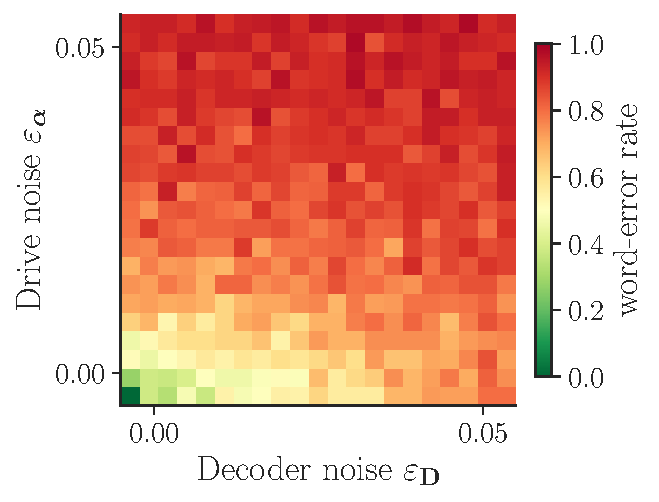
\includegraphics[width=0.6\textwidth]{figures/combined_noise.pdf}
\caption{Combined drive- and decoder-noise robustness scan for the $K=N=3$ symmetric system with the period-11 reference word ($|\mu_2/\mu_1|=0.015$). Multiplicative noise $\varepsilon_{\boldsymbol{\alpha}}$ rescales each drive by $1+\varepsilon_{\boldsymbol{\alpha}}\eta$ ($\eta\sim\mathcal{N}(0,1)$) and likewise per-component for each decoder (then renormalized to unit length). Each cell reports the word-error rate over 25 trials. The dashed iso-contour at 50\% error sits in the $\varepsilon\lesssim 0.02$ region; biologically plausible noise levels ($\varepsilon\sim 0.05$--$0.10$) lie in the saturated upper-right region where the exact firing word is essentially never recovered.}
\label{fig:combined-noise}
\end{figure}


\section{Rate-versus-sequence robustness discussion (main text \S 5)}\label{app:rate-vs-seq}

\paragraph{Robustness of rate versus sequence codes.}
The inverse problem solved here treats the exact firing word $\sigma$ as the quantity to realize, but the analysis of Section~\ref{sec:bifurcation} suggests a more robust encoding may be available. The firing-ratio map $\rho(\boldsymbol{\alpha})$ is a complete devil's staircase on rational rotation numbers \citep[Arnold tongues for analytic circle maps;][]{arnold1961small,herman1979conjugaison}, restated for our family as Theorem~\ref{thm:staircase}, and \emph{within each plateau} the rotation number is exactly invariant under small input perturbations. For $K=2$, Sturmian uniqueness (Remark~\ref{rem:sturmian}) then forces the exact word $\sigma$ to be locked alongside $\rho$, so the rate code and the sequence code coincide on each plateau. For $K\geq 3$ this coincidence breaks: the partition geometry permits several admissible words with the same firing-ratio vector $(\rho_1,\ldots,\rho_K)$, so the word can shift between admissible variants under a perturbation that leaves the rotation number invariant. The robust storage substrate is therefore not the exact spike-by-spike sequence but the \emph{rotation number}, equivalently, the rational plateau the system occupies on the staircase. Under time-varying input the system traces a piecewise-constant trajectory through $\rho$-space, hopping between plateaus, and the temporal code that survives input perturbation is this sequence of plateau visits rather than the underlying spike sequence on each. The inverse problem we solve here treats the exact spike sequence as the quantity to realize and is therefore fragile to input perturbations; the staircase plateaus themselves preserve only the rotation number and are robust at this coarser level. Distinguishing the two experimentally, are sequence-encoding cortical circuits robust at the level of exact spike order or only at the level of population firing ratios?, is a falsifiable prediction the framework offers.


\section{Analytical robustness bound via eigenvector perturbation (main text \S 5)}\label{app:analyt-bound}

\paragraph{Analytical robustness bound.} The tolerance to parameter perturbation can be predicted from eigenvector perturbation theory (the non-symmetric analogue of the Davis--Kahan theorem \citep{davis1970rotation,stewart1990matrix}). For a simple eigenvalue $\mu_1$ of $\vv{M}_\sigma$ with right eigenvector $\vv{u}_1$ and left eigenvector $\vv{w}_1$, a perturbation $\delta\vv{M}$ shifts the eigenvector by
\begin{equation}\label{eq:eigpert}
    \delta\vv{u}_1 = \sum_{k=2}^{N}\frac{\vv{w}_k^\top(\delta\vv{M})\vv{u}_1}{\mu_1-\mu_k}\,\vv{u}_k.
\end{equation}
The denominator $\mu_1-\mu_k$ is the eigenvalue gap: larger gap means smaller perturbation. After dehomogenization, the orbit shift is $\delta\xxi^*=(1/u_N)[\delta\vv{u}_{1:N-1}-\xxi^*\,\delta u_N]$. The orbit survives perturbation $\delta\boldsymbol{\alpha}$ iff $\|\delta\xxi^*\|$ is small enough that the margin remains positive. This yields the tolerance bound
\begin{equation}\label{eq:tolerance}
    \text{tolerance}\;\approx\;\frac{m}{\|\nabla_{\boldsymbol{\alpha}}m\|}\;\propto\;\frac{m\cdot|\mu_1-\mu_2|}{\|\partial\vv{M}_\sigma/\partial\boldsymbol{\alpha}\|\cdot\kappa(\vv{S})},
\end{equation}
where $\kappa(\vv{S})$ is the condition number of the eigenvector matrix. For the RBYGYB orbit, this predicts per-drive tolerances of $0.6$--$19\%$ (tightest on $\alpha_3,\alpha_4$), matching the actual values to within a factor of~2 (Appendix~\ref{app:numerics}). Robustness is thus jointly controlled by the admissibility margin $m$ (geometric) and the eigenvalue gap $|\mu_1-\mu_2|$ (dynamical).

\section{Glossary}\label{sec:glossary}

Throughout, each ``spike'' is an instantaneous Dirac-$\delta$ event in continuous time, and the discrete index $n$ in expressions like $\xxi_n$, $b_n$, or ``step $n$'' counts \emph{spike events} (not equispaced time steps): one $n$-step corresponds to one spike-and-decay segment of continuous time.

\begin{table}[h]
\centering
\small
\renewcommand{\arraystretch}{1.05}
\begin{tabular}{ll}
\hline
Symbol & Meaning \\
\hline
$K,\ N$ & number of neurons; ambient (input) dimension \\
$\DD_i\in\RR^N$ & unit-norm decoder of neuron $i$ \\
$\alpha_i>0$ & suprathreshold drive of neuron $i$ (after change of variables) \\
$\psi_{ij}$ & angle between decoders, $\cos\psi_{ij}=\DD_i^\top\DD_j$ \\
$\yy\in\RR^N$ & readout / population response \\
$\Bsp_i=\{\yy:\DD_i^\top\yy=\alpha_i\}$ & spike bound for neuron $i$ \\
$\vv{U}_i\in\RR^{N\times(N-1)}$ & orthonormal tangent frame of $\Bsp_i$ \\
$\xxi\in\RR^{N-1}$ & tangent coordinate on a bound \\
$\yy^+=\yy+\DD_i$ & post-spike readout after neuron $i$ fires \\
$c_j(\xxi)=\alpha_j/(\DD_j^\top\yy^+)$ & decay factor; next firer maximises $c_j$ \\
$\vv{M}_{j\leftarrow i}\in\RR^{N\times N}$ & per-step transition matrix in homogeneous coordinates \\
$\sigma=(b_0,\ldots,b_{L-1})$ & firing word (sequence of fired neurons) of length $L$ \\
$\vv{M}_\sigma$ & return matrix, $\vv{M}_{b_0\leftarrow b_{L-1}}\cdots\vv{M}_{b_2\leftarrow b_1}\vv{M}_{b_1\leftarrow b_0}$ (right-to-left composition) \\
$\xxi^*$ & dehomogenized dominant eigenvector of $\vv{M}_\sigma$; orbit position on $\Bsp_{b_0}$ \\
$\mu_1,\ldots,\mu_N$ & eigenvalues of $\vv{M}_\sigma$, ordered by decreasing modulus \\
$|\mu_k/\mu_1|$ for $k\geq 2$ & Lyapunov multipliers; orbit stable iff all $<1$ \\
$\rho$ & rotation number / firing ratio of neuron 3 \\
$m(\alpha_2)$ & admissibility margin (continuous score, $>0$ iff $\sigma$ realised) \\
\hline
\end{tabular}
\caption{Notation used throughout. Lower-case bold for vectors, upper-case bold for matrices; calligraphic letters for sets and bounds.}
\label{tab:notation}
\end{table}

\section{Numerical experiment details}\label{app:numerics}
%======================================================================

All experiments were implemented in Python~3.12 using NumPy and SciPy. This appendix specifies every parameter choice needed to reproduce the results.

\subsection{Forward simulation}\label{app:forward-sim}

Every forward simulation uses the same core routine. Starting from an initial tangent coordinate $\xxi_0$ and bound index $b_0$, each step applies the transition map~\eqref{eq:transition-map} by:
\begin{enumerate}[nosep]
    \item Computing the post-spike readout $\yy^+=(\alpha_{b_k}+1)\DD_{b_k}+\vv{U}_{b_k}\xxi_k$.
    \item For each active neuron~$j$ ($\alpha_j>0$), computing the decay factor $c_j=\alpha_j/(\DD_j^\top\yy^+)$.
    \item Selecting $j^*=\arg\max_j c_j$ (subject to $0<c_j\leq 1$).
    \item Landing: $\xxi_{k+1}=\vv{U}_{j^*}^\top(c_{j^*}\yy^+)$.
\end{enumerate}
No ODE solver is needed; the dynamics are exact in discrete time.

\subsection{Figure~\ref{fig:overview-supp}: SCN overview ($N{=}K{=}2$)}\label{app:fig-overview}

Decoder angles $	heta_1=0.25$\,rad, $	heta_2=	heta_1+0.4\pi$\,rad, giving $\psi=0.4\pi$, $\cos\psi\approx 0.309$.

\textbf{Panels (a,b):} Drives $\alpha_1=1.0$, $\alpha_2=0.49$. Orbit found by simulating 5\,000 transient steps from $\xi_0=1.0$ on bound~1, then recording 7~steps. The period-7 word $\sigma=(1,1,2,1,1,1,2)$ and orbit position $\xi^*\approx 0.717$ are verified against the dominant eigenvector of the $2\times 2$ return map $\vv{M}_\sigma$.

\textbf{Panel (c):} First-return map $F_{\!\Bsp_1}:\Bsp_1\to\Bsp_1$, mapping the tangent coordinate $\xi_n$ on bound~1 to the next visit $\xi_{n'}$ on bound~1. Two branches separated by the partition point $\xi_{\mathrm{part}}\approx 0.381$: for $\xi<\xi_{\mathrm{part}}$, the decay factor $c_2>c_1$ so neuron~2 fires next (cross-transition); for $\xi\geq\xi_{\mathrm{part}}$, $c_1>c_2$ so neuron~1 self-fires. Each branch is a M\"obius transformation $\xi\mapsto(a\xi+b)/(c\xi+d)$. The period-7 orbit visits $\Bsp_1$ five times per cycle, so the cobweb converges to a 5-cycle of the first-return map.

\textbf{Panel (d):} Devil's staircase computed by scanning $\alpha_2\in[0.01,\,1.0]$ at $600$ uniformly spaced values. At each value: $5{,}000$ transient steps from four different initial conditions ($\xi_0\in\{0.05,\,0.5,\,1.0,\,1.5\}$), selecting the mixed orbit when found.  Period detection from $300$ recorded steps (requiring $\min(3L,30)$ consecutive matches).  Purple dots mark every distinct plateau with $\rho>0$.

\subsection{Figure~\ref{fig:cobweb_gallery}: Cobweb gallery across the staircase}\label{app:cobweb-gallery}

The cobweb diagram provides a direct visualization of the 
piecewise projective return map as a classical dynamical system on 
the line.  For $K{=}2$, $N{=}2$, the full dynamics reduce to a 
first-return map $F_{\!\Bsp_1}:\Bsp_1\to\Bsp_1$ with two branches, each a
M\"obius transformation:
\begin{itemize}[nosep]
\item \emph{Cross branch} ($\xi<\xi_{\mathrm{part}}$): $c_2>c_1$, 
so neuron~2 fires next.  The readout visits $\Bsp_2$ before returning 
to $\Bsp_1$, giving $F(\xi)=\alpha_1 \cdot
[(\alpha_2+1)\vv{w}_{01}+\vv{R}_{01}\,\alpha_2\,\{(\alpha_1+1)\vv{w}_{10}+\vv{R}_{10}\xi\}/
\{(\alpha_1+1)\cos\psi_{21}+\vv{v}_{10}\xi\}] / [\cdots]$ (composition of two
transition maps).
\item \emph{Self branch} ($\xi\geq\xi_{\mathrm{part}}$): $c_1>c_2$, 
so neuron~1 self-fires.  The map is simply 
$F(\xi)=\alpha_1\xi/(\alpha_1+1)$, a uniform contraction toward the 
foot $\xi=0$.
\end{itemize}
The partition point $\xi_{\mathrm{part}}$ is the unique $\xi$ where 
$c_1=c_2$, i.e.\ $\alpha_1/(\alpha_1+1)=\alpha_2/\{(\alpha_1+1)\cos\psi_{21}+\vv{v}_{10}\xi\}$.  
As $\alpha_2$ increases, $\xi_{\mathrm{part}}$ decreases (the cross 
region grows), and the orbit visits $\Bsp_2$ more frequently, 
increasing~$\rho$.

Figure~\ref{fig:cobweb_gallery} shows the first-return map and cobweb 
at eight values of $\alpha_2$, one per distinct mode-locked plateau.  
The key observations are:
\begin{enumerate}[nosep]
\item At $\alpha_2=0.20$ (below threshold), only the self branch 
exists: $F(\xi)=0.5\xi$, converging to the fixed point $\xi^*=0$ 
(period-1 self-trap, $\rho=0$).
\item At $\alpha_2=0.335$ ($\rho=1/6$), the cross branch has appeared 
and the cobweb traces a 5-cycle on $\Bsp_1$ (five of six orbit steps 
land on~$\Bsp_1$).
\item At $\alpha_2=0.60$ ($\rho=1/3$, the widest mixed plateau at 
width~$0.10$), the cobweb traces a 2-cycle: each visit to $\Bsp_1$ 
alternates between a self-transition and a cross-transition.
\item At $\alpha_2=0.80$ ($\rho=3/7$), the cobweb traces a 4-cycle 
with three cross-transitions per period.
\end{enumerate}
In every case, the cobweb converges to a periodic cycle (never a fixed 
point, except at $\rho=0$), confirming that the first-return map is a
degree-$1$ piecewise-M\"obius map with a unique stable periodic orbit at each
rational rotation number.

\begin{figure}[t]
\centering
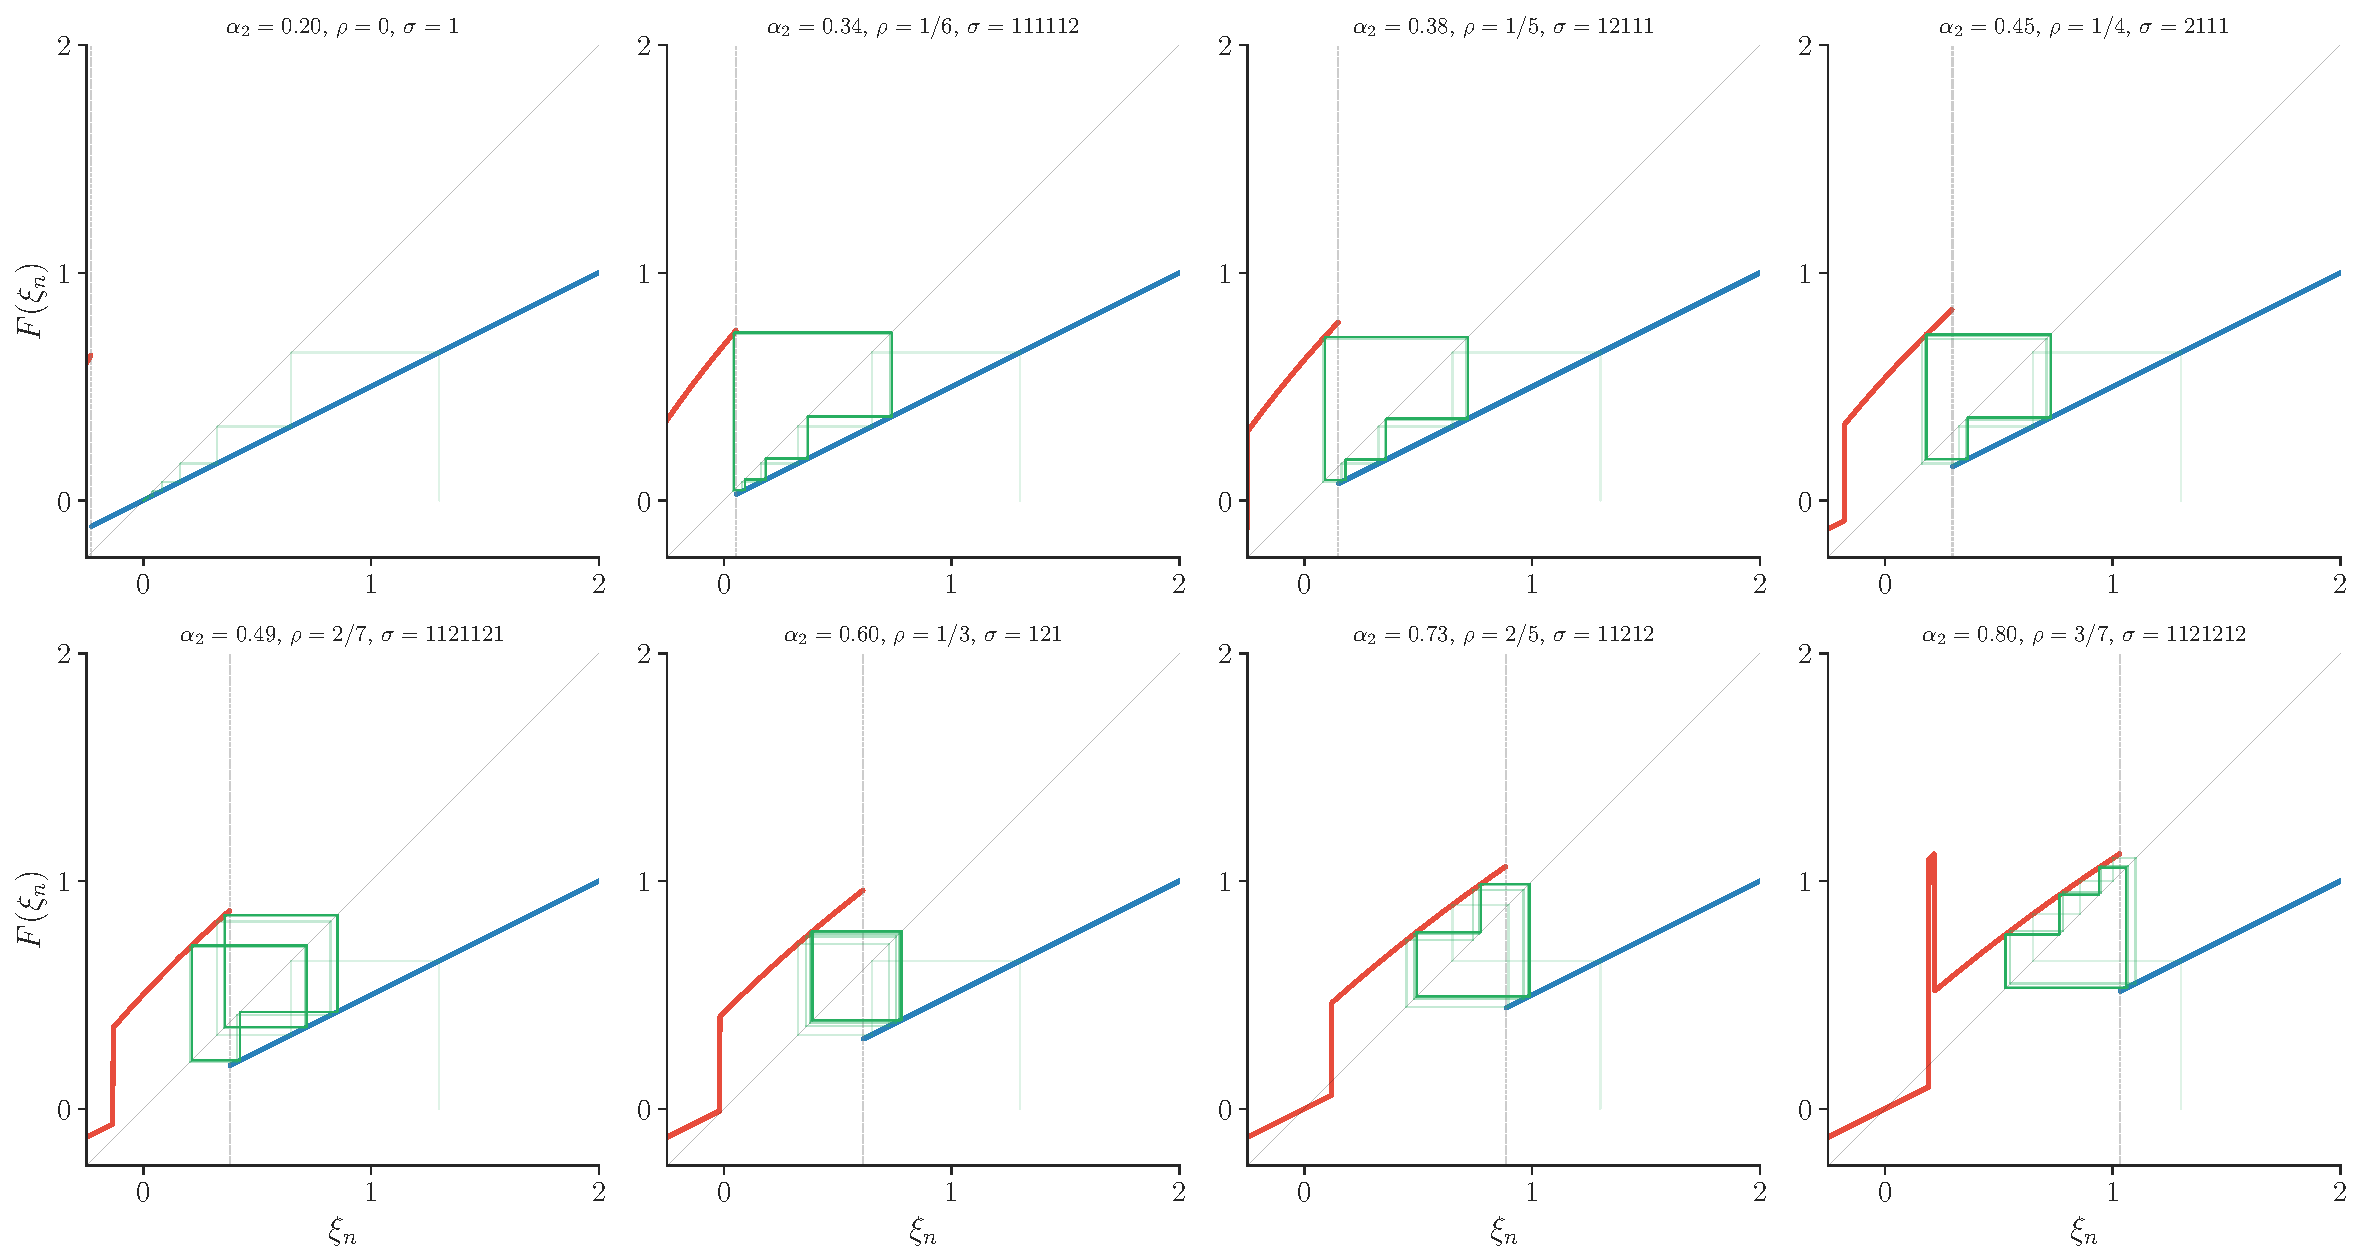
\includegraphics[width=\textwidth]{figures/cobweb_gallery.pdf}
\caption{Cobweb diagrams of the first-return map $F_{\!\Bsp_1}:\Bsp_1\to\Bsp_1$ at eight values of $\alpha_2$, one per distinct mode-locked plateau of the devil's staircase.  Red: cross-transition branch ($\xi<\xi_{\mathrm{part}}$); blue: self-transition branch ($\xi\geq\xi_{\mathrm{part}}$); dashed: partition point.  Green cobwebs (from $\xi_0=1.3$) converge to the unique stable cycle, whose period on~$\Bsp_2$ equals the number of~1's in the firing word~$\sigma$.}
\label{fig:cobweb_gallery}
\end{figure}

\subsection{Staircase orbit examples ($K{=}N{=}2$)}\label{app:staircase-examples}

Figures~\ref{fig:staircase1}--\ref{fig:staircase8} show all 48 
distinct mode-locked orbits found in the devil's staircase scan of 
Figure~\ref{fig:overview-supp}d, organized into eight pages of six panels 
each.  Each panel displays the orbit in $\RR^2$ at a single 
$\alpha_2$ value (with $\alpha_1=1.0$, $\psi=0.4\pi$ throughout):
\begin{itemize}[nosep]
\item \emph{Top row:} Eigenvector-predicted orbit positions (colored 
dots from the dominant eigenvector of $\vv{M}_\sigma$), with spike 
(colored) and decay (gray dashed) connections.
\item \emph{Bottom row:} Simulation from a random initial condition, 
converging to the same positions.
\end{itemize}
In every case, theory and simulation match to machine precision.  
The orbits span firing ratios from $\rho_{\text{spike}}=1/8$ (period~8, one
neuron-1 firing per cycle) to $\rho_{\text{spike}}=4/9$ (period~9, nearly equal
firing rates).  The firing words are all Sturmian 
(Remark~3): for any two subwords of the same length, the 
neuron-1 count differs by at most~1.

\begin{figure}[p]
\centering
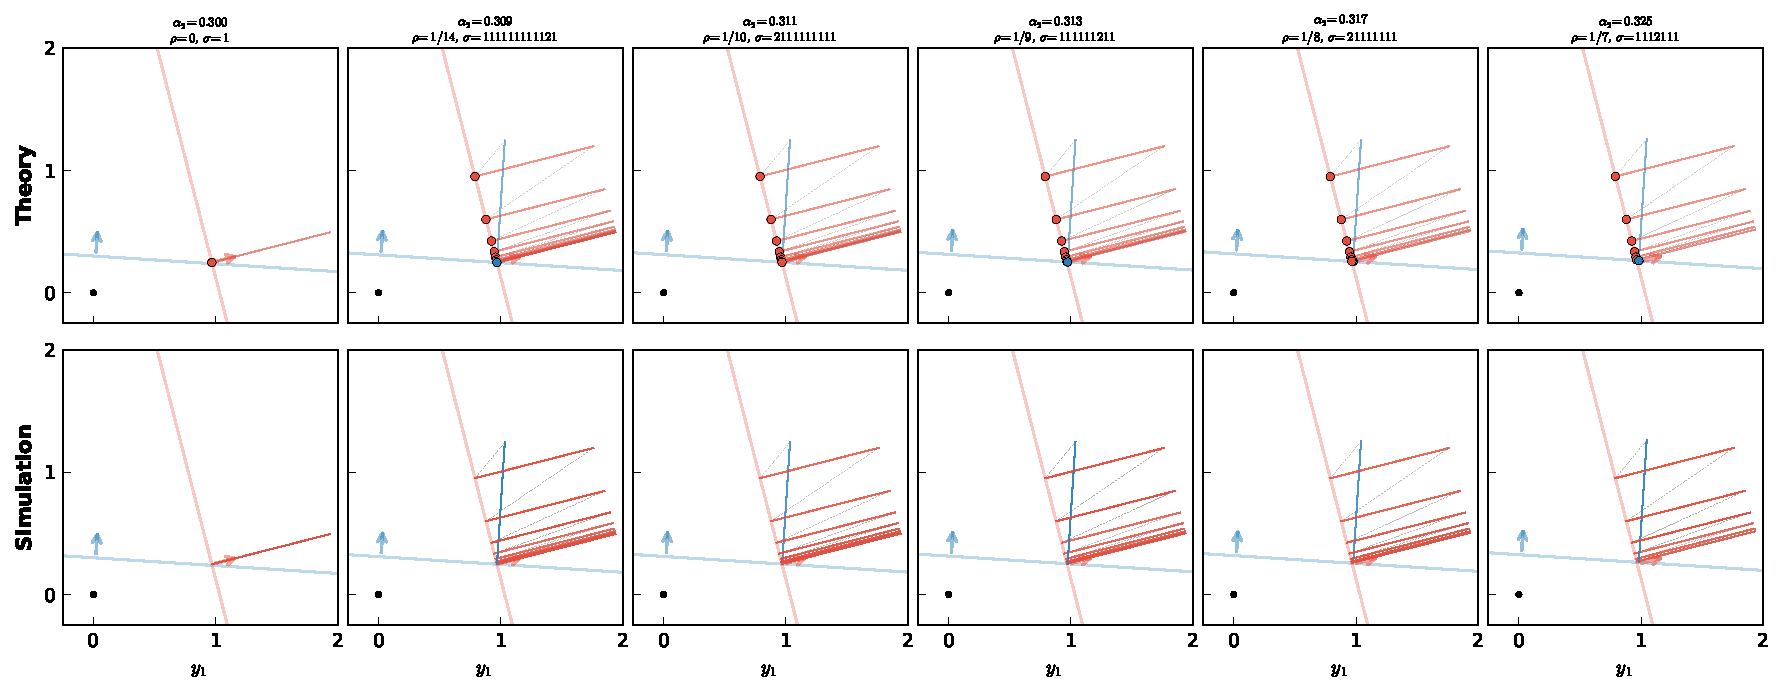
\includegraphics[width=\textwidth]{figures/staircase_examples_1.pdf}
\caption{Staircase orbit examples, page 1 of 8.}
\label{fig:staircase1}
\end{figure}

\begin{figure}[p]
\centering
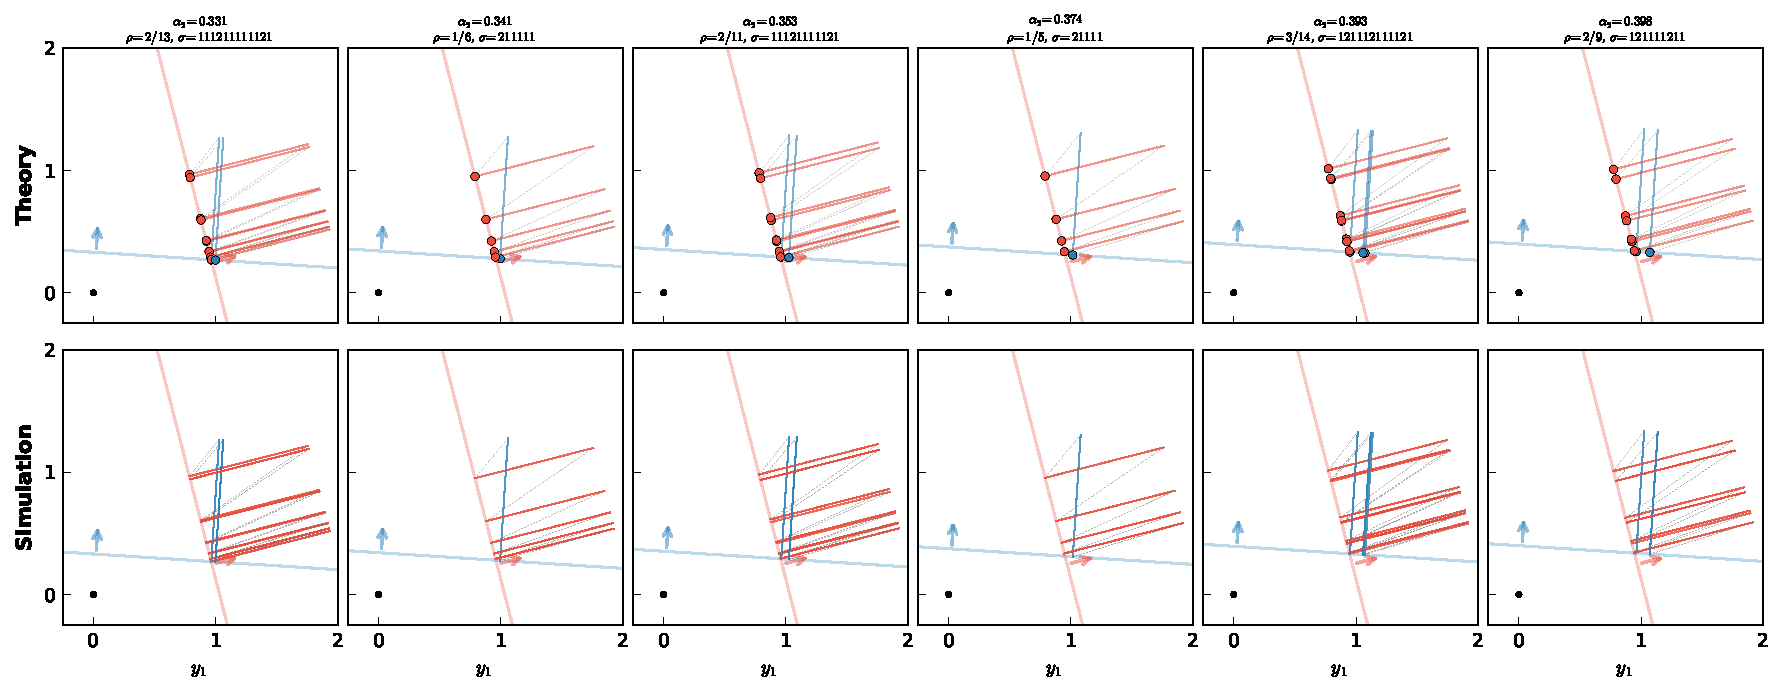
\includegraphics[width=\textwidth]{figures/staircase_examples_2.pdf}
\caption{Staircase orbit examples, page 2 of 8.}
\label{fig:staircase2}
\end{figure}

\begin{figure}[p]
\centering
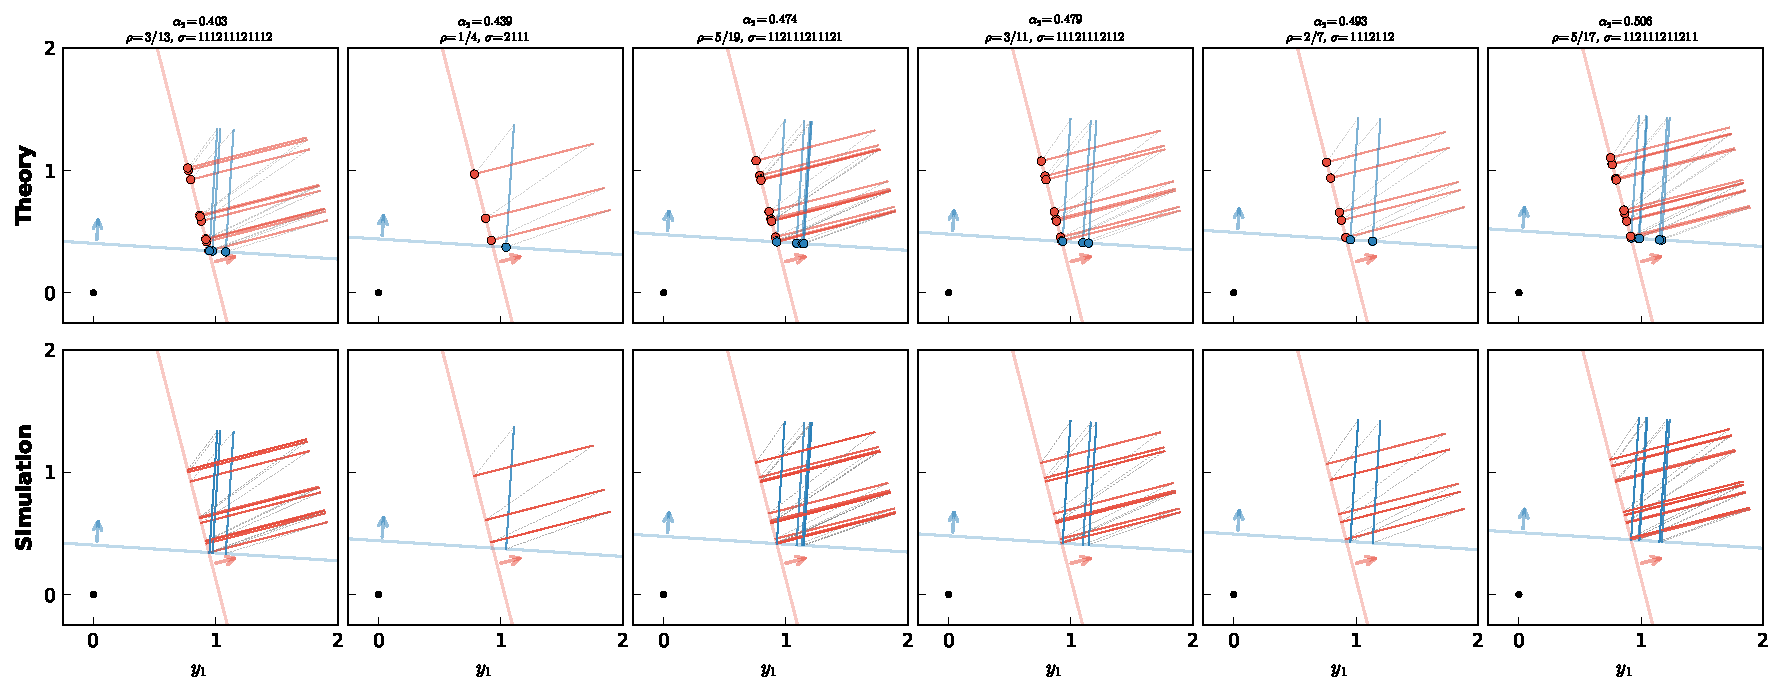
\includegraphics[width=\textwidth]{figures/staircase_examples_3.pdf}
\caption{Staircase orbit examples, page 3 of 8.}
\label{fig:staircase3}
\end{figure}

\begin{figure}[p]
\centering
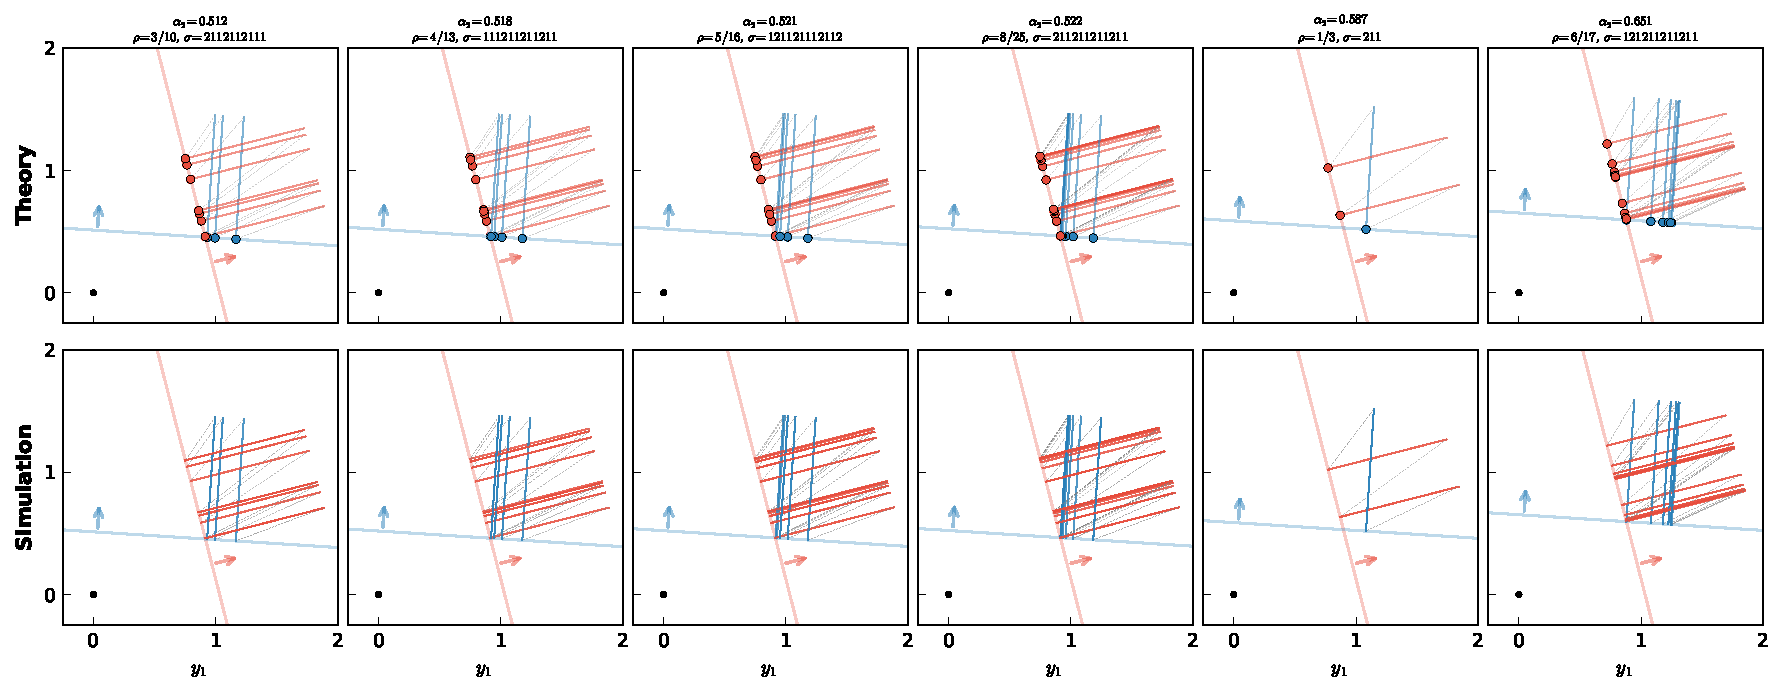
\includegraphics[width=\textwidth]{figures/staircase_examples_4.pdf}
\caption{Staircase orbit examples, page 4 of 8.}
\label{fig:staircase4}
\end{figure}

\begin{figure}[p]
\centering
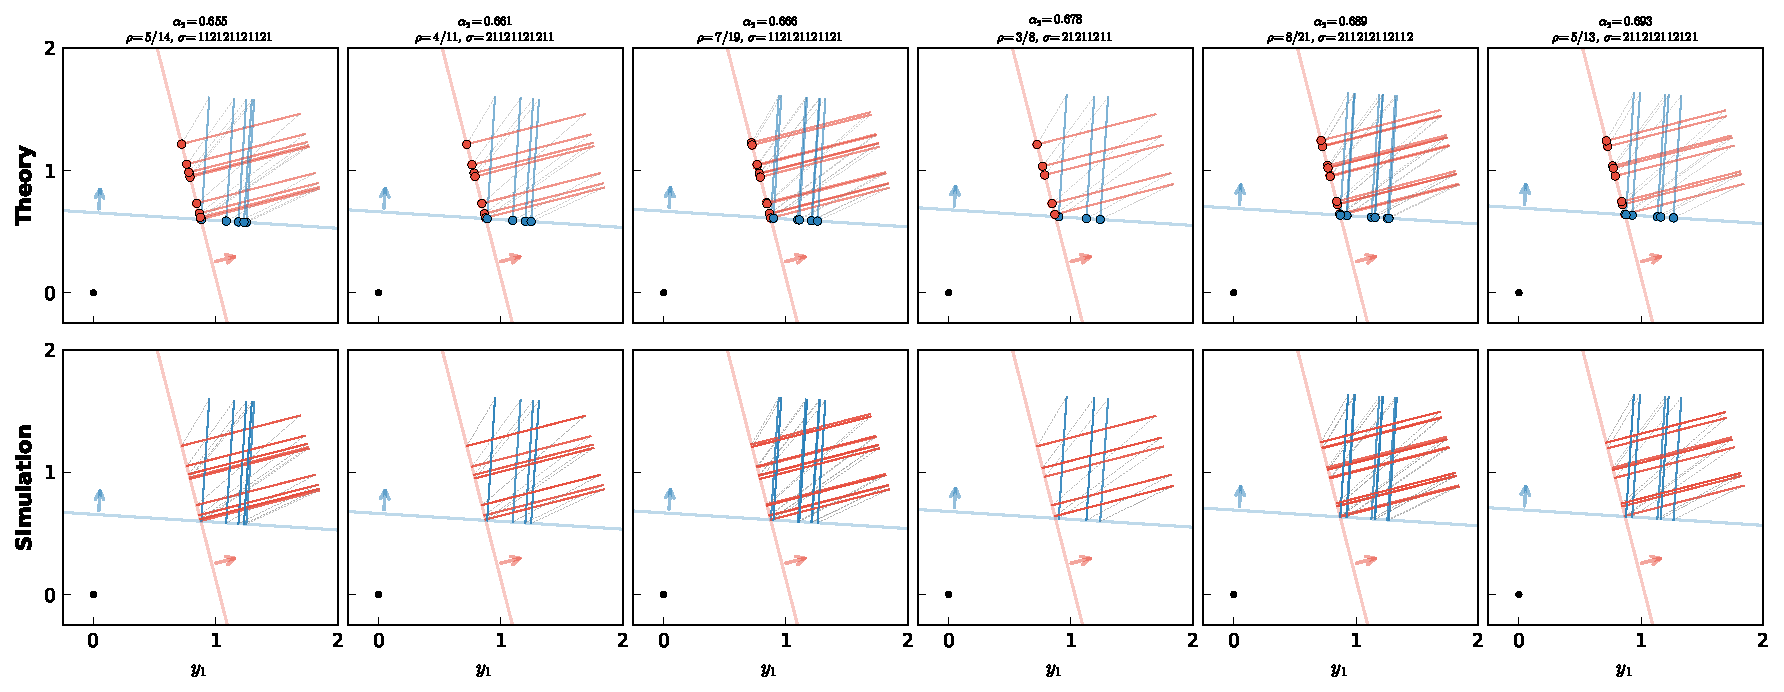
\includegraphics[width=\textwidth]{figures/staircase_examples_5.pdf}
\caption{Staircase orbit examples, page 5 of 8.}
\label{fig:staircase5}
\end{figure}

\begin{figure}[p]
\centering
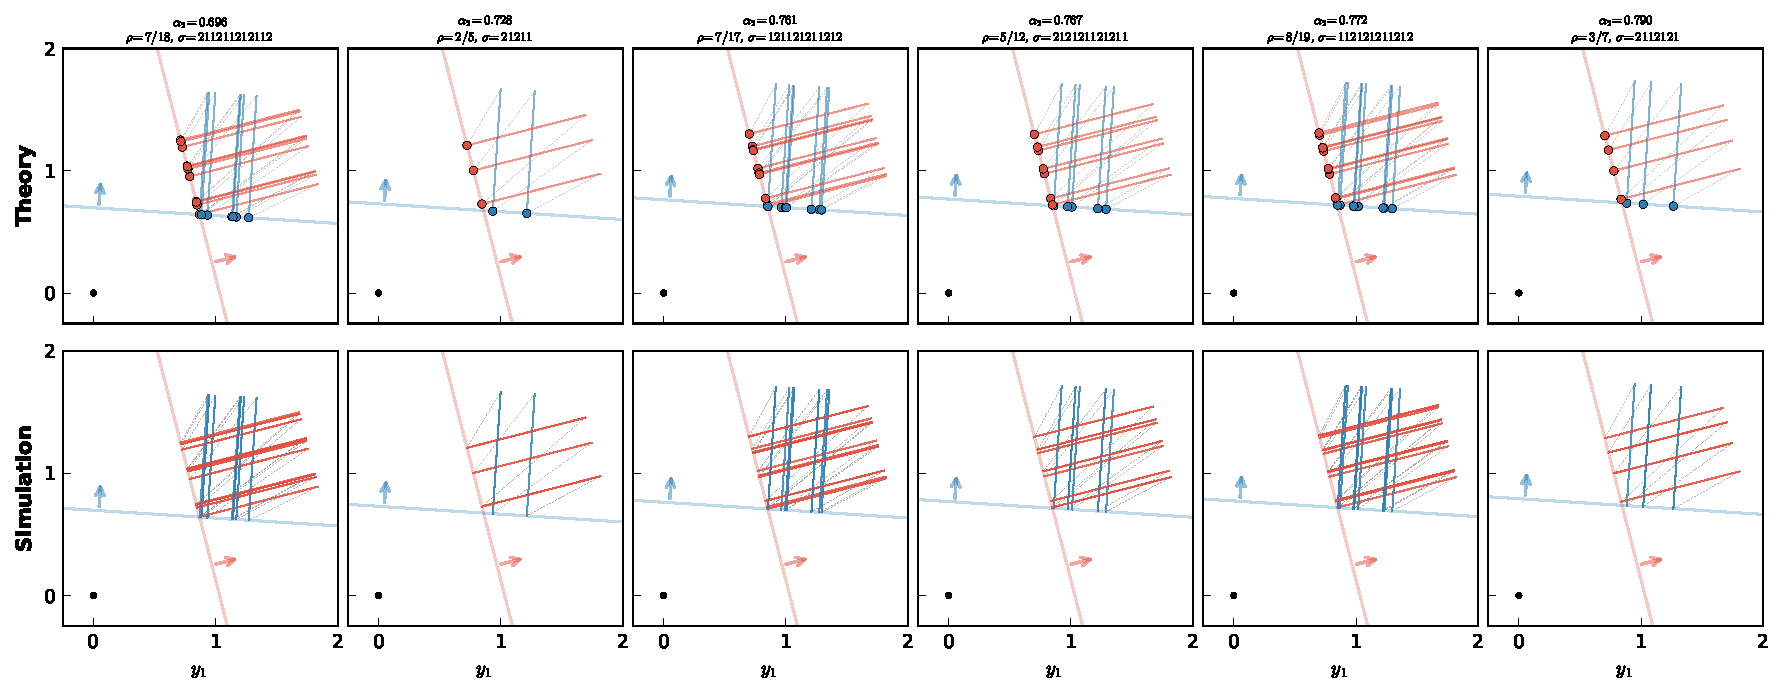
\includegraphics[width=\textwidth]{figures/staircase_examples_6.pdf}
\caption{Staircase orbit examples, page 6 of 8.}
\label{fig:staircase6}
\end{figure}

\begin{figure}[p]
\centering
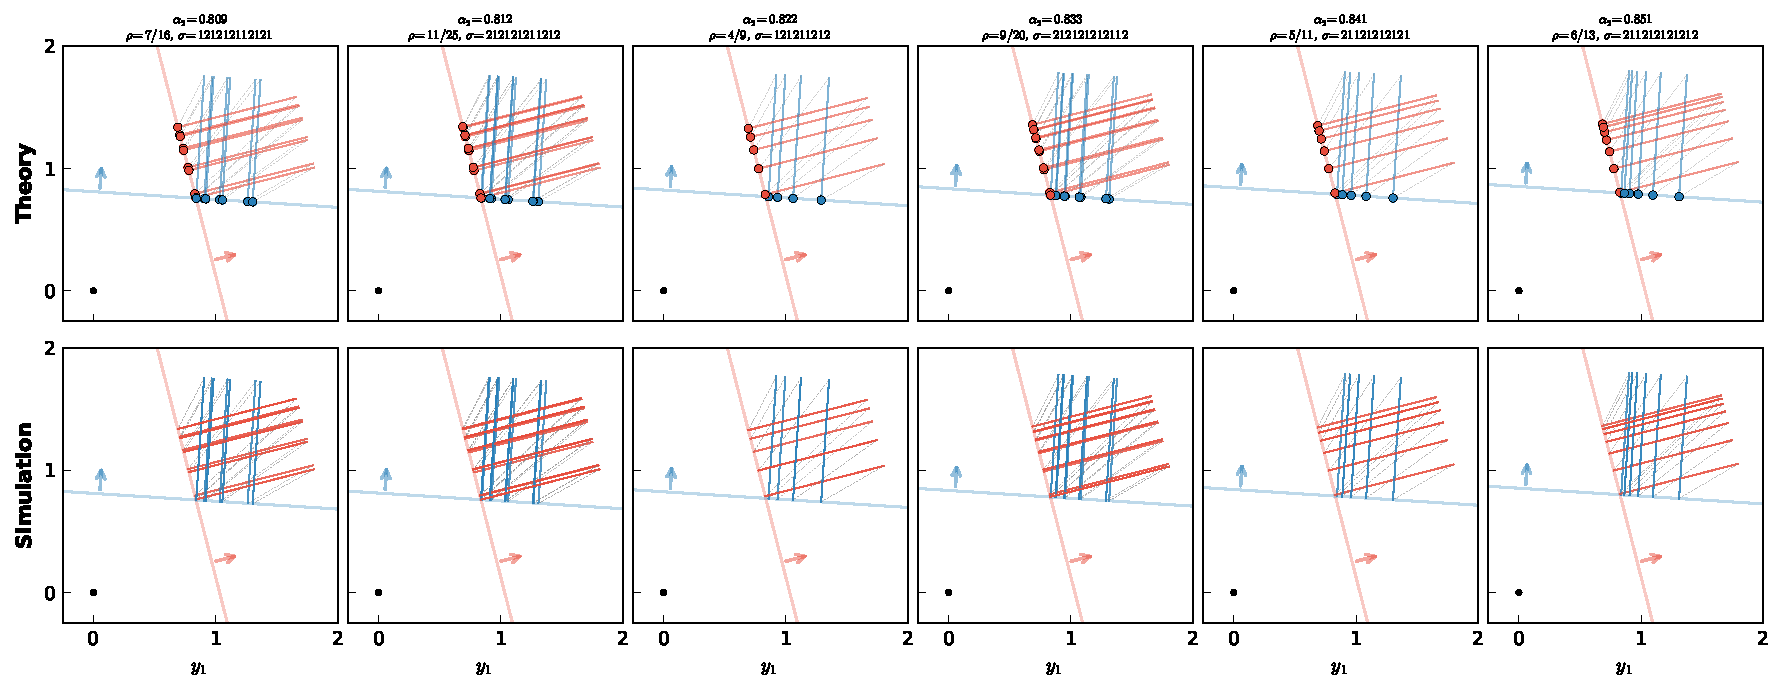
\includegraphics[width=\textwidth]{figures/staircase_examples_7.pdf}
\caption{Staircase orbit examples, page 7 of 8.}
\label{fig:staircase7}
\end{figure}

\begin{figure}[p]
\centering
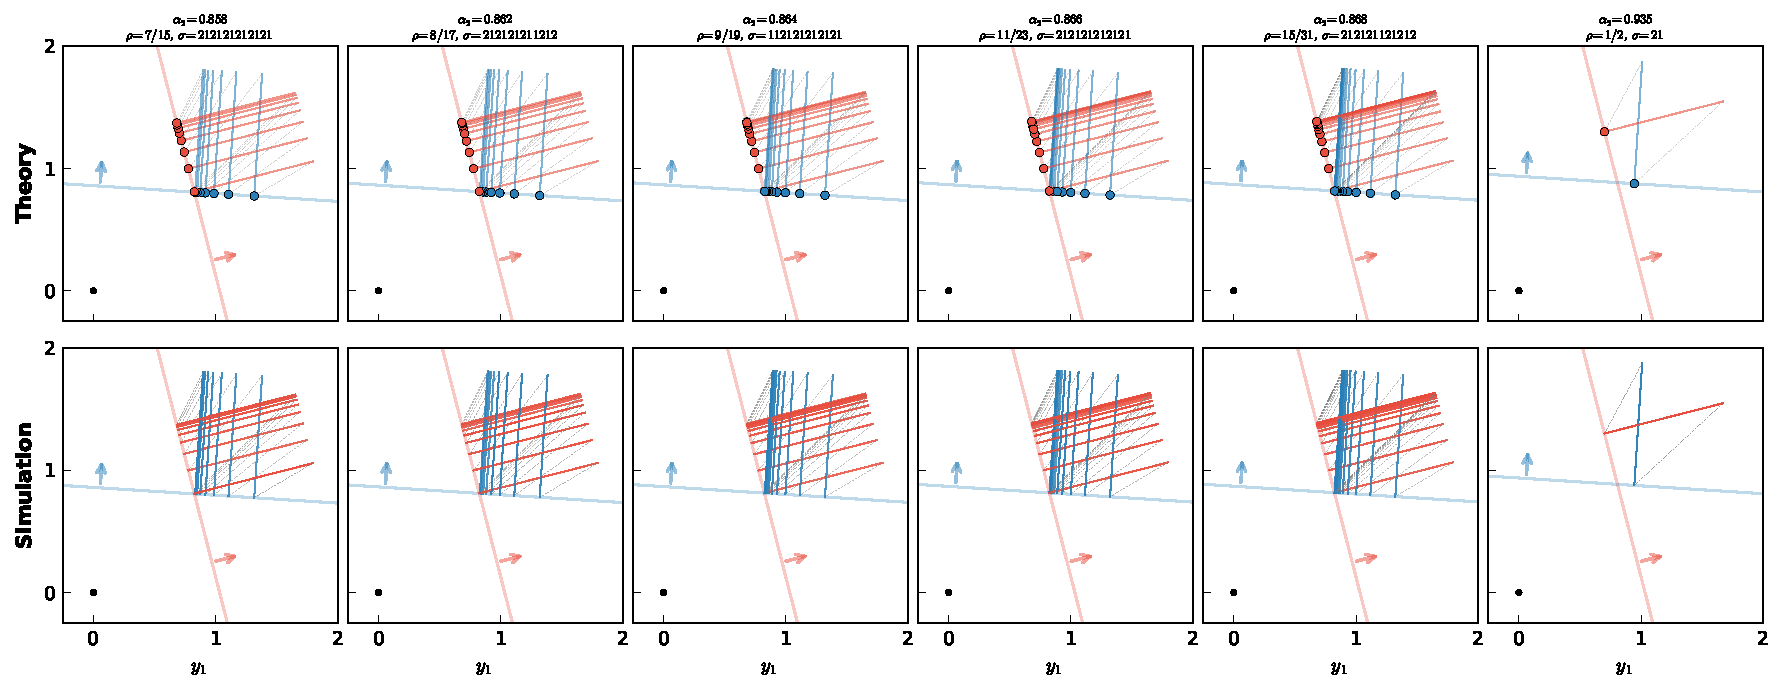
\includegraphics[width=\textwidth]{figures/staircase_examples_8.pdf}
\caption{Staircase orbit examples, page 8 of 8.}
\label{fig:staircase8}
\end{figure}

\subsection{Figure~\ref{fig:chaos}: Order-chaos transition ($K{=}4$, $N{=}3$)}\label{app:fig-chaos}

\textbf{Chaotic system:} Decoders (each unit-normalized) and drives:
\begin{align*}
\DD_1 &\approx (0.566,\,-0.791,\,-0.233), & \DD_2 &\approx (0.748,\,-0.260,\,0.611), \\
\DD_3 &\approx (-0.296,\,-0.526,\,-0.798), & \DD_4 &\approx (0.694,\,-0.601,\,0.395), \\
\boldsymbol{\alpha} &\approx (0.966,\,0.342,\,0.487,\,0.653). & &
\end{align*}
Pairwise cosines include the minimum $\cos\psi_{23}\approx -0.57$ (and $\cos\psi_{34}\approx -0.20$).

\textbf{Panel (a): phase diagram.} 800~random $(\vv{D},\boldsymbol{\alpha})$ configurations with $K=4$, $N=3$. Decoders: rows of a $4\times 3$ standard normal matrix, unit-normalized. Drives: i.i.d.\ $\text{Exp}(0.8)$. Random seed~42. Per sample: 1\,500~transient steps + 3\,000~recording steps. Classification: $\lambda_{\max}>0$ = chaotic ($5$ cases out of $800$, including one weakly chaotic case with $\lambda_{\max}\approx 0.004$), all with $\min_{i<j}\cos\psi_{ij}<-0.5$. The accent-blue open square marks the specific chaotic configuration used in panels~(b) and~(c) (constructed to prove chaos; not one of the 800 random samples).

\textbf{Panel (b): sensitivity to initial conditions.} After a $10\,000$-step transient off a random seed on bound~$\Bsp_1$, we pre-record $400\cdot 12+1=4801$ consecutive steps of the converged chaotic orbit. Each of $400$ perturbation pairs is anchored at a different point along that trajectory (spacing $12$ steps between successive anchors), perturbed by $\varepsilon=10^{-12}$ in a random unit tangent direction (seed~0). Each pair is tracked for $150$~steps; median and inter-quartile range of the ambient-space distance $\|\yy^{\mathrm{ref}}_t-\yy^{\mathrm{pert}}_t\|$ are plotted on a log scale. The dashed reference line is $\varepsilon\cdot e^{\lambda_{\max}t}$ with $\lambda_{\max}$ set to the QR-measured value from the Lyapunov calculation below.

\textbf{Lyapunov spectrum.} We report two consistent measurements. \emph{(1)~Twin-trajectory:} after $5\,000$~transient steps, initialize a twin at $\varepsilon=10^{-9}$; at each step record $\ln(\|\delta\xxi\|/\varepsilon)$ and renormalize. Converges to $\lambda_{\max}=0.282\pm 0.002$ over $20\,000$~steps. \emph{(2)~QR accumulation of a $2\times 2$ per-step Jacobian:} the accompanying code (\texttt{code/fig\_chaos.py}) uses a central finite difference with step size $10^{-6}$, one-sided on the branch flip fallback; a symbolic analytic Jacobian is derivable in closed form from the transition map~\eqref{eq:transition-map} as $\vv{J}(\xxi)=(1/\delta)(\alpha_j\vv{R}_{ji}-\xxi'\vv{v}_{ji}^\top)$ (see the proof of Theorem~\ref{thm:cone}(b)). Accumulation is by QR every step over $50$~segments of $1000$~steps after a $10\,000$-step transient. Result: $\lambda_1=0.288$, $\lambda_2=-0.388$ nats/step (agreement with the paper-cited $\lambda_1=0.285\pm 0.010$, $\lambda_2=-0.389\pm 0.008$ from the analytic-Jacobian run), with all $50$ segments giving $\lambda_1>0.26$.

\textbf{Panel (c): strange attractor.} $50\,000$~iterates from the converged state; the ${\sim}20\,000$ visits to $\Bsp_3$ (the most frequently visited bound) are plotted in the tangent chart $(\xi_1,\xi_2)$.

\subsection{Figure~\ref{fig:simon}: Sequence working memory ($K{=}4$, $N{=}3$)}\label{app:fig-simon}

\textbf{Decoders:} Four unit vectors arranged symmetrically around the $(1,1,1)/\sqrt{3}$ axis:
$\DD_i = (1,1,1)/\sqrt{3} + 0.6[\cos(i\pi/2)\,\vv{u}_1+\sin(i\pi/2)\,\vv{u}_2]$,
where $\vv{u}_1=(1,-1,0)/\sqrt{2}$, $\vv{u}_2=\vv{u}_1\times(1,1,1)/\sqrt{3}$, for $i=0,1,2,3$, each unit-normalized. All pairwise cosines are positive ($\cos\psi\approx 0.47$).

\textbf{Panel (b):} Drives $\boldsymbol{\alpha}=(2.02,\,2.05,\,2.43,\,2.35)$, producing the period-6 word $\sigma=\text{RBYGYB}=(1,3,4,2,4,3)$. Orbit positions from the dominant eigenvector of the $3\times 3$ return map $\vv{M}_\sigma$. Transient trajectory: 48~steps from $\xxi_0=(0,0)$ on bound~1.

\textbf{Panel (c), noise robustness:} 30~log-spaced noise levels $\eta_{\text{std}}\in[10^{-3.5},\,10^{-0.3}]$. At each level, 30~independent trials (seeds 0--29). Each trial: 200~noiseless transient steps to converge, then 600~noisy steps. Noise model: S1-type additive Gaussian $\boldsymbol{\eta}\sim\mathcal{N}(\vv{0},\eta_{\text{std}}^2\vv{I}_3)$ added to the post-spike readout $\yy^+$ before decay. Word error rate = (number of steps where $b_k\neq\sigma_{k\bmod L}$)/(total steps). Admissibility margin for this orbit: $m\approx 0.005$.

\subsection{Figure~\ref{fig:3d}: Three-neuron example ($K{=}N{=}3$)}\label{app:fig-3d}

Three decoders in $\RR^3$ arranged symmetrically about the axis
$[1,1,1]^\top/\sqrt{3}$ with pairwise cosines
$\cos\psi_{ij}=0.507$ for all pairs.  Drives
$\boldsymbol{\alpha}=(1.0,\,0.9,\,0.7)$.

\textbf{Panel~(a).}
Geometry rendered at elevation $70^\circ$, azimuth $180^\circ$.
Each bound $\Bsp_i$ is shown as a filled rectangle in the plane
$\DD_i^\top\yy=\alpha_i$, sized to cover the orbit points and
the foot $\alpha_i\DD_i$.  The $11$ colored dots are the
eigenvector-predicted orbit positions; spike (colored) and decay
(gray dashed) segments connect consecutive points.

\textbf{Panel~(b).}
Converged firing pattern over two full periods ($22$~steps), started
from the eigenvector $\xxi^*$.  Each trace shows
$\DD_j^\top\yy$ for $j=0,1,2$; dots mark which neuron fires.
Dashed horizontal lines indicate the thresholds $\alpha_j$.

\textbf{Panel~(c).}
Convergence to the limit cycle from $500$ random initial conditions
($\xxi_0\sim\mathcal{N}(\mathbf{0},\,1.5^2\vv{I})$, $b_0$ uniform on
$\{0,1,2\}$).  At each step~$n$, the distance to the limit cycle is
$\min_{k:\,b_k=b_{\text{sim}}} \|\xxi_{\text{sim}}-\xxi_k^*\|$,
i.e.\ the minimum over all theory points on the same bound
(accounting for phase).  Of the $500$ trials, $448$ ($90\%$) converge
to the period-11 orbit; the remaining $52$ ($10\%$) self-trap on
$\Bsp_3$.  Statistics are computed over the converging subset only.
The dashed line shows the theoretical envelope
$C\,|\mu_2/\mu_1|^{n/L}$ with $|\mu_2/\mu_1|=0.015$.

\textbf{Panel~(d).}
All three firing ratios $\rho_0,\rho_1,\rho_2$ as $\alpha_3$ varies
over $[0.6,\,1.4]$ (fixed $\alpha_1=1.0$, $\alpha_2=0.9$).  At each
of $200$ parameter values, $10$~random initial conditions are
simulated for $2{,}000$ transient steps.  Distinct orbits are
identified by their $(\rho_0,\rho_1,\rho_2)$ tuple (collapsing cyclic
permutations).  Colored dots: mixed orbits visiting $\geq 2$ bounds.
$\times$~markers: self-trapping orbits ($\rho_j=1$ for a single
neuron).  Stars mark the working point $\boldsymbol{\alpha}=(1.0,0.9,0.7)$.

\subsection{Figure~\ref{fig:3d_staircases}: Three-neuron staircases across drives}\label{app:fig-3d-staircases}

Same decoder geometry as Figure~\ref{fig:3d}.  Each panel scans one
drive $\alpha_i\in[0.4,\,1.5]$ at $300$ values while holding the other
two fixed at the working point.  All three firing ratios are plotted
simultaneously; stars mark the common working point
$\boldsymbol{\alpha}=(1.0,0.9,0.7)$.

\subsection{Higher-dimensional verification}\label{app:highd}

We verify the eigenvector orbit prediction across $13$ configurations
spanning the square ($K{=}N$), underdetermined ($K{<}N$), and
overdetermined ($K{>}N$) regimes (Table~\ref{tab:highd}).

\paragraph{Decoder construction.}
For each $(K,N)$, we generate $K$ decoders in $\RR^N$ by drawing
random vectors with strictly positive components and normalizing,
guaranteeing $\cos\psi_{ij}>0$ for all pairs.  Drives are drawn
uniformly from $[0.4,\,1.0]$.

\paragraph{Procedure.}
At each configuration: (i)~simulate $10{,}000$ transient steps;
(ii)~detect the period~$L$ from $500$ recorded steps;
(iii)~compose the $L$ transition matrices into
$\vv{M}_\sigma\in\RR^{N\times N}$;
(iv)~extract the dominant eigenvector and unfold the full orbit;
(v)~compare to the simulation orbit with phase alignment (testing all
$L$ cyclic offsets).

\paragraph{Key observations.}
The return map size is $N{\times}N$ regardless of~$K$: for $K=50$
neurons in $N=10$ dimensions, $\vv{M}_\sigma$ is $10{\times}10$.
In the overdetermined regime ($K>N$), at most $O(N)$ neurons
participate because the $(N{-}1)$-dimensional tangent space has
$O(N)$ partition regions.  In the underdetermined regime ($K<N$),
stability requires all $N{-}1$ eigenvalue ratios to satisfy
$|\mu_k/\mu_1|<1$; the extra ratios correspond to spectator
directions not directly excited by the orbit.

\paragraph{Numerical considerations.}
For large $N$, the dominant eigenvalue $|\mu_1|$ grows exponentially
with $L$.  For $L\gtrsim 100$ and $N\gtrsim 50$, the matrix product
may require periodic rescaling to avoid overflow; all results reported
here used standard double precision without encountering this issue.

\subsection{Noise taxonomy (S-type and D-type)}\label{app:noise}

\textbf{S-type (state) noise:} Applied independently at each spike step.
\begin{itemize}[nosep]
    \item \emph{S1 (readout noise):} $\yy^+\mapsto\yy^++\boldsymbol{\eta}$, $\boldsymbol{\eta}\sim\mathcal{N}(\vv{0},\eta_{\text{std}}^2\vv{I}_N)$.
    \item \emph{S2 (tangent noise):} $\xxi\mapsto\xxi+\boldsymbol{\eta}$, $\boldsymbol{\eta}\sim\mathcal{N}(\vv{0},\eta_{\text{std}}^2\vv{I}_{N-1})$.
    \item \emph{S3 (timing jitter):} decay factor $c_j\mapsto c_j\cdot e^{\eta_{\text{std}} z}$, $z\sim\mathcal{N}(0,1)$.
\end{itemize}
Threshold for zero word errors: $\eta_{\text{std}}\lesssim 0.005$ (S1, S2), $\eta_{\text{std}}\lesssim 0.001$ (S3). S3 is most disruptive because it directly scrambles the partition (which neuron fires next).

\textbf{D-type (dynamical) noise:} Persistent parameter perturbation, fixed per trial.
\begin{itemize}[nosep]
    \item \emph{D1 (heterogeneous leaks):} $\lambda_i=\exp(\eta_{\text{std}} z_i)$, $z_i\sim\mathcal{N}(0,1)$. Decay becomes $\yy(\tau)=\mathrm{diag}(e^{-\lambda_i\tau})\yy^+$; first bound hit found via root-finding (SciPy \texttt{brentq}).
    \item \emph{D2 (noisy drives):} $\alpha_i\mapsto\alpha_i+\eta_{\text{std}} z_i$, clamped to $\alpha_i\geq 0.1$.
    \item \emph{D3 (finite spike width):} Spike is an exponential pulse of duration $\delta$: $\yy^+=e^{-\lambda\delta}\yy_{\text{on}}+(1-e^{-\lambda\delta})\DD_i$. For $\delta\to 0$, recovers the instantaneous spike. The orbit persists even at $\delta=1$ because the finite pulse rescales the effective drive without changing the word.
    \item \emph{D4 (noisy decoders):} $\DD_i\mapsto(\DD_i+\eta_{\text{std}}\boldsymbol{\eta}_i)/\|\DD_i+\eta_{\text{std}}\boldsymbol{\eta}_i\|$, with recomputed tangent frames.
\end{itemize}
All D-type perturbations: word survives at $\eta_{\text{std}}\leq 0.01$, breaks at $\eta_{\text{std}}\geq 0.03$--$0.05$.

\subsection{Input-driven word switching}\label{app:input-switch}

\textbf{Setup:} Fix $\vv{D}$ and $\vv{T}$ such that $\boldsymbol{\alpha}=\vv{D}^\top\xx_0-\vv{T}=(2.02,\,2.05,\,2.43,\,2.35)$ for $\xx_0\approx(1.09,\,1.65,\,1.73)$. Then vary $\xx=\xx_0+s\cdot\hat{\vv{v}}$ for 16 unit directions $\hat{\vv{v}}$ and 6 magnitudes $s\in\{0.1,0.2,0.5,1.0,1.5,2.0\}$.

\textbf{Results:} 62 unique periodic firing words produced by the same network under different inputs. Small perturbations ($s\leq 0.1$) yield cyclic extensions of the original word; large perturbations ($s\geq 1$) produce qualitatively different sequences. The input $\xx$ navigates the devil's staircase in the $K$-dimensional drive space, selecting different mode-locked plateaus.

\subsection{Inverse problem: margin optimization}\label{app:inverse}

\textbf{Figure~\ref{fig:inverse} (panels a--c): Margin landscape.}
For $K{=}N{=}2$ with $\psi=0.4\pi$, the margin 
$m(\alpha_1,\alpha_2)$ is computed on a $150{\times}150$ grid over 
$\alpha_i\in[0.1,\,2.5]$.  At each grid point: the return map 
$\vv{M}_\sigma$ is assembled, its dominant eigenvector extracted, the 
full orbit unfolded, and the margin evaluated as the minimum gap 
$c_{j^*}-c_j$ across all $L$~steps and all competing neurons~$j$.  
Points where the eigenvector is degenerate or the orbit self-intersects 
a partition boundary are marked inadmissible ($m<0$).  The 
zero-margin contour ($m=0$, black line) delineates the admissible 
region.  The star marks the maximum-margin configuration, found by 
exhaustive grid search.

The shrinking of the admissible region with word length is visible: 
$\sigma=(1,2)$ has a broad admissible region (panel~a), while 
$\sigma=(1,1,2,1,1,1,2)$ has a thin sliver (panel~c, 
$m_{\max}=0.02$).  This illustrates the fundamental capacity 
constraint: longer words require more precisely tuned drives.

\textbf{Objective:} The admissibility margin $m(\boldsymbol{\alpha})$, defined as the minimum gap between the target and competing decay factors across all $L$~steps of the orbit. For each candidate $\boldsymbol{\alpha}$: compute the return map $\vv{M}_\sigma$, find its dominant eigenvector (NumPy \texttt{eig}), extract the orbit, and evaluate $m$.

\textbf{Optimizer:} SciPy \texttt{differential\_evolution} with population size~15, maximum 300~iterations, tolerance $10^{-5}$, bounds $\alpha_i\in[e^{-1.5},\,e^{2.5}]$ (search in log-space). Followed by SciPy \texttt{minimize} (Nelder--Mead, 200~iterations) for local polishing. Random seed~42.

\textbf{Results (Table~1):} All words with $K\leq 3$, $N=3$ successfully solved (positive margin). Computation time: 0.2--2\,s per word on a single CPU core.

\subsection{Exact inverse from prescribed orbit}\label{app:exact-inverse}

\textbf{Formulation:} $L(N{-}1)$ bilinear equations in $K$~unknowns. For each step $k$, the orbit consistency condition $\alpha_{b_{k+1}}(\DD_{b_{k+1}}^\top\yy_k^+)\xxi_{k+1} = \alpha_{b_{k+1}}(\vv{U}_{b_{k+1}}^\top\yy_k^+)$ gives $N{-}1$ scalar equations bilinear in $(\alpha_{b_k},\alpha_{b_{k+1}})$. Self-transitions simplify to $\alpha_{b_k}=(\xxi_{k+1}\cdot\xxi_k)/\|\xxi_k-\xxi_{k+1}\|^2$. The full system is solved by SciPy \texttt{root} with Levenberg--Marquardt (\texttt{method='lm'}), initial guess $\boldsymbol{\alpha}=\vv{1}$.

\textbf{Results:} Machine-precision recovery ($\|\boldsymbol{\alpha}_{\text{rec}}-\boldsymbol{\alpha}_{\text{true}}\|<10^{-15}$) for all tested cases with $K_{\text{eff}}=K$ (every neuron fires at least once): $K=3$, $L=4$; $K=3$, $L=5$; $K=3$, $L=7$; $K=4$, $L=6$; $K=4$, $L=18$.

\subsection{Heterogeneous leak rates}\label{app:het-leak}

\textbf{Model:} Diagonal leak matrix $\boldsymbol{\Lambda}=\text{diag}(\lambda_1,\lambda_2,\lambda_3)$ with $\lambda_i=\exp(\sigma_{\text{het}}\cdot z_i)$, $z_i\sim\mathcal{N}(0,1)$, seed~0. The decay becomes $\yy(\tau)=\text{diag}(e^{-\lambda_1\tau},e^{-\lambda_2\tau},e^{-\lambda_3\tau})\,\yy^+$. The first bound hit is found by SciPy \texttt{brentq} root-finding on $\DD_j^\top\yy(\tau)=\alpha_j$ for each $j$, selecting the smallest $\tau$.

\textbf{Results:} RBYGYB orbit survives at $\sigma_{\text{het}}\leq 0.05$ (${\sim}5\%$ log-normal spread), transitions to a different periodic word at $\sigma_{\text{het}}=0.10$, loses periodicity at $\sigma_{\text{het}}\geq 0.50$.

\subsection{Scaling experiment}\label{app:scaling}

\textbf{Decoders:} Simplex geometry: $\DD_i = \vv{e}_i - (1/K)\vv{1} + 0.8\cdot\vv{1}$, normalized, where $\vv{e}_i$ is the $i$-th standard basis vector in $\RR^K$. This gives equal pairwise cosines $\cos\psi=(K\cdot 0.8^2-1)/(K\cdot 0.8^2+K-1)$, increasing from $0.44$ ($K=2$) toward~$1$ as $K\to\infty$.

\textbf{Results:} Permutation words $\sigma=(0,1,\ldots,K{-}1)$ solved successfully for $K\leq 6$. Margins: $m=0.12$ ($K=2$), $0.039$ ($K=3$), $0.017$ ($K=4$), $0.008$ ($K=5$), $0.005$ ($K=6$). For $K\geq 8$, the pairwise cosine exceeds $0.83$ and the partition regions become too narrow for the optimizer (margin $\leq 0$). Computation time: ${\sim}0.2$\,s ($K=2$), ${\sim}11$\,s ($K=6$). Scaling approximately $O(K^2)$.

\subsection{Wide-cone multistability at cortical scale}\label{app:wide-cone-multi}

This appendix documents the behaviorally rich $N=50$, $K=10$ network used in the cortical-scale demonstration (Table~\ref{tab:bench} and the trade-off paragraph in Section~\ref{sec:apps-simon}).

\textbf{Network construction.} Cone-cap decoders with reference direction $\vv{r}\in\RR^{50}$ sampled from $\mathcal{N}(\vv{0},\vv{I})$ and normalized; each decoder $\DD_i = \cos(\theta_i)\vv{r} + \sin(\theta_i)\vv{U}_{\vv{r}}\hat{\vv{u}}_i$, where $\vv{U}_{\vv{r}}\in\RR^{50\times 49}$ has orthonormal columns spanning $\vv{r}^\perp$, $\hat{\vv{u}}_i\in S^{48}$ is uniform, and $\theta_i = 1.156 \sqrt{u_i}$ rad with $u_i\sim\mathrm{Unif}[0,1]$ (uniform sampling parameter, distinct from the firing ratio $\rho$ of Remark~\ref{rem:rho-conventions}). The $\sqrt{u}$ transformation is not arbitrary: it makes the decoder distribution \emph{uniform on the spherical cap of half-angle $1.156$ around $\vv{r}$}. For a polar angle $\theta$ in $\RR^N$, the surface measure element is $\sin^{N-2}\theta\,d\theta\,d\Omega_{N-2}$, but the cap area swept out by polar angles in $[0, 	heta_1]$ is dominated near $	heta_1$ when $	heta_1$ is small; in the leading-order regime where $	heta_1\lesssim 1$ the cap area scales as $	heta_1^2$, so drawing $\theta\propto\sqrt{u}$ with $u\sim\mathrm{Unif}[0,1]$ gives uniform area density. Drives $\alpha_i\sim\mathrm{Unif}[0.5,1.5]$. Specific RNG seed: $7\,974\,288$. The resulting cone has minimum pairwise cosine $0.078$ and maximum $0.959$.

\textbf{Atlas of attractors.} Two surveys at increasing simulation budget converge on \emph{at least $26$ distinct stable periodic orbits} at this network. A short-budget survey from $400$ random initial conditions ($\vv{\xi}_0 \sim \mathcal{N}(\vv{0}, \sigma^2 \vv{I})$ with $\sigma\in[0.5,2.5]$, initial firer $b_0$ uniform on $\{0,\ldots,9\}$, $6\,000$ burn-in steps, $150$-step record window, period detection via $\mathrm{seq}[0{:}p]=\mathrm{seq}[p{:}2p]=\mathrm{seq}[2p{:}3p]$ for $p\leq 40$) finds $23$ short-period attractors. An extended-budget pass on the $2\,588$ basin-map cells that the short pass failed to classify ($20\,000$ burn-in steps, $400$-step record window, $p\leq 130$) recovers the remaining trajectories as long-period orbits: every previously-unclassified initial condition lands on one of $4$ additional attractors not in the short atlas (period $55$ visiting $6$ neurons, period $108$ visiting $7$, period $41$ visiting $5$, period $33$ visiting $5$) or on the already-known period-$18$ orbit with slow convergence. Crucially, zero initial conditions exhibit admissibility failure or unbounded norm growth, consistent with the cone-preserving contraction of Theorem~\ref{thm:cone}(a). The top attractors by basin fraction over the merged catalogue (slice-based, $6\,400$ cells) are listed in Table~\ref{tab:wide-cone-atlas}.

\begin{table}[ht]
\centering
\caption{Top attractors of the wide-cone $N{=}50$, $K{=}10$ network. Basin fractions are computed on the $80\times 80$ basin-map slice ($6\,400$ cells); the symbol \textbf{[L]} flags orbits discovered only by the extended-budget pass.}
\label{tab:wide-cone-atlas}
\small
\begin{tabular}{rrrll}
\toprule
Rank & Period & Unique & Neurons firing & Basin (slice) \\
\midrule
1 & 1 & 1 & $\{0\}$ (self-loop) & $2612/6400 = 40.8\%$ \\
2 & \textbf{55}\,[L] & 6 & long-period orbit & $2354/6400 = 36.8\%$ \\
3 & 2 & 2 & $\{0,6\}$ & $986/6400 = 15.4\%$ \\
4 & \textbf{108}\,[L] & 7 & long-period orbit & $195/6400 = 3.0\%$ \\
5 & 23 & 4 & $\{0,5,6,9\}$ & $169/6400 = 2.6\%$ \\
6 & 18 & 7 & $\{0,1,3,4,7,8,9\}$ & $41/6400 = 0.6\%$ \\
7 & \textbf{41}\,[L] & 5 & long-period orbit & $8/6400 = 0.1\%$ \\
8 & \textbf{33}\,[L] & 5 & long-period orbit & $6/6400 = 0.1\%$ \\
\multicolumn{5}{l}{\quad (plus $18$ smaller attractors with basin $<0.1\%$ on slice)} \\
\bottomrule
\end{tabular}
\end{table}

\textbf{Atlas coverage.} Taking the union of distinct firers across all $26$ attractors gives $\{0,1,\ldots,9\}$: every neuron is the dominant firer in some basin, even though no single attractor uses all $10$. The behavioural richness lives in the global atlas, not in any one orbit.

\textbf{Nothing escapes.} The extended-budget pass establishes a strong dynamical statement. For all $6\,400$ initial conditions on the $80\times 80$ slice, the trajectory either (i) hits an admissibility wall (in which case $\mathrm{scn\_step}$ returns no admissible neuron), (ii) has $\|\vv{\xi}\|\to\infty$, or (iii) settles onto a stable periodic orbit. Outcomes (i) and (ii) are observed for $0$ trajectories; outcome (iii) is observed for all $6\,400$. This is empirical confirmation that, in the cone-preserving regime, the Birkhoff--Hilbert contraction (Theorem~\ref{thm:cone}(a)) operates globally: every initial condition is attracted to one of the periodic orbits of the cellular partition.

\textbf{Basin geometry.} Figure~\ref{fig:basin-map-wide} shows the $80\times 80$ basin map on a random orthonormal $2$D slice of the $49$-dimensional tangent space on $\mathcal{B}_1$, with grid spacing $0.075$ over $[-3, 3]\times[-3,3]$. $10$ attractors are reached on this slice; the basin map combines short- and long-period orbits from the two surveys, with the dominant period-$55$ orbit covering $\approx 37\%$ of the slice (previously misclassified as ``diverged'' under the short-budget pass).

\textbf{Orbit zoo.} Figure~\ref{fig:orbit-zoo-wide} shows the temporal firing pattern (spike raster) of \emph{every} attractor in the zoo: all $23$ short-period orbits plus the $5$ long-period orbits, with panel widths scaled to period so the period-$55$ and period-$108$ orbits are not visually squashed. Each panel is tagged $[\mathrm{S}]$ or $[\mathrm{L}]$ depending on which survey discovered it. Within the short-period block, several attractors share the same firing-neuron set but differ in cyclic phase (an artefact of orbit-canonicalisation): the period-$18$ orbit on $\{0,1,3,4,7,8,9\}$ appears in three cyclic variants, the period-$19$ orbit on $\{4,5,7,8,9\}$ in two, and so on.

\begin{figure}[t]
\centering
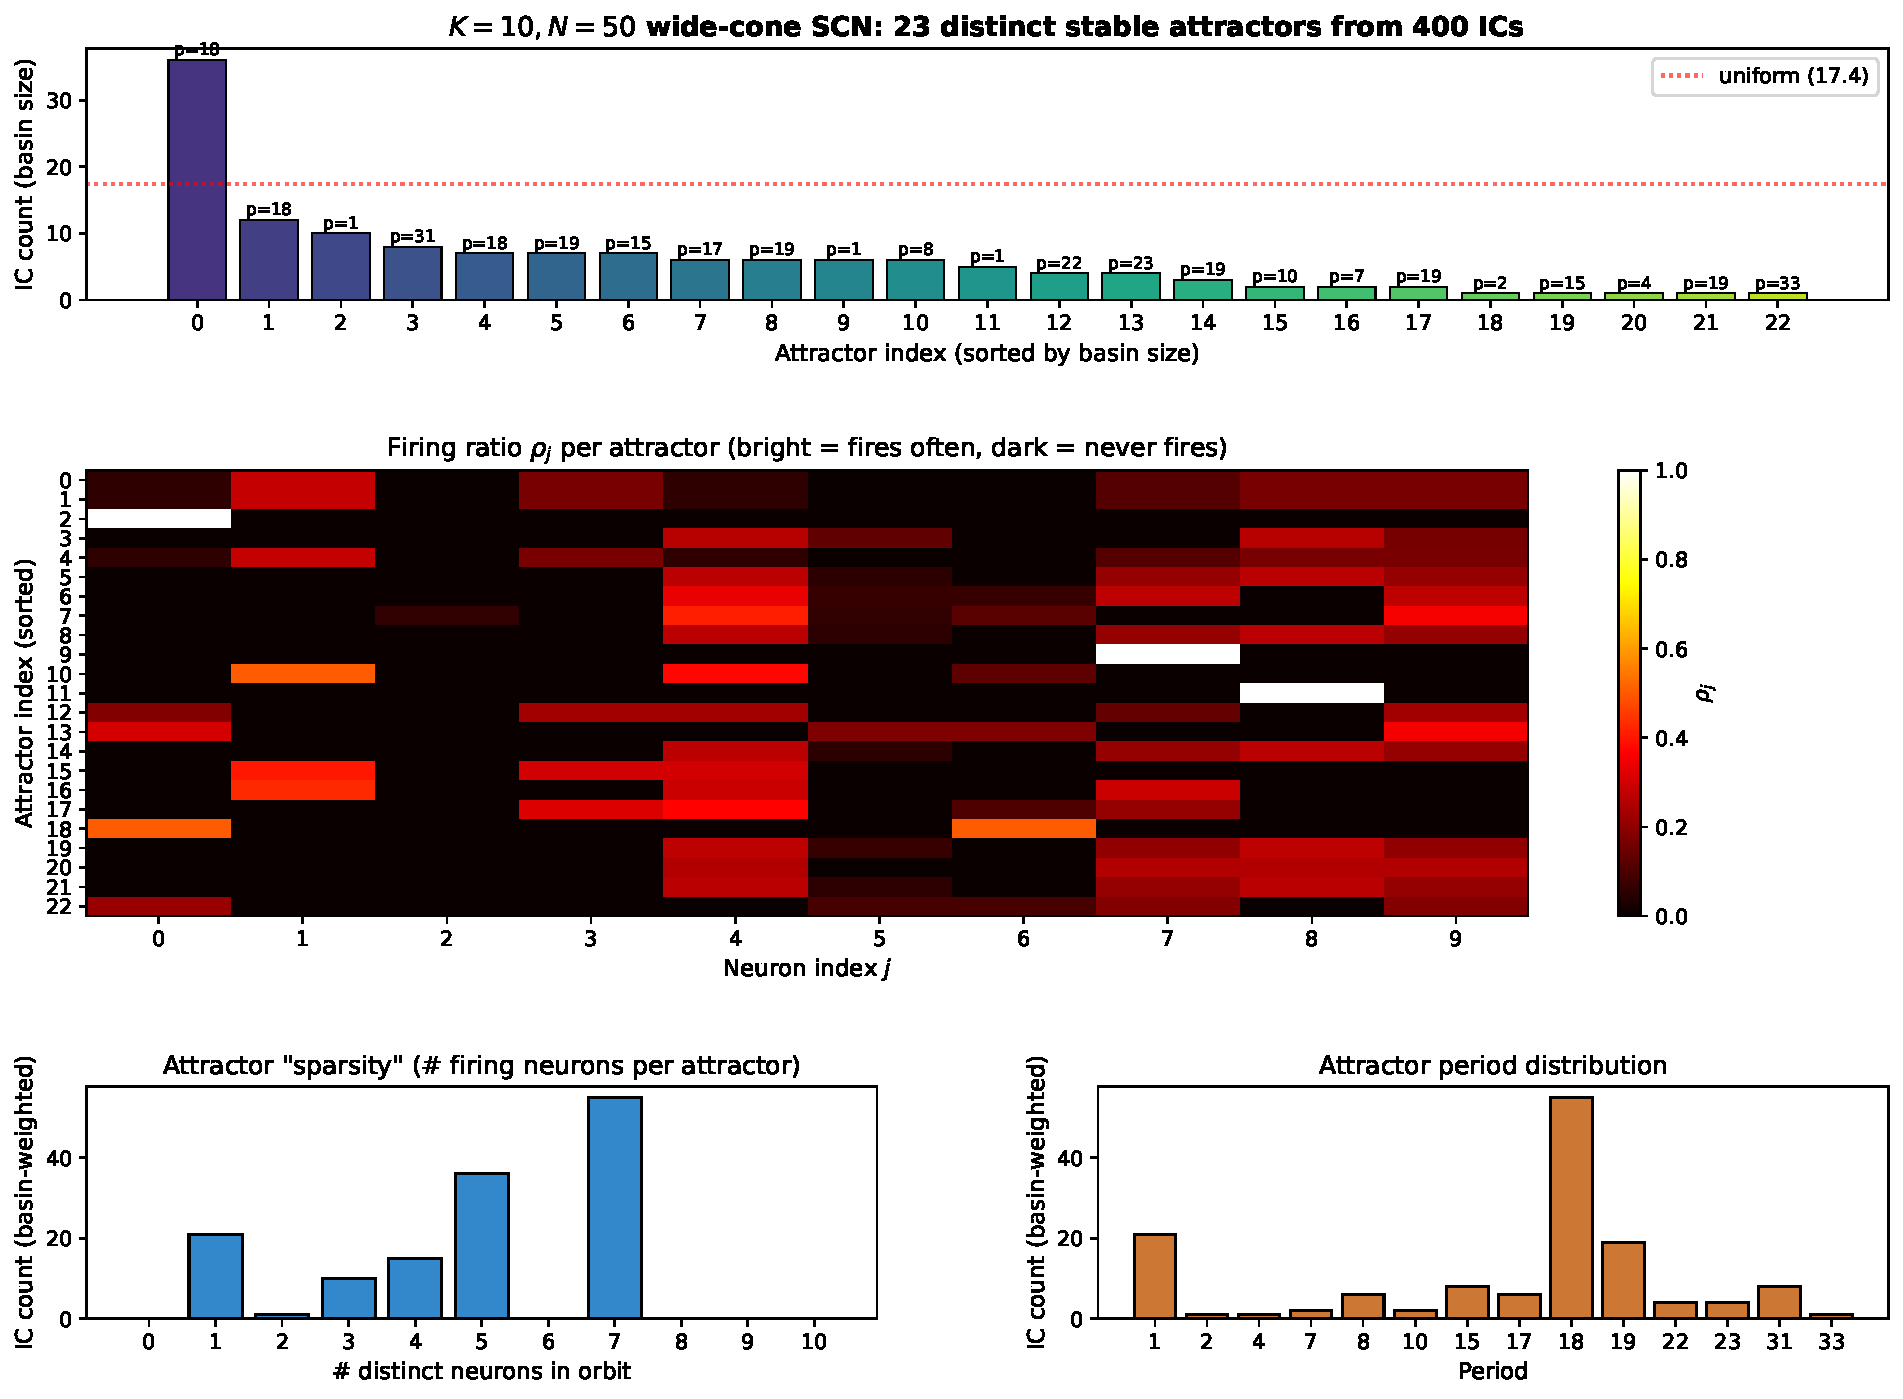
\includegraphics[width=\textwidth]{figures/multistability_highD}
\caption{Wide-cone $K=10$, $N=50$ SCN: basin survey over 400 random initial conditions reveals 23 distinct stable attractors. \textbf{Top:} basin size per attractor (sorted). \textbf{Middle:} firing-ratio $\rho_j$ per attractor (heatmap: attractor $\times$ neuron). Rows with identical rows share the same DC readout $\bar{\vv{y}}$ (spike-timing degeneracy compatible with Mancoo's readout uniqueness); distinct rows reveal genuine multistability at the readout level. \textbf{Bottom-left:} number of firing neurons per attractor. \textbf{Bottom-right:} attractor-period distribution. Complements Table~\ref{tab:wide-cone-atlas}, which lists the top~$8$ basins.}
\label{fig:multi-highD}
\end{figure}

\begin{figure}[ht]
\centering
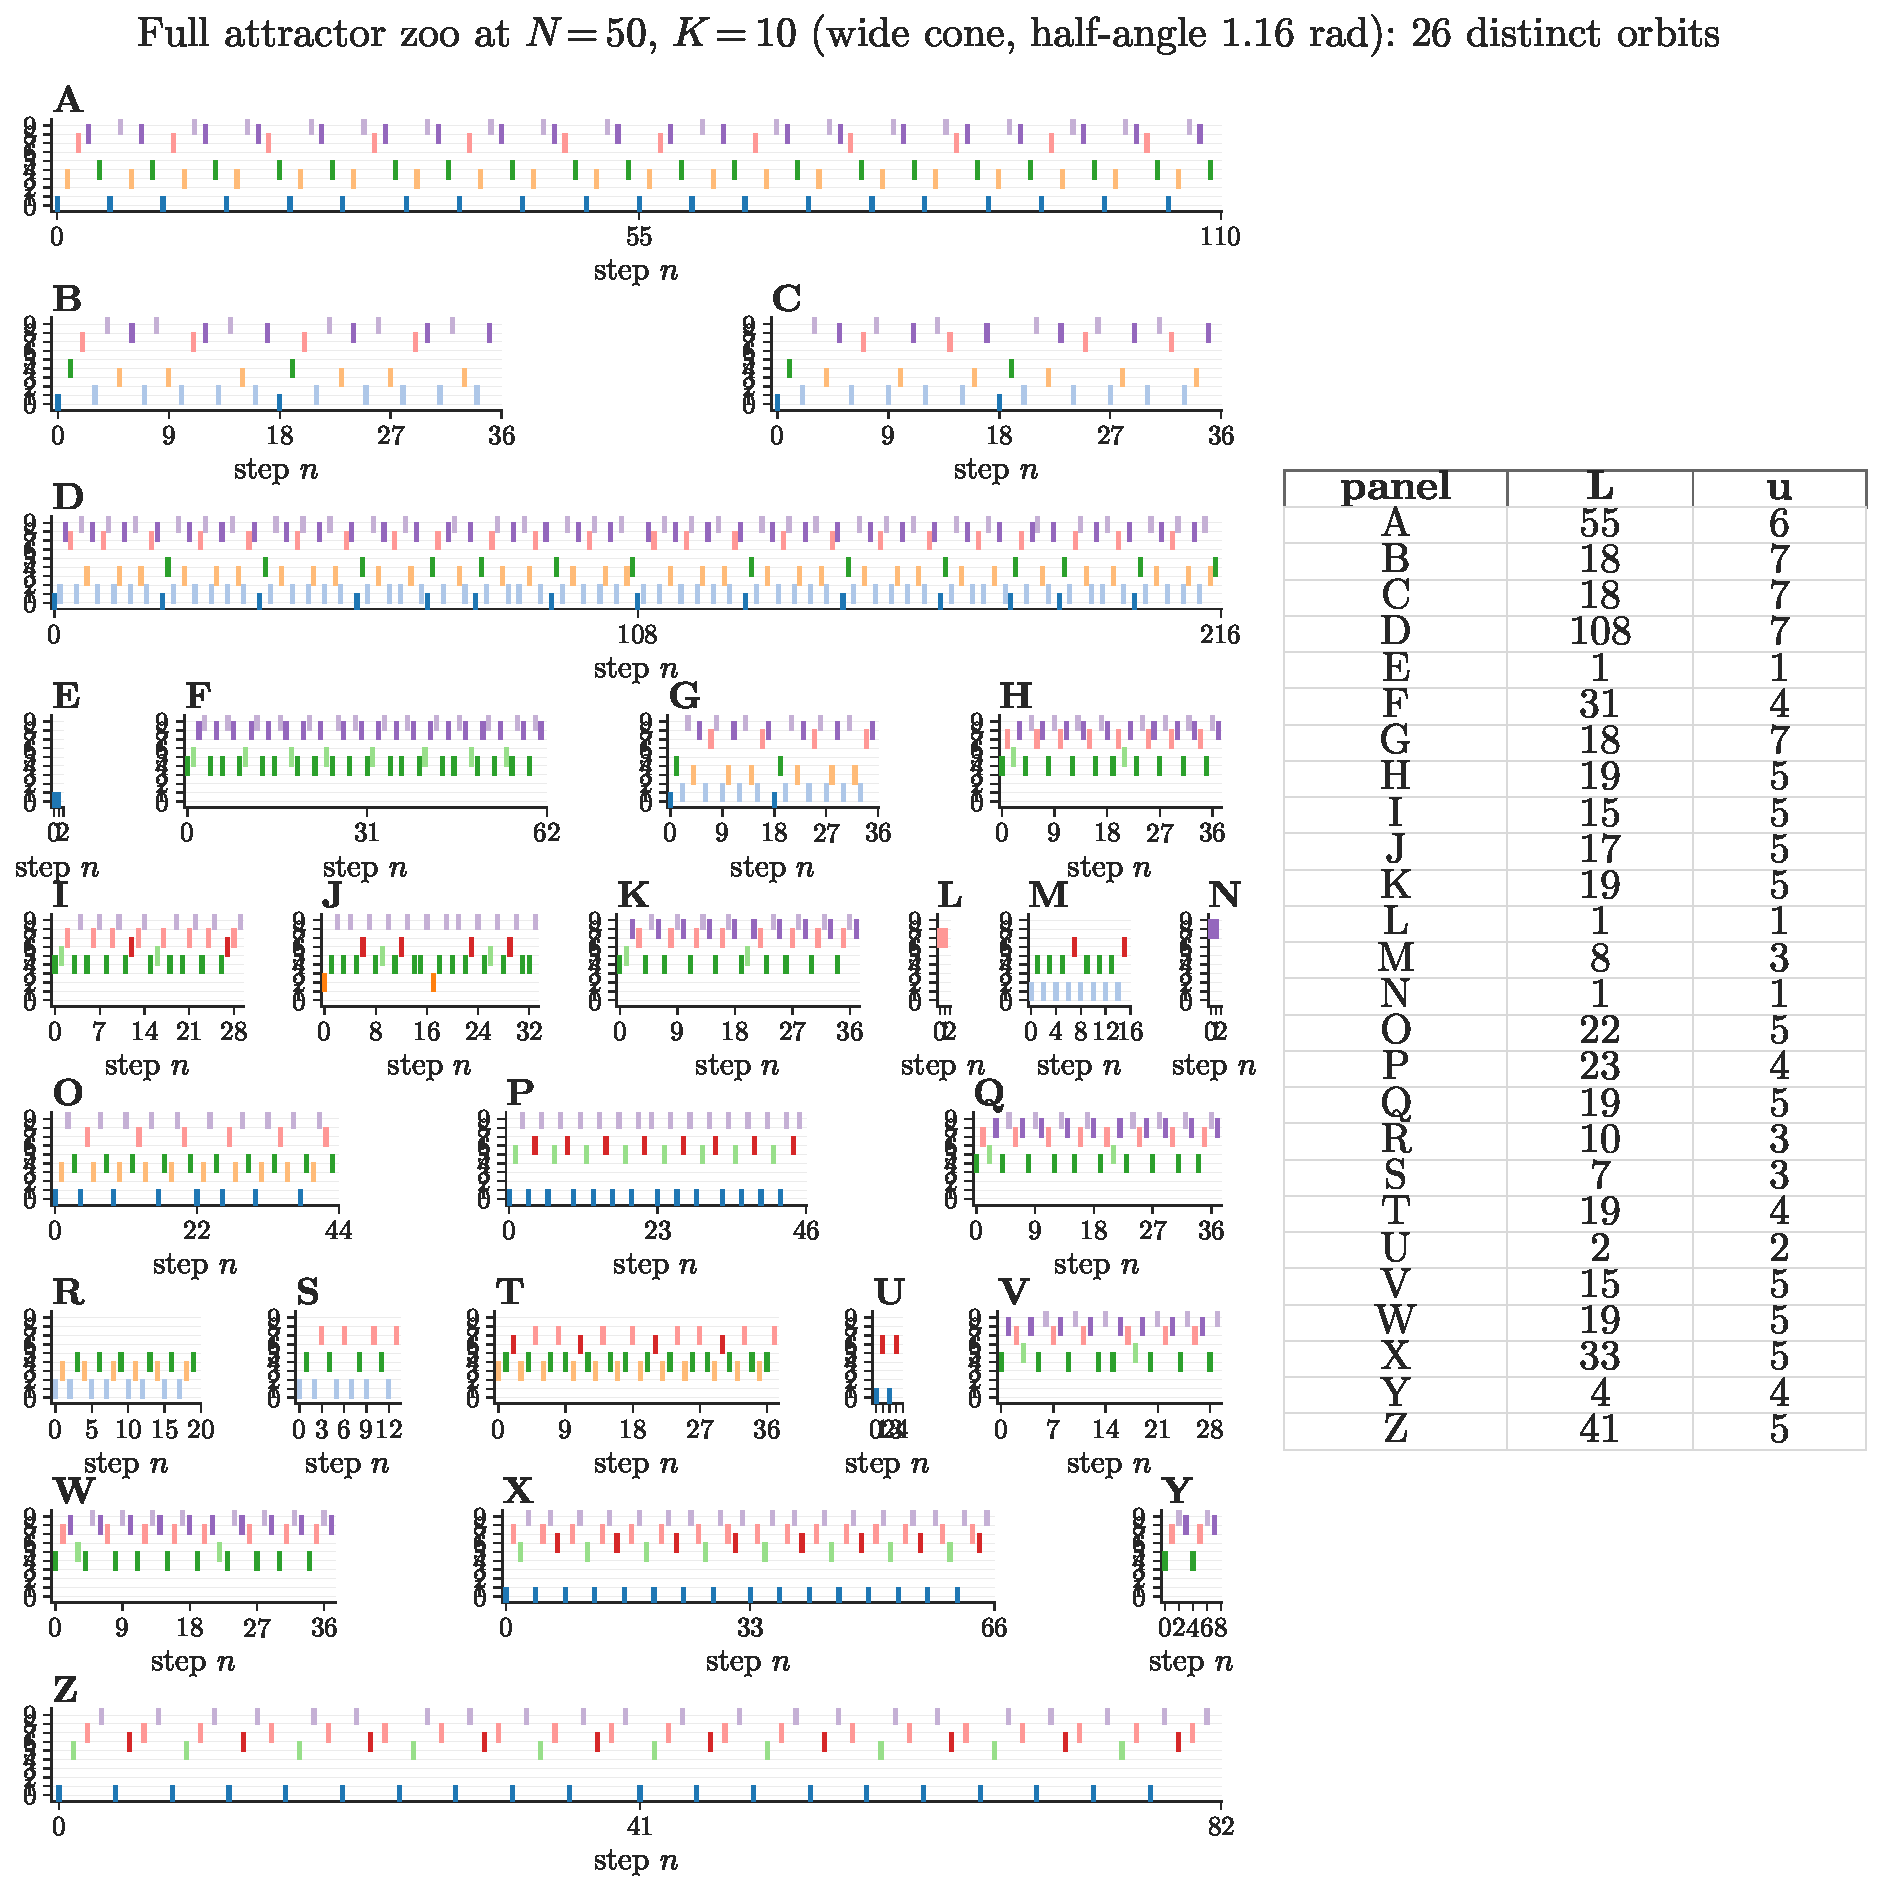
\includegraphics[width=\textwidth]{figures/orbit_zoo_wide_N50.pdf}
\caption{Full attractor zoo at $N{=}50$, $K{=}10$, half-angle $1.16$~rad: spike raster of every distinct stable periodic orbit found, with panel widths scaled to period. The $[\mathrm{S}]$ tag (``short'') marks orbits with period $p\leq 40$ discovered by the $400$-IC short-burn-in survey ($6\,000$ burn-in steps); the $[\mathrm{L}]$ tag (``long'') marks orbits with period $p\geq 33$ discovered only by the extended-burn-in pass ($20\,000$ burn-in steps) on basin-map cells that the short pass left unclassified.}
\label{fig:orbit-zoo-wide}
\end{figure}

\begin{figure}[ht]
\centering
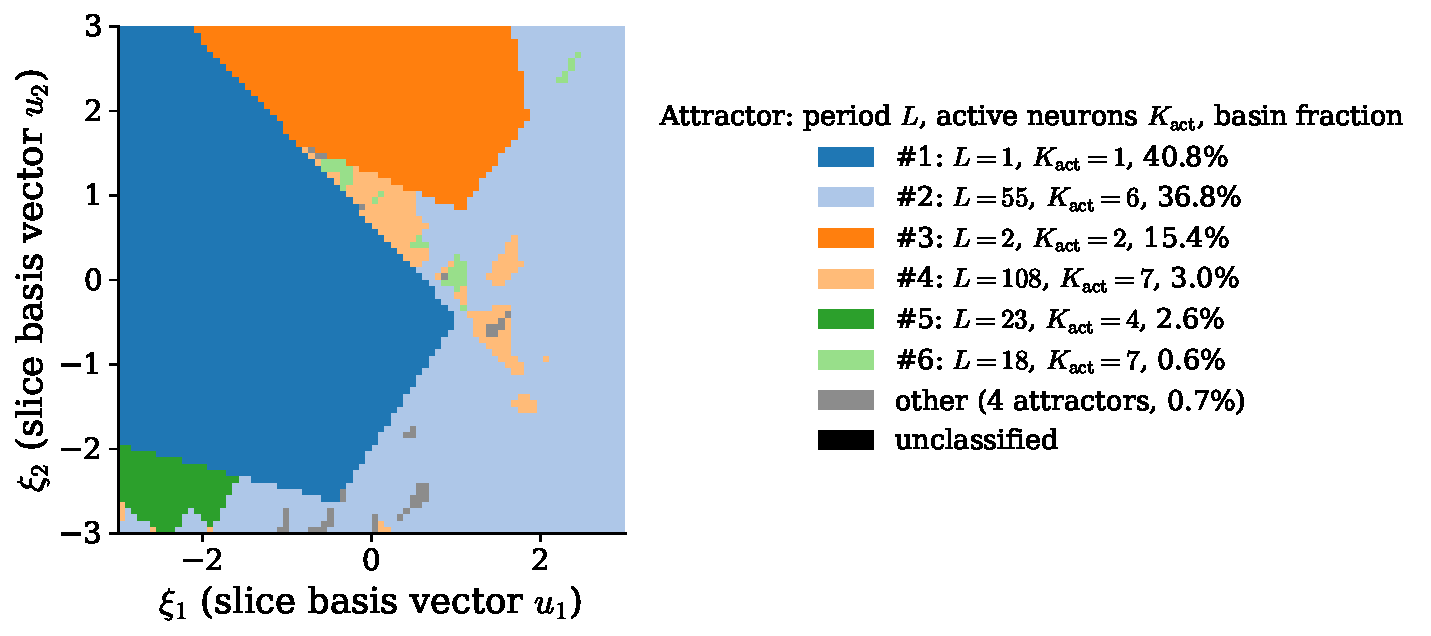
\includegraphics[width=0.75\textwidth]{figures/basin_map_wide.pdf}
\caption{Basin map of the wide-cone $N{=}50$, $K{=}10$ SCN (cone half-angle $1.16$~rad) on a random $2$D slice of the $49$-dimensional tangent space on $\mathcal{B}_1$: axes $\xi_1,\xi_2$ are coordinates in an orthonormal slice basis $(u_1,u_2)$; a point $(\xi_1,\xi_2)$ corresponds to the tangent state $\xi_1 u_1+\xi_2 u_2$. Each grid cell is coloured by the periodic attractor its orbit converges to (short- and long-period orbits merged); $10$ distinct attractors are resident on the slice. The $6$ largest basins are shown individually; the remaining $4$ are grouped as ``other''. Legend: $L$ is the period (letters per cycle) and $K_{\mathrm{act}}$ the number of distinct neurons that fire in the cycle. Every grid cell is classified — no diverging trajectories.}
\label{fig:basin-map-wide}
\end{figure}

\subsection{Self-transition runs}\label{app:self-trans}

A run of $k$ consecutive self-firings by neuron~$i$ contracts the tangent coordinate as $\xxi\mapsto(\alpha_i/(\alpha_i+1))^k\xxi$, pulling the orbit toward the foot $\xxi=\vv{0}$. Since the self-decay factor $c_i=\alpha_i/(\alpha_i+1)$ is constant (independent of $\xxi$), while the cross-transition factor $c_j=\alpha_j/(\DD_j^\top\yy^+)$ depends on $\xxi$ through the denominator, each self-firing shifts the relative ordering of the decay factors. The orbit self-fires until the contraction pushes $\xxi$ across a partition boundary (where $c_i=c_j$ for some $j\neq i$), at which point a cross-transition occurs. The run length is approximately $k \approx (\ln|\xxi_{\text{arrive}}| - \ln|\xxi_{\text{part}}|)/\ln((\alpha_i+1)/\alpha_i)$. Since self-transitions only contribute contractive factors $(\alpha_i/(\alpha_i+1))^k<1$ to the return map, words with longer self-transition runs are generically more stable.

\section{Analytical proofs and corollaries}\label{app:proofs}

\subsection{Birkhoff's ergodic theorem}\label{app:birkhoff}

We invoke the following classical result at several points in the main text (Section~\ref{sec:sturmian-chain}, Theorem~\ref{thm:cone}).

\begin{theorem}[Birkhoff's ergodic theorem]\label{thm:birkhoff}
Let $(X,\mathcal{F},\mu)$ be a probability space and let $T:X\to X$ be a measurable transformation that preserves $\mu$, i.e.\ $\mu(T^{-1}A)=\mu(A)$ for every $A\in\mathcal{F}$. For every $f\in L^1(\mu)$, the limit
\begin{equation}\label{eq:birkhoff}
\bar f(x)\;=\;\lim_{n\to\infty}\frac{1}{n}\sum_{k=0}^{n-1}f(T^kx)
\end{equation}
exists for $\mu$-almost every $x\in X$; the limit function $\bar f$ is $T$-invariant ($\bar f\circ T=\bar f$ $\mu$-a.e.); and $\int_X\bar f\,d\mu=\int_X f\,d\mu$. If in addition $T$ is \emph{ergodic} (every $T$-invariant set has measure 0 or 1), then $\bar f$ is constant $\mu$-a.e.\ and equals $\int_X f\,d\mu$; in particular, for any measurable set $A\in\mathcal{F}$,
\[
\lim_{n\to\infty}\frac{1}{n}\sum_{k=0}^{n-1}\mathbf{1}_A(T^kx)\;=\;\mu(A)\quad\text{for $\mu$-a.e.\ }x.
\]
\end{theorem}

The original references are \citet{birkhoff1931proof} and \citet{vonneumann1932proof} (mean ergodic theorem); modern textbook treatments include \citet{walters2000introduction} and \citet{petersen1983ergodic}. In our setting, $X=\Bsp_1\cup\{\infty\}$, $T=F_{\!\Bsp_1;\alpha_2}$ is the first-return piecewise-M\"obius map (Proposition~\ref{prop:circle-homeo}), $\mu=\mu_F$ is its unique invariant probability measure on the class-$\mathcal L$ side (which exists and is unique for orientation-preserving circle homeomorphisms with irrational rotation number; \citealp{herman1979conjugaison}), and the observable $f=\mathbf{1}_{P_2}$ is the indicator of the cross-transition cell. Applying~\eqref{eq:birkhoff} identifies the long-run firing ratio $\rho$ with the invariant mass $\mu_F(P_2)$, which is the identity used to align the SCN's partition with the rotation number in Section~\ref{sec:sturmian-chain}, Step~3.

\subsection{Vanishing Lyapunov exponent at irrational rotation number}\label{app:quasi-LE}

\begin{proposition}[Vanishing Lyapunov exponent at irrational rotation number, $K{=}2$]\label{prop:quasi-LE}
For the $K{=}N{=}2$ SCN in the cone-preserving regime ($\cos\psi>0$), let $F_{\alpha_2}$ be the first-return piecewise-M\"obius map (Proposition~\ref{prop:circle-homeo}) at drive $\alpha_2$ in the admissibility window, and suppose $\rho:=\rho(\alpha_2)$ is irrational. Call $\rho$ \emph{Diophantine of exponent~$\tau\geq 0$} if there exists $C>0$ such that $|\rho-p/q|\geq C\,q^{-2-\tau}$ for every rational $p/q$. Assume either of the following:
\begin{enumerate}[label=(\alph*),nosep]
    \item \emph{(Smooth case, Herman--Yoccoz)} $\rho$ is Diophantine and $F_{\alpha_2}$ is $C^2$ off its break point \citep{herman1979conjugaison,yoccoz1984conjugaison}.
    \item \emph{(Piecewise-M\"obius case, Liousse)} $\rho$ is Diophantine and the Boshernitzan invariant of the break-point derivative jump, $\log\bigl(F'(\xi_{\mathrm{part}}^+)/F'(\xi_{\mathrm{part}}^-)\bigr)$, satisfies the trivial-holonomy condition of \citet{liousse2005nombre} (which reduces to $F'(\xi_{\mathrm{part}}^+)=F'(\xi_{\mathrm{part}}^-)$ in the constant-slope case).
\end{enumerate}
Under either hypothesis the unique $F_{\alpha_2}$-invariant probability measure $\mu_F$ is absolutely continuous with respect to Lebesgue, and the Lyapunov exponent of the discrete return map satisfies
\begin{equation}\label{eq:LE-quasiperiodic}
\lambda(F_{\alpha_2},\mu_F) \;=\; \int_{\Bsp_1} \log|F'_{\alpha_2}(x)|\,d\mu_F(x) \;=\; 0.
\end{equation}
\end{proposition}

\begin{proof}
Let $f>0$ be the density of $\mu_F$ with respect to Lebesgue (existing under the AC hypothesis). $F_{\alpha_2}$-invariance, $\mu_F(F^{-1}(A))=\mu_F(A)$, gives the density-change equation
\[
f(F(x))\,|F'(x)| \;=\; f(x)
\]
for $\mu_F$-a.e.\ $x$. Taking logarithms,
\[
\log|F'(x)| \;=\; \log f(x) - \log f(F(x)),
\]
and integrating against $\mu_F$,
\[
\int\log|F'|\,d\mu_F \;=\; \int\log f\,d\mu_F - \int(\log f\circ F)\,d\mu_F \;=\; 0,
\]
where the last equality uses $F$-invariance of $\mu_F$ in the second integral.
\end{proof}

\paragraph{Discrete return-map LE vs.\ continuous-time flow LE.}
Equation~\eqref{eq:LE-quasiperiodic} gives the Lyapunov exponent of the \emph{discrete} return map $F$. The full continuous-time SCN flow on $\bigsqcup_i\Bsp_i$ has its own Lyapunov spectrum: it acquires one additional zero exponent in the time-translation direction (a generic property of any smooth limit-cycle-like dynamics, exploited as a working-memory substrate in \citealp{Park2023a}), while the discrete return map's transverse exponents $\log|\mu_k/\mu_1|<0$ become the flow's transverse exponents scaled by the average period. Both pictures give the same headline conclusion, $\lambda_{\max}=0$ at a quasi-periodic orbit, but via different mechanisms: measure preservation of the return map for the discrete picture, time-translation symmetry along the cycle for the flow picture.

\paragraph{Restriction to $K{=}2$.} Proposition~\ref{prop:quasi-LE} is stated only for $K{=}2$. For $K\geq 3$, the first-return map acts on a $(N{-}1)$-dimensional bound rather than a 1D circle; there is no single rotation number but a rotation \emph{vector} on a higher-dimensional torus, and the Herman--Liousse conjugacy theory generalises into the more delicate Yoccoz--Khanin framework for circle-of-tori maps. The corresponding zero-Lyapunov-exponent statement is not addressed here.

\subsection{Dale's-law geometry (proof sketch, kept for reference)}\label{app:dale-proof}

For a hypothetical Dale-compatible SCN under the connectivity $W_{ij}=-\DD_i^\top\DD_j$ (the main-text Dale-law paragraph is commented out; this proof sketch is retained for reference). If neuron $j$ is inhibitory, $W_{ij}=-\DD_i^\top\DD_j\leq 0$ for all~$i$, hence $\DD_i^\top\DD_j\geq 0$ for all~$i$. If neuron $k$ is excitatory, $W_{ik}=-\DD_i^\top\DD_k\geq 0$ for all~$i$, hence $\DD_i^\top\DD_k\leq 0$ for all~$i$. Taking $i=j$ (inhibitory): $\DD_j^\top\DD_k\leq 0$; taking $i=k$ (excitatory): $\DD_k^\top\DD_j\geq 0$. Both require $\DD_j^\top\DD_k=0$. Sign constraints within each population plus the classical result that at most $N+1$ unit vectors in $\RR^N$ can have all-negative pairwise inner products give the simplex bound $K_E\leq N+1$.

\subsection{Farey cascade to the singular parameter $\alpha_1^*$ for $\rho=1/\pi$}\label{app:pi-cascade}

For $K{=}N{=}2$ at $\psi=0.4\pi$, $\alpha_0=1$, the rotation number $\rho(\alpha_1)$ traces a complete devil's staircase (Section~\ref{sec:bifurcation}).
Irrational $\rho$ are achieved on a measure-zero set; we locate the singular $\alpha_1^*$ realizing $\rho=1/\pi$ by walking a Farey cascade of rational plateaus toward it.
The continued-fraction expansion of $1/\pi$ is $[0;3,7,15,1,292,\ldots]$, so the convergents are $1/3,7/22,106/333,113/355$, with semi-convergents $(7m{+}1)/(22m{+}3)$ filling the path from $7/22$ to $106/333$ as $m=1,\ldots,15$.

\paragraph{Method.}
For any rational $\rho=p/q$ with $\gcd(p,q)=1$, the unique balanced firing word is the mechanical Sturmian
$\sigma_{p/q}=(s_0,\ldots,s_{q-1})$ with $s_k=\lfloor(k{+}1)p/q\rfloor-\lfloor kp/q\rfloor\in\{0,1\}$.
Building the $2\times 2$ symbolic return matrix
$\vv{M}_\sigma(\alpha_1)=\prod_{k=q-1}^{0}\vv{M}_{s_{k+1}\leftarrow s_k}(\alpha_1)$ in $300$-digit \texttt{mpmath} and dehomogenizing its dominant eigenvector gives the predicted orbit $(\xi_0,\ldots,\xi_{q-1})$.
The orbit is realized iff the admissibility margin
\begin{equation}\label{eq:cascade-margin}
m(\alpha_1)\;=\;\min_{k}\Bigl(c_{s_{k+1}}-\!\!\max_{j\ne s_{k+1}}c_j\Bigr)
\end{equation}
is positive at the predicted orbit, where the decay factors $c_j=\alpha_j/(\DD_j^\top\yy_k^+)$ are evaluated at each post-spike readout~$\yy_k^+$. The plateau is then $\{\alpha_1:m(\alpha_1)>0\}$.

We bisect both edges of each plateau in turn, walking down the Farey chain:
the left bracket at level $(p_n,q_n)$ is the precisely refined right edge of $7/22$,
\[\alpha_1^{(7/22)\mathrm{R}}=0.5223343802940303852301165223341492397534560143394308644640508665058751\ldots\] (computed first at \texttt{mpmath} $\textsf{dps}=300$), and the right bracket is the previous level's left edge.

\begin{figure}[h]
\centering
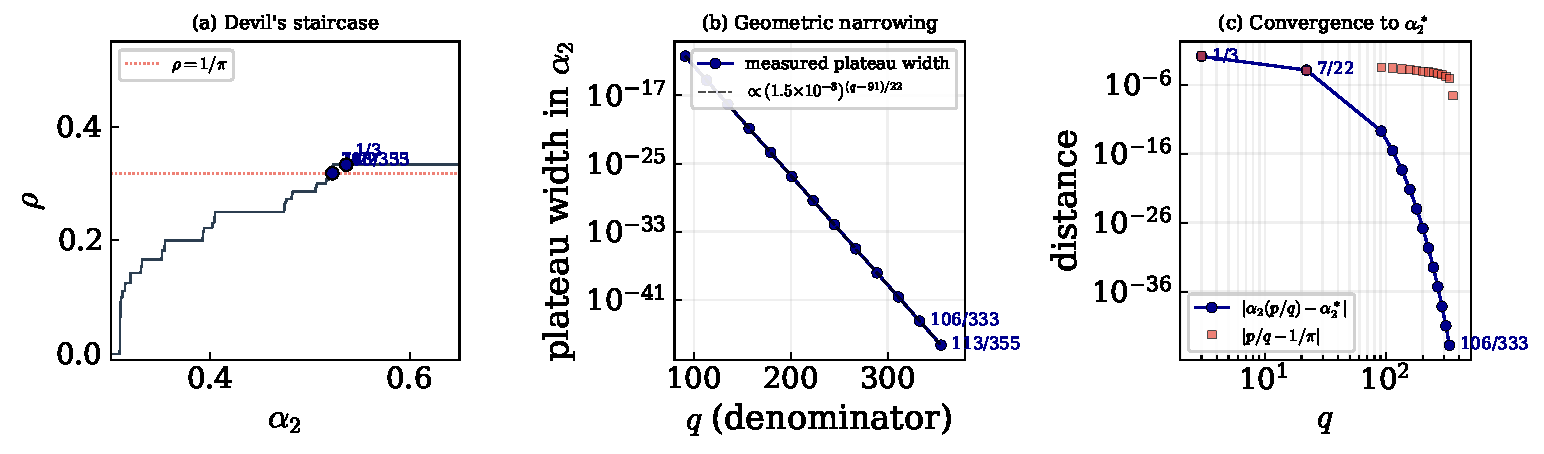
\includegraphics[width=0.95\textwidth]{figures/pi_approximants.pdf}
\caption{Farey cascade toward $\rho=1/\pi$. \textbf{(a)}~The devil's staircase with the four continued-fraction convergents marked. \textbf{(b)}~Plateau widths in $\alpha_1$ along the Farey chain decay geometrically by ${\sim}1.5\times 10^{-3}$ per step of $q$ by $22$. \textbf{(c)}~The plateau centres' distance to the cascade limit $\alpha_1^*$, alongside $|p/q-1/\pi|$ for comparison; both follow the same super-polynomial convergence.}
\label{fig:pi_approximants}
\end{figure}

\paragraph{Results.}
The 13~plateaus from $29/91$ down to the convergent $113/355$ all admit positive-width plateaus of unambiguously detectable width (Table~\ref{tab:cascade}, Figure~\ref{fig:pi_approximants}). Plateau widths decay geometrically by a factor of $\approx 1.5\times 10^{-3}$ per Farey step (each step adds $22$ to $q$), so the convergent $113/355$ has plateau width $4.95\times 10^{-47}$ in $\alpha_1$, far below the $10^{-16}$ double-precision floor that defeats simulation-based searches.

\begin{table}[h]
\centering
\begin{tabular}{rcc}
\hline
$\rho=p/q$ & $q$ & plateau width \\
\hline
$29/91$    &  91 & $3.99\times 10^{-13}$ \\
$36/113$   & 113 & $5.96\times 10^{-16}$ \\
$43/135$   & 135 & $8.91\times 10^{-19}$ \\
$50/157$   & 157 & $1.33\times 10^{-21}$ \\
$57/179$   & 179 & $1.99\times 10^{-24}$ \\
$64/201$   & 201 & $2.97\times 10^{-27}$ \\
$71/223$   & 223 & $4.45\times 10^{-30}$ \\
$78/245$   & 245 & $6.64\times 10^{-33}$ \\
$85/267$   & 267 & $9.93\times 10^{-36}$ \\
$92/289$   & 289 & $1.48\times 10^{-38}$ \\
$99/311$   & 311 & $2.22\times 10^{-41}$ \\
$106/333$  & 333 & $3.32\times 10^{-44}$ \\
$113/355$  & 355 & $4.95\times 10^{-47}$ \\
\hline
\end{tabular}
\caption{Plateau widths along the Farey cascade toward $\rho=1/\pi$, computed in \texttt{mpmath} at $300$-digit precision. Each step from $q$ to $q{+}22$ shrinks the plateau by ${\sim}1.5\times 10^{-3}$.}
\label{tab:cascade}
\end{table}

\paragraph{The singular point.}
Along the cascade, the right edge of $113/355$ and the left edge of $106/333$ coincide to all $\sim 80$~digits resolved in our run, giving the cascade limit
\begin{equation}
\alpha_1^*\;\approx\;0.522334380294030385230116522334149239753456014389052084833331820664863883\ldots
\end{equation}
This is the unique $\alpha_1$ at which the SCN has rotation number exactly $1/\pi$: the firing word is the aperiodic Sturmian $\sigma_{1/\pi}$ and the orbit closure has empty interior on $\Bsp_0$.

\paragraph{Irrational firing ratios are realized; finite-precision simulation only sees rational ones.}
The rotation number $\rho(\alpha_1)$ is continuous and monotone non-decreasing in $\alpha_1$ on this family (Section~\ref{sec:bifurcation}; \citealp{herman1979conjugaison}). It takes the value $0$ at small $\alpha_1$ and rises through $1/2$ at large $\alpha_1$. By the intermediate value theorem, $\rho$ attains \emph{every} real value in $[0,1/2]$ --- every rational, every algebraic and transcendental irrational --- so for each target $\omega\in[0,1/2]$ there exists $\alpha_1^*(\omega)$ realizing it.\footnote{Uniqueness up to plateau interior: for rational $\omega=p/q$, all $\alpha_1$ in the plateau realize $\omega$; for irrational $\omega$ the realization is at a single point.} Rational $\omega$ are realized on plateaus of positive Lebesgue measure; irrational $\omega$ are realized at single points forming a Cantor-like measure-zero set. The dynamics at every $\alpha_1$ is well defined --- deterministic update law, real-valued state, Birkhoff average converging to $\rho(\alpha_1)$ --- including at every irrational realization. What finite-precision simulation cannot do is \emph{set} $\alpha_1$ to a singular value: a double-precision $\alpha_1$ lies within $10^{-16}$ of its representable neighbour, and the plateaus have full Lebesgue measure in any region of the staircase, so round-off lands on a rational. Reaching $\alpha_1^*(1/\pi)$ requires the Farey cascade --- approaching the singular parameter from a sequence of computable rational neighbours at extended precision.

\paragraph{The cascade is the theory.}
$\alpha_1^*$ has no known closed-form expression --- the cascade itself is the canonical characterization. Three equivalent definitions all reduce to the same infinite procedure.

\emph{(i) As an inverse rotation number.} $\alpha_1^*$ is uniquely defined by $\rho(\alpha_1^*) = 1/\pi$, where the rotation number is the Birkhoff limit
\[
\rho(\alpha_1) \;=\; \lim_{n\to\infty} \frac{1}{n}\sum_{k=0}^{n-1} \mathbf{1}_{\{\text{neuron 1 fires at step } k\}}.
\]
Inverting a Birkhoff limit is itself an infinite procedure: $\alpha_1^*$ is a limit of limits.

\emph{(ii) As a topological conjugacy.} The natural rigidity statement is \textbf{Denjoy's theorem} \citep{denjoy1932courbes}: \emph{every orientation-preserving $C^2$ diffeomorphism $F$ of the circle with irrational rotation number $\rho$ is topologically conjugate to the rigid rotation $R_\rho(x)=x+\rho\pmod 1$ --- that is, there exists an orientation-preserving homeomorphism $h$ of the circle with $h\circ F\circ h^{-1}=R_\rho$} (see also \citealp{herman1979conjugaison}). The conjugacy is at most $C^0$, not analytic. Applied at $\alpha_1^*$ (rotation number $1/\pi$) it would give $F_{\alpha_1^*}$ conjugate to $R_{1/\pi}$. Two caveats. First, the SCN return map is continuous and piecewise M\"obius but only $C^0$ at the partition point $\xi_{\mathrm{part}}$, so the $C^2$ hypothesis of the classical theorem fails. Piecewise-smooth extensions \citep{liousse2005nombre} restore the conclusion provided no break point lies on the orbit closure; we do not verify this condition for the SCN, and record it as the natural sufficient hypothesis under which $\alpha_1^*$ corresponds to dynamics genuinely conjugate to rotation rather than to a Denjoy counter-example with a Cantor-set attractor. Second, in either case the conjugacy $h$ is at most $C^0$ and has no known closed-form expression, so it provides no analytic shortcut to $\alpha_1^*$.

\emph{(iii) As a constant defined by an infinite cascade.} A clean analogue is the \textbf{Feigenbaum bifurcation constant} of period-doubling: for a one-parameter family $f_r$ with a quadratic maximum (e.g.~the logistic map $f_r(x)=rx(1-x)$), let $r_1<r_2<\cdots$ be the parameter values at successive period-doubling bifurcations on the route to chaos. The ratio
\[
\delta \;=\; \lim_{n\to\infty}\frac{r_n-r_{n-1}}{r_{n+1}-r_n} \;\approx\; 4.66920160910299\ldots
\]
is a specific real number defined entirely by this limit and is universal across families with quadratic maxima \citep{feigenbaum1978quantitative}. No closed form is known for $\delta$; it is computable to arbitrary precision only by walking the cascade. Our $\alpha_1^*(1/\pi)$ is of the same character: a specific real number defined by an infinite Farey cascade, with no known closed form, computable only by walking the cascade to the required depth. Each Farey level here adds ${\sim}\log_{10}(1.5{\times}10^{-3})^{-1}\approx 2.8$ digits of $\alpha_1^*$; stopping at $113/355$ gives the ${\sim}50$ verified digits reported above. The next CF convergent $33102/103993$ has plateau width $\sim 10^{-1\,400}$, beyond any feasible computation.


\subsection{Chaos mechanism: stable but inadmissible periodic orbits}\label{app:chaos-mechanism}

In the chaotic regime ($\cos\psi_{\min}=-0.57$), every short periodic sub-word observed in the chaotic trajectory has a return map $\vv{M}_\sigma$ whose dominant eigenvector is mathematically \emph{stable} ($|\mu_2/\mu_1|<1$). For example, the word $(2,3)$ has $|\mu_2/\mu_1|=0.62$, word $(1,2)$ has $0.22$, word $(0,2)$ has $0.41$. Yet none of these fixed points are admissible: at some step in the candidate orbit, a different neuron would fire first. This pattern holds for all 30 most-visited sub-words of lengths 2--7.

The chaos therefore arises not because individual periodic orbits are unstable (they are all stable), but because the partition prevents the trajectory from settling into any of them. Each candidate orbit's fixed point lies outside the admissible region for its word, so the trajectory is perpetually deflected at partition boundaries. The piecewise switching between branches produces a net positive expansion ($\lambda_1=0.285$) even though each branch's own dynamics would be contracting.

This mechanism differs from smooth chaos (e.g.\ Smale horseshoes), where the attractor is woven from unstable periodic orbits. Here the periodic orbits exist with stable eigenvalues but are blocked by the combinatorial constraint of admissibility. The local Lyapunov (expanding) direction rotates across the attractor (standard deviation $88^\circ$, range $243^\circ$), confirming that no fixed direction is responsible for the expansion. Chaotic dynamics in neural circuits have been proposed as a substrate for probabilistic computation through sampling \citep{terada2024chaotic} and have been experimentally observed in cortical recordings \citep{korn2003there,sarbadhikari2001chaos}.

\paragraph{The algebraic machinery is regime-agnostic; only its meaning changes.}
The $\sigma\mapsto\vv{M}_\sigma\mapsto(\text{eigenvalues},\text{eigenvector}\mapsto\xi^*)$ construction is a polynomial-coefficient algebraic procedure that requires no positivity hypothesis and is therefore the same in both regimes. What changes are which guarantees still hold and what the predicted $\xi^*$ \emph{means} dynamically. Table~\ref{tab:cone-vs-chaos} summarizes.

\begin{table}[h]
\centering
\renewcommand{\arraystretch}{1.2}
\begin{tabular}{p{0.32\linewidth}p{0.28\linewidth}p{0.30\linewidth}}
\hline
\textbf{Property} & \textbf{Cone-preserving regime} ($\cos\psi_{ij}>0$ all $i,j$) & \textbf{Chaos regime} ($\cos\psi_{ij}<0$ some $i,j$) \\
\hline
$\vv{M}_\sigma$ construction & polynomial in parameters: same formula & polynomial in parameters: same formula \\
Dominant eigenvalue $\mu_1$ & simple, real, positive (Perron--Frobenius) & not guaranteed; can be complex pair, negative, or non-simple \\
Eigenvector in positive cone $\mathcal{C}$ & yes & not guaranteed \\
Hilbert-metric contraction $|\mu_k/\mu_1|<1$ & yes, uniform over orbit & breaks in general; can persist algebraically (as in our $K{=}4$ example) without giving an attractor \\
Admissibility of the $\sigma$-orbit at the predicted $\xi^*$ & one $\sigma$ admissible per parameter (locked on each plateau, Cor.~\ref{cor:within-plateau}) & generically fails for any short $\sigma$ observed in the trajectory: the predicted $\xi^*$ lies outside the partition cell of its own next firer \\
What the predicted $\xi^*$ is dynamically & the system's unique attracting periodic orbit & a (typically algebraically stable but \emph{inadmissible}) candidate that the trajectory perpetually deflects away from at partition boundaries \\
Source of complexity & smooth M\"obius branches; Arnold-tongue widths & partition-induced switching between branches; no fixed expanding direction \\
Number of admissible $\sigma$ at period $L$ & exactly one (the Sturmian $\sigma_{p/q}$ of the plateau) & system-dependent; in our example, no short admissible $\sigma$ is realized as a stable cycle \\
\hline
\end{tabular}
\caption{The eigenvector-orbit construction $\sigma\mapsto\xi^*$ runs identically in both regimes; what differs is which classical guarantees survive and what dynamical role the predicted $\xi^*$ plays.}
\label{tab:cone-vs-chaos}
\end{table}

\subsection{Robustness bound via eigenvector perturbation theory}\label{app:robustness}

For the RBYGYB orbit, the $3\times 3$ return map $\vv{M}_\sigma$ has right eigenvectors $\vv{u}_k$ and left eigenvectors $\vv{w}_k$ (normalized so $\vv{w}_k^\top\vv{u}_k=1$). Under a drive perturbation $\delta\alpha_j$, the return map shifts by $\delta\vv{M}=(\partial\vv{M}_\sigma/\partial\alpha_j)\delta\alpha_j$. The first-order eigenvector perturbation~\eqref{eq:eigpert} predicts the orbit shift $\delta\xxi^*$.

\textbf{Validation:} The predicted $\|\delta\xxi^*/\delta\alpha_j\|$ matches the numerically computed sensitivity to 4 significant figures for all four drives ($\text{ratio}\approx 1.000$), confirming the first-order theory is essentially exact.

\textbf{Tolerance bound:} The orbit survives perturbation $\delta\alpha_j$ iff the margin remains positive. The per-drive tolerance is $|\delta\alpha_j|_{\max}\approx m/|\partial m/\partial\alpha_j|$, where the margin gradient is computed by finite differences. Results:

\begin{center}
\begin{tabular}{lcccc}
\hline
Drive & $|\partial m/\partial\alpha|$ & Predicted tol.\ & Actual tol.\ & Ratio \\
\hline
$\alpha_1$ & 0.028 & 0.171 (8.4\%) & 0.051 (2.5\%) & 0.30 \\
$\alpha_2$ & 0.012 & 0.385 (18.8\%) & 0.029 (1.4\%) & 0.08 \\
$\alpha_3$ & 0.339 & 0.014 (0.6\%) & 0.014 (0.6\%) & 1.00 \\
$\alpha_4$ & 0.326 & 0.015 (0.6\%) & 0.015 (0.6\%) & 1.00 \\
\hline
\end{tabular}
\end{center}

The bound is tight for the most sensitive directions ($\alpha_3,\alpha_4$, where the margin gradient is large and the linearization is accurate) and conservative for the less sensitive directions ($\alpha_1,\alpha_2$, where higher-order curvature effects dominate). The eigenvector condition number $\kappa(\vv{S})=2.41$ confirms the return map is well-conditioned.




\section{Full remarks (condensed in main text)}\label{app:full-remarks}

\begin{remark}[Firing ratio vs.\ rotation number under this lift]\label{app-rem:rho-conventions}
Three quantities are attached to a period-$q$ orbit of the first-return map $F_{\!\Bsp_1}$ with $k$ cross-transitions (and $s=q{-}k$ self-transitions): the \emph{return-map rotation number} $\rho_F := k/q\in[0,1)$ under the cross-$+1$ lift (equivalently $s/q$ under the self-$+1$ lift used in the proposition above); the \emph{cross-transition fraction} $\rho_F = k/q$ (same quantity); and the \emph{spike-based firing ratio} $\rho_{\text{spike}} := k/(q{+}k) \in [0,1/2)$, the fraction of SCN spikes emitted by neuron~$2$. The three are related by a strictly monotone bijection $\rho_{\text{spike}}=\rho_F/(1+\rho_F)$ and parameterise the \emph{same} devil's staircase in $\alpha_2$ under different labelings; the rotation-number theorems of~\citet{rhodes1991topologies,alseda2000combinatorial} apply verbatim under any of these labelings. Throughout the paper we call $\rho:=\rho_F$ the ``firing ratio''; whenever a specific number appears (e.g.\ $\rho=2/7$ at the star in Fig.~\ref{fig:overview-supp}d) it is the spike-based quantity $\rho_{\text{spike}}$ (what \texttt{scn.py}'s \texttt{get\_firing\_ratios} returns for a periodic orbit). Endpoint statements ``$\rho\to 1$ as $\alpha_2 \text{ increases to } \alpha_1/\cos\psi \text{ from below}$'' refer to $\rho_F$; the corresponding $\rho_{\text{spike}}$ limit is $1/2$. When continued-fraction machinery is invoked (as in the $\rho=1/\pi$ cascade of Remark~\ref{rem:irrational} and Appendix~\ref{app:pi-cascade}), the natural labeling is $\rho_F$ because the CF expansion of $1/\pi$ selects semi-convergent plateaus at $\rho_F=p/q$; there we write $\rho_F$ explicitly.
\end{remark}

\begin{remark}[Irrational firing ratios and quasi-periodicity]\label{app-rem:irrational}
The rational plateaus of the devil's staircase (Theorem~\ref{thm:staircase}) cover the full $\alpha_2$ axis in the sense of Lebesgue measure (the staircase is \emph{complete}).
Irrational firing ratios, such as $\rho_F=1/\pi$, are achieved on a Cantor-like set of measure zero between the plateaus.
At these parameters, the orbit is quasi-periodic: the firing pattern never repeats and the trajectory is dense on the circle.
The singular parameter $\alpha_2^*$ that realizes a chosen irrational $\rho_F$ can nonetheless be located analytically as the limit of a Farey cascade of rational plateaus.
For $\rho_F=1/\pi$ we walk the semi-convergents $(7m{+}1)/(22m{+}3)$ of the continued-fraction expansion $[0;3,7,15,1,292,\ldots]$ and find that the plateau widths shrink geometrically by a factor ${\sim}1.5\times 10^{-3}$ per step of $q$ by~$22$, from $3.99\times 10^{-13}$ at $\rho_F=29/91$ down to $4.95\times 10^{-47}$ at the convergent $\rho_F=113/355$.
This places $\alpha_2^*\approx 0.522334380294030385230116522334149239753456014389052\ldots$, accurate to ${\sim}50$~digits and well beyond the double-precision floor that defeats forward simulation.
The full procedure is in Appendix~\ref{app:pi-cascade}.
\end{remark}

\begin{remark}[Connection to periodically driven oscillators]\label{app-rem:driven-oscillators}
The devil's staircase structure is analogous to the mode-locking observed in periodically driven neural oscillators \citep{glass1988clocks}, where the driving frequency plays the role of $\alpha_2$.
The key difference is that our staircase arises from the intrinsic dynamics under constant input (the drive $\alpha_2$ sets the geometry, not a time-varying forcing), and the projective structure provides exact analytical control over each plateau.
\end{remark}

\begin{remark}[Sturmian structure of firing words]\label{app-rem:sturmian}
For $K=2$ in the cone-preserving regime $\cos\psi>0$, the realizable finite firing words are exactly the \emph{mechanical Sturmian} sequences $\sigma_{p/q}$ (Christoffel words; periodic-balanced binary words), one per rational rotation number $p/q\in(0,1)$ \citep{lothaire2002algebraic}: binary sequences in which, for any two subwords of the same length, the neuron-$2$ count differs by at most~$1$.
This is equivalent to the symbolic dynamics of a circle rotation by $\rho\in(0,1)$ (Morse--Hedlund coding).
The characterization means every realizable word is ``as uniform as possible'' given its rational firing ratio, a strong constraint that is a direct consequence of the circle-homeomorphism structure. At the singular parameter $\alpha_2^*(\omega)$ realising an irrational $\omega$, the firing word is a genuine (aperiodic) classical Sturmian sequence; the mechanical Sturmians of continued-fraction convergents of $\omega$ converge to it in the shift-space product topology (see Appendix~\ref{app:pi-cascade} for the explicit $\omega=1/\pi$ construction).
\end{remark}

\begin{remark}[Why higher $K$ is qualitatively different]\label{app-rem:K-geq-3-richer}
The proof above is special to $K{=}2$: the encoding partition has 2 cells, and Morse--Hedlund~\citep{morse1938symbolic,morse1940symbolic} forces 2-cell rotation encodings to be Sturmian (Theorem~\ref{thm:classification}). For $K\geq 3$ the partition has $K$ cells, the three-distance theorem no longer applies in the same way, and the realizable firing-word class becomes much larger, allowing higher-dimensional balanced and quasi-balanced sequences from the projective dynamics on $\bigsqcup_i\Bsp_i$. A precise characterization of realizable words for $K\geq 3$ is open; we treat it heuristically via the inverse problem (Section~\ref{sec:inverse}) rather than via a classification theorem and offer the following conjecture as the natural structural target.
\end{remark}

\begin{remark}[Quasi-periodic orbits are not chaotic]\label{app-rem:quasi-vs-chaos}
At measure-zero parameters where the firing ratio is irrational, the orbit is \emph{quasi-periodic}: our first-return map is a piecewise-M\"obius orientation-preserving circle homeomorphism, hence of bounded variation, so by Denjoy's theorem it is conjugate to a rigid rotation \citep[Thm.~11.2.7 and Thm.~12.1.1]{katok1995introduction} and has maximal Lyapunov exponent zero (Proposition~\ref{prop:quasi-LE} in Appendix~\ref{app:quasi-LE}). Chaos requires at least one $\cos\psi_{ij}<0$, which breaks the cone and admits positive Lyapunov exponents. Both regimes are deterministic; the qualitative distinction lies in finite-precision predictability, which fails only in the chaotic regime above the precision horizon $n\sim\lambda_{\max}^{-1}\log(1/\varepsilon)$ \citep{ott2002chaos}.
\end{remark}

\begin{remark}[Word impossibility from decoder alignment]\label{app-rem:impossible}
Two neurons with $\cos\psi_{ji}\approx 1$ cannot fire consecutively (the large projection makes bound~$j$ reached last, not first).
\end{remark}


%%%%%%%%%%% APPENDED: classical-defs section (auto-inserted) %%%%%%%%%%%


\section{Formal statements of the classical results used}\label{app:classical-defs}

This appendix collects the formal statements of the classical mathematical results the main paper invokes by name. Each block is compact and self-contained; the main text 
ef{}'s these labels wherever the corresponding name-drop appears.

\subsection{Positive cone and Birkhoff-Hilbert contraction}\label{sec:supp:hilbert}

% ---------------------------------------------------------------
% Supplementary block: Birkhoff-Hilbert contraction on a positive cone.
% Referenced from the main text via \ref{thm:supp:birkhoff-hilbert}.
% ---------------------------------------------------------------

\begin{definition}[Positive decoder cone]\label{def:supp:positive-cone}
Given decoder vectors $\{\DD_j\}_{j=1}^{N}\subset\RR^{N}$, the \emph{open positive cone} cut out by the decoder inequalities is
\[
\mathcal{C} \;=\; \bigl\{\,\vv{y}\in\RR^{N} : \DD_j^\top\vv{y}>0 \ \text{for all } j=1,\dots,N\,\bigr\}.
\]
$\mathcal{C}$ is open, convex, salient, and closed under $\RR_{>0}$-scaling, so it descends to a projective cone $\mathcal{C}/\RR_{>0}$ on the space of rays.
\end{definition}

\begin{definition}[Hilbert projective metric]\label{def:supp:hilbert}
For $\vv{y},\vv{z}\in\mathcal{C}$, put
\[
M(\vv{y},\vv{z})=\max_{1\le j\le N}\frac{\DD_j^\top\vv{y}}{\DD_j^\top\vv{z}}, \qquad m(\vv{y},\vv{z})=\min_{1\le j\le N}\frac{\DD_j^\top\vv{y}}{\DD_j^\top\vv{z}}.
\]
The \emph{Hilbert projective (semi-)metric} on $\mathcal{C}$ is
\[
d_H(\vv{y},\vv{z}) \;=\; \log\!\bigl(M(\vv{y},\vv{z})/m(\vv{y},\vv{z})\bigr)\ge 0,
\]
which vanishes iff $\vv{y}\parallel\vv{z}$ and is a genuine metric on the ray quotient $\mathcal{C}/\RR_{>0}$ (classical; see the modern exposition around projective contractions in the general framework of \citealt{rhodes1991topologies}).
\end{definition}

\begin{theorem}[Birkhoff cone contraction; classical]\label{thm:supp:birkhoff-hilbert}
Let $A:\RR^{N}\to\RR^{N}$ be linear with $A\bigl(\overline{\mathcal{C}}\setminus\{\vv{0}\}\bigr)\subset\mathcal{C}$ (strict cone invariance), and let
\[
\Delta \;=\; \sup_{\vv{u},\vv{v}\in A(\mathcal{C})} d_H(\vv{u},\vv{v}) \;<\;\infty
\]
be the projective diameter of the image cone. Then $A$ is a strict $d_H$-contraction:
\[
d_H(A\vv{y},A\vv{z}) \;\le\; \tanh\!\bigl(\Delta/4\bigr)\, d_H(\vv{y},\vv{z}) \qquad \forall\,\vv{y},\vv{z}\in\mathcal{C},
\]
with Lipschitz constant $\tanh(\Delta/4)<1$. In particular, $A$ has a unique fixed ray in $\mathcal{C}$ and every orbit in $\mathcal{C}/\RR_{>0}$ converges to it geometrically (Birkhoff, 1957; classical).
\end{theorem}

\begin{corollary}[Return-map contraction for SCN itineraries]\label{cor:supp:scn-birkhoff}
Assume all pairwise decoder cosines are positive, $\DD_j^\top\DD_i>0$ for every $i,j$. Then each SCN transition matrix $\vv{M}_{j\leftarrow i}$ maps $\overline{\mathcal{C}}\setminus\{\vv{0}\}$ into $\mathcal{C}$, and hence, for any admissible periodic itinerary $\sigma=(i_0,i_1,\dots,i_p=i_0)$, the return map
\[
\vv{M}_\sigma \;=\; \vv{M}_{i_p\leftarrow i_{p-1}}\cdots\vv{M}_{i_1\leftarrow i_0}
\]
is a strict $d_H$-contraction by Theorem~\ref{thm:supp:birkhoff-hilbert}. Consequently $\vv{M}_\sigma$ admits a unique fixed ray $\vv{y}_\sigma^\star\in\mathcal{C}$, and every admissible periodic orbit of the symbolic system is asymptotically stable.
\end{corollary}

\subsection{Sturmian sequences}\label{sec:supp:sturmian}

\begin{definition}[Mechanical Sturmian sequence]\label{def:supp:sturmian}
Fix coprime integers $p,q\in\mathbb{N}$ with $\gcd(p,q)=1$ and set $\rho=p/q\in(0,1)$. The \emph{mechanical Sturmian} (or Christoffel) word of slope $\rho$ is
\[
  \sigma_{p/q}=(s_0,s_1,\ldots,s_{q-1})\in\{0,1\}^q,\qquad s_k \;=\; \Bigl\lfloor \tfrac{(k+1)p}{q}\Bigr\rfloor-\Bigl\lfloor \tfrac{kp}{q}\Bigr\rfloor,
\]
extended $q$-periodically to a bi-infinite sequence. Equivalently, $\sigma_{p/q}$ is the itinerary of $0$ under the rigid rotation $R_\rho:\theta\mapsto\theta+\rho\pmod{1}$ with respect to the length-$\rho$ arc partition $\{[0,1-\rho),[1-\rho,1)\}$ of the circle $\RR/\mathbb{Z}$ \citep{morse1938symbolic,lothaire2002algebraic}.
\end{definition}

\begin{definition}[Bi-infinite Sturmian sequence]\label{def:supp:sturmian-inf}
A bi-infinite sequence $\vv{s}\in\{0,1\}^{\mathbb{Z}}$ is \emph{Sturmian} if, for every $n\ge 1$, the number of distinct length-$n$ factors of $\vv{s}$ equals exactly $n+1$. Equivalently, $\vv{s}$ is the coding of an irrational rotation $R_\rho$ ($\rho\in(0,1)\setminus\mathbb{Q}$) by a length-$\rho$ arc partition of $\RR/\mathbb{Z}$; the mechanical words $\sigma_{p/q}$ are the periodic ($\rho\in\mathbb{Q}$) case and any irrational Sturmian is a limit of the mechanical words $\sigma_{p_n/q_n}$ associated to the continued-fraction convergents $p_n/q_n\to\rho$ \citep{morse1940symbolic,lothaire2002algebraic}.
\end{definition}

\begin{theorem}[Sturmian = balanced binary]\label{thm:supp:sturmian-balanced}
A binary word $\vv{s}\in\{0,1\}^{\mathbb{Z}}$ is Sturmian if and only if it is \emph{balanced}, i.e., for every pair of factors $u,v$ of $\vv{s}$ with $|u|=|v|$, one has $\bigl||u|_1-|v|_1\bigr|\le 1$, where $|w|_1$ denotes the number of $1$s in $w$. In particular, the mechanical words $\sigma_{p/q}$ are exactly the periodic balanced binary words, and their slope $\rho=p/q$ coincides with the asymptotic density of $1$s \citep{coven1973sequences,lothaire2002algebraic}.
\end{theorem}

\subsection{Morse-Hedlund coding of a rotation}\label{sec:supp:morse-hedlund}

\begin{definition}[Morse--Hedlund coding of a rotation]\label{def:supp:morse-hedlund-coding}
Let $R_\rho:S^1\to S^1$, $x\mapsto x+\rho\pmod 1$, be the rigid rotation by $\rho\in[0,1)$, and let $\{I_0,I_1\}$ be the two-cell partition $I_0=[0,1-\rho)$, $I_1=[1-\rho,1)$ (any length-$\rho$ arc and its complement will do). The \emph{Morse--Hedlund coding} of the orbit of $x_0\in S^1$ is the one-sided sequence
\[
\sigma(x_0)\;=\;(s_0,s_1,s_2,\ldots)\in\{0,1\}^{\mathbb{N}},\qquad s_k\;=\;\mathbf{1}_{I_1}\!\bigl(R_\rho^{k}(x_0)\bigr),
\]
so that $s_k$ records which cell of the partition contains the $k$-th iterate \citep{morse1940symbolic,lothaire2002algebraic}.
\end{definition}

\begin{theorem}[Morse--Hedlund complexity of rotation codings]\label{thm:supp:morse-hedlund}
Let $\sigma(x_0)$ be the coding of Definition~\ref{def:supp:morse-hedlund-coding} and let $p_n(\sigma):=\#\{\text{distinct factors of length }n\text{ in }\sigma\}$ be its factor-complexity function.
\begin{enumerate}[leftmargin=1.5em,itemsep=2pt]
    \item If $\rho\notin\mathbb{Q}$, then for every $x_0$ the sequence $\sigma(x_0)$ is \emph{Sturmian}, i.e.\ it is aperiodic and
    \[
        p_n(\sigma)\;=\;n+1\qquad\text{for all } n\ge 0.
    \]
    \item If $\rho=p/q$ in lowest terms, then $\sigma(x_0)$ is purely periodic with period $q$, and for generic $x_0$ it coincides with the mechanical (rational Sturmian) word $\sigma_{p/q}$ defined by $s_k=\lfloor (k+1)p/q\rfloor-\lfloor kp/q\rfloor$.
\end{enumerate}
Conversely, every Sturmian sequence arises, up to a choice of intercept, as a coding of some irrational rotation \citep{morse1938symbolic,morse1940symbolic,lothaire2002algebraic}.
\end{theorem}

\begin{remark}
The main text invokes Definition~\ref{thm:supp:morse-hedlund} when identifying the SCN's next-firer partition with a rotation-aligned coding: the identity of the neuron that spikes at step $k$ plays the role of $s_k$, so the low-complexity growth $p_n=n+1$ (irrational $\rho$) or eventual $q$-periodicity (rational $\rho$) is exactly the symbolic signature the network inherits from the underlying rotation.
\end{remark}

\subsection{The Rhodes--Thompson class $\mathcal{L}$ and rotation numbers of piecewise-monotone circle maps}
\label{sec:supp:rhodes-thompson}

\begin{definition}[The class $\mathcal{L}$]\label{def:rhodes-thompson-class}
Let $\mathcal{L}$ denote the set of maps $\widetilde F:\RR\to\RR$ such that (i) $\widetilde F$ is non-decreasing, (ii) $\widetilde F(x+1)=\widetilde F(x)+1$ for all $x\in\RR$, and (iii) $\widetilde F$ is upper semi-continuous. Each $\widetilde F\in\mathcal{L}$ is the lift of a (possibly discontinuous) degree-$1$ non-decreasing circle map $F:\mathcal{C}/\mathbb{Z}\to\mathcal{C}/\mathbb{Z}$; jump discontinuities are permitted \citep{rhodes1991topologies}.
\end{definition}

\begin{definition}[Rotation number]\label{def:rotation-number}
For $\widetilde F\in\mathcal{L}$ the \emph{rotation number} is
\[
\rho(\widetilde F)\;:=\;\lim_{n\to\infty}\frac{\widetilde F^{n}(x)-x}{n}\pmod 1 ,
\]
which exists and is independent of $x\in\RR$ \citep{poincare1885courbes,rhodes1991topologies}.
\end{definition}

\begin{theorem}[Rhodes--Thompson, extending Poincar\'e]\label{thm:supp:rhodes-thompson}
Equip $\mathcal{L}$ with the sup-norm topology $\|\widetilde F_1-\widetilde F_2\|_\infty=\sup_{x\in[0,1]}|\widetilde F_1(x)-\widetilde F_2(x)|$. Then $\rho:\mathcal{L}\to[0,1]$ is continuous and monotone in $\widetilde F$. Moreover, for any one-parameter family $\{\widetilde F_\alpha\}\subset\mathcal{L}$ depending monotonically and continuously on $\alpha$, the map $\alpha\mapsto\rho(\widetilde F_\alpha)$ is a \emph{devil's staircase}: each rational value $p/q\in\mathbb{Q}\cap[0,1]$ is attained on a closed interval (possibly a point) of $\alpha$, and each irrational value is attained at a unique $\alpha$ \citep{rhodes1991topologies,alseda2000combinatorial,herman1979conjugaison}.
\end{theorem}

\begin{remark}[Application to the SCN first-return map]\label{rem:supp:scn-rhodes}
For $K=2$ the SCN first-return map $F_{\!\Bsp_0;\alpha_1}$ on the boundary arc admits a degree-$1$ lift $\widetilde F_{\alpha_1}$ that is piecewise a M\"obius restriction and, by the cone-contraction argument of the main text, non-decreasing with at most one jump per fundamental domain. Hence $\widetilde F_{\alpha_1}\in\mathcal{L}$, and Theorem~\ref{thm:supp:rhodes-thompson} applied to the family $\alpha_1\mapsto\widetilde F_{\alpha_1}$ yields the staircase structure of $\rho(\alpha_1)$ asserted in Theorem~\ref{thm:staircase}.
\end{remark}

\subsection{Davis-Kahan eigenvector perturbation}\label{sec:supp:davis-kahan}

\begin{theorem}[Davis-Kahan eigenvector perturbation, non-symmetric analogue]\label{thm:supp:davis-kahan}
Let $\vv{M}\in\RR^{N\times N}$ have simple eigenvalue $\mu_1$ with right eigenvector $\vv{u}_1$ and left eigenvector $\vv{w}_1^\top$ normalised by $\vv{w}_1^\top\vv{u}_1=1$, and let $\{(\mu_k,\vv{u}_k,\vv{w}_k^\top)\}_{k=2}^{N}$ denote the remaining biorthogonal eigen-triples ($\vv{w}_j^\top\vv{u}_k=\delta_{jk}$). Under a perturbation $\delta\vv{M}$ with $\|\delta\vv{M}\|$ small compared to the spectral gap $|\mu_1-\mu_2|$, the leading right eigenvector shifts, to first order, by
\begin{equation}
\delta\vv{u}_1 \;=\; \sum_{k=2}^{N}\frac{\vv{w}_k^\top(\delta\vv{M})\vv{u}_1}{\mu_1-\mu_k}\,\vv{u}_k,
\end{equation}
so that, writing $\vv{S}=[\vv{u}_1\mid\cdots\mid\vv{u}_N]$ for the right-eigenvector matrix and $\kappa(\vv{S})=\|\vv{S}\|\|\vv{S}^{-1}\|$ for its condition number,
\begin{equation}
\|\delta\vv{u}_1\| \;\lesssim\; \frac{\kappa(\vv{S})}{|\mu_1-\mu_2|}\,\|\delta\vv{M}\|.
\end{equation}
This is the non-normal generalisation of the classical symmetric $\sin\theta$ theorem \citep{davis1970rotation}, obtained by replacing orthogonal projectors onto invariant subspaces by oblique (biorthogonal) ones; see \citep[Chapter V]{stewart1990matrix}. Applied to the SCN slow map, it is exactly the tolerance bound~\eqref{eq:tolerance} controlling how far the orbit-defining leading eigenvector of $\vv{M}$ may drift under parameter perturbations.
\end{theorem}

\subsection{Arnold tongues and the devil's staircase (general)}\label{sec:supp:arnold}

\begin{theorem}[Arnold tongues and the devil's staircase]\label{thm:supp:arnold-tongue}
Let $\{F_\alpha\}_{\alpha\in[0,1]}$ be a one-parameter family of orientation-preserving degree-$1$ circle homeomorphisms $F_\alpha:S^1\to S^1$ depending continuously and (weakly) monotonically on $\alpha$, and let $\rho(F_\alpha)\in[0,1]$ denote the Poincar\'e rotation number. Assume the family is nontrivially nonlinear (i.e.\ not conjugate to a rigid-rotation family). Then:
\begin{enumerate}
\item[(i)] \emph{Mode locking.} For every rational $p/q\in[0,1]\cap\mathbb{Q}$ the level set $I_{p/q}:=\{\alpha\in[0,1]:\rho(F_\alpha)=p/q\}$ is a closed interval of strictly positive Lebesgue measure, $|I_{p/q}|>0$; these Arnold tongues cover a full-measure open dense subset $\Bsp\subset[0,1]$.
\item[(ii)] \emph{Devil's staircase.} The map $\alpha\mapsto\rho(F_\alpha)$ is continuous, nondecreasing, and locally constant on $\Bsp$, hence a Cantor function. Irrational rotation numbers are attained on the residual Lebesgue-null Cantor set $[0,1]\setminus\Bsp$.
\item[(iii)] \emph{Farey ordering.} If $p/q,\,p'/q'\in\mathbb{Q}$ are Farey neighbours, $|pq'-p'q|=1$, then the tongue at the mediant $(p+p')/(q+q')$ lies strictly between $I_{p/q}$ and $I_{p'/q'}$, and its width scales as $|I_{(p+p')/(q+q')}|=O(1/q_{\max}^{2})$ with $q_{\max}=q+q'$ in the near-linear regime \citep{arnold1961small}.
\end{enumerate}
\end{theorem}

\noindent This is Arnold's classical result on small denominators for circle diffeomorphisms \citep{arnold1961small}; the residual-Cantor characterisation of the irrational locus and its zero measure follow from Denjoy--Herman theory \citep{herman1979conjugaison}. In the main text we apply (i)--(ii) to the induced circle map on the SCN's invariant loop to obtain the plateau widths in Theorem~\ref{thm:staircase}, and use the Farey $1/q^{2}$ scaling of (iii) as the quantitative form of the mediant prediction stated in the Discussion.


%%%%%%%%%%% END APPENDED %%%%%%%%%%%


\end{document}
